\documentclass[twoside]{book}

% Packages required by doxygen
\usepackage{fixltx2e}
\usepackage{calc}
\usepackage{doxygen}
\usepackage[export]{adjustbox} % also loads graphicx
\usepackage{graphicx}
\usepackage[utf8]{inputenc}
\usepackage{makeidx}
\usepackage{multicol}
\usepackage{multirow}
\PassOptionsToPackage{warn}{textcomp}
\usepackage{textcomp}
\usepackage[nointegrals]{wasysym}
\usepackage[table]{xcolor}

% Font selection
\usepackage[T1]{fontenc}
\usepackage[scaled=.90]{helvet}
\usepackage{courier}
\usepackage{amssymb}
\usepackage{sectsty}
\renewcommand{\familydefault}{\sfdefault}
\allsectionsfont{%
  \fontseries{bc}\selectfont%
  \color{darkgray}%
}
\renewcommand{\DoxyLabelFont}{%
  \fontseries{bc}\selectfont%
  \color{darkgray}%
}
\newcommand{\+}{\discretionary{\mbox{\scriptsize$\hookleftarrow$}}{}{}}

% Page & text layout
\usepackage{geometry}
\geometry{%
  a4paper,%
  top=2.5cm,%
  bottom=2.5cm,%
  left=2.5cm,%
  right=2.5cm%
}
\tolerance=750
\hfuzz=15pt
\hbadness=750
\setlength{\emergencystretch}{15pt}
\setlength{\parindent}{0cm}
\setlength{\parskip}{3ex plus 2ex minus 2ex}
\makeatletter
\renewcommand{\paragraph}{%
  \@startsection{paragraph}{4}{0ex}{-1.0ex}{1.0ex}{%
    \normalfont\normalsize\bfseries\SS@parafont%
  }%
}
\renewcommand{\subparagraph}{%
  \@startsection{subparagraph}{5}{0ex}{-1.0ex}{1.0ex}{%
    \normalfont\normalsize\bfseries\SS@subparafont%
  }%
}
\makeatother

% Headers & footers
\usepackage{fancyhdr}
\pagestyle{fancyplain}
\fancyhead[LE]{\fancyplain{}{\bfseries\thepage}}
\fancyhead[CE]{\fancyplain{}{}}
\fancyhead[RE]{\fancyplain{}{\bfseries\leftmark}}
\fancyhead[LO]{\fancyplain{}{\bfseries\rightmark}}
\fancyhead[CO]{\fancyplain{}{}}
\fancyhead[RO]{\fancyplain{}{\bfseries\thepage}}
\fancyfoot[LE]{\fancyplain{}{}}
\fancyfoot[CE]{\fancyplain{}{}}
\fancyfoot[RE]{\fancyplain{}{\bfseries\scriptsize Generated by Doxygen }}
\fancyfoot[LO]{\fancyplain{}{\bfseries\scriptsize Generated by Doxygen }}
\fancyfoot[CO]{\fancyplain{}{}}
\fancyfoot[RO]{\fancyplain{}{}}
\renewcommand{\footrulewidth}{0.4pt}
\renewcommand{\chaptermark}[1]{%
  \markboth{#1}{}%
}
\renewcommand{\sectionmark}[1]{%
  \markright{\thesection\ #1}%
}

% Indices & bibliography
\usepackage{natbib}
\usepackage[titles]{tocloft}
\setcounter{tocdepth}{3}
\setcounter{secnumdepth}{5}
\makeindex

% Hyperlinks (required, but should be loaded last)
\usepackage{ifpdf}
\ifpdf
  \usepackage[pdftex,pagebackref=true]{hyperref}
\else
  \usepackage[ps2pdf,pagebackref=true]{hyperref}
\fi
\hypersetup{%
  colorlinks=true,%
  linkcolor=blue,%
  citecolor=blue,%
  unicode%
}

% Custom commands
\newcommand{\clearemptydoublepage}{%
  \newpage{\pagestyle{empty}\cleardoublepage}%
}

\usepackage{caption}
\captionsetup{labelsep=space,justification=centering,font={bf},singlelinecheck=off,skip=4pt,position=top}

%===== C O N T E N T S =====

\begin{document}

% Titlepage & ToC
\hypersetup{pageanchor=false,
             bookmarksnumbered=true,
             pdfencoding=unicode
            }
\pagenumbering{alph}
\begin{titlepage}
\vspace*{7cm}
\begin{center}%
{\Large My Project }\\
\vspace*{1cm}
{\large Generated by Doxygen 1.8.14}\\
\end{center}
\end{titlepage}
\clearemptydoublepage
\pagenumbering{roman}
\tableofcontents
\clearemptydoublepage
\pagenumbering{arabic}
\hypersetup{pageanchor=true}

%--- Begin generated contents ---
\chapter{Hierarchical Index}
\section{Class Hierarchy}
This inheritance list is sorted roughly, but not completely, alphabetically\+:\begin{DoxyCompactList}
\item \contentsline{section}{Attributes}{\pageref{classAttributes}}{}
\item \contentsline{section}{C\+LI}{\pageref{classCLI}}{}
\item \contentsline{section}{Debug\+Messages}{\pageref{classDebugMessages}}{}
\item \contentsline{section}{Disk}{\pageref{classDisk}}{}
\item \contentsline{section}{Disk\+Manager}{\pageref{classDiskManager}}{}
\item \contentsline{section}{Disk\+Partition}{\pageref{structDiskPartition}}{}
\item \contentsline{section}{File}{\pageref{classFile}}{}
\item \contentsline{section}{file\+\_\+attributes}{\pageref{structfile__attributes}}{}
\item \contentsline{section}{File\+Open}{\pageref{classFileOpen}}{}
\item \contentsline{section}{File\+System}{\pageref{classFileSystem}}{}
\item \contentsline{section}{finode}{\pageref{structfinode}}{}
\item \contentsline{section}{index}{\pageref{structindex}}{}
\item \contentsline{section}{Modification}{\pageref{classModification}}{}
\begin{DoxyCompactList}
\item \contentsline{section}{Addition}{\pageref{classAddition}}{}
\item \contentsline{section}{Deletion}{\pageref{classDeletion}}{}
\end{DoxyCompactList}
\item \contentsline{section}{Parse\+Error}{\pageref{classParseError}}{}
\item \contentsline{section}{Parser}{\pageref{classParser}}{}
\item \contentsline{section}{Partition\+Manager}{\pageref{classPartitionManager}}{}
\item \contentsline{section}{root\+Super\+Block}{\pageref{structrootSuperBlock}}{}
\item runtime\+\_\+error\begin{DoxyCompactList}
\item \contentsline{section}{arboreal\+\_\+exception}{\pageref{classarboreal__exception}}{}
\begin{DoxyCompactList}
\item \contentsline{section}{arboreal\+\_\+cli\+\_\+error}{\pageref{classarboreal__cli__error}}{}
\item \contentsline{section}{arboreal\+\_\+daemon\+\_\+error}{\pageref{classarboreal__daemon__error}}{}
\item \contentsline{section}{arboreal\+\_\+liaison\+\_\+error}{\pageref{classarboreal__liaison__error}}{}
\item \contentsline{section}{arboreal\+\_\+logic\+\_\+error}{\pageref{classarboreal__logic__error}}{}
\begin{DoxyCompactList}
\item \contentsline{section}{invalid\+\_\+arg}{\pageref{classinvalid__arg}}{}
\end{DoxyCompactList}
\item \contentsline{section}{arboreal\+\_\+runtime\+\_\+error}{\pageref{classarboreal__runtime__error}}{}
\begin{DoxyCompactList}
\item \contentsline{section}{disk\+\_\+error}{\pageref{classdisk__error}}{}
\item \contentsline{section}{file\+\_\+error}{\pageref{classfile__error}}{}
\item \contentsline{section}{tag\+\_\+error}{\pageref{classtag__error}}{}
\end{DoxyCompactList}
\end{DoxyCompactList}
\end{DoxyCompactList}
\item \contentsline{section}{tag\+Tree\+Super\+Block}{\pageref{structtagTreeSuperBlock}}{}
\item \contentsline{section}{Tree\+Object}{\pageref{classTreeObject}}{}
\begin{DoxyCompactList}
\item \contentsline{section}{File\+Info}{\pageref{classFileInfo}}{}
\item \contentsline{section}{Root\+Tree}{\pageref{classRootTree}}{}
\item \contentsline{section}{Tag\+Tree}{\pageref{classTagTree}}{}
\end{DoxyCompactList}
\end{DoxyCompactList}

\chapter{Class Index}
\section{Class List}
Here are the classes, structs, unions and interfaces with brief descriptions\+:\begin{DoxyCompactList}
\item\contentsline{section}{\hyperlink{classAddition}{Addition} }{\pageref{classAddition}}{}
\item\contentsline{section}{\hyperlink{classarboreal__cli__error}{arboreal\+\_\+cli\+\_\+error} }{\pageref{classarboreal__cli__error}}{}
\item\contentsline{section}{\hyperlink{classarboreal__daemon__error}{arboreal\+\_\+daemon\+\_\+error} }{\pageref{classarboreal__daemon__error}}{}
\item\contentsline{section}{\hyperlink{classarboreal__exception}{arboreal\+\_\+exception} }{\pageref{classarboreal__exception}}{}
\item\contentsline{section}{\hyperlink{classarboreal__liaison__error}{arboreal\+\_\+liaison\+\_\+error} }{\pageref{classarboreal__liaison__error}}{}
\item\contentsline{section}{\hyperlink{classarboreal__logic__error}{arboreal\+\_\+logic\+\_\+error} }{\pageref{classarboreal__logic__error}}{}
\item\contentsline{section}{\hyperlink{classarboreal__runtime__error}{arboreal\+\_\+runtime\+\_\+error} }{\pageref{classarboreal__runtime__error}}{}
\item\contentsline{section}{\hyperlink{classAttributes}{Attributes} }{\pageref{classAttributes}}{}
\item\contentsline{section}{\hyperlink{classCLI}{C\+LI} }{\pageref{classCLI}}{}
\item\contentsline{section}{\hyperlink{classDebugMessages}{Debug\+Messages} }{\pageref{classDebugMessages}}{}
\item\contentsline{section}{\hyperlink{classDeletion}{Deletion} }{\pageref{classDeletion}}{}
\item\contentsline{section}{\hyperlink{classDisk}{Disk} }{\pageref{classDisk}}{}
\item\contentsline{section}{\hyperlink{classdisk__error}{disk\+\_\+error} }{\pageref{classdisk__error}}{}
\item\contentsline{section}{\hyperlink{classDiskManager}{Disk\+Manager} }{\pageref{classDiskManager}}{}
\item\contentsline{section}{\hyperlink{structDiskPartition}{Disk\+Partition} }{\pageref{structDiskPartition}}{}
\item\contentsline{section}{\hyperlink{classFile}{File} }{\pageref{classFile}}{}
\item\contentsline{section}{\hyperlink{structfile__attributes}{file\+\_\+attributes} }{\pageref{structfile__attributes}}{}
\item\contentsline{section}{\hyperlink{classfile__error}{file\+\_\+error} }{\pageref{classfile__error}}{}
\item\contentsline{section}{\hyperlink{classFileInfo}{File\+Info} }{\pageref{classFileInfo}}{}
\item\contentsline{section}{\hyperlink{classFileOpen}{File\+Open} }{\pageref{classFileOpen}}{}
\item\contentsline{section}{\hyperlink{classFileSystem}{File\+System} }{\pageref{classFileSystem}}{}
\item\contentsline{section}{\hyperlink{structfinode}{finode} }{\pageref{structfinode}}{}
\item\contentsline{section}{\hyperlink{structindex}{index} }{\pageref{structindex}}{}
\item\contentsline{section}{\hyperlink{classinvalid__arg}{invalid\+\_\+arg} }{\pageref{classinvalid__arg}}{}
\item\contentsline{section}{\hyperlink{classModification}{Modification} }{\pageref{classModification}}{}
\item\contentsline{section}{\hyperlink{classParseError}{Parse\+Error} }{\pageref{classParseError}}{}
\item\contentsline{section}{\hyperlink{classParser}{Parser} }{\pageref{classParser}}{}
\item\contentsline{section}{\hyperlink{classPartitionManager}{Partition\+Manager} }{\pageref{classPartitionManager}}{}
\item\contentsline{section}{\hyperlink{structrootSuperBlock}{root\+Super\+Block} }{\pageref{structrootSuperBlock}}{}
\item\contentsline{section}{\hyperlink{classRootTree}{Root\+Tree} }{\pageref{classRootTree}}{}
\item\contentsline{section}{\hyperlink{classtag__error}{tag\+\_\+error} }{\pageref{classtag__error}}{}
\item\contentsline{section}{\hyperlink{classTagTree}{Tag\+Tree} }{\pageref{classTagTree}}{}
\item\contentsline{section}{\hyperlink{structtagTreeSuperBlock}{tag\+Tree\+Super\+Block} }{\pageref{structtagTreeSuperBlock}}{}
\item\contentsline{section}{\hyperlink{classTreeObject}{Tree\+Object} }{\pageref{classTreeObject}}{}
\end{DoxyCompactList}

\chapter{File Index}
\section{File List}
Here is a list of all files with brief descriptions\+:\begin{DoxyCompactList}
\item\contentsline{section}{Command\+Line\+Interface/\mbox{\hyperlink{_cli_8cpp}{Cli.\+cpp}} }{\pageref{_cli_8cpp}}{}
\item\contentsline{section}{Command\+Line\+Interface/\+C\+L\+Dependancies/\mbox{\hyperlink{cli__helper_8hpp}{cli\+\_\+helper.\+hpp}} }{\pageref{cli__helper_8hpp}}{}
\item\contentsline{section}{Command\+Line\+Interface/\+C\+L\+Headers/\mbox{\hyperlink{_cli_8h}{Cli.\+h}} }{\pageref{_cli_8h}}{}
\item\contentsline{section}{Filesystem/\mbox{\hyperlink{daemon_8cpp}{daemon.\+cpp}} }{\pageref{daemon_8cpp}}{}
\item\contentsline{section}{Filesystem/\mbox{\hyperlink{driver_8cpp}{driver.\+cpp}} }{\pageref{driver_8cpp}}{}
\item\contentsline{section}{Filesystem/\+Daemon\+Dependancies/\+Disk/\mbox{\hyperlink{_disk_8cpp}{Disk.\+cpp}} }{\pageref{_disk_8cpp}}{}
\item\contentsline{section}{Filesystem/\+Daemon\+Dependancies/\+Disk/\mbox{\hyperlink{_disk_8h}{Disk.\+h}} }{\pageref{_disk_8h}}{}
\item\contentsline{section}{Filesystem/\+Daemon\+Dependancies/\+Disk\+Manager/\mbox{\hyperlink{_disk_manager_8cpp}{Disk\+Manager.\+cpp}} }{\pageref{_disk_manager_8cpp}}{}
\item\contentsline{section}{Filesystem/\+Daemon\+Dependancies/\+Disk\+Manager/\mbox{\hyperlink{_disk_manager_8h}{Disk\+Manager.\+h}} }{\pageref{_disk_manager_8h}}{}
\item\contentsline{section}{Filesystem/\+Daemon\+Dependancies/\+File/\mbox{\hyperlink{_file_8cpp}{File.\+cpp}} }{\pageref{_file_8cpp}}{}
\item\contentsline{section}{Filesystem/\+Daemon\+Dependancies/\+File/\mbox{\hyperlink{_file_8h}{File.\+h}} }{\pageref{_file_8h}}{}
\item\contentsline{section}{Filesystem/\+Daemon\+Dependancies/\+File\+System/\mbox{\hyperlink{_file_system_8cpp}{File\+System.\+cpp}} }{\pageref{_file_system_8cpp}}{}
\item\contentsline{section}{Filesystem/\+Daemon\+Dependancies/\+File\+System/\mbox{\hyperlink{_file_system_8h}{File\+System.\+h}} }{\pageref{_file_system_8h}}{}
\item\contentsline{section}{Filesystem/\+Daemon\+Dependancies/\+Partition\+Manager/\mbox{\hyperlink{_partition_manager_8h}{Partition\+Manager.\+h}} }{\pageref{_partition_manager_8h}}{}
\item\contentsline{section}{Filesystem/\+Daemon\+Dependancies/\+Trees/\mbox{\hyperlink{_trees_8cpp}{Trees.\+cpp}} }{\pageref{_trees_8cpp}}{}
\item\contentsline{section}{Filesystem/\+Daemon\+Dependancies/\+Trees/\mbox{\hyperlink{_trees_8h}{Trees.\+h}} }{\pageref{_trees_8h}}{}
\item\contentsline{section}{Filesystem/\+Daemon\+Headers/\mbox{\hyperlink{daemon_8h}{daemon.\+h}} }{\pageref{daemon_8h}}{}
\item\contentsline{section}{F\+S\+Format/\mbox{\hyperlink{format_8cpp}{format.\+cpp}} }{\pageref{format_8cpp}}{}
\item\contentsline{section}{Liaison\+Process/\mbox{\hyperlink{liaison_8cpp}{liaison.\+cpp}} }{\pageref{liaison_8cpp}}{}
\item\contentsline{section}{Liaison\+Process/\+Liaison\+Dependancies/\mbox{\hyperlink{liason__helper_8hpp}{liason\+\_\+helper.\+hpp}} }{\pageref{liason__helper_8hpp}}{}
\item\contentsline{section}{Shared\+C\+P\+P\+Files/\mbox{\hyperlink{_arboreal___exceptions_8cpp}{Arboreal\+\_\+\+Exceptions.\+cpp}} }{\pageref{_arboreal___exceptions_8cpp}}{}
\item\contentsline{section}{Shared\+C\+P\+P\+Files/\mbox{\hyperlink{_debug_messages_8cpp}{Debug\+Messages.\+cpp}} }{\pageref{_debug_messages_8cpp}}{}
\item\contentsline{section}{Shared\+C\+P\+P\+Files/\mbox{\hyperlink{_parser_8cpp}{Parser.\+cpp}} }{\pageref{_parser_8cpp}}{}
\item\contentsline{section}{Shared\+Headers/\mbox{\hyperlink{_arboreal___exceptions_8h}{Arboreal\+\_\+\+Exceptions.\+h}} }{\pageref{_arboreal___exceptions_8h}}{}
\item\contentsline{section}{Shared\+Headers/\mbox{\hyperlink{_command_codes_8h}{Command\+Codes.\+h}} }{\pageref{_command_codes_8h}}{}
\item\contentsline{section}{Shared\+Headers/\mbox{\hyperlink{_command_validation_8h}{Command\+Validation.\+h}} }{\pageref{_command_validation_8h}}{}
\item\contentsline{section}{Shared\+Headers/\mbox{\hyperlink{_debug_messages_8h}{Debug\+Messages.\+h}} }{\pageref{_debug_messages_8h}}{}
\item\contentsline{section}{Shared\+Headers/\mbox{\hyperlink{_error_codes_8h}{Error\+Codes.\+h}} }{\pageref{_error_codes_8h}}{}
\item\contentsline{section}{Shared\+Headers/\mbox{\hyperlink{_parser_8h}{Parser.\+h}} }{\pageref{_parser_8h}}{}
\item\contentsline{section}{Shared\+Headers/\mbox{\hyperlink{_print_8h}{Print.\+h}} }{\pageref{_print_8h}}{}
\end{DoxyCompactList}

\chapter{Class Documentation}
\hypertarget{class_addition}{}\section{Addition Class Reference}
\label{class_addition}\index{Addition@{Addition}}


{\ttfamily \#include $<$Trees.\+h$>$}

Inheritance diagram for Addition\+:\begin{figure}[H]
\begin{center}
\leavevmode
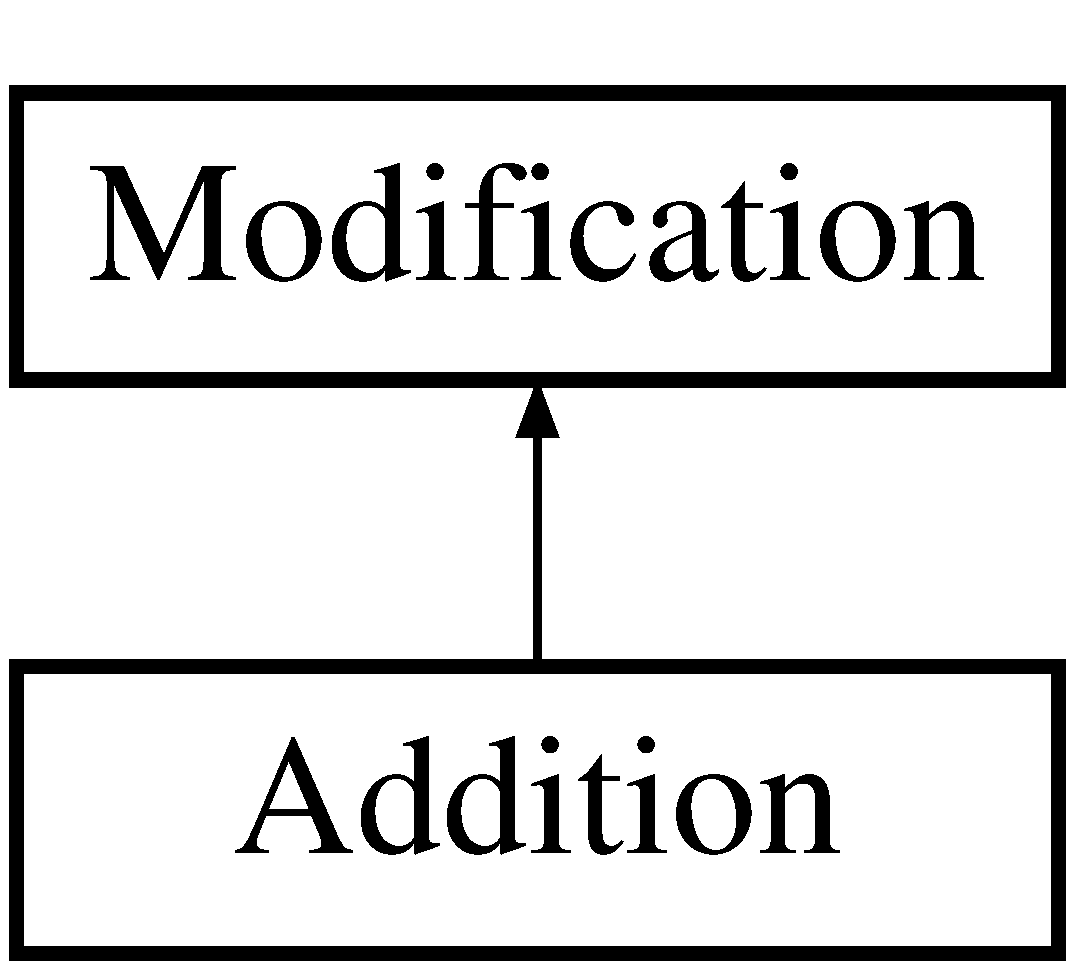
\includegraphics[height=2.000000cm]{class_addition}
\end{center}
\end{figure}
\subsection*{Public Member Functions}
\begin{DoxyCompactItemize}
\item 
\mbox{\hyperlink{class_addition_a0bcd6cd605c0e90a834339a1feb20901}{Addition}} (\mbox{\hyperlink{class_tree_object}{Tree\+Object}} $\ast$obj, \mbox{\hyperlink{class_tree_object}{Tree\+Object}} $\ast$parent)
\item 
\mbox{\hyperlink{class_addition_a66f0b31feefaaa51701e78b2a366b840}{$\sim$\+Addition}} ()
\item 
void \mbox{\hyperlink{class_addition_a08cd2dae96a62c80d6fe62339232fbca}{write\+\_\+out}} (\mbox{\hyperlink{class_partition_manager}{Partition\+Manager}} $\ast$pm)
\end{DoxyCompactItemize}
\subsection*{Additional Inherited Members}


\subsection{Constructor \& Destructor Documentation}
\mbox{\Hypertarget{class_addition_a0bcd6cd605c0e90a834339a1feb20901}\label{class_addition_a0bcd6cd605c0e90a834339a1feb20901}} 
\index{Addition@{Addition}!Addition@{Addition}}
\index{Addition@{Addition}!Addition@{Addition}}
\subsubsection{\texorpdfstring{Addition()}{Addition()}}
{\footnotesize\ttfamily Addition\+::\+Addition (\begin{DoxyParamCaption}\item[{\mbox{\hyperlink{class_tree_object}{Tree\+Object}} $\ast$}]{obj,  }\item[{\mbox{\hyperlink{class_tree_object}{Tree\+Object}} $\ast$}]{parent }\end{DoxyParamCaption})}

\mbox{\Hypertarget{class_addition_a66f0b31feefaaa51701e78b2a366b840}\label{class_addition_a66f0b31feefaaa51701e78b2a366b840}} 
\index{Addition@{Addition}!````~Addition@{$\sim$\+Addition}}
\index{````~Addition@{$\sim$\+Addition}!Addition@{Addition}}
\subsubsection{\texorpdfstring{$\sim$\+Addition()}{~Addition()}}
{\footnotesize\ttfamily Addition\+::$\sim$\+Addition (\begin{DoxyParamCaption}{ }\end{DoxyParamCaption})}



\subsection{Member Function Documentation}
\mbox{\Hypertarget{class_addition_a08cd2dae96a62c80d6fe62339232fbca}\label{class_addition_a08cd2dae96a62c80d6fe62339232fbca}} 
\index{Addition@{Addition}!write\+\_\+out@{write\+\_\+out}}
\index{write\+\_\+out@{write\+\_\+out}!Addition@{Addition}}
\subsubsection{\texorpdfstring{write\+\_\+out()}{write\_out()}}
{\footnotesize\ttfamily void Addition\+::write\+\_\+out (\begin{DoxyParamCaption}\item[{\mbox{\hyperlink{class_partition_manager}{Partition\+Manager}} $\ast$}]{pm }\end{DoxyParamCaption})\hspace{0.3cm}{\ttfamily [virtual]}}



Implements \mbox{\hyperlink{class_modification_a50d1fd809524902d2a1e78d02f4be1dc}{Modification}}.



The documentation for this class was generated from the following files\+:\begin{DoxyCompactItemize}
\item 
Filesystem/\+Daemon\+Dependancies/\+Trees/\mbox{\hyperlink{_trees_8h}{Trees.\+h}}\item 
Filesystem/\+Daemon\+Dependancies/\+Trees/\mbox{\hyperlink{_trees_8cpp}{Trees.\+cpp}}\end{DoxyCompactItemize}

\hypertarget{classarboreal__cli__error}{}\section{arboreal\+\_\+cli\+\_\+error Class Reference}
\label{classarboreal__cli__error}\index{arboreal\+\_\+cli\+\_\+error@{arboreal\+\_\+cli\+\_\+error}}
Inheritance diagram for arboreal\+\_\+cli\+\_\+error\+:\begin{figure}[H]
\begin{center}
\leavevmode
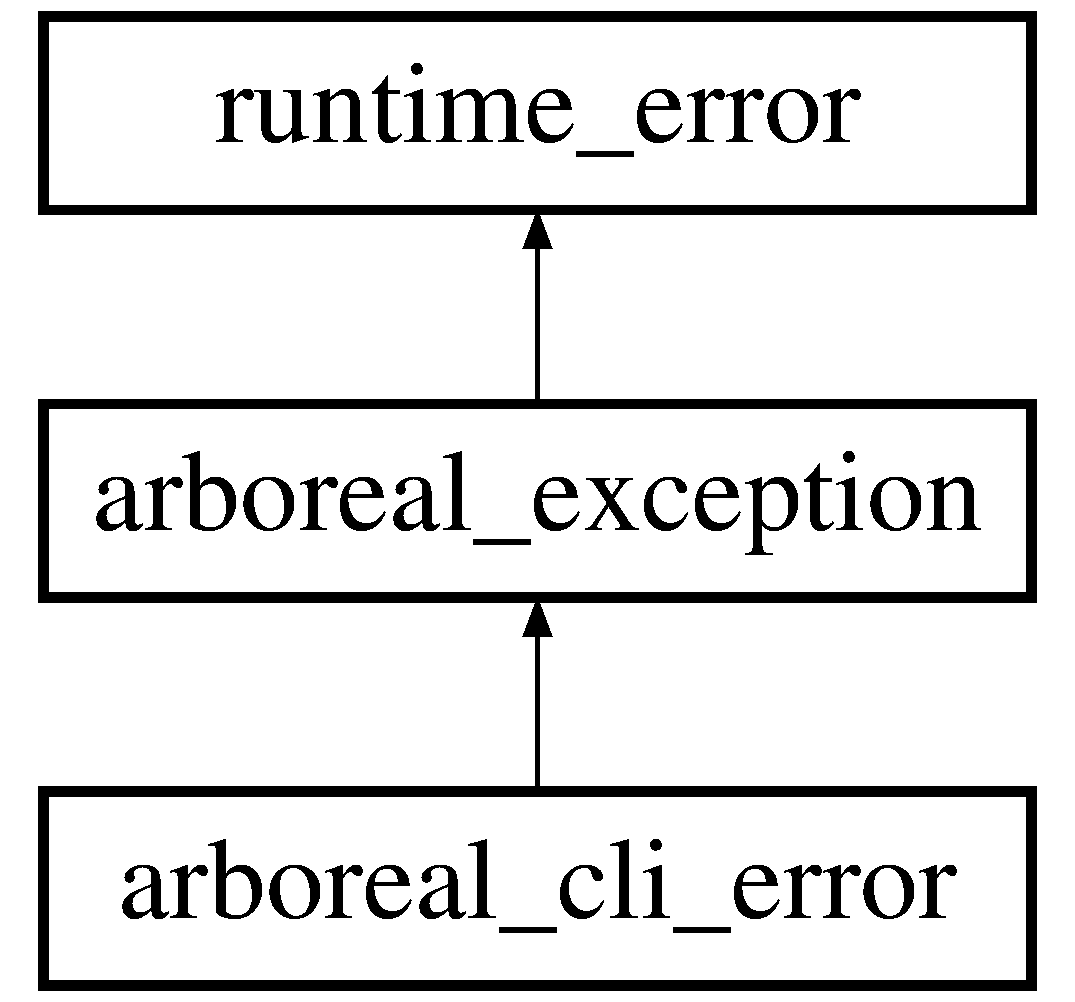
\includegraphics[height=3.000000cm]{d2/d7d/classarboreal__cli__error}
\end{center}
\end{figure}
\subsection*{Public Member Functions}
\begin{DoxyCompactItemize}
\item 
\mbox{\Hypertarget{classarboreal__cli__error_a39291e6c997b531c712892b9623f938a}\label{classarboreal__cli__error_a39291e6c997b531c712892b9623f938a}} 
{\bfseries arboreal\+\_\+cli\+\_\+error} (const string \&where, const string \&what, const int ecode=99)
\item 
\mbox{\Hypertarget{classarboreal__cli__error_adecf3ae0818fcdff4d375ef12ea1659e}\label{classarboreal__cli__error_adecf3ae0818fcdff4d375ef12ea1659e}} 
{\bfseries arboreal\+\_\+cli\+\_\+error} (const char $\ast$what, const char $\ast$where, const int ecode=99)
\item 
\mbox{\Hypertarget{classarboreal__cli__error_ab9388ea7e89c5232d7dd43d00019fef6}\label{classarboreal__cli__error_ab9388ea7e89c5232d7dd43d00019fef6}} 
{\bfseries arboreal\+\_\+cli\+\_\+error} (const char $\ast$what, const string \&where, const int ecode=99)
\item 
\mbox{\Hypertarget{classarboreal__cli__error_a297adfc95de15ebdceae7cf364d05600}\label{classarboreal__cli__error_a297adfc95de15ebdceae7cf364d05600}} 
{\bfseries arboreal\+\_\+cli\+\_\+error} (const string \&what, const char $\ast$where, const int ecode=99)
\end{DoxyCompactItemize}
\subsection*{Additional Inherited Members}


The documentation for this class was generated from the following files\+:\begin{DoxyCompactItemize}
\item 
Shared\+Headers/Arboreal\+\_\+\+Exceptions.\+h\item 
Shared\+C\+P\+P\+Files/Arboreal\+\_\+\+Exceptions.\+cpp\end{DoxyCompactItemize}

\hypertarget{classarboreal__daemon__error}{}\section{arboreal\+\_\+daemon\+\_\+error Class Reference}
\label{classarboreal__daemon__error}\index{arboreal\+\_\+daemon\+\_\+error@{arboreal\+\_\+daemon\+\_\+error}}
Inheritance diagram for arboreal\+\_\+daemon\+\_\+error\+:\begin{figure}[H]
\begin{center}
\leavevmode
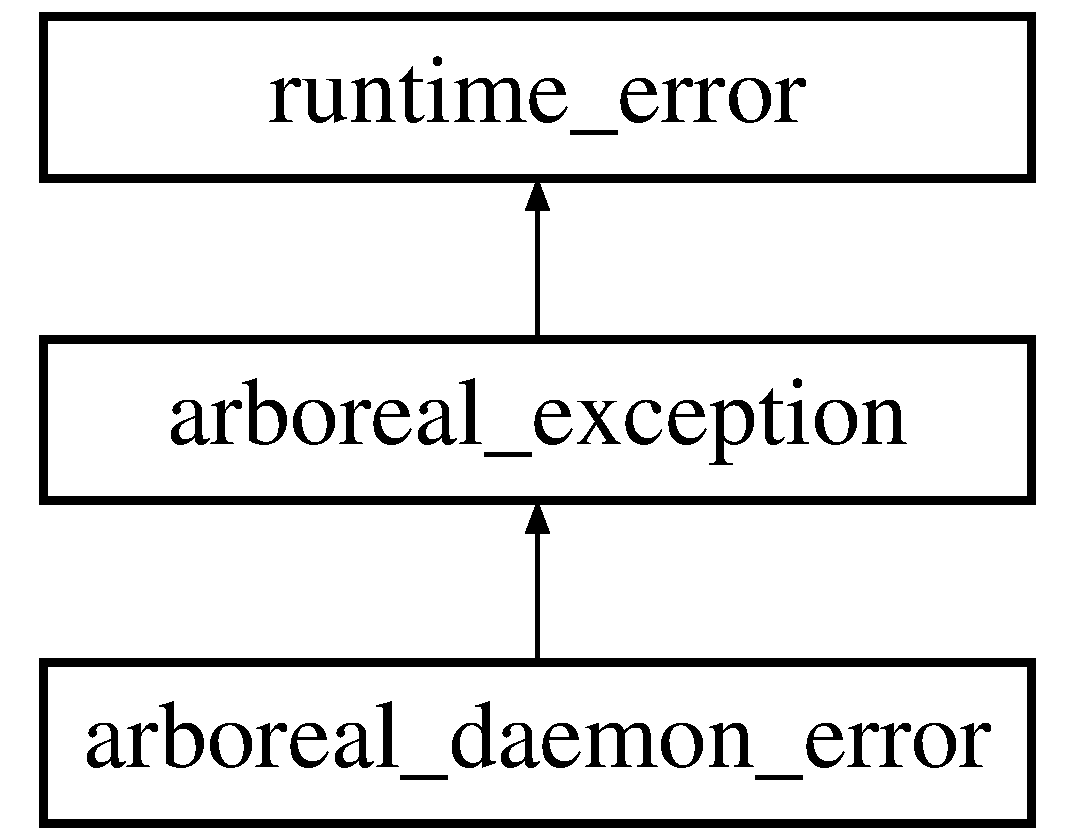
\includegraphics[height=3.000000cm]{db/d0e/classarboreal__daemon__error}
\end{center}
\end{figure}
\subsection*{Public Member Functions}
\begin{DoxyCompactItemize}
\item 
\mbox{\Hypertarget{classarboreal__daemon__error_aaa483ea710b1c20f37a61b7be7cd64fd}\label{classarboreal__daemon__error_aaa483ea710b1c20f37a61b7be7cd64fd}} 
{\bfseries arboreal\+\_\+daemon\+\_\+error} (const string \&where, const string \&what, const int ecode=99)
\item 
\mbox{\Hypertarget{classarboreal__daemon__error_a4a8b88442bf94bf88ffa162c8e8f76ef}\label{classarboreal__daemon__error_a4a8b88442bf94bf88ffa162c8e8f76ef}} 
{\bfseries arboreal\+\_\+daemon\+\_\+error} (const char $\ast$what, const char $\ast$where, const int ecode=99)
\item 
\mbox{\Hypertarget{classarboreal__daemon__error_a32d6c4b31f97c709952f44e15fd6bf8a}\label{classarboreal__daemon__error_a32d6c4b31f97c709952f44e15fd6bf8a}} 
{\bfseries arboreal\+\_\+daemon\+\_\+error} (const char $\ast$what, const string \&where, const int ecode=99)
\item 
\mbox{\Hypertarget{classarboreal__daemon__error_adc8e08526e65a9707c55b674c8d02044}\label{classarboreal__daemon__error_adc8e08526e65a9707c55b674c8d02044}} 
{\bfseries arboreal\+\_\+daemon\+\_\+error} (const string \&what, const char $\ast$where, const int ecode=99)
\end{DoxyCompactItemize}
\subsection*{Additional Inherited Members}


The documentation for this class was generated from the following files\+:\begin{DoxyCompactItemize}
\item 
Shared\+Headers/Arboreal\+\_\+\+Exceptions.\+h\item 
Shared\+C\+P\+P\+Files/Arboreal\+\_\+\+Exceptions.\+cpp\end{DoxyCompactItemize}

\hypertarget{classarboreal__exception}{}\section{arboreal\+\_\+exception Class Reference}
\label{classarboreal__exception}\index{arboreal\+\_\+exception@{arboreal\+\_\+exception}}
Inheritance diagram for arboreal\+\_\+exception\+:\begin{figure}[H]
\begin{center}
\leavevmode
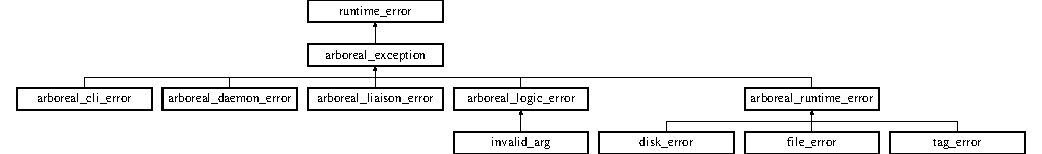
\includegraphics[height=3.684211cm]{classarboreal__exception}
\end{center}
\end{figure}
\subsection*{Public Member Functions}
\begin{DoxyCompactItemize}
\item 
\mbox{\Hypertarget{classarboreal__exception_a45ed8be47f52411504834440c481bc5f}\label{classarboreal__exception_a45ed8be47f52411504834440c481bc5f}} 
{\bfseries arboreal\+\_\+exception} (const char $\ast$what, const char $\ast$where)
\item 
\mbox{\Hypertarget{classarboreal__exception_a7d89267e972d47ac4052e3d6c94ee73b}\label{classarboreal__exception_a7d89267e972d47ac4052e3d6c94ee73b}} 
{\bfseries arboreal\+\_\+exception} (const char $\ast$what, const string \&where)
\item 
\mbox{\Hypertarget{classarboreal__exception_a3a3f2a7034c07dc5fe694ff860c0d4b4}\label{classarboreal__exception_a3a3f2a7034c07dc5fe694ff860c0d4b4}} 
{\bfseries arboreal\+\_\+exception} (const string \&what, const string \&where)
\item 
\mbox{\Hypertarget{classarboreal__exception_ac3099afc0a14eed3408dfffaac47d4ca}\label{classarboreal__exception_ac3099afc0a14eed3408dfffaac47d4ca}} 
{\bfseries arboreal\+\_\+exception} (const string \&what, const char $\ast$where)
\item 
\mbox{\Hypertarget{classarboreal__exception_a802003dee586aaeb0b0d7ce909da2dad}\label{classarboreal__exception_a802003dee586aaeb0b0d7ce909da2dad}} 
virtual const char $\ast$ {\bfseries where} () const
\end{DoxyCompactItemize}
\subsection*{Protected Attributes}
\begin{DoxyCompactItemize}
\item 
\mbox{\Hypertarget{classarboreal__exception_a73559e45af28b0804b66b04df4c04270}\label{classarboreal__exception_a73559e45af28b0804b66b04df4c04270}} 
string {\bfseries \+\_\+where}
\end{DoxyCompactItemize}


The documentation for this class was generated from the following files\+:\begin{DoxyCompactItemize}
\item 
Arboreal\+\_\+\+Exceptions.\+h\item 
Arboreal\+\_\+\+Exceptions.\+cpp\end{DoxyCompactItemize}

\hypertarget{classarboreal__liaison__error}{}\section{arboreal\+\_\+liaison\+\_\+error Class Reference}
\label{classarboreal__liaison__error}\index{arboreal\+\_\+liaison\+\_\+error@{arboreal\+\_\+liaison\+\_\+error}}
Inheritance diagram for arboreal\+\_\+liaison\+\_\+error\+:\begin{figure}[H]
\begin{center}
\leavevmode
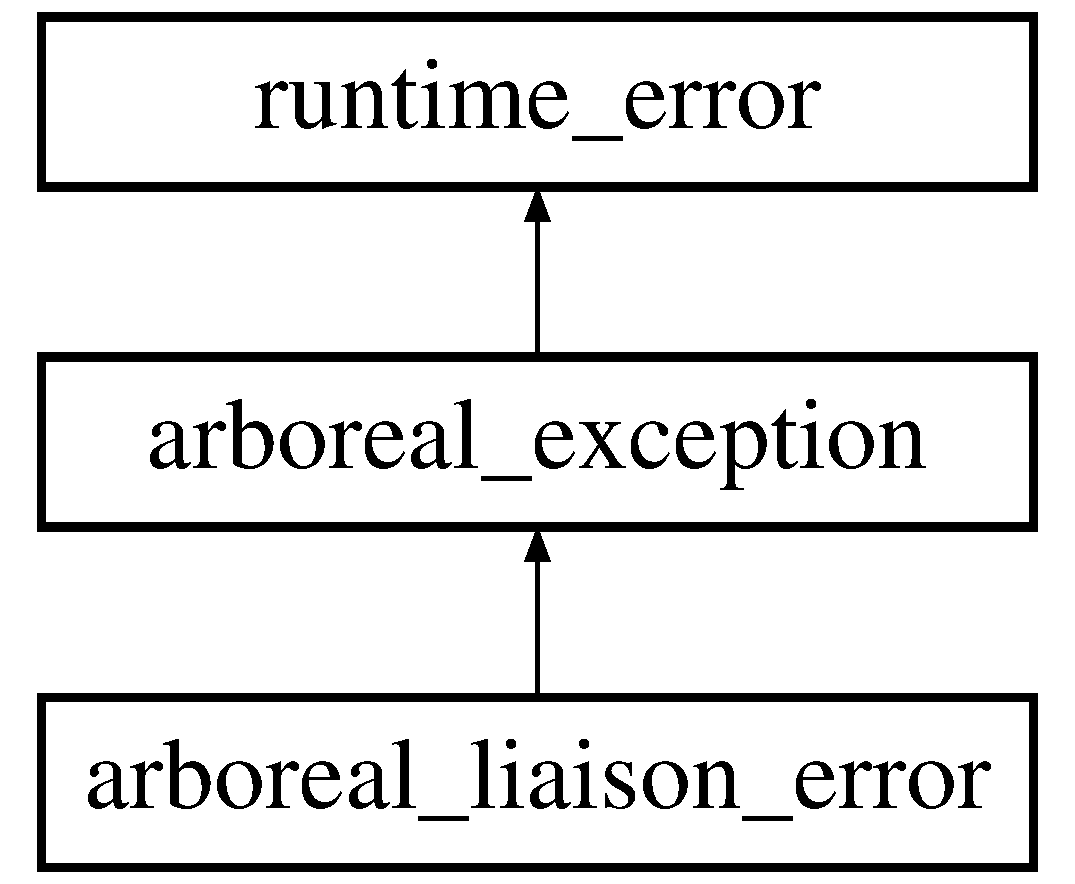
\includegraphics[height=3.000000cm]{classarboreal__liaison__error}
\end{center}
\end{figure}
\subsection*{Public Member Functions}
\begin{DoxyCompactItemize}
\item 
{\bfseries arboreal\+\_\+liaison\+\_\+error} (const string \&where, const string \&what, const int ecode=99)\hypertarget{classarboreal__liaison__error_af23c4a3672c9594e3382a05a1590abc4}{}\label{classarboreal__liaison__error_af23c4a3672c9594e3382a05a1590abc4}

\item 
{\bfseries arboreal\+\_\+liaison\+\_\+error} (const char $\ast$what, const char $\ast$where, const int ecode=99)\hypertarget{classarboreal__liaison__error_ae9eaf00df34e37262348e254c6dad5ff}{}\label{classarboreal__liaison__error_ae9eaf00df34e37262348e254c6dad5ff}

\item 
{\bfseries arboreal\+\_\+liaison\+\_\+error} (const char $\ast$what, const string \&where, const int ecode=99)\hypertarget{classarboreal__liaison__error_a593436824d649179f5c34b7311c56d2e}{}\label{classarboreal__liaison__error_a593436824d649179f5c34b7311c56d2e}

\item 
{\bfseries arboreal\+\_\+liaison\+\_\+error} (const string \&what, const char $\ast$where, const int ecode=99)\hypertarget{classarboreal__liaison__error_a73221c813d25af214f19eaec704ffffd}{}\label{classarboreal__liaison__error_a73221c813d25af214f19eaec704ffffd}

\end{DoxyCompactItemize}
\subsection*{Additional Inherited Members}


The documentation for this class was generated from the following files\+:\begin{DoxyCompactItemize}
\item 
Shared\+Headers/Arboreal\+\_\+\+Exceptions.\+h\item 
Shared\+C\+P\+P\+Files/Arboreal\+\_\+\+Exceptions.\+cpp\end{DoxyCompactItemize}

\hypertarget{classarboreal__logic__error}{}\section{arboreal\+\_\+logic\+\_\+error Class Reference}
\label{classarboreal__logic__error}\index{arboreal\+\_\+logic\+\_\+error@{arboreal\+\_\+logic\+\_\+error}}
Inheritance diagram for arboreal\+\_\+logic\+\_\+error\+:\begin{figure}[H]
\begin{center}
\leavevmode
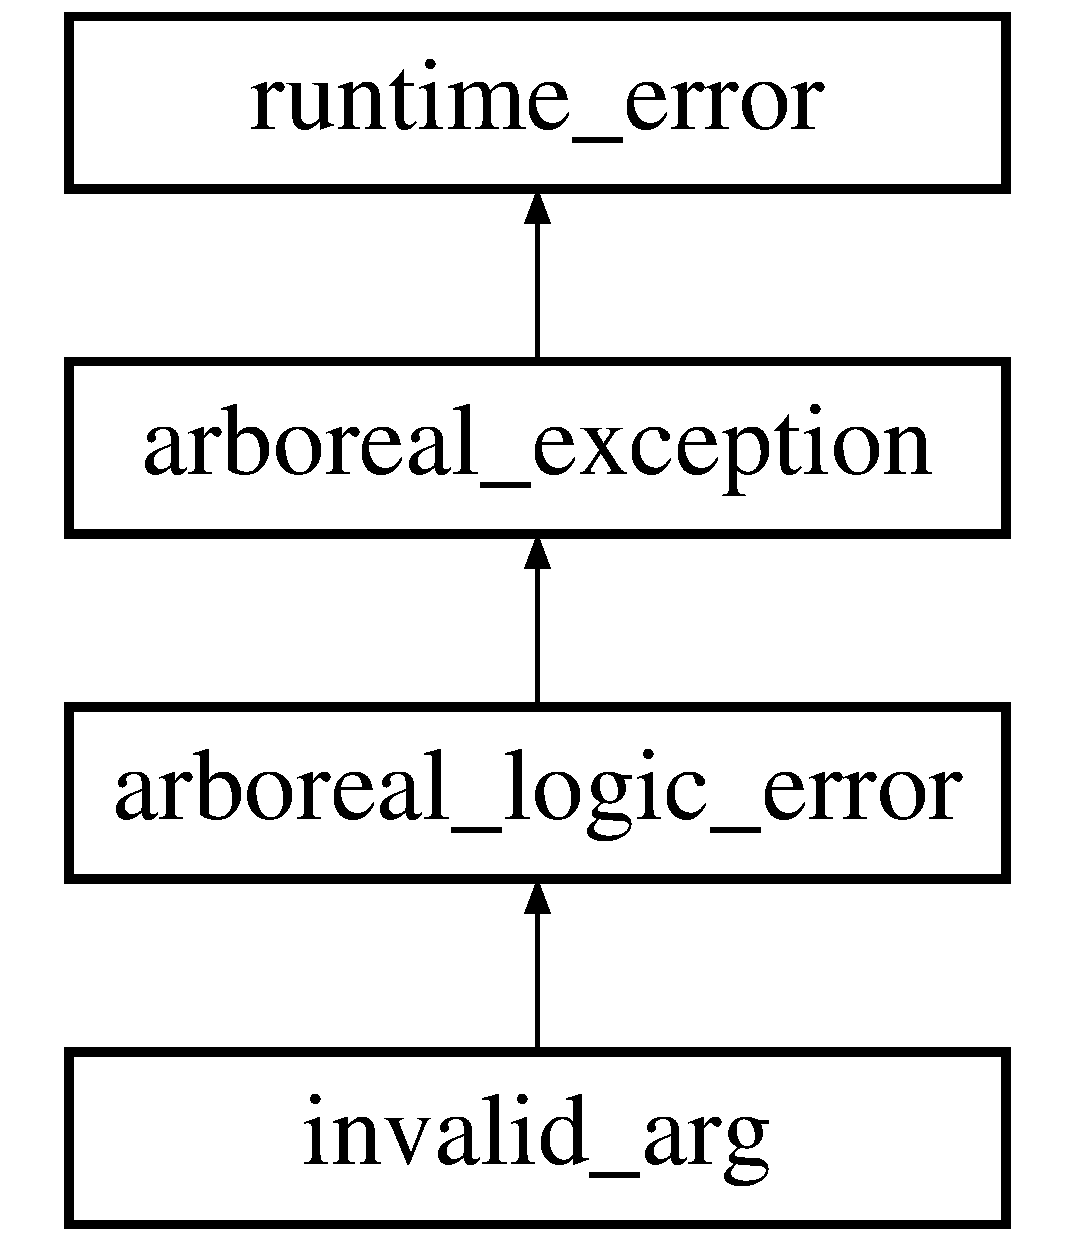
\includegraphics[height=4.000000cm]{classarboreal__logic__error}
\end{center}
\end{figure}
\subsection*{Public Member Functions}
\begin{DoxyCompactItemize}
\item 
{\bfseries arboreal\+\_\+logic\+\_\+error} (const char $\ast$what, const char $\ast$where, const int ecode=99)\hypertarget{classarboreal__logic__error_aaea786c69fe107f9b6753b51001c59d6}{}\label{classarboreal__logic__error_aaea786c69fe107f9b6753b51001c59d6}

\item 
{\bfseries arboreal\+\_\+logic\+\_\+error} (const char $\ast$what, const string \&where, const int ecode=99)\hypertarget{classarboreal__logic__error_a70b8217c9841efc9bb1e556282a89fe0}{}\label{classarboreal__logic__error_a70b8217c9841efc9bb1e556282a89fe0}

\item 
{\bfseries arboreal\+\_\+logic\+\_\+error} (const string \&what, const string \&where, const int ecode=99)\hypertarget{classarboreal__logic__error_ad7627c19a966b137cf018aa7c3075421}{}\label{classarboreal__logic__error_ad7627c19a966b137cf018aa7c3075421}

\item 
{\bfseries arboreal\+\_\+logic\+\_\+error} (const string \&what, const char $\ast$where, const int ecode=99)\hypertarget{classarboreal__logic__error_a5c589df18299902a24dae25f8a25c02a}{}\label{classarboreal__logic__error_a5c589df18299902a24dae25f8a25c02a}

\end{DoxyCompactItemize}
\subsection*{Additional Inherited Members}


The documentation for this class was generated from the following files\+:\begin{DoxyCompactItemize}
\item 
Shared\+Headers/Arboreal\+\_\+\+Exceptions.\+h\item 
Shared\+C\+P\+P\+Files/Arboreal\+\_\+\+Exceptions.\+cpp\end{DoxyCompactItemize}

\hypertarget{classarboreal__runtime__error}{}\section{arboreal\+\_\+runtime\+\_\+error Class Reference}
\label{classarboreal__runtime__error}\index{arboreal\+\_\+runtime\+\_\+error@{arboreal\+\_\+runtime\+\_\+error}}
Inheritance diagram for arboreal\+\_\+runtime\+\_\+error\+:\begin{figure}[H]
\begin{center}
\leavevmode
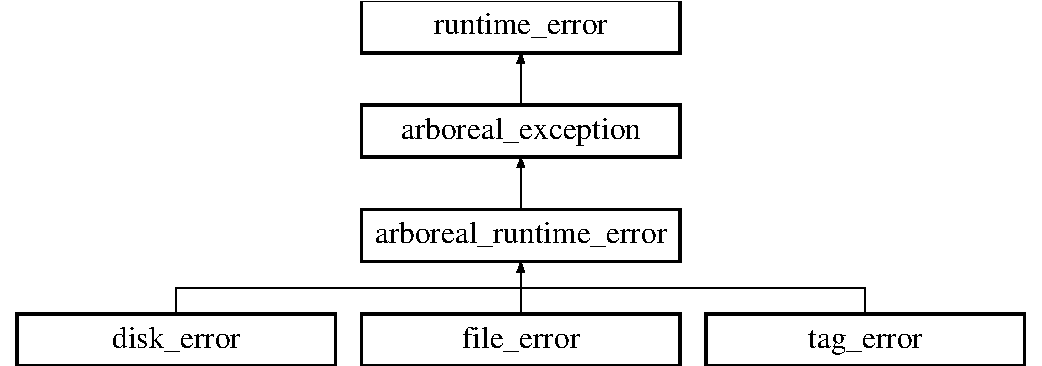
\includegraphics[height=4.000000cm]{classarboreal__runtime__error}
\end{center}
\end{figure}
\subsection*{Public Member Functions}
\begin{DoxyCompactItemize}
\item 
{\bfseries arboreal\+\_\+runtime\+\_\+error} (const char $\ast$what, const char $\ast$where, const int ecode=99)\hypertarget{classarboreal__runtime__error_aa6970966b569a105ead4fc6a5648cb5e}{}\label{classarboreal__runtime__error_aa6970966b569a105ead4fc6a5648cb5e}

\item 
{\bfseries arboreal\+\_\+runtime\+\_\+error} (const char $\ast$what, const string \&where, const int ecode=99)\hypertarget{classarboreal__runtime__error_af20cdd8f990b40293bbbf11f3fe1005b}{}\label{classarboreal__runtime__error_af20cdd8f990b40293bbbf11f3fe1005b}

\item 
{\bfseries arboreal\+\_\+runtime\+\_\+error} (const string \&what, const string \&where, const int ecode=99)\hypertarget{classarboreal__runtime__error_a3797d6f9ba8c5590539b280042d023a5}{}\label{classarboreal__runtime__error_a3797d6f9ba8c5590539b280042d023a5}

\item 
{\bfseries arboreal\+\_\+runtime\+\_\+error} (const string \&what, const char $\ast$where, const int ecode=99)\hypertarget{classarboreal__runtime__error_a897b94adcbe8bdbcd8c7299d95c4e020}{}\label{classarboreal__runtime__error_a897b94adcbe8bdbcd8c7299d95c4e020}

\end{DoxyCompactItemize}
\subsection*{Protected Attributes}
\begin{DoxyCompactItemize}
\item 
string {\bfseries \+\_\+where}\hypertarget{classarboreal__runtime__error_afca0adf6a259600843b6975591e0bde4}{}\label{classarboreal__runtime__error_afca0adf6a259600843b6975591e0bde4}

\item 
int {\bfseries \+\_\+ecode}\hypertarget{classarboreal__runtime__error_a08953e7ed35ac7db0d86032a3eb3f837}{}\label{classarboreal__runtime__error_a08953e7ed35ac7db0d86032a3eb3f837}

\end{DoxyCompactItemize}


The documentation for this class was generated from the following files\+:\begin{DoxyCompactItemize}
\item 
Shared\+Headers/Arboreal\+\_\+\+Exceptions.\+h\item 
Shared\+C\+P\+P\+Files/Arboreal\+\_\+\+Exceptions.\+cpp\end{DoxyCompactItemize}

\hypertarget{class_attributes}{}\section{Attributes Class Reference}
\label{class_attributes}\index{Attributes@{Attributes}}


{\ttfamily \#include $<$Trees.\+h$>$}

\subsection*{Public Member Functions}
\begin{DoxyCompactItemize}
\item 
\mbox{\hyperlink{class_attributes_a0d6b154029e34f811f0930806768f022}{Attributes}} (Blk\+Num\+Type blknum, \mbox{\hyperlink{class_partition_manager}{Partition\+Manager}} $\ast$pm)
\end{DoxyCompactItemize}
\begin{Indent}\textbf{ Modifier Functions}\par
\begin{DoxyCompactItemize}
\item 
void \mbox{\hyperlink{class_attributes_a7066f30d97317f75a02a137d09a2065e}{write\+\_\+out}} ()
\item 
void \mbox{\hyperlink{class_attributes_ac33fbd6871ef707878690be92b9fc7ec}{read\+\_\+in}} ()
\item 
void \mbox{\hyperlink{class_attributes_acf28e724c914f066ecdae788d95b3212}{del}} ()
\item 
void \mbox{\hyperlink{class_attributes_a4c518dae976d9186337f655f7b09cecc}{set\+\_\+creation\+\_\+time}} ()
\item 
void \mbox{\hyperlink{class_attributes_affdf3abb52a45ac3c9051bafd0da9e7e}{set\+\_\+owner}} (int owner)
\item 
void \mbox{\hyperlink{class_attributes_aac8ca00f98b22280df69f62e42b72b8b}{set\+\_\+permissions}} (char $\ast$perms)
\item 
void \mbox{\hyperlink{class_attributes_af2ce6f6dce652a7adfeba3f28b4ee0bc}{set\+\_\+access}} ()
\item 
void \mbox{\hyperlink{class_attributes_a88674bf65fba99d32870c7fa48edf135}{set\+\_\+edit}} ()
\item 
void \mbox{\hyperlink{class_attributes_a3983ec45af66e9b19367222092b7df6c}{update\+\_\+size}} (size\+\_\+t size)
\end{DoxyCompactItemize}
\end{Indent}
\begin{Indent}\textbf{ Accessor Functions}\par
\begin{DoxyCompactItemize}
\item 
time\+\_\+t \mbox{\hyperlink{class_attributes_aeb0845464130e292875be4f8dcc51e8a}{get\+\_\+creation\+\_\+time}} ()
\item 
int \mbox{\hyperlink{class_attributes_a8b9efe0186ccf74b4b08c4031a99f5bb}{get\+\_\+owner}} ()
\item 
char $\ast$ \mbox{\hyperlink{class_attributes_a52a8dc1b5d9c4c1eb19bcb336705cc42}{get\+\_\+permissions}} ()
\item 
time\+\_\+t \mbox{\hyperlink{class_attributes_a9cd0c49733d3de43a8916a318ba62bc1}{get\+\_\+access}} ()
\item 
time\+\_\+t \mbox{\hyperlink{class_attributes_a4ff80c2f3a31f86d874d7982354e4f70}{get\+\_\+edit}} ()
\item 
size\+\_\+t \mbox{\hyperlink{class_attributes_a6e5df8252fc902c0fbe22058fe0b4fb1}{get\+\_\+size}} ()
\item 
File\+Attributes \mbox{\hyperlink{class_attributes_a774666651c1d61cade39cc15cf03b9b2}{get\+\_\+file\+\_\+attributes}} ()
\end{DoxyCompactItemize}
\end{Indent}
\subsection*{Private Attributes}
\begin{DoxyCompactItemize}
\item 
File\+Attributes \mbox{\hyperlink{class_attributes_adb049fd16001d1634a6534917dcaf8c3}{\+\_\+atts}}
\item 
Blk\+Num\+Type \mbox{\hyperlink{class_attributes_a58984b59c6cf95453f54824113a95d67}{\+\_\+block\+Number}}
\item 
\mbox{\hyperlink{class_partition_manager}{Partition\+Manager}} $\ast$ \mbox{\hyperlink{class_attributes_ae344a55e94b87cbc3cb9e956f5753eee}{\+\_\+my\+Partition\+Manager}}
\end{DoxyCompactItemize}


\subsection{Constructor \& Destructor Documentation}
\mbox{\Hypertarget{class_attributes_a0d6b154029e34f811f0930806768f022}\label{class_attributes_a0d6b154029e34f811f0930806768f022}} 
\index{Attributes@{Attributes}!Attributes@{Attributes}}
\index{Attributes@{Attributes}!Attributes@{Attributes}}
\subsubsection{\texorpdfstring{Attributes()}{Attributes()}}
{\footnotesize\ttfamily Attributes\+::\+Attributes (\begin{DoxyParamCaption}\item[{Blk\+Num\+Type}]{blknum,  }\item[{\mbox{\hyperlink{class_partition_manager}{Partition\+Manager}} $\ast$}]{pm }\end{DoxyParamCaption})}



\subsection{Member Function Documentation}
\mbox{\Hypertarget{class_attributes_acf28e724c914f066ecdae788d95b3212}\label{class_attributes_acf28e724c914f066ecdae788d95b3212}} 
\index{Attributes@{Attributes}!del@{del}}
\index{del@{del}!Attributes@{Attributes}}
\subsubsection{\texorpdfstring{del()}{del()}}
{\footnotesize\ttfamily void Attributes\+::del (\begin{DoxyParamCaption}{ }\end{DoxyParamCaption})}

Removes the \mbox{\hyperlink{class_attributes}{Attributes}} presence on disk \mbox{\Hypertarget{class_attributes_a9cd0c49733d3de43a8916a318ba62bc1}\label{class_attributes_a9cd0c49733d3de43a8916a318ba62bc1}} 
\index{Attributes@{Attributes}!get\+\_\+access@{get\+\_\+access}}
\index{get\+\_\+access@{get\+\_\+access}!Attributes@{Attributes}}
\subsubsection{\texorpdfstring{get\+\_\+access()}{get\_access()}}
{\footnotesize\ttfamily time\+\_\+t Attributes\+::get\+\_\+access (\begin{DoxyParamCaption}{ }\end{DoxyParamCaption})}

\begin{DoxyReturn}{Returns}
the U\+N\+IX time the file was last accessed 
\end{DoxyReturn}
\mbox{\Hypertarget{class_attributes_aeb0845464130e292875be4f8dcc51e8a}\label{class_attributes_aeb0845464130e292875be4f8dcc51e8a}} 
\index{Attributes@{Attributes}!get\+\_\+creation\+\_\+time@{get\+\_\+creation\+\_\+time}}
\index{get\+\_\+creation\+\_\+time@{get\+\_\+creation\+\_\+time}!Attributes@{Attributes}}
\subsubsection{\texorpdfstring{get\+\_\+creation\+\_\+time()}{get\_creation\_time()}}
{\footnotesize\ttfamily time\+\_\+t Attributes\+::get\+\_\+creation\+\_\+time (\begin{DoxyParamCaption}{ }\end{DoxyParamCaption})}

\begin{DoxyReturn}{Returns}
the U\+N\+IX time the file was created 
\end{DoxyReturn}
\mbox{\Hypertarget{class_attributes_a4ff80c2f3a31f86d874d7982354e4f70}\label{class_attributes_a4ff80c2f3a31f86d874d7982354e4f70}} 
\index{Attributes@{Attributes}!get\+\_\+edit@{get\+\_\+edit}}
\index{get\+\_\+edit@{get\+\_\+edit}!Attributes@{Attributes}}
\subsubsection{\texorpdfstring{get\+\_\+edit()}{get\_edit()}}
{\footnotesize\ttfamily time\+\_\+t Attributes\+::get\+\_\+edit (\begin{DoxyParamCaption}{ }\end{DoxyParamCaption})}

\begin{DoxyReturn}{Returns}
the U\+N\+IX time the file was last edited 
\end{DoxyReturn}
\mbox{\Hypertarget{class_attributes_a774666651c1d61cade39cc15cf03b9b2}\label{class_attributes_a774666651c1d61cade39cc15cf03b9b2}} 
\index{Attributes@{Attributes}!get\+\_\+file\+\_\+attributes@{get\+\_\+file\+\_\+attributes}}
\index{get\+\_\+file\+\_\+attributes@{get\+\_\+file\+\_\+attributes}!Attributes@{Attributes}}
\subsubsection{\texorpdfstring{get\+\_\+file\+\_\+attributes()}{get\_file\_attributes()}}
{\footnotesize\ttfamily File\+Attributes Attributes\+::get\+\_\+file\+\_\+attributes (\begin{DoxyParamCaption}{ }\end{DoxyParamCaption})}

\begin{DoxyReturn}{Returns}
the entire File\+Attributes struct 
\end{DoxyReturn}
\mbox{\Hypertarget{class_attributes_a8b9efe0186ccf74b4b08c4031a99f5bb}\label{class_attributes_a8b9efe0186ccf74b4b08c4031a99f5bb}} 
\index{Attributes@{Attributes}!get\+\_\+owner@{get\+\_\+owner}}
\index{get\+\_\+owner@{get\+\_\+owner}!Attributes@{Attributes}}
\subsubsection{\texorpdfstring{get\+\_\+owner()}{get\_owner()}}
{\footnotesize\ttfamily int Attributes\+::get\+\_\+owner (\begin{DoxyParamCaption}{ }\end{DoxyParamCaption})}

\begin{DoxyReturn}{Returns}
the U\+ID of the owner of the file 
\end{DoxyReturn}
\mbox{\Hypertarget{class_attributes_a52a8dc1b5d9c4c1eb19bcb336705cc42}\label{class_attributes_a52a8dc1b5d9c4c1eb19bcb336705cc42}} 
\index{Attributes@{Attributes}!get\+\_\+permissions@{get\+\_\+permissions}}
\index{get\+\_\+permissions@{get\+\_\+permissions}!Attributes@{Attributes}}
\subsubsection{\texorpdfstring{get\+\_\+permissions()}{get\_permissions()}}
{\footnotesize\ttfamily char $\ast$ Attributes\+::get\+\_\+permissions (\begin{DoxyParamCaption}{ }\end{DoxyParamCaption})}

\begin{DoxyReturn}{Returns}
the permisssions 
\end{DoxyReturn}
\begin{DoxySeeAlso}{See also}
File\+Info\+::get\+\_\+permissions(char$\ast$) 
\end{DoxySeeAlso}
\mbox{\Hypertarget{class_attributes_a6e5df8252fc902c0fbe22058fe0b4fb1}\label{class_attributes_a6e5df8252fc902c0fbe22058fe0b4fb1}} 
\index{Attributes@{Attributes}!get\+\_\+size@{get\+\_\+size}}
\index{get\+\_\+size@{get\+\_\+size}!Attributes@{Attributes}}
\subsubsection{\texorpdfstring{get\+\_\+size()}{get\_size()}}
{\footnotesize\ttfamily size\+\_\+t Attributes\+::get\+\_\+size (\begin{DoxyParamCaption}{ }\end{DoxyParamCaption})}

\begin{DoxyReturn}{Returns}
the size of the file in bytes 
\end{DoxyReturn}
\mbox{\Hypertarget{class_attributes_ac33fbd6871ef707878690be92b9fc7ec}\label{class_attributes_ac33fbd6871ef707878690be92b9fc7ec}} 
\index{Attributes@{Attributes}!read\+\_\+in@{read\+\_\+in}}
\index{read\+\_\+in@{read\+\_\+in}!Attributes@{Attributes}}
\subsubsection{\texorpdfstring{read\+\_\+in()}{read\_in()}}
{\footnotesize\ttfamily void Attributes\+::read\+\_\+in (\begin{DoxyParamCaption}{ }\end{DoxyParamCaption})}

Reads in the \mbox{\hyperlink{class_attributes}{Attributes}} from disk \mbox{\Hypertarget{class_attributes_af2ce6f6dce652a7adfeba3f28b4ee0bc}\label{class_attributes_af2ce6f6dce652a7adfeba3f28b4ee0bc}} 
\index{Attributes@{Attributes}!set\+\_\+access@{set\+\_\+access}}
\index{set\+\_\+access@{set\+\_\+access}!Attributes@{Attributes}}
\subsubsection{\texorpdfstring{set\+\_\+access()}{set\_access()}}
{\footnotesize\ttfamily void Attributes\+::set\+\_\+access (\begin{DoxyParamCaption}{ }\end{DoxyParamCaption})}

Marks down the time as accessed time as U\+N\+IX timestamp \mbox{\Hypertarget{class_attributes_a4c518dae976d9186337f655f7b09cecc}\label{class_attributes_a4c518dae976d9186337f655f7b09cecc}} 
\index{Attributes@{Attributes}!set\+\_\+creation\+\_\+time@{set\+\_\+creation\+\_\+time}}
\index{set\+\_\+creation\+\_\+time@{set\+\_\+creation\+\_\+time}!Attributes@{Attributes}}
\subsubsection{\texorpdfstring{set\+\_\+creation\+\_\+time()}{set\_creation\_time()}}
{\footnotesize\ttfamily void Attributes\+::set\+\_\+creation\+\_\+time (\begin{DoxyParamCaption}{ }\end{DoxyParamCaption})}

Marks down the creation time of the associated \mbox{\hyperlink{class_file_info}{File\+Info}} as U\+N\+IX timestamp \mbox{\Hypertarget{class_attributes_a88674bf65fba99d32870c7fa48edf135}\label{class_attributes_a88674bf65fba99d32870c7fa48edf135}} 
\index{Attributes@{Attributes}!set\+\_\+edit@{set\+\_\+edit}}
\index{set\+\_\+edit@{set\+\_\+edit}!Attributes@{Attributes}}
\subsubsection{\texorpdfstring{set\+\_\+edit()}{set\_edit()}}
{\footnotesize\ttfamily void Attributes\+::set\+\_\+edit (\begin{DoxyParamCaption}{ }\end{DoxyParamCaption})}

Marks down the time as modified time as U\+N\+IX timestamp \mbox{\Hypertarget{class_attributes_affdf3abb52a45ac3c9051bafd0da9e7e}\label{class_attributes_affdf3abb52a45ac3c9051bafd0da9e7e}} 
\index{Attributes@{Attributes}!set\+\_\+owner@{set\+\_\+owner}}
\index{set\+\_\+owner@{set\+\_\+owner}!Attributes@{Attributes}}
\subsubsection{\texorpdfstring{set\+\_\+owner()}{set\_owner()}}
{\footnotesize\ttfamily void Attributes\+::set\+\_\+owner (\begin{DoxyParamCaption}\item[{int}]{owner }\end{DoxyParamCaption})}

Marks the owner as their U\+ID \mbox{\Hypertarget{class_attributes_aac8ca00f98b22280df69f62e42b72b8b}\label{class_attributes_aac8ca00f98b22280df69f62e42b72b8b}} 
\index{Attributes@{Attributes}!set\+\_\+permissions@{set\+\_\+permissions}}
\index{set\+\_\+permissions@{set\+\_\+permissions}!Attributes@{Attributes}}
\subsubsection{\texorpdfstring{set\+\_\+permissions()}{set\_permissions()}}
{\footnotesize\ttfamily void Attributes\+::set\+\_\+permissions (\begin{DoxyParamCaption}\item[{char $\ast$}]{perms }\end{DoxyParamCaption})}

sets the permisssions of the file \begin{DoxySeeAlso}{See also}
\mbox{\hyperlink{class_file_info_a377208012195dba0b24723837f6db39f}{File\+Info\+::set\+\_\+permissions(char$\ast$)}} 
\end{DoxySeeAlso}
\mbox{\Hypertarget{class_attributes_a3983ec45af66e9b19367222092b7df6c}\label{class_attributes_a3983ec45af66e9b19367222092b7df6c}} 
\index{Attributes@{Attributes}!update\+\_\+size@{update\+\_\+size}}
\index{update\+\_\+size@{update\+\_\+size}!Attributes@{Attributes}}
\subsubsection{\texorpdfstring{update\+\_\+size()}{update\_size()}}
{\footnotesize\ttfamily void Attributes\+::update\+\_\+size (\begin{DoxyParamCaption}\item[{size\+\_\+t}]{size }\end{DoxyParamCaption})}

sets the size to the specified size \mbox{\Hypertarget{class_attributes_a7066f30d97317f75a02a137d09a2065e}\label{class_attributes_a7066f30d97317f75a02a137d09a2065e}} 
\index{Attributes@{Attributes}!write\+\_\+out@{write\+\_\+out}}
\index{write\+\_\+out@{write\+\_\+out}!Attributes@{Attributes}}
\subsubsection{\texorpdfstring{write\+\_\+out()}{write\_out()}}
{\footnotesize\ttfamily void Attributes\+::write\+\_\+out (\begin{DoxyParamCaption}{ }\end{DoxyParamCaption})}

Writes out the \mbox{\hyperlink{class_attributes}{Attributes}} to disk 

\subsection{Member Data Documentation}
\mbox{\Hypertarget{class_attributes_adb049fd16001d1634a6534917dcaf8c3}\label{class_attributes_adb049fd16001d1634a6534917dcaf8c3}} 
\index{Attributes@{Attributes}!\+\_\+atts@{\+\_\+atts}}
\index{\+\_\+atts@{\+\_\+atts}!Attributes@{Attributes}}
\subsubsection{\texorpdfstring{\+\_\+atts}{\_atts}}
{\footnotesize\ttfamily File\+Attributes Attributes\+::\+\_\+atts\hspace{0.3cm}{\ttfamily [private]}}

\mbox{\Hypertarget{class_attributes_a58984b59c6cf95453f54824113a95d67}\label{class_attributes_a58984b59c6cf95453f54824113a95d67}} 
\index{Attributes@{Attributes}!\+\_\+block\+Number@{\+\_\+block\+Number}}
\index{\+\_\+block\+Number@{\+\_\+block\+Number}!Attributes@{Attributes}}
\subsubsection{\texorpdfstring{\+\_\+block\+Number}{\_blockNumber}}
{\footnotesize\ttfamily Blk\+Num\+Type Attributes\+::\+\_\+block\+Number\hspace{0.3cm}{\ttfamily [private]}}

\mbox{\Hypertarget{class_attributes_ae344a55e94b87cbc3cb9e956f5753eee}\label{class_attributes_ae344a55e94b87cbc3cb9e956f5753eee}} 
\index{Attributes@{Attributes}!\+\_\+my\+Partition\+Manager@{\+\_\+my\+Partition\+Manager}}
\index{\+\_\+my\+Partition\+Manager@{\+\_\+my\+Partition\+Manager}!Attributes@{Attributes}}
\subsubsection{\texorpdfstring{\+\_\+my\+Partition\+Manager}{\_myPartitionManager}}
{\footnotesize\ttfamily \mbox{\hyperlink{class_partition_manager}{Partition\+Manager}}$\ast$ Attributes\+::\+\_\+my\+Partition\+Manager\hspace{0.3cm}{\ttfamily [private]}}



The documentation for this class was generated from the following files\+:\begin{DoxyCompactItemize}
\item 
Filesystem/\+Daemon\+Dependancies/\+Trees/\mbox{\hyperlink{_trees_8h}{Trees.\+h}}\item 
Filesystem/\+Daemon\+Dependancies/\+Trees/\mbox{\hyperlink{_trees_8cpp}{Trees.\+cpp}}\end{DoxyCompactItemize}

\hypertarget{class_debug_messages}{}\section{Debug\+Messages Class Reference}
\label{class_debug_messages}\index{Debug\+Messages@{Debug\+Messages}}


{\ttfamily \#include $<$Debug\+Messages.\+h$>$}

\subsection*{Public Member Functions}
\begin{DoxyCompactItemize}
\item 
\mbox{\hyperlink{class_debug_messages_a7fb2c5a7cce97eb05661b1f6657cb650}{Debug\+Messages}} ()
\item 
\mbox{\hyperlink{class_debug_messages_aa60430ca0e05e43a8bb27f4cdc1a158c}{Debug\+Messages}} (std\+::string logfile\+\_\+name)
\item 
\mbox{\hyperlink{class_debug_messages_a3700e476ad70d27ba14be67b43ff6f69}{$\sim$\+Debug\+Messages}} ()
\item 
void \mbox{\hyperlink{class_debug_messages_a9a73bcf5d8298fd68b55a28c0878e852}{display}} (const \mbox{\hyperlink{_debug_messages_8h_a0da83e35f29c11f7f3c637234f2149f9}{Control}} flow)
\item 
void \mbox{\hyperlink{class_debug_messages_a802f7d26dedc412f06bfe0957415bfd4}{log}} (const \mbox{\hyperlink{_debug_messages_8h_a0da83e35f29c11f7f3c637234f2149f9}{Control}} flow)
\item 
void \mbox{\hyperlink{class_debug_messages_a5cd8aa8eb917f7da19484adc2c7e31a2}{debug}} (const \mbox{\hyperlink{_debug_messages_8h_a0da83e35f29c11f7f3c637234f2149f9}{Control}} flow)
\item 
void \mbox{\hyperlink{class_debug_messages_a95866775dcf301773daa7bed529c557e}{ON}} (void)
\item 
void \mbox{\hyperlink{class_debug_messages_ac1e4085ade0d1ff7b603fd8205f74b7c}{O\+FF}} (void)
\item 
{\footnotesize template$<$typename T $>$ }\\void \mbox{\hyperlink{class_debug_messages_ae9e335acbae42f1c8c97e03d4d588a8f}{display}} (const \mbox{\hyperlink{_debug_messages_8h_a0da83e35f29c11f7f3c637234f2149f9}{Control}} flow, T data)
\item 
{\footnotesize template$<$typename T $>$ }\\void \mbox{\hyperlink{class_debug_messages_accb5bd318d0b085aa1824ddd7b1bd31e}{log}} (const \mbox{\hyperlink{_debug_messages_8h_a0da83e35f29c11f7f3c637234f2149f9}{Control}} flow, T data)
\item 
{\footnotesize template$<$typename T $>$ }\\void \mbox{\hyperlink{class_debug_messages_a49564f4a501f15317f26c360d0bfdb90}{debug}} (const \mbox{\hyperlink{_debug_messages_8h_a0da83e35f29c11f7f3c637234f2149f9}{Control}} flow, T data)
\end{DoxyCompactItemize}
\subsection*{Private Attributes}
\begin{DoxyCompactItemize}
\item 
bool \mbox{\hyperlink{class_debug_messages_ab964d3dbcf0d1ad351323bb5b0956cf1}{\+\_\+\+D\+E\+B\+UG}}
\item 
std\+::ofstream \mbox{\hyperlink{class_debug_messages_a590ca93cb60b3bc8912887e6062db082}{\+\_\+logfile}}
\item 
std\+::string \mbox{\hyperlink{class_debug_messages_a8ea5b7fdb0d5f127589fecbc444c499b}{\+\_\+logfile\+\_\+name}} = \char`\"{}Arboreal.\+log\char`\"{}
\item 
std\+::map$<$ const \mbox{\hyperlink{_debug_messages_8h_a0da83e35f29c11f7f3c637234f2149f9}{Control}}, const char $\ast$ $>$ \mbox{\hyperlink{class_debug_messages_a1069b263ae4eab6c06fb78e428f4893f}{Message\+Map}}
\end{DoxyCompactItemize}


\subsection{Constructor \& Destructor Documentation}
\mbox{\Hypertarget{class_debug_messages_a7fb2c5a7cce97eb05661b1f6657cb650}\label{class_debug_messages_a7fb2c5a7cce97eb05661b1f6657cb650}} 
\index{Debug\+Messages@{Debug\+Messages}!Debug\+Messages@{Debug\+Messages}}
\index{Debug\+Messages@{Debug\+Messages}!Debug\+Messages@{Debug\+Messages}}
\subsubsection{\texorpdfstring{Debug\+Messages()}{DebugMessages()}\hspace{0.1cm}{\footnotesize\ttfamily [1/2]}}
{\footnotesize\ttfamily Debug\+Messages\+::\+Debug\+Messages (\begin{DoxyParamCaption}{ }\end{DoxyParamCaption})}

\mbox{\Hypertarget{class_debug_messages_aa60430ca0e05e43a8bb27f4cdc1a158c}\label{class_debug_messages_aa60430ca0e05e43a8bb27f4cdc1a158c}} 
\index{Debug\+Messages@{Debug\+Messages}!Debug\+Messages@{Debug\+Messages}}
\index{Debug\+Messages@{Debug\+Messages}!Debug\+Messages@{Debug\+Messages}}
\subsubsection{\texorpdfstring{Debug\+Messages()}{DebugMessages()}\hspace{0.1cm}{\footnotesize\ttfamily [2/2]}}
{\footnotesize\ttfamily Debug\+Messages\+::\+Debug\+Messages (\begin{DoxyParamCaption}\item[{std\+::string}]{logfile\+\_\+name }\end{DoxyParamCaption})}

\mbox{\Hypertarget{class_debug_messages_a3700e476ad70d27ba14be67b43ff6f69}\label{class_debug_messages_a3700e476ad70d27ba14be67b43ff6f69}} 
\index{Debug\+Messages@{Debug\+Messages}!````~Debug\+Messages@{$\sim$\+Debug\+Messages}}
\index{````~Debug\+Messages@{$\sim$\+Debug\+Messages}!Debug\+Messages@{Debug\+Messages}}
\subsubsection{\texorpdfstring{$\sim$\+Debug\+Messages()}{~DebugMessages()}}
{\footnotesize\ttfamily Debug\+Messages\+::$\sim$\+Debug\+Messages (\begin{DoxyParamCaption}{ }\end{DoxyParamCaption})}



\subsection{Member Function Documentation}
\mbox{\Hypertarget{class_debug_messages_a5cd8aa8eb917f7da19484adc2c7e31a2}\label{class_debug_messages_a5cd8aa8eb917f7da19484adc2c7e31a2}} 
\index{Debug\+Messages@{Debug\+Messages}!debug@{debug}}
\index{debug@{debug}!Debug\+Messages@{Debug\+Messages}}
\subsubsection{\texorpdfstring{debug()}{debug()}\hspace{0.1cm}{\footnotesize\ttfamily [1/2]}}
{\footnotesize\ttfamily void Debug\+Messages\+::debug (\begin{DoxyParamCaption}\item[{const \mbox{\hyperlink{_debug_messages_8h_a0da83e35f29c11f7f3c637234f2149f9}{Control}}}]{flow }\end{DoxyParamCaption})}

\mbox{\Hypertarget{class_debug_messages_a49564f4a501f15317f26c360d0bfdb90}\label{class_debug_messages_a49564f4a501f15317f26c360d0bfdb90}} 
\index{Debug\+Messages@{Debug\+Messages}!debug@{debug}}
\index{debug@{debug}!Debug\+Messages@{Debug\+Messages}}
\subsubsection{\texorpdfstring{debug()}{debug()}\hspace{0.1cm}{\footnotesize\ttfamily [2/2]}}
{\footnotesize\ttfamily template$<$typename T $>$ \\
void Debug\+Messages\+::debug (\begin{DoxyParamCaption}\item[{const \mbox{\hyperlink{_debug_messages_8h_a0da83e35f29c11f7f3c637234f2149f9}{Control}}}]{flow,  }\item[{T}]{data }\end{DoxyParamCaption})\hspace{0.3cm}{\ttfamily [inline]}}

\mbox{\Hypertarget{class_debug_messages_a9a73bcf5d8298fd68b55a28c0878e852}\label{class_debug_messages_a9a73bcf5d8298fd68b55a28c0878e852}} 
\index{Debug\+Messages@{Debug\+Messages}!display@{display}}
\index{display@{display}!Debug\+Messages@{Debug\+Messages}}
\subsubsection{\texorpdfstring{display()}{display()}\hspace{0.1cm}{\footnotesize\ttfamily [1/2]}}
{\footnotesize\ttfamily void Debug\+Messages\+::display (\begin{DoxyParamCaption}\item[{const \mbox{\hyperlink{_debug_messages_8h_a0da83e35f29c11f7f3c637234f2149f9}{Control}}}]{flow }\end{DoxyParamCaption})}

\mbox{\Hypertarget{class_debug_messages_ae9e335acbae42f1c8c97e03d4d588a8f}\label{class_debug_messages_ae9e335acbae42f1c8c97e03d4d588a8f}} 
\index{Debug\+Messages@{Debug\+Messages}!display@{display}}
\index{display@{display}!Debug\+Messages@{Debug\+Messages}}
\subsubsection{\texorpdfstring{display()}{display()}\hspace{0.1cm}{\footnotesize\ttfamily [2/2]}}
{\footnotesize\ttfamily template$<$typename T $>$ \\
void Debug\+Messages\+::display (\begin{DoxyParamCaption}\item[{const \mbox{\hyperlink{_debug_messages_8h_a0da83e35f29c11f7f3c637234f2149f9}{Control}}}]{flow,  }\item[{T}]{data }\end{DoxyParamCaption})\hspace{0.3cm}{\ttfamily [inline]}}

\mbox{\Hypertarget{class_debug_messages_a802f7d26dedc412f06bfe0957415bfd4}\label{class_debug_messages_a802f7d26dedc412f06bfe0957415bfd4}} 
\index{Debug\+Messages@{Debug\+Messages}!log@{log}}
\index{log@{log}!Debug\+Messages@{Debug\+Messages}}
\subsubsection{\texorpdfstring{log()}{log()}\hspace{0.1cm}{\footnotesize\ttfamily [1/2]}}
{\footnotesize\ttfamily void Debug\+Messages\+::log (\begin{DoxyParamCaption}\item[{const \mbox{\hyperlink{_debug_messages_8h_a0da83e35f29c11f7f3c637234f2149f9}{Control}}}]{flow }\end{DoxyParamCaption})}

\mbox{\Hypertarget{class_debug_messages_accb5bd318d0b085aa1824ddd7b1bd31e}\label{class_debug_messages_accb5bd318d0b085aa1824ddd7b1bd31e}} 
\index{Debug\+Messages@{Debug\+Messages}!log@{log}}
\index{log@{log}!Debug\+Messages@{Debug\+Messages}}
\subsubsection{\texorpdfstring{log()}{log()}\hspace{0.1cm}{\footnotesize\ttfamily [2/2]}}
{\footnotesize\ttfamily template$<$typename T $>$ \\
void Debug\+Messages\+::log (\begin{DoxyParamCaption}\item[{const \mbox{\hyperlink{_debug_messages_8h_a0da83e35f29c11f7f3c637234f2149f9}{Control}}}]{flow,  }\item[{T}]{data }\end{DoxyParamCaption})\hspace{0.3cm}{\ttfamily [inline]}}

\mbox{\Hypertarget{class_debug_messages_ac1e4085ade0d1ff7b603fd8205f74b7c}\label{class_debug_messages_ac1e4085ade0d1ff7b603fd8205f74b7c}} 
\index{Debug\+Messages@{Debug\+Messages}!O\+FF@{O\+FF}}
\index{O\+FF@{O\+FF}!Debug\+Messages@{Debug\+Messages}}
\subsubsection{\texorpdfstring{O\+F\+F()}{OFF()}}
{\footnotesize\ttfamily void Debug\+Messages\+::\+O\+FF (\begin{DoxyParamCaption}\item[{void}]{ }\end{DoxyParamCaption})}

\mbox{\Hypertarget{class_debug_messages_a95866775dcf301773daa7bed529c557e}\label{class_debug_messages_a95866775dcf301773daa7bed529c557e}} 
\index{Debug\+Messages@{Debug\+Messages}!ON@{ON}}
\index{ON@{ON}!Debug\+Messages@{Debug\+Messages}}
\subsubsection{\texorpdfstring{O\+N()}{ON()}}
{\footnotesize\ttfamily void Debug\+Messages\+::\+ON (\begin{DoxyParamCaption}\item[{void}]{ }\end{DoxyParamCaption})}



\subsection{Member Data Documentation}
\mbox{\Hypertarget{class_debug_messages_ab964d3dbcf0d1ad351323bb5b0956cf1}\label{class_debug_messages_ab964d3dbcf0d1ad351323bb5b0956cf1}} 
\index{Debug\+Messages@{Debug\+Messages}!\+\_\+\+D\+E\+B\+UG@{\+\_\+\+D\+E\+B\+UG}}
\index{\+\_\+\+D\+E\+B\+UG@{\+\_\+\+D\+E\+B\+UG}!Debug\+Messages@{Debug\+Messages}}
\subsubsection{\texorpdfstring{\+\_\+\+D\+E\+B\+UG}{\_DEBUG}}
{\footnotesize\ttfamily bool Debug\+Messages\+::\+\_\+\+D\+E\+B\+UG\hspace{0.3cm}{\ttfamily [private]}}

\mbox{\Hypertarget{class_debug_messages_a590ca93cb60b3bc8912887e6062db082}\label{class_debug_messages_a590ca93cb60b3bc8912887e6062db082}} 
\index{Debug\+Messages@{Debug\+Messages}!\+\_\+logfile@{\+\_\+logfile}}
\index{\+\_\+logfile@{\+\_\+logfile}!Debug\+Messages@{Debug\+Messages}}
\subsubsection{\texorpdfstring{\+\_\+logfile}{\_logfile}}
{\footnotesize\ttfamily std\+::ofstream Debug\+Messages\+::\+\_\+logfile\hspace{0.3cm}{\ttfamily [private]}}

\mbox{\Hypertarget{class_debug_messages_a8ea5b7fdb0d5f127589fecbc444c499b}\label{class_debug_messages_a8ea5b7fdb0d5f127589fecbc444c499b}} 
\index{Debug\+Messages@{Debug\+Messages}!\+\_\+logfile\+\_\+name@{\+\_\+logfile\+\_\+name}}
\index{\+\_\+logfile\+\_\+name@{\+\_\+logfile\+\_\+name}!Debug\+Messages@{Debug\+Messages}}
\subsubsection{\texorpdfstring{\+\_\+logfile\+\_\+name}{\_logfile\_name}}
{\footnotesize\ttfamily std\+::string Debug\+Messages\+::\+\_\+logfile\+\_\+name = \char`\"{}Arboreal.\+log\char`\"{}\hspace{0.3cm}{\ttfamily [private]}}

\mbox{\Hypertarget{class_debug_messages_a1069b263ae4eab6c06fb78e428f4893f}\label{class_debug_messages_a1069b263ae4eab6c06fb78e428f4893f}} 
\index{Debug\+Messages@{Debug\+Messages}!Message\+Map@{Message\+Map}}
\index{Message\+Map@{Message\+Map}!Debug\+Messages@{Debug\+Messages}}
\subsubsection{\texorpdfstring{Message\+Map}{MessageMap}}
{\footnotesize\ttfamily std\+::map$<$const \mbox{\hyperlink{_debug_messages_8h_a0da83e35f29c11f7f3c637234f2149f9}{Control}}, const char$\ast$$>$ Debug\+Messages\+::\+Message\+Map\hspace{0.3cm}{\ttfamily [private]}}



The documentation for this class was generated from the following files\+:\begin{DoxyCompactItemize}
\item 
Shared\+Headers/\mbox{\hyperlink{_debug_messages_8h}{Debug\+Messages.\+h}}\item 
Shared\+C\+P\+P\+Files/\mbox{\hyperlink{_debug_messages_8cpp}{Debug\+Messages.\+cpp}}\end{DoxyCompactItemize}

\hypertarget{class_deletion}{}\section{Deletion Class Reference}
\label{class_deletion}\index{Deletion@{Deletion}}


{\ttfamily \#include $<$Trees.\+h$>$}

Inheritance diagram for Deletion\+:\begin{figure}[H]
\begin{center}
\leavevmode
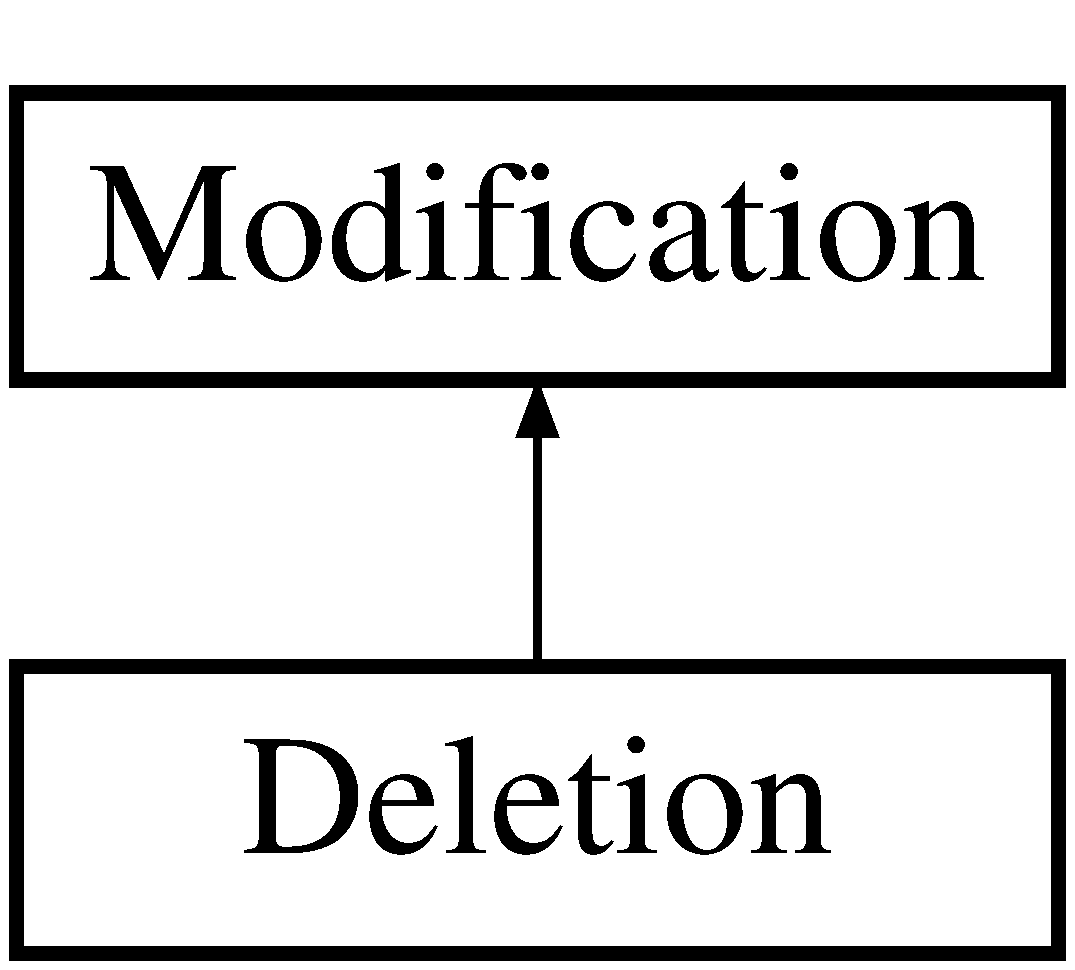
\includegraphics[height=2.000000cm]{class_deletion}
\end{center}
\end{figure}
\subsection*{Public Member Functions}
\begin{DoxyCompactItemize}
\item 
\mbox{\hyperlink{class_deletion_a8446318e3f7004ef557b6021350fa389}{Deletion}} (\mbox{\hyperlink{class_tree_object}{Tree\+Object}} $\ast$obj, \mbox{\hyperlink{class_tree_object}{Tree\+Object}} $\ast$parent)
\item 
\mbox{\hyperlink{class_deletion_ad56d54e1ab5d4d2a875b6093c05ba1d8}{$\sim$\+Deletion}} ()
\item 
void \mbox{\hyperlink{class_deletion_ac5bdb21c4a8dbc8afea9910435e509a8}{write\+\_\+out}} (\mbox{\hyperlink{class_partition_manager}{Partition\+Manager}} $\ast$pm)
\end{DoxyCompactItemize}
\subsection*{Additional Inherited Members}


\subsection{Constructor \& Destructor Documentation}
\mbox{\Hypertarget{class_deletion_a8446318e3f7004ef557b6021350fa389}\label{class_deletion_a8446318e3f7004ef557b6021350fa389}} 
\index{Deletion@{Deletion}!Deletion@{Deletion}}
\index{Deletion@{Deletion}!Deletion@{Deletion}}
\subsubsection{\texorpdfstring{Deletion()}{Deletion()}}
{\footnotesize\ttfamily Deletion\+::\+Deletion (\begin{DoxyParamCaption}\item[{\mbox{\hyperlink{class_tree_object}{Tree\+Object}} $\ast$}]{obj,  }\item[{\mbox{\hyperlink{class_tree_object}{Tree\+Object}} $\ast$}]{parent }\end{DoxyParamCaption})}

\mbox{\Hypertarget{class_deletion_ad56d54e1ab5d4d2a875b6093c05ba1d8}\label{class_deletion_ad56d54e1ab5d4d2a875b6093c05ba1d8}} 
\index{Deletion@{Deletion}!````~Deletion@{$\sim$\+Deletion}}
\index{````~Deletion@{$\sim$\+Deletion}!Deletion@{Deletion}}
\subsubsection{\texorpdfstring{$\sim$\+Deletion()}{~Deletion()}}
{\footnotesize\ttfamily Deletion\+::$\sim$\+Deletion (\begin{DoxyParamCaption}{ }\end{DoxyParamCaption})}



\subsection{Member Function Documentation}
\mbox{\Hypertarget{class_deletion_ac5bdb21c4a8dbc8afea9910435e509a8}\label{class_deletion_ac5bdb21c4a8dbc8afea9910435e509a8}} 
\index{Deletion@{Deletion}!write\+\_\+out@{write\+\_\+out}}
\index{write\+\_\+out@{write\+\_\+out}!Deletion@{Deletion}}
\subsubsection{\texorpdfstring{write\+\_\+out()}{write\_out()}}
{\footnotesize\ttfamily void Deletion\+::write\+\_\+out (\begin{DoxyParamCaption}\item[{\mbox{\hyperlink{class_partition_manager}{Partition\+Manager}} $\ast$}]{pm }\end{DoxyParamCaption})\hspace{0.3cm}{\ttfamily [virtual]}}



Implements \mbox{\hyperlink{class_modification_a50d1fd809524902d2a1e78d02f4be1dc}{Modification}}.



The documentation for this class was generated from the following files\+:\begin{DoxyCompactItemize}
\item 
Filesystem/\+Daemon\+Dependancies/\+Trees/\mbox{\hyperlink{_trees_8h}{Trees.\+h}}\item 
Filesystem/\+Daemon\+Dependancies/\+Trees/\mbox{\hyperlink{_trees_8cpp}{Trees.\+cpp}}\end{DoxyCompactItemize}

\hypertarget{class_disk}{}\section{Disk Class Reference}
\label{class_disk}\index{Disk@{Disk}}


{\ttfamily \#include $<$Disk.\+h$>$}

\subsection*{Public Member Functions}
\begin{DoxyCompactItemize}
\item 
\mbox{\hyperlink{class_disk_a5be49d1002da046d1890df1b088900e4}{Disk}} (Blk\+Num\+Type numblocks, size\+\_\+t block\+Size, char $\ast$location)
\item 
\mbox{\hyperlink{class_disk_a77518c808f3f5d9e902a55942542c337}{$\sim$\+Disk}} ()
\end{DoxyCompactItemize}
\begin{Indent}\textbf{ Modifier Functions}\par
\begin{DoxyCompactItemize}
\item 
void \mbox{\hyperlink{class_disk_a5d335138f56e6b87c8ebc4b6473183e7}{write\+Disk\+Block}} (Blk\+Num\+Type blknum, char $\ast$blkdata)
\end{DoxyCompactItemize}
\end{Indent}
\begin{Indent}\textbf{ Accessor Functions}\par
\begin{DoxyCompactItemize}
\item 
void \mbox{\hyperlink{class_disk_a2598cdd9013bdbb1213afa878c567daa}{read\+Disk\+Block}} (Blk\+Num\+Type blknum, char $\ast$blkdata)
\item 
size\+\_\+t \mbox{\hyperlink{class_disk_a1c149b57524fe4e7ae7c8643309e0501}{get\+Block\+Size}} ()
\item 
int \mbox{\hyperlink{class_disk_a3c61119ce5707dd4ab039201590a7c22}{get\+Block\+Count}} ()
\end{DoxyCompactItemize}
\end{Indent}
\subsection*{Private Attributes}
\begin{DoxyCompactItemize}
\item 
Blk\+Num\+Type \mbox{\hyperlink{class_disk_a6389ea8f99ad557d02685b292c23a656}{\+\_\+disk\+Size}}
\item 
size\+\_\+t \mbox{\hyperlink{class_disk_a3207de813954dad3e2547c7a892a04a7}{\+\_\+block\+Size}}
\item 
Blk\+Num\+Type \mbox{\hyperlink{class_disk_a35a2900e2a8d3b567ef7280d3c475eac}{\+\_\+block\+Count}}
\item 
char $\ast$ \mbox{\hyperlink{class_disk_a04bd92b804d0c07e87a9277fa647c972}{\+\_\+disk\+Location}}
\end{DoxyCompactItemize}


\subsection{Constructor \& Destructor Documentation}
\mbox{\Hypertarget{class_disk_a5be49d1002da046d1890df1b088900e4}\label{class_disk_a5be49d1002da046d1890df1b088900e4}} 
\index{Disk@{Disk}!Disk@{Disk}}
\index{Disk@{Disk}!Disk@{Disk}}
\subsubsection{\texorpdfstring{Disk()}{Disk()}}
{\footnotesize\ttfamily Disk\+::\+Disk (\begin{DoxyParamCaption}\item[{Blk\+Num\+Type}]{numblocks,  }\item[{size\+\_\+t}]{block\+Size,  }\item[{char $\ast$}]{location }\end{DoxyParamCaption})}


\begin{DoxyParams}{Parameters}
{\em numblocks} & the number of blocks on the \mbox{\hyperlink{class_disk}{Disk}} \\
\hline
{\em blocksize} & the block size for \mbox{\hyperlink{class_disk}{Disk}} blocks \\
\hline
{\em location} & the location of the \mbox{\hyperlink{class_disk}{Disk}} \\
\hline
\end{DoxyParams}
\mbox{\Hypertarget{class_disk_a77518c808f3f5d9e902a55942542c337}\label{class_disk_a77518c808f3f5d9e902a55942542c337}} 
\index{Disk@{Disk}!````~Disk@{$\sim$\+Disk}}
\index{````~Disk@{$\sim$\+Disk}!Disk@{Disk}}
\subsubsection{\texorpdfstring{$\sim$\+Disk()}{~Disk()}}
{\footnotesize\ttfamily Disk\+::$\sim$\+Disk (\begin{DoxyParamCaption}{ }\end{DoxyParamCaption})}



\subsection{Member Function Documentation}
\mbox{\Hypertarget{class_disk_a3c61119ce5707dd4ab039201590a7c22}\label{class_disk_a3c61119ce5707dd4ab039201590a7c22}} 
\index{Disk@{Disk}!get\+Block\+Count@{get\+Block\+Count}}
\index{get\+Block\+Count@{get\+Block\+Count}!Disk@{Disk}}
\subsubsection{\texorpdfstring{get\+Block\+Count()}{getBlockCount()}}
{\footnotesize\ttfamily int Disk\+::get\+Block\+Count (\begin{DoxyParamCaption}{ }\end{DoxyParamCaption})}

\begin{DoxyReturn}{Returns}
the number of blocks on the entire \mbox{\hyperlink{class_disk}{Disk}} 
\end{DoxyReturn}
\mbox{\Hypertarget{class_disk_a1c149b57524fe4e7ae7c8643309e0501}\label{class_disk_a1c149b57524fe4e7ae7c8643309e0501}} 
\index{Disk@{Disk}!get\+Block\+Size@{get\+Block\+Size}}
\index{get\+Block\+Size@{get\+Block\+Size}!Disk@{Disk}}
\subsubsection{\texorpdfstring{get\+Block\+Size()}{getBlockSize()}}
{\footnotesize\ttfamily size\+\_\+t Disk\+::get\+Block\+Size (\begin{DoxyParamCaption}{ }\end{DoxyParamCaption})}

\begin{DoxyReturn}{Returns}
the blocksize of the \mbox{\hyperlink{class_disk}{Disk}} 
\end{DoxyReturn}
\mbox{\Hypertarget{class_disk_a2598cdd9013bdbb1213afa878c567daa}\label{class_disk_a2598cdd9013bdbb1213afa878c567daa}} 
\index{Disk@{Disk}!read\+Disk\+Block@{read\+Disk\+Block}}
\index{read\+Disk\+Block@{read\+Disk\+Block}!Disk@{Disk}}
\subsubsection{\texorpdfstring{read\+Disk\+Block()}{readDiskBlock()}}
{\footnotesize\ttfamily void Disk\+::read\+Disk\+Block (\begin{DoxyParamCaption}\item[{Blk\+Num\+Type}]{blknum,  }\item[{char $\ast$}]{blkdata }\end{DoxyParamCaption})}

Reads a block from the \mbox{\hyperlink{class_disk}{Disk}}. 
\begin{DoxyParams}{Parameters}
{\em blknum} & the blocknumber to be read \\
\hline
{\em blkdata} & the buffer to put the read data. must be large enough to contain an entire block of data \\
\hline
\end{DoxyParams}
\begin{DoxySeeAlso}{See also}
Partition\+Manger\+::read\+Disk\+Block() Parition\+Manager\+::read\+Disk\+Block() 
\end{DoxySeeAlso}
\mbox{\Hypertarget{class_disk_a5d335138f56e6b87c8ebc4b6473183e7}\label{class_disk_a5d335138f56e6b87c8ebc4b6473183e7}} 
\index{Disk@{Disk}!write\+Disk\+Block@{write\+Disk\+Block}}
\index{write\+Disk\+Block@{write\+Disk\+Block}!Disk@{Disk}}
\subsubsection{\texorpdfstring{write\+Disk\+Block()}{writeDiskBlock()}}
{\footnotesize\ttfamily void Disk\+::write\+Disk\+Block (\begin{DoxyParamCaption}\item[{Blk\+Num\+Type}]{blknum,  }\item[{char $\ast$}]{blkdata }\end{DoxyParamCaption})}

Writes a block to the \mbox{\hyperlink{class_disk}{Disk}}. 
\begin{DoxyParams}{Parameters}
{\em blknum} & the blocknumber to be written \\
\hline
{\em blkdata} & the buffer to write the data from. It Will write an entire block size of data. \\
\hline
\end{DoxyParams}
\begin{DoxySeeAlso}{See also}
Partition\+Manger\+::write\+Disk\+Block() Parition\+Manager\+::write\+Disk\+Block() 
\end{DoxySeeAlso}


\subsection{Member Data Documentation}
\mbox{\Hypertarget{class_disk_a35a2900e2a8d3b567ef7280d3c475eac}\label{class_disk_a35a2900e2a8d3b567ef7280d3c475eac}} 
\index{Disk@{Disk}!\+\_\+block\+Count@{\+\_\+block\+Count}}
\index{\+\_\+block\+Count@{\+\_\+block\+Count}!Disk@{Disk}}
\subsubsection{\texorpdfstring{\+\_\+block\+Count}{\_blockCount}}
{\footnotesize\ttfamily Blk\+Num\+Type Disk\+::\+\_\+block\+Count\hspace{0.3cm}{\ttfamily [private]}}

\mbox{\Hypertarget{class_disk_a3207de813954dad3e2547c7a892a04a7}\label{class_disk_a3207de813954dad3e2547c7a892a04a7}} 
\index{Disk@{Disk}!\+\_\+block\+Size@{\+\_\+block\+Size}}
\index{\+\_\+block\+Size@{\+\_\+block\+Size}!Disk@{Disk}}
\subsubsection{\texorpdfstring{\+\_\+block\+Size}{\_blockSize}}
{\footnotesize\ttfamily size\+\_\+t Disk\+::\+\_\+block\+Size\hspace{0.3cm}{\ttfamily [private]}}

\mbox{\Hypertarget{class_disk_a04bd92b804d0c07e87a9277fa647c972}\label{class_disk_a04bd92b804d0c07e87a9277fa647c972}} 
\index{Disk@{Disk}!\+\_\+disk\+Location@{\+\_\+disk\+Location}}
\index{\+\_\+disk\+Location@{\+\_\+disk\+Location}!Disk@{Disk}}
\subsubsection{\texorpdfstring{\+\_\+disk\+Location}{\_diskLocation}}
{\footnotesize\ttfamily char$\ast$ Disk\+::\+\_\+disk\+Location\hspace{0.3cm}{\ttfamily [private]}}

\mbox{\Hypertarget{class_disk_a6389ea8f99ad557d02685b292c23a656}\label{class_disk_a6389ea8f99ad557d02685b292c23a656}} 
\index{Disk@{Disk}!\+\_\+disk\+Size@{\+\_\+disk\+Size}}
\index{\+\_\+disk\+Size@{\+\_\+disk\+Size}!Disk@{Disk}}
\subsubsection{\texorpdfstring{\+\_\+disk\+Size}{\_diskSize}}
{\footnotesize\ttfamily Blk\+Num\+Type Disk\+::\+\_\+disk\+Size\hspace{0.3cm}{\ttfamily [private]}}



The documentation for this class was generated from the following files\+:\begin{DoxyCompactItemize}
\item 
Filesystem/\+Daemon\+Dependancies/\+Disk/\mbox{\hyperlink{_disk_8h}{Disk.\+h}}\item 
Filesystem/\+Daemon\+Dependancies/\+Disk/\mbox{\hyperlink{_disk_8cpp}{Disk.\+cpp}}\end{DoxyCompactItemize}

\hypertarget{classdisk__error}{}\section{disk\+\_\+error Class Reference}
\label{classdisk__error}\index{disk\+\_\+error@{disk\+\_\+error}}
Inheritance diagram for disk\+\_\+error\+:\begin{figure}[H]
\begin{center}
\leavevmode
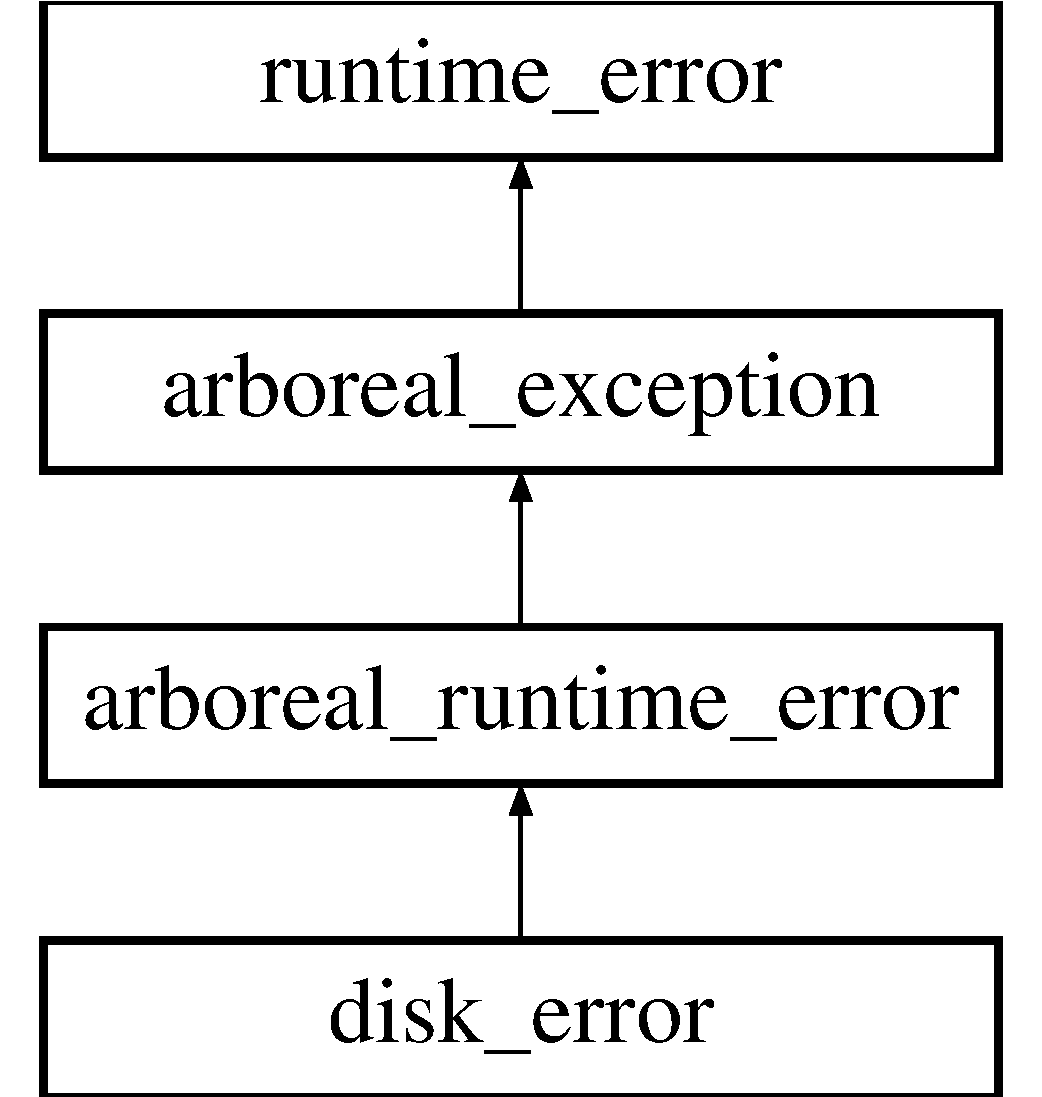
\includegraphics[height=4.000000cm]{classdisk__error}
\end{center}
\end{figure}
\subsection*{Public Member Functions}
\begin{DoxyCompactItemize}
\item 
\mbox{\Hypertarget{classdisk__error_a1f3a9f8326a8d192d3a54e698d09d29d}\label{classdisk__error_a1f3a9f8326a8d192d3a54e698d09d29d}} 
{\bfseries disk\+\_\+error} (const char $\ast$what, const char $\ast$where)
\item 
\mbox{\Hypertarget{classdisk__error_a03937aabd05ba77b2e49fff4c039b047}\label{classdisk__error_a03937aabd05ba77b2e49fff4c039b047}} 
{\bfseries disk\+\_\+error} (const char $\ast$what, const string \&where)
\item 
\mbox{\Hypertarget{classdisk__error_afb8e69ac35d47d5ed1bcc8b764baea4b}\label{classdisk__error_afb8e69ac35d47d5ed1bcc8b764baea4b}} 
{\bfseries disk\+\_\+error} (const string \&what, const string \&where)
\item 
\mbox{\Hypertarget{classdisk__error_aea5a9df17b57607f55f82de0cd384052}\label{classdisk__error_aea5a9df17b57607f55f82de0cd384052}} 
{\bfseries disk\+\_\+error} (const string \&what, const char $\ast$where)
\end{DoxyCompactItemize}
\subsection*{Additional Inherited Members}


The documentation for this class was generated from the following files\+:\begin{DoxyCompactItemize}
\item 
Filesystem/Arboreal\+\_\+\+Exceptions.\+h\item 
Filesystem/Arboreal\+\_\+\+Exceptions.\+cpp\end{DoxyCompactItemize}

\hypertarget{class_disk_manager}{}\section{Disk\+Manager Class Reference}
\label{class_disk_manager}\index{Disk\+Manager@{Disk\+Manager}}


{\ttfamily \#include $<$Disk\+Manager.\+h$>$}

\subsection*{Public Member Functions}
\begin{DoxyCompactItemize}
\item 
\mbox{\hyperlink{class_disk_manager_a948cecec230d9895bafaced5534fd6cf}{Disk\+Manager}} (\mbox{\hyperlink{class_disk}{Disk}} $\ast$\mbox{\hyperlink{daemon_8h_a86c4a7377e8e3575bcce3c81a810d503}{d}})
\item 
\mbox{\hyperlink{class_disk_manager_a60837a3b8064649adf23e3143c85aed7}{$\sim$\+Disk\+Manager}} ()
\end{DoxyCompactItemize}
\begin{Indent}\textbf{ Accessor Functions}\par
\begin{DoxyCompactItemize}
\item 
void \mbox{\hyperlink{class_disk_manager_afda24be04fb85711236a4d5905a5ad1c}{read\+Disk\+Block}} (string partition\+Name, Blk\+Num\+Type blknum, char $\ast$blkdata)
\item 
size\+\_\+t \mbox{\hyperlink{class_disk_manager_aabdfbb2171f3c19a3ae14f9532876404}{get\+Block\+Size}} ()
\item 
Blk\+Num\+Type \mbox{\hyperlink{class_disk_manager_ae32627ccfa72013e35da637570e1729b}{get\+Partition\+Size}} (string partition\+Name)
\item 
\mbox{\hyperlink{struct_disk_partition}{Disk\+Partition}} $\ast$ \mbox{\hyperlink{class_disk_manager_a08375c254bc09c8351a4f96cb669f1ab}{find\+Part}} (string partition\+Name)
\end{DoxyCompactItemize}
\end{Indent}
\begin{Indent}\textbf{ Modifier Functions}\par
\begin{DoxyCompactItemize}
\item 
void \mbox{\hyperlink{class_disk_manager_ac96846d309a59e8ac7b100724329cb30}{write\+Disk\+Block}} (string partition\+Name, Blk\+Num\+Type blknum, char $\ast$blkdata)
\end{DoxyCompactItemize}
\end{Indent}
\subsection*{Private Attributes}
\begin{DoxyCompactItemize}
\item 
\mbox{\hyperlink{class_disk}{Disk}} $\ast$ \mbox{\hyperlink{class_disk_manager_a2f342673f450be650f1b08650b6b6e40}{\+\_\+my\+Disk}}
\item 
vector$<$ \mbox{\hyperlink{struct_disk_partition}{Disk\+Partition}} $\ast$ $>$ \mbox{\hyperlink{class_disk_manager_ae509fd85f802b1dcab2368a146b17ae7}{\+\_\+my\+Partitions}}
\end{DoxyCompactItemize}


\subsection{Constructor \& Destructor Documentation}
\mbox{\Hypertarget{class_disk_manager_a948cecec230d9895bafaced5534fd6cf}\label{class_disk_manager_a948cecec230d9895bafaced5534fd6cf}} 
\index{Disk\+Manager@{Disk\+Manager}!Disk\+Manager@{Disk\+Manager}}
\index{Disk\+Manager@{Disk\+Manager}!Disk\+Manager@{Disk\+Manager}}
\subsubsection{\texorpdfstring{Disk\+Manager()}{DiskManager()}}
{\footnotesize\ttfamily Disk\+Manager\+::\+Disk\+Manager (\begin{DoxyParamCaption}\item[{\mbox{\hyperlink{class_disk}{Disk}} $\ast$}]{d }\end{DoxyParamCaption})}


\begin{DoxyParams}{Parameters}
{\em d} & Pointer to the \mbox{\hyperlink{class_disk}{Disk}} this will manage \\
\hline
\end{DoxyParams}
\mbox{\Hypertarget{class_disk_manager_a60837a3b8064649adf23e3143c85aed7}\label{class_disk_manager_a60837a3b8064649adf23e3143c85aed7}} 
\index{Disk\+Manager@{Disk\+Manager}!````~Disk\+Manager@{$\sim$\+Disk\+Manager}}
\index{````~Disk\+Manager@{$\sim$\+Disk\+Manager}!Disk\+Manager@{Disk\+Manager}}
\subsubsection{\texorpdfstring{$\sim$\+Disk\+Manager()}{~DiskManager()}}
{\footnotesize\ttfamily Disk\+Manager\+::$\sim$\+Disk\+Manager (\begin{DoxyParamCaption}{ }\end{DoxyParamCaption})}



\subsection{Member Function Documentation}
\mbox{\Hypertarget{class_disk_manager_a08375c254bc09c8351a4f96cb669f1ab}\label{class_disk_manager_a08375c254bc09c8351a4f96cb669f1ab}} 
\index{Disk\+Manager@{Disk\+Manager}!find\+Part@{find\+Part}}
\index{find\+Part@{find\+Part}!Disk\+Manager@{Disk\+Manager}}
\subsubsection{\texorpdfstring{find\+Part()}{findPart()}}
{\footnotesize\ttfamily \mbox{\hyperlink{struct_disk_partition}{Disk\+Partition}} $\ast$ Disk\+Manager\+::find\+Part (\begin{DoxyParamCaption}\item[{string}]{partition\+Name }\end{DoxyParamCaption})}


\begin{DoxyParams}{Parameters}
{\em partition\+Name} & the name of the partition \\
\hline
\end{DoxyParams}
\begin{DoxyReturn}{Returns}
the size of a partition in blocks 
\end{DoxyReturn}
\mbox{\Hypertarget{class_disk_manager_aabdfbb2171f3c19a3ae14f9532876404}\label{class_disk_manager_aabdfbb2171f3c19a3ae14f9532876404}} 
\index{Disk\+Manager@{Disk\+Manager}!get\+Block\+Size@{get\+Block\+Size}}
\index{get\+Block\+Size@{get\+Block\+Size}!Disk\+Manager@{Disk\+Manager}}
\subsubsection{\texorpdfstring{get\+Block\+Size()}{getBlockSize()}}
{\footnotesize\ttfamily size\+\_\+t Disk\+Manager\+::get\+Block\+Size (\begin{DoxyParamCaption}{ }\end{DoxyParamCaption})}

\begin{DoxyReturn}{Returns}
the blocksize of the \mbox{\hyperlink{class_disk}{Disk}} 
\end{DoxyReturn}
\mbox{\Hypertarget{class_disk_manager_ae32627ccfa72013e35da637570e1729b}\label{class_disk_manager_ae32627ccfa72013e35da637570e1729b}} 
\index{Disk\+Manager@{Disk\+Manager}!get\+Partition\+Size@{get\+Partition\+Size}}
\index{get\+Partition\+Size@{get\+Partition\+Size}!Disk\+Manager@{Disk\+Manager}}
\subsubsection{\texorpdfstring{get\+Partition\+Size()}{getPartitionSize()}}
{\footnotesize\ttfamily Blk\+Num\+Type Disk\+Manager\+::get\+Partition\+Size (\begin{DoxyParamCaption}\item[{string}]{partition\+Name }\end{DoxyParamCaption})}


\begin{DoxyParams}{Parameters}
{\em partition\+Name} & the name of the partition \\
\hline
\end{DoxyParams}
\begin{DoxyReturn}{Returns}
the size of a partition in blocks 
\end{DoxyReturn}
\mbox{\Hypertarget{class_disk_manager_afda24be04fb85711236a4d5905a5ad1c}\label{class_disk_manager_afda24be04fb85711236a4d5905a5ad1c}} 
\index{Disk\+Manager@{Disk\+Manager}!read\+Disk\+Block@{read\+Disk\+Block}}
\index{read\+Disk\+Block@{read\+Disk\+Block}!Disk\+Manager@{Disk\+Manager}}
\subsubsection{\texorpdfstring{read\+Disk\+Block()}{readDiskBlock()}}
{\footnotesize\ttfamily void Disk\+Manager\+::read\+Disk\+Block (\begin{DoxyParamCaption}\item[{string}]{partition\+Name,  }\item[{Blk\+Num\+Type}]{blknum,  }\item[{char $\ast$}]{blkdata }\end{DoxyParamCaption})}

Reads a block from the \mbox{\hyperlink{class_disk}{Disk}}. 
\begin{DoxyParams}{Parameters}
{\em partition\+Name} & the name of the partition to write the block to \\
\hline
{\em blknum} & the blocknumber to be read \\
\hline
{\em blkdata} & the buffer to put the read data. must be large enough to contain an entire block of data \\
\hline
\end{DoxyParams}
\begin{DoxySeeAlso}{See also}
Partition\+Manger\+::read\+Disk\+Block() Parition\+Manager\+::read\+Disk\+Block() 
\end{DoxySeeAlso}
\mbox{\Hypertarget{class_disk_manager_ac96846d309a59e8ac7b100724329cb30}\label{class_disk_manager_ac96846d309a59e8ac7b100724329cb30}} 
\index{Disk\+Manager@{Disk\+Manager}!write\+Disk\+Block@{write\+Disk\+Block}}
\index{write\+Disk\+Block@{write\+Disk\+Block}!Disk\+Manager@{Disk\+Manager}}
\subsubsection{\texorpdfstring{write\+Disk\+Block()}{writeDiskBlock()}}
{\footnotesize\ttfamily void Disk\+Manager\+::write\+Disk\+Block (\begin{DoxyParamCaption}\item[{string}]{partition\+Name,  }\item[{Blk\+Num\+Type}]{blknum,  }\item[{char $\ast$}]{blkdata }\end{DoxyParamCaption})}

Writes a block to the \mbox{\hyperlink{class_disk}{Disk}}. 
\begin{DoxyParams}{Parameters}
{\em partition\+Name} & the name of the partition to write the block to \\
\hline
{\em blknum} & the blocknumber to be written \\
\hline
{\em blkdata} & the buffer to write the data from. It Will write an entire block size of data. \\
\hline
\end{DoxyParams}
\begin{DoxySeeAlso}{See also}
Partition\+Manger\+::write\+Disk\+Block() Parition\+Manager\+::write\+Disk\+Block() 
\end{DoxySeeAlso}


\subsection{Member Data Documentation}
\mbox{\Hypertarget{class_disk_manager_a2f342673f450be650f1b08650b6b6e40}\label{class_disk_manager_a2f342673f450be650f1b08650b6b6e40}} 
\index{Disk\+Manager@{Disk\+Manager}!\+\_\+my\+Disk@{\+\_\+my\+Disk}}
\index{\+\_\+my\+Disk@{\+\_\+my\+Disk}!Disk\+Manager@{Disk\+Manager}}
\subsubsection{\texorpdfstring{\+\_\+my\+Disk}{\_myDisk}}
{\footnotesize\ttfamily \mbox{\hyperlink{class_disk}{Disk}}$\ast$ Disk\+Manager\+::\+\_\+my\+Disk\hspace{0.3cm}{\ttfamily [private]}}

\mbox{\Hypertarget{class_disk_manager_ae509fd85f802b1dcab2368a146b17ae7}\label{class_disk_manager_ae509fd85f802b1dcab2368a146b17ae7}} 
\index{Disk\+Manager@{Disk\+Manager}!\+\_\+my\+Partitions@{\+\_\+my\+Partitions}}
\index{\+\_\+my\+Partitions@{\+\_\+my\+Partitions}!Disk\+Manager@{Disk\+Manager}}
\subsubsection{\texorpdfstring{\+\_\+my\+Partitions}{\_myPartitions}}
{\footnotesize\ttfamily vector$<$\mbox{\hyperlink{struct_disk_partition}{Disk\+Partition}}$\ast$$>$ Disk\+Manager\+::\+\_\+my\+Partitions\hspace{0.3cm}{\ttfamily [private]}}



The documentation for this class was generated from the following files\+:\begin{DoxyCompactItemize}
\item 
Filesystem/\+Daemon\+Dependancies/\+Disk\+Manager/\mbox{\hyperlink{_disk_manager_8h}{Disk\+Manager.\+h}}\item 
Filesystem/\+Daemon\+Dependancies/\+Disk\+Manager/\mbox{\hyperlink{_disk_manager_8cpp}{Disk\+Manager.\+cpp}}\end{DoxyCompactItemize}

\hypertarget{struct_disk_partition}{}\section{Disk\+Partition Struct Reference}
\label{struct_disk_partition}\index{Disk\+Partition@{Disk\+Partition}}


{\ttfamily \#include $<$Disk\+Manager.\+h$>$}

\subsection*{Public Attributes}
\begin{DoxyCompactItemize}
\item 
string \mbox{\hyperlink{struct_disk_partition_a8c89b5f115fa534a3cb5d76505de97cb}{partition\+Name}}
\item 
Blk\+Num\+Type \mbox{\hyperlink{struct_disk_partition_a61dfe31b8baf361738168c2521c19286}{partition\+Size}}
\item 
Blk\+Num\+Type \mbox{\hyperlink{struct_disk_partition_a2b5b89e7739ffa6ac21772a92f88e35f}{partition\+Blk\+Start}}
\item 
int \mbox{\hyperlink{struct_disk_partition_a6fd44394d9d8bf83fa61cfd12be25412}{file\+Name\+Size}}
\end{DoxyCompactItemize}


\subsection{Member Data Documentation}
\mbox{\Hypertarget{struct_disk_partition_a6fd44394d9d8bf83fa61cfd12be25412}\label{struct_disk_partition_a6fd44394d9d8bf83fa61cfd12be25412}} 
\index{Disk\+Partition@{Disk\+Partition}!file\+Name\+Size@{file\+Name\+Size}}
\index{file\+Name\+Size@{file\+Name\+Size}!Disk\+Partition@{Disk\+Partition}}
\subsubsection{\texorpdfstring{file\+Name\+Size}{fileNameSize}}
{\footnotesize\ttfamily int Disk\+Partition\+::file\+Name\+Size}

\mbox{\Hypertarget{struct_disk_partition_a2b5b89e7739ffa6ac21772a92f88e35f}\label{struct_disk_partition_a2b5b89e7739ffa6ac21772a92f88e35f}} 
\index{Disk\+Partition@{Disk\+Partition}!partition\+Blk\+Start@{partition\+Blk\+Start}}
\index{partition\+Blk\+Start@{partition\+Blk\+Start}!Disk\+Partition@{Disk\+Partition}}
\subsubsection{\texorpdfstring{partition\+Blk\+Start}{partitionBlkStart}}
{\footnotesize\ttfamily Blk\+Num\+Type Disk\+Partition\+::partition\+Blk\+Start}

\mbox{\Hypertarget{struct_disk_partition_a8c89b5f115fa534a3cb5d76505de97cb}\label{struct_disk_partition_a8c89b5f115fa534a3cb5d76505de97cb}} 
\index{Disk\+Partition@{Disk\+Partition}!partition\+Name@{partition\+Name}}
\index{partition\+Name@{partition\+Name}!Disk\+Partition@{Disk\+Partition}}
\subsubsection{\texorpdfstring{partition\+Name}{partitionName}}
{\footnotesize\ttfamily string Disk\+Partition\+::partition\+Name}

\mbox{\Hypertarget{struct_disk_partition_a61dfe31b8baf361738168c2521c19286}\label{struct_disk_partition_a61dfe31b8baf361738168c2521c19286}} 
\index{Disk\+Partition@{Disk\+Partition}!partition\+Size@{partition\+Size}}
\index{partition\+Size@{partition\+Size}!Disk\+Partition@{Disk\+Partition}}
\subsubsection{\texorpdfstring{partition\+Size}{partitionSize}}
{\footnotesize\ttfamily Blk\+Num\+Type Disk\+Partition\+::partition\+Size}



The documentation for this struct was generated from the following file\+:\begin{DoxyCompactItemize}
\item 
Filesystem/\+Daemon\+Dependancies/\+Disk\+Manager/\mbox{\hyperlink{_disk_manager_8h}{Disk\+Manager.\+h}}\end{DoxyCompactItemize}

\hypertarget{class_file}{}\section{File Class Reference}
\label{class_file}\index{File@{File}}


{\ttfamily \#include $<$File.\+h$>$}

\subsection*{Public Member Functions}
\begin{DoxyCompactItemize}
\item 
\mbox{\hyperlink{class_file_af29e498f601951f4ccf06f2fc3fb1f73}{File}} (string name, const vector$<$ string $>$ \&tags, File\+Attributes attributes)
\end{DoxyCompactItemize}
\begin{Indent}\textbf{ Accessor Functions}\par
\begin{DoxyCompactItemize}
\item 
string \mbox{\hyperlink{class_file_a4b8e86f4fae0219744cf82f6bab35b53}{get\+\_\+name}} ()
\item 
vector$<$ string $>$ \& \mbox{\hyperlink{class_file_a479270bfe1fa436d317151ac108eb28a}{get\+\_\+tags}} ()
\item 
File\+Attributes \mbox{\hyperlink{class_file_a9f59d3d546e8e574889558d63c71bf02}{get\+\_\+attributes}} ()
\end{DoxyCompactItemize}
\end{Indent}
\subsection*{Static Public Member Functions}
\begin{DoxyCompactItemize}
\item 
static \mbox{\hyperlink{class_file}{File}} $\ast$ \mbox{\hyperlink{class_file_a1118d477e6b00d789e948e8cca5ae393}{read\+\_\+buff}} (const char $\ast$serialized\+File)
\end{DoxyCompactItemize}
\subsection*{Private Attributes}
\begin{DoxyCompactItemize}
\item 
string \mbox{\hyperlink{class_file_a9668b6d84f8f57a737e30d87f08725cd}{\+\_\+name}}
\item 
File\+Attributes \mbox{\hyperlink{class_file_ae2faf26750f73c5848cf414f208282b2}{\+\_\+attributes}}
\item 
vector$<$ string $>$ \mbox{\hyperlink{class_file_aa4bc599b81fee53fd7b7b9d7f8129e11}{\+\_\+tags}}
\end{DoxyCompactItemize}


\subsection{Constructor \& Destructor Documentation}
\mbox{\Hypertarget{class_file_af29e498f601951f4ccf06f2fc3fb1f73}\label{class_file_af29e498f601951f4ccf06f2fc3fb1f73}} 
\index{File@{File}!File@{File}}
\index{File@{File}!File@{File}}
\subsubsection{\texorpdfstring{File()}{File()}}
{\footnotesize\ttfamily File\+::\+File (\begin{DoxyParamCaption}\item[{string}]{name,  }\item[{const vector$<$ string $>$ \&}]{tags,  }\item[{File\+Attributes}]{attributes }\end{DoxyParamCaption})}


\begin{DoxyParams}{Parameters}
{\em name} & the name of the \mbox{\hyperlink{class_file}{File}} \\
\hline
{\em tags} & the tags to be associated with the \mbox{\hyperlink{class_file}{File}} \\
\hline
{\em attributes} & the \mbox{\hyperlink{class_file}{File}} attributes \\
\hline
\end{DoxyParams}


\subsection{Member Function Documentation}
\mbox{\Hypertarget{class_file_a9f59d3d546e8e574889558d63c71bf02}\label{class_file_a9f59d3d546e8e574889558d63c71bf02}} 
\index{File@{File}!get\+\_\+attributes@{get\+\_\+attributes}}
\index{get\+\_\+attributes@{get\+\_\+attributes}!File@{File}}
\subsubsection{\texorpdfstring{get\+\_\+attributes()}{get\_attributes()}}
{\footnotesize\ttfamily File\+Attributes File\+::get\+\_\+attributes (\begin{DoxyParamCaption}{ }\end{DoxyParamCaption})}

\begin{DoxyReturn}{Returns}
the attributes associated with this \mbox{\hyperlink{class_file}{File}} 
\end{DoxyReturn}
\mbox{\Hypertarget{class_file_a4b8e86f4fae0219744cf82f6bab35b53}\label{class_file_a4b8e86f4fae0219744cf82f6bab35b53}} 
\index{File@{File}!get\+\_\+name@{get\+\_\+name}}
\index{get\+\_\+name@{get\+\_\+name}!File@{File}}
\subsubsection{\texorpdfstring{get\+\_\+name()}{get\_name()}}
{\footnotesize\ttfamily string File\+::get\+\_\+name (\begin{DoxyParamCaption}{ }\end{DoxyParamCaption})}

\begin{DoxyReturn}{Returns}
The name of the \mbox{\hyperlink{class_file}{File}} 
\end{DoxyReturn}
\mbox{\Hypertarget{class_file_a479270bfe1fa436d317151ac108eb28a}\label{class_file_a479270bfe1fa436d317151ac108eb28a}} 
\index{File@{File}!get\+\_\+tags@{get\+\_\+tags}}
\index{get\+\_\+tags@{get\+\_\+tags}!File@{File}}
\subsubsection{\texorpdfstring{get\+\_\+tags()}{get\_tags()}}
{\footnotesize\ttfamily vector$<$ string $>$ \& File\+::get\+\_\+tags (\begin{DoxyParamCaption}{ }\end{DoxyParamCaption})}

\begin{DoxyReturn}{Returns}
The tags associated with this \mbox{\hyperlink{class_file}{File}} 
\end{DoxyReturn}
\mbox{\Hypertarget{class_file_a1118d477e6b00d789e948e8cca5ae393}\label{class_file_a1118d477e6b00d789e948e8cca5ae393}} 
\index{File@{File}!read\+\_\+buff@{read\+\_\+buff}}
\index{read\+\_\+buff@{read\+\_\+buff}!File@{File}}
\subsubsection{\texorpdfstring{read\+\_\+buff()}{read\_buff()}}
{\footnotesize\ttfamily \mbox{\hyperlink{class_file}{File}} $\ast$ File\+::read\+\_\+buff (\begin{DoxyParamCaption}\item[{const char $\ast$}]{serialized\+File }\end{DoxyParamCaption})\hspace{0.3cm}{\ttfamily [static]}}

Will take a char$\ast$ buffer and create a \mbox{\hyperlink{class_file}{File}} object from it. The buffer must have been serialized in the correct format 
\begin{DoxyParams}{Parameters}
{\em serialized\+File} & the serialized\+File object \\
\hline
\end{DoxyParams}
\begin{DoxyReturn}{Returns}
a File$\ast$ to the created \mbox{\hyperlink{class_file}{File}} 
\end{DoxyReturn}
\begin{DoxySeeAlso}{See also}
\mbox{\hyperlink{class_file_info_a64fc62c3e376dfd61088932d8b793589}{File\+Info\+::serialize()}} 
\end{DoxySeeAlso}


\subsection{Member Data Documentation}
\mbox{\Hypertarget{class_file_ae2faf26750f73c5848cf414f208282b2}\label{class_file_ae2faf26750f73c5848cf414f208282b2}} 
\index{File@{File}!\+\_\+attributes@{\+\_\+attributes}}
\index{\+\_\+attributes@{\+\_\+attributes}!File@{File}}
\subsubsection{\texorpdfstring{\+\_\+attributes}{\_attributes}}
{\footnotesize\ttfamily File\+Attributes File\+::\+\_\+attributes\hspace{0.3cm}{\ttfamily [private]}}

\mbox{\Hypertarget{class_file_a9668b6d84f8f57a737e30d87f08725cd}\label{class_file_a9668b6d84f8f57a737e30d87f08725cd}} 
\index{File@{File}!\+\_\+name@{\+\_\+name}}
\index{\+\_\+name@{\+\_\+name}!File@{File}}
\subsubsection{\texorpdfstring{\+\_\+name}{\_name}}
{\footnotesize\ttfamily string File\+::\+\_\+name\hspace{0.3cm}{\ttfamily [private]}}

\mbox{\Hypertarget{class_file_aa4bc599b81fee53fd7b7b9d7f8129e11}\label{class_file_aa4bc599b81fee53fd7b7b9d7f8129e11}} 
\index{File@{File}!\+\_\+tags@{\+\_\+tags}}
\index{\+\_\+tags@{\+\_\+tags}!File@{File}}
\subsubsection{\texorpdfstring{\+\_\+tags}{\_tags}}
{\footnotesize\ttfamily vector$<$string$>$ File\+::\+\_\+tags\hspace{0.3cm}{\ttfamily [private]}}



The documentation for this class was generated from the following files\+:\begin{DoxyCompactItemize}
\item 
Filesystem/\+Daemon\+Dependancies/\+File/\mbox{\hyperlink{_file_8h}{File.\+h}}\item 
Filesystem/\+Daemon\+Dependancies/\+File/\mbox{\hyperlink{_file_8cpp}{File.\+cpp}}\end{DoxyCompactItemize}

\hypertarget{classfile__error}{}\section{file\+\_\+error Class Reference}
\label{classfile__error}\index{file\+\_\+error@{file\+\_\+error}}
Inheritance diagram for file\+\_\+error\+:\begin{figure}[H]
\begin{center}
\leavevmode
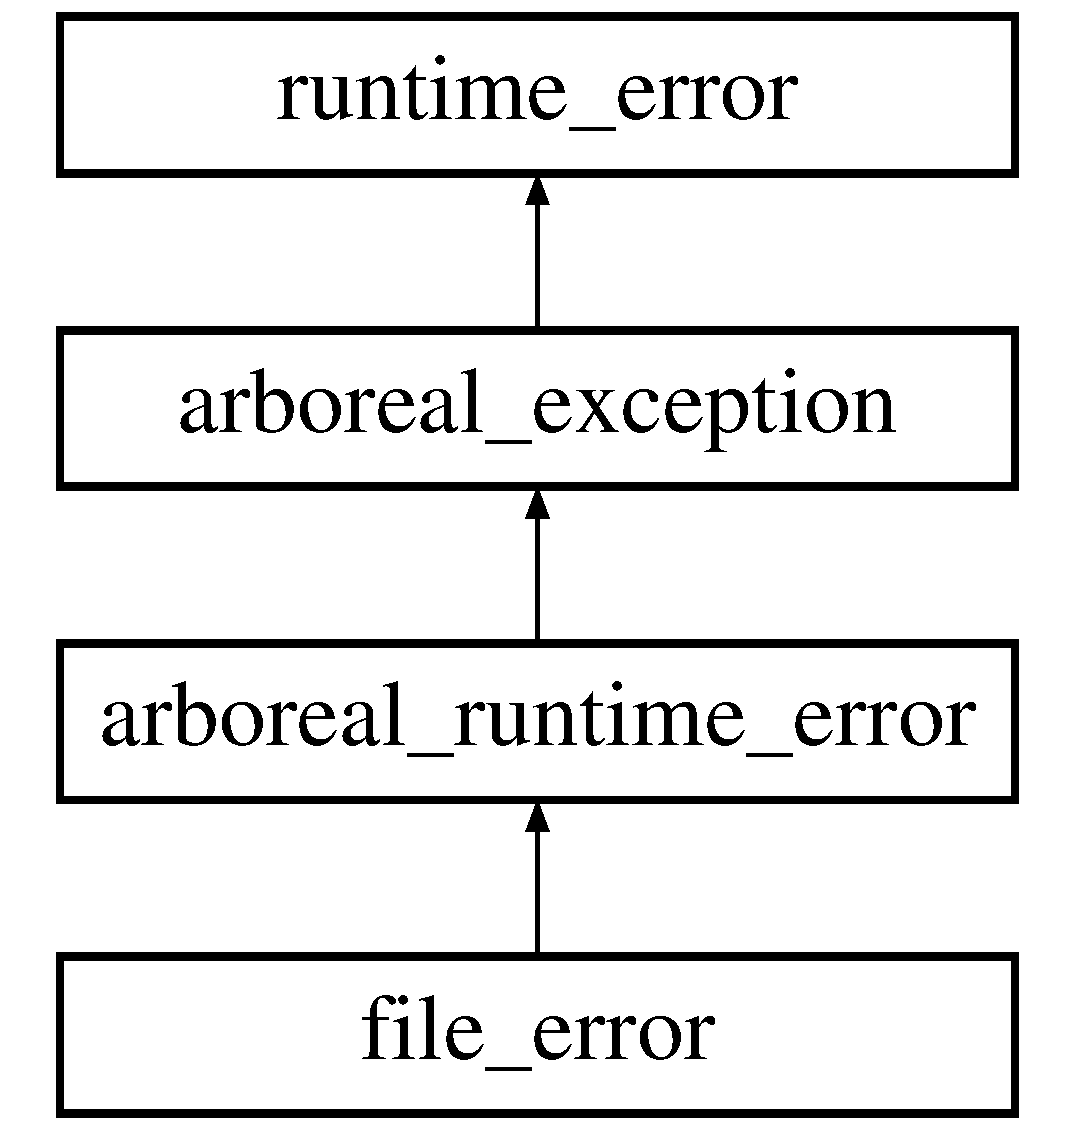
\includegraphics[height=4.000000cm]{db/ddf/classfile__error}
\end{center}
\end{figure}
\subsection*{Public Member Functions}
\begin{DoxyCompactItemize}
\item 
\mbox{\Hypertarget{classfile__error_a10da41c5d15b25fdafa97ae79523e242}\label{classfile__error_a10da41c5d15b25fdafa97ae79523e242}} 
{\bfseries file\+\_\+error} (const char $\ast$what, const char $\ast$where, const int ecode=99)
\item 
\mbox{\Hypertarget{classfile__error_ae70ca16a0a8eee95a88a64128b7fcbad}\label{classfile__error_ae70ca16a0a8eee95a88a64128b7fcbad}} 
{\bfseries file\+\_\+error} (const char $\ast$what, const string \&where, const int ecode=99)
\item 
\mbox{\Hypertarget{classfile__error_a9b1c03f989df972ca3201f984ddece6d}\label{classfile__error_a9b1c03f989df972ca3201f984ddece6d}} 
{\bfseries file\+\_\+error} (const string \&what, const string \&where, const int ecode=99)
\item 
\mbox{\Hypertarget{classfile__error_a2698ca75c20dd3ffc5adb8d470fff246}\label{classfile__error_a2698ca75c20dd3ffc5adb8d470fff246}} 
{\bfseries file\+\_\+error} (const string \&what, const char $\ast$where, const int ecode=99)
\end{DoxyCompactItemize}
\subsection*{Additional Inherited Members}


The documentation for this class was generated from the following files\+:\begin{DoxyCompactItemize}
\item 
Shared\+Headers/Arboreal\+\_\+\+Exceptions.\+h\item 
Shared\+C\+P\+P\+Files/Arboreal\+\_\+\+Exceptions.\+cpp\end{DoxyCompactItemize}

\hypertarget{class_file_info}{}\section{File\+Info Class Reference}
\label{class_file_info}\index{File\+Info@{File\+Info}}


{\ttfamily \#include $<$Trees.\+h$>$}

Inheritance diagram for File\+Info\+:\begin{figure}[H]
\begin{center}
\leavevmode
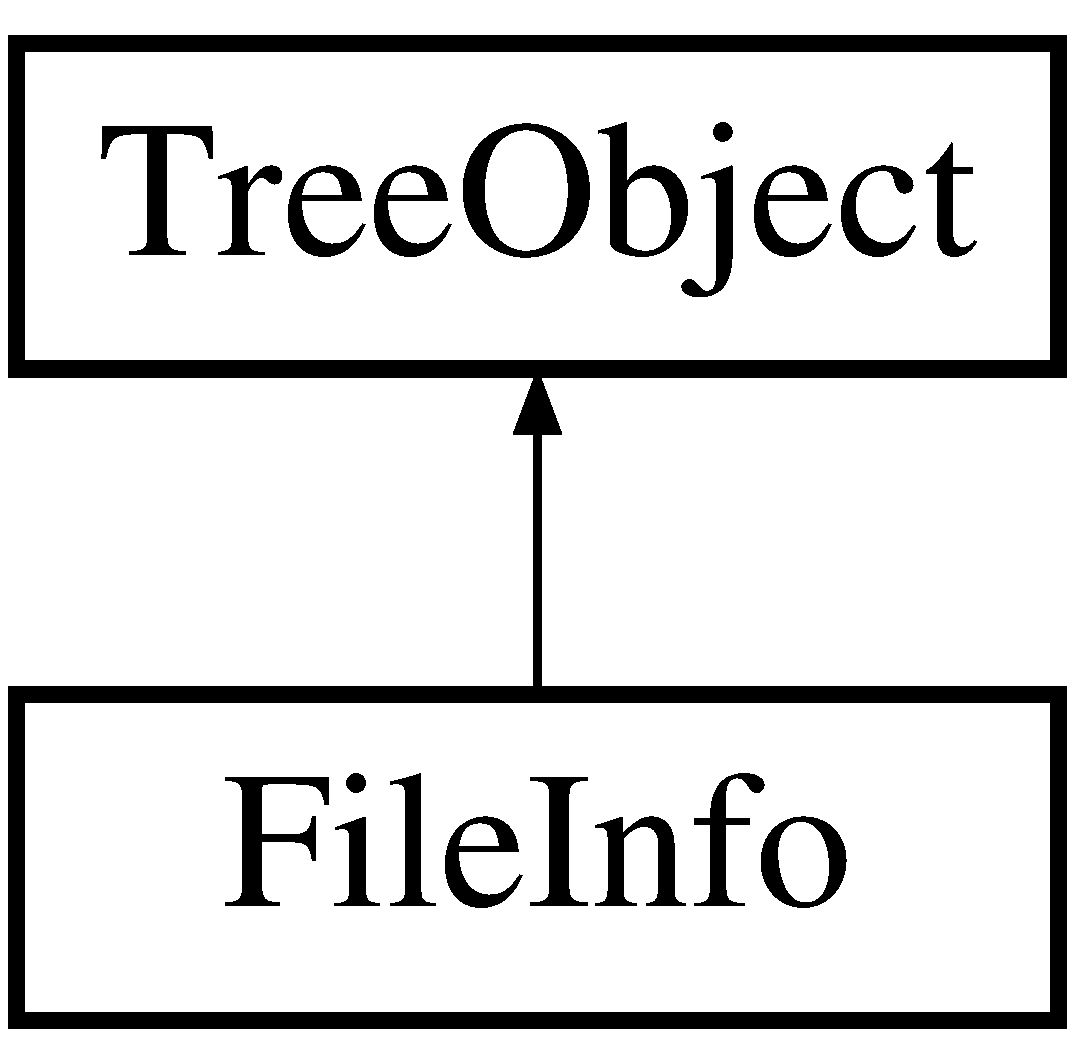
\includegraphics[height=2.000000cm]{class_file_info}
\end{center}
\end{figure}
\subsection*{Public Member Functions}
\begin{DoxyCompactItemize}
\item 
\mbox{\hyperlink{class_file_info_a3586bb4f50c4a0f63ff4ea0a1e56ce9c}{File\+Info}} (string filename, Blk\+Num\+Type blknum, \mbox{\hyperlink{class_partition_manager}{Partition\+Manager}} $\ast$pm)
\item 
\mbox{\hyperlink{class_file_info_ab771dfaca29680c93810af82a7a99958}{$\sim$\+File\+Info}} ()
\item 
void \mbox{\hyperlink{class_file_info_a8e835f000ddfd0f1097ccfa7e7801a09}{write\+\_\+out}} ()
\item 
void \mbox{\hyperlink{class_file_info_a2bf60d4be97347f3d7a15cf839afca7d}{read\+\_\+in}} (unordered\+\_\+multimap$<$ string, \mbox{\hyperlink{class_file_info}{File\+Info}} $\ast$$>$ $\ast$all\+Files, \mbox{\hyperlink{class_root_tree}{Root\+Tree}} $\ast$root\+Tree)
\item 
void \mbox{\hyperlink{class_file_info_ae058242283d3317eaf2b79428e6137f6}{erase}} (string name)
\item 
void \mbox{\hyperlink{class_file_info_ad93a84b63e417b07aa68b619051ab746}{insert}} (string name, \mbox{\hyperlink{class_tree_object}{Tree\+Object}} $\ast$ptr)
\item 
void \mbox{\hyperlink{class_file_info_a2ca34d945ed1208f227a249ba72ee427}{del}} ()
\item 
void \mbox{\hyperlink{class_file_info_a8c6b58cb9f7e9978064291ef81380e01}{delete\+\_\+cont\+\_\+blocks}} (Blk\+Num\+Type blknum)
\item 
void \mbox{\hyperlink{class_file_info_a7f788f31521c535646eebfa9959bbb24}{insert\+\_\+addition}} (\mbox{\hyperlink{class_tree_object}{Tree\+Object}} $\ast$add)
\item 
void \mbox{\hyperlink{class_file_info_a278136b1d68f55dc56a4be807076fc0d}{insert\+\_\+deletion}} (\mbox{\hyperlink{class_tree_object}{Tree\+Object}} $\ast$\mbox{\hyperlink{class_file_info_a2ca34d945ed1208f227a249ba72ee427}{del}})
\end{DoxyCompactItemize}
\begin{Indent}\textbf{ Accessor Functions}\par
\begin{DoxyCompactItemize}
\item 
string \mbox{\hyperlink{class_file_info_a96827c2e48fb1a15d468e9afd545383e}{mangle}} ()
\begin{DoxyCompactList}\small\item\em mangles the filename with its tags \end{DoxyCompactList}\item 
string \mbox{\hyperlink{class_file_info_a105ad751f21bead6fc2a76e79cb3b701}{mangle}} (vector$<$ string $>$ \&tags)
\begin{DoxyCompactList}\small\item\em mangles the filename with the specified tags \end{DoxyCompactList}\item 
string \mbox{\hyperlink{class_file_info_aec8a60addbed54097f6cac0a6a516717}{mangle}} (unordered\+\_\+set$<$ string $>$ \&tags)
\begin{DoxyCompactList}\small\item\em mangles the filename with the specified tags \end{DoxyCompactList}\item 
Finode \mbox{\hyperlink{class_file_info_a706117270bcf31739d7ce0aa0d79891f}{get\+\_\+finode}} ()
\item 
size\+\_\+t \mbox{\hyperlink{class_file_info_aa07a5b95bfd41814b7fb2ee30a279c65}{get\+\_\+file\+\_\+size}} ()
\item 
\mbox{\hyperlink{class_attributes}{Attributes}} $\ast$ \mbox{\hyperlink{class_file_info_a07f09582ef3c3beb105906d5c71234a5}{get\+\_\+attributes}} ()
\item 
unordered\+\_\+set$<$ string $>$ \mbox{\hyperlink{class_file_info_a63d01334c1c2ae22e5d1930afa5c74d4}{get\+\_\+tags}} ()
\end{DoxyCompactItemize}
\end{Indent}
\begin{Indent}\textbf{ Modifier Functions}\par
\begin{DoxyCompactItemize}
\item 
void \mbox{\hyperlink{class_file_info_a1537d2ac2b5c170d144911c8337c81bc}{add\+\_\+direct\+\_\+block}} (Blk\+Num\+Type blknum, int index)
\item 
void \mbox{\hyperlink{class_file_info_a074956f43b5a6900205a541dbeaeb8c5}{add\+\_\+indirect\+\_\+block}} (Blk\+Num\+Type blknum, short level)
\item 
void \mbox{\hyperlink{class_file_info_a3c548a8dfcb6530bfef7551ac24ca473}{update\+\_\+file\+\_\+size}} (size\+\_\+t bytes)
\item 
void \mbox{\hyperlink{class_file_info_aacaeadeeb41726f8cbea0b7cb1ff6a22}{set\+\_\+access}} ()
\item 
void \mbox{\hyperlink{class_file_info_a05eb10c6804660ecd47e556c27ecd019}{set\+\_\+edit}} ()
\item 
void \mbox{\hyperlink{class_file_info_a377208012195dba0b24723837f6db39f}{set\+\_\+permissions}} (char $\ast$perms)
\begin{DoxyCompactList}\small\item\em sets the permisssions for this file \end{DoxyCompactList}\end{DoxyCompactItemize}
\end{Indent}
\subsection*{Static Public Member Functions}
\begin{DoxyCompactItemize}
\item 
static string $\ast$ \mbox{\hyperlink{class_file_info_a64fc62c3e376dfd61088932d8b793589}{serialize}} (\mbox{\hyperlink{class_file_info}{File\+Info}} $\ast$file)
\end{DoxyCompactItemize}
\subsection*{Private Member Functions}
\begin{DoxyCompactItemize}
\item 
void \mbox{\hyperlink{class_file_info_abad45da4fbc2f1da564a23a2c3e6caff}{init\+\_\+attributes}} ()
\end{DoxyCompactItemize}
\subsection*{Private Attributes}
\begin{DoxyCompactItemize}
\item 
\mbox{\hyperlink{class_attributes}{Attributes}} $\ast$ \mbox{\hyperlink{class_file_info_ad074cd1ea6b131fe01d7bd18a9da7230}{\+\_\+my\+Attributes}}
\item 
Finode \mbox{\hyperlink{class_file_info_aa9f9a75407d29778170a902e070d47ad}{\+\_\+my\+Finode}}
\end{DoxyCompactItemize}
\subsection*{Additional Inherited Members}


\subsection{Constructor \& Destructor Documentation}
\mbox{\Hypertarget{class_file_info_a3586bb4f50c4a0f63ff4ea0a1e56ce9c}\label{class_file_info_a3586bb4f50c4a0f63ff4ea0a1e56ce9c}} 
\index{File\+Info@{File\+Info}!File\+Info@{File\+Info}}
\index{File\+Info@{File\+Info}!File\+Info@{File\+Info}}
\subsubsection{\texorpdfstring{File\+Info()}{FileInfo()}}
{\footnotesize\ttfamily File\+Info\+::\+File\+Info (\begin{DoxyParamCaption}\item[{string}]{filename,  }\item[{Blk\+Num\+Type}]{blknum,  }\item[{\mbox{\hyperlink{class_partition_manager}{Partition\+Manager}} $\ast$}]{pm }\end{DoxyParamCaption})}


\begin{DoxyParams}{Parameters}
{\em filename} & Name of the \mbox{\hyperlink{class_file}{File}} \\
\hline
{\em blknum} & the blocknumber of the associated Finode on disk \\
\hline
\end{DoxyParams}
\mbox{\Hypertarget{class_file_info_ab771dfaca29680c93810af82a7a99958}\label{class_file_info_ab771dfaca29680c93810af82a7a99958}} 
\index{File\+Info@{File\+Info}!````~File\+Info@{$\sim$\+File\+Info}}
\index{````~File\+Info@{$\sim$\+File\+Info}!File\+Info@{File\+Info}}
\subsubsection{\texorpdfstring{$\sim$\+File\+Info()}{~FileInfo()}}
{\footnotesize\ttfamily File\+Info\+::$\sim$\+File\+Info (\begin{DoxyParamCaption}{ }\end{DoxyParamCaption})}



\subsection{Member Function Documentation}
\mbox{\Hypertarget{class_file_info_a1537d2ac2b5c170d144911c8337c81bc}\label{class_file_info_a1537d2ac2b5c170d144911c8337c81bc}} 
\index{File\+Info@{File\+Info}!add\+\_\+direct\+\_\+block@{add\+\_\+direct\+\_\+block}}
\index{add\+\_\+direct\+\_\+block@{add\+\_\+direct\+\_\+block}!File\+Info@{File\+Info}}
\subsubsection{\texorpdfstring{add\+\_\+direct\+\_\+block()}{add\_direct\_block()}}
{\footnotesize\ttfamily void File\+Info\+::add\+\_\+direct\+\_\+block (\begin{DoxyParamCaption}\item[{Blk\+Num\+Type}]{blknum,  }\item[{int}]{index }\end{DoxyParamCaption})}

adds the specified blocknumber to the array of direct blocks in this file\textquotesingle{}s Finode 
\begin{DoxyParams}{Parameters}
{\em blknum} & the block number of the direct block that has already been allocated \\
\hline
{\em index} & the index of the blknum in the array, must be less than 12 and at least 0. \\
\hline
\end{DoxyParams}

\begin{DoxyExceptions}{Exceptions}
{\em \mbox{\hyperlink{classarboreal__logic__error}{arboreal\+\_\+logic\+\_\+error}}} & index out of bounds \\
\hline
\end{DoxyExceptions}
\begin{DoxySeeAlso}{See also}
\mbox{\hyperlink{class_file_info_a074956f43b5a6900205a541dbeaeb8c5}{add\+\_\+indirect\+\_\+block}} 
\end{DoxySeeAlso}
\mbox{\Hypertarget{class_file_info_a074956f43b5a6900205a541dbeaeb8c5}\label{class_file_info_a074956f43b5a6900205a541dbeaeb8c5}} 
\index{File\+Info@{File\+Info}!add\+\_\+indirect\+\_\+block@{add\+\_\+indirect\+\_\+block}}
\index{add\+\_\+indirect\+\_\+block@{add\+\_\+indirect\+\_\+block}!File\+Info@{File\+Info}}
\subsubsection{\texorpdfstring{add\+\_\+indirect\+\_\+block()}{add\_indirect\_block()}}
{\footnotesize\ttfamily void File\+Info\+::add\+\_\+indirect\+\_\+block (\begin{DoxyParamCaption}\item[{Blk\+Num\+Type}]{blknum,  }\item[{short}]{level }\end{DoxyParamCaption})}

adds the specified blocknumber to the Finode as the start of the specified level of indirect blocks 
\begin{DoxyParams}{Parameters}
{\em blknum} & the block number of the indirect block that has already been allocated \\
\hline
{\em level} & the level that the block number is associated with. must be 1, 2 or 3. \\
\hline
\end{DoxyParams}

\begin{DoxyExceptions}{Exceptions}
{\em \mbox{\hyperlink{classarboreal__logic__error}{arboreal\+\_\+logic\+\_\+error}}} & Invalid level \\
\hline
\end{DoxyExceptions}
\begin{DoxySeeAlso}{See also}
\mbox{\hyperlink{class_file_info_a1537d2ac2b5c170d144911c8337c81bc}{add\+\_\+direct\+\_\+block}} 
\end{DoxySeeAlso}
\mbox{\Hypertarget{class_file_info_a2ca34d945ed1208f227a249ba72ee427}\label{class_file_info_a2ca34d945ed1208f227a249ba72ee427}} 
\index{File\+Info@{File\+Info}!del@{del}}
\index{del@{del}!File\+Info@{File\+Info}}
\subsubsection{\texorpdfstring{del()}{del()}}
{\footnotesize\ttfamily void File\+Info\+::del (\begin{DoxyParamCaption}{ }\end{DoxyParamCaption})\hspace{0.3cm}{\ttfamily [virtual]}}

Will completely remove the \mbox{\hyperlink{class_tree_object}{Tree\+Object}}\textquotesingle{}s presence on disk 

Implements \mbox{\hyperlink{class_tree_object_af390b7479aa972888e594c07a85740b6}{Tree\+Object}}.

\mbox{\Hypertarget{class_file_info_a8c6b58cb9f7e9978064291ef81380e01}\label{class_file_info_a8c6b58cb9f7e9978064291ef81380e01}} 
\index{File\+Info@{File\+Info}!delete\+\_\+cont\+\_\+blocks@{delete\+\_\+cont\+\_\+blocks}}
\index{delete\+\_\+cont\+\_\+blocks@{delete\+\_\+cont\+\_\+blocks}!File\+Info@{File\+Info}}
\subsubsection{\texorpdfstring{delete\+\_\+cont\+\_\+blocks()}{delete\_cont\_blocks()}}
{\footnotesize\ttfamily void File\+Info\+::delete\+\_\+cont\+\_\+blocks (\begin{DoxyParamCaption}\item[{Blk\+Num\+Type}]{blknum }\end{DoxyParamCaption})\hspace{0.3cm}{\ttfamily [virtual]}}

Will follow the chain of continuation blocks and free all of them 
\begin{DoxyParams}{Parameters}
{\em blknum} & will free the blknum and use it to follow the chain of continuation blocks \\
\hline
\end{DoxyParams}


Reimplemented from \mbox{\hyperlink{class_tree_object_a07f5f5de1cff0cfdc2372e81559f5181}{Tree\+Object}}.

\mbox{\Hypertarget{class_file_info_ae058242283d3317eaf2b79428e6137f6}\label{class_file_info_ae058242283d3317eaf2b79428e6137f6}} 
\index{File\+Info@{File\+Info}!erase@{erase}}
\index{erase@{erase}!File\+Info@{File\+Info}}
\subsubsection{\texorpdfstring{erase()}{erase()}}
{\footnotesize\ttfamily void File\+Info\+::erase (\begin{DoxyParamCaption}\item[{string}]{name }\end{DoxyParamCaption})\hspace{0.3cm}{\ttfamily [virtual]}}

Disassociate the given name from this object 
\begin{DoxyParams}{Parameters}
{\em name} & the name of the object to be erased. \\
\hline
\end{DoxyParams}

\begin{DoxyExceptions}{Exceptions}
{\em \mbox{\hyperlink{classarboreal__logic__error}{arboreal\+\_\+logic\+\_\+error}}} & \\
\hline
\end{DoxyExceptions}


Reimplemented from \mbox{\hyperlink{class_tree_object_a453b5df2a9ef7c6faad259900d574ee2}{Tree\+Object}}.

\mbox{\Hypertarget{class_file_info_a07f09582ef3c3beb105906d5c71234a5}\label{class_file_info_a07f09582ef3c3beb105906d5c71234a5}} 
\index{File\+Info@{File\+Info}!get\+\_\+attributes@{get\+\_\+attributes}}
\index{get\+\_\+attributes@{get\+\_\+attributes}!File\+Info@{File\+Info}}
\subsubsection{\texorpdfstring{get\+\_\+attributes()}{get\_attributes()}}
{\footnotesize\ttfamily \mbox{\hyperlink{class_attributes}{Attributes}} $\ast$ File\+Info\+::get\+\_\+attributes (\begin{DoxyParamCaption}{ }\end{DoxyParamCaption})}

\begin{DoxyReturn}{Returns}
the \mbox{\hyperlink{class_attributes}{Attributes}} accociated with this file 
\end{DoxyReturn}
\mbox{\Hypertarget{class_file_info_aa07a5b95bfd41814b7fb2ee30a279c65}\label{class_file_info_aa07a5b95bfd41814b7fb2ee30a279c65}} 
\index{File\+Info@{File\+Info}!get\+\_\+file\+\_\+size@{get\+\_\+file\+\_\+size}}
\index{get\+\_\+file\+\_\+size@{get\+\_\+file\+\_\+size}!File\+Info@{File\+Info}}
\subsubsection{\texorpdfstring{get\+\_\+file\+\_\+size()}{get\_file\_size()}}
{\footnotesize\ttfamily size\+\_\+t File\+Info\+::get\+\_\+file\+\_\+size (\begin{DoxyParamCaption}{ }\end{DoxyParamCaption})}

\begin{DoxyReturn}{Returns}
the size of this file in bytes 
\end{DoxyReturn}
\mbox{\Hypertarget{class_file_info_a706117270bcf31739d7ce0aa0d79891f}\label{class_file_info_a706117270bcf31739d7ce0aa0d79891f}} 
\index{File\+Info@{File\+Info}!get\+\_\+finode@{get\+\_\+finode}}
\index{get\+\_\+finode@{get\+\_\+finode}!File\+Info@{File\+Info}}
\subsubsection{\texorpdfstring{get\+\_\+finode()}{get\_finode()}}
{\footnotesize\ttfamily Finode File\+Info\+::get\+\_\+finode (\begin{DoxyParamCaption}{ }\end{DoxyParamCaption})}

\begin{DoxyReturn}{Returns}
the Finode associated with this file 
\end{DoxyReturn}
\mbox{\Hypertarget{class_file_info_a63d01334c1c2ae22e5d1930afa5c74d4}\label{class_file_info_a63d01334c1c2ae22e5d1930afa5c74d4}} 
\index{File\+Info@{File\+Info}!get\+\_\+tags@{get\+\_\+tags}}
\index{get\+\_\+tags@{get\+\_\+tags}!File\+Info@{File\+Info}}
\subsubsection{\texorpdfstring{get\+\_\+tags()}{get\_tags()}}
{\footnotesize\ttfamily unordered\+\_\+set$<$ string $>$ File\+Info\+::get\+\_\+tags (\begin{DoxyParamCaption}{ }\end{DoxyParamCaption})}

\begin{DoxyReturn}{Returns}
The tags associated with this file 
\end{DoxyReturn}
\mbox{\Hypertarget{class_file_info_abad45da4fbc2f1da564a23a2c3e6caff}\label{class_file_info_abad45da4fbc2f1da564a23a2c3e6caff}} 
\index{File\+Info@{File\+Info}!init\+\_\+attributes@{init\+\_\+attributes}}
\index{init\+\_\+attributes@{init\+\_\+attributes}!File\+Info@{File\+Info}}
\subsubsection{\texorpdfstring{init\+\_\+attributes()}{init\_attributes()}}
{\footnotesize\ttfamily void File\+Info\+::init\+\_\+attributes (\begin{DoxyParamCaption}{ }\end{DoxyParamCaption})\hspace{0.3cm}{\ttfamily [private]}}

\mbox{\Hypertarget{class_file_info_ad93a84b63e417b07aa68b619051ab746}\label{class_file_info_ad93a84b63e417b07aa68b619051ab746}} 
\index{File\+Info@{File\+Info}!insert@{insert}}
\index{insert@{insert}!File\+Info@{File\+Info}}
\subsubsection{\texorpdfstring{insert()}{insert()}}
{\footnotesize\ttfamily void File\+Info\+::insert (\begin{DoxyParamCaption}\item[{string}]{name,  }\item[{\mbox{\hyperlink{class_tree_object}{Tree\+Object}} $\ast$}]{obj }\end{DoxyParamCaption})\hspace{0.3cm}{\ttfamily [virtual]}}

Associate a \mbox{\hyperlink{class_tree_object}{Tree\+Object}} with this object 
\begin{DoxyParams}{Parameters}
{\em name} & name of the object, mangled if inserting a \mbox{\hyperlink{class_file_info}{File\+Info}} \\
\hline
{\em obj} & the object to be inserted \\
\hline
\end{DoxyParams}

\begin{DoxyExceptions}{Exceptions}
{\em \mbox{\hyperlink{classtag__error}{tag\+\_\+error}}} & \\
\hline
\end{DoxyExceptions}
\begin{DoxySeeAlso}{See also}
\mbox{\hyperlink{class_file_info_ad93a84b63e417b07aa68b619051ab746}{File\+Info\+::insert()}} 
\end{DoxySeeAlso}


Reimplemented from \mbox{\hyperlink{class_tree_object_af8cc57edba9f435b52ccf33cfbbb2fc6}{Tree\+Object}}.

\mbox{\Hypertarget{class_file_info_a7f788f31521c535646eebfa9959bbb24}\label{class_file_info_a7f788f31521c535646eebfa9959bbb24}} 
\index{File\+Info@{File\+Info}!insert\+\_\+addition@{insert\+\_\+addition}}
\index{insert\+\_\+addition@{insert\+\_\+addition}!File\+Info@{File\+Info}}
\subsubsection{\texorpdfstring{insert\+\_\+addition()}{insert\_addition()}}
{\footnotesize\ttfamily void File\+Info\+::insert\+\_\+addition (\begin{DoxyParamCaption}\item[{\mbox{\hyperlink{class_tree_object}{Tree\+Object}} $\ast$}]{add }\end{DoxyParamCaption})\hspace{0.3cm}{\ttfamily [virtual]}}

Do not call on \mbox{\hyperlink{class_file_info}{File\+Info}} 

Reimplemented from \mbox{\hyperlink{class_tree_object_a41ce6080e0df5adcea4b0a76d35af885}{Tree\+Object}}.

\mbox{\Hypertarget{class_file_info_a278136b1d68f55dc56a4be807076fc0d}\label{class_file_info_a278136b1d68f55dc56a4be807076fc0d}} 
\index{File\+Info@{File\+Info}!insert\+\_\+deletion@{insert\+\_\+deletion}}
\index{insert\+\_\+deletion@{insert\+\_\+deletion}!File\+Info@{File\+Info}}
\subsubsection{\texorpdfstring{insert\+\_\+deletion()}{insert\_deletion()}}
{\footnotesize\ttfamily void File\+Info\+::insert\+\_\+deletion (\begin{DoxyParamCaption}\item[{\mbox{\hyperlink{class_tree_object}{Tree\+Object}} $\ast$}]{del }\end{DoxyParamCaption})\hspace{0.3cm}{\ttfamily [virtual]}}

Do not call on \mbox{\hyperlink{class_file_info}{File\+Info}} 

Reimplemented from \mbox{\hyperlink{class_tree_object_afcc4b3928d2b77ff080aa229a9706215}{Tree\+Object}}.

\mbox{\Hypertarget{class_file_info_a96827c2e48fb1a15d468e9afd545383e}\label{class_file_info_a96827c2e48fb1a15d468e9afd545383e}} 
\index{File\+Info@{File\+Info}!mangle@{mangle}}
\index{mangle@{mangle}!File\+Info@{File\+Info}}
\subsubsection{\texorpdfstring{mangle()}{mangle()}\hspace{0.1cm}{\footnotesize\ttfamily [1/3]}}
{\footnotesize\ttfamily string File\+Info\+::mangle (\begin{DoxyParamCaption}{ }\end{DoxyParamCaption})}



mangles the filename with its tags 

The name is mangled as follows\+: Each tag is placed in alphabetical order and appended to the filename using \textquotesingle{}\+\_\+\textquotesingle{} as the seperator.

\begin{DoxyReturn}{Returns}
the mangled name of this file. 
\end{DoxyReturn}
\begin{DoxySeeAlso}{See also}
\mbox{\hyperlink{class_file_info_a105ad751f21bead6fc2a76e79cb3b701}{mangle(vector$<$string$>$\&)}} \mbox{\hyperlink{class_file_info_aec8a60addbed54097f6cac0a6a516717}{mangle(unordered\+\_\+set$<$string$>$\& tags)}} 
\end{DoxySeeAlso}
\mbox{\Hypertarget{class_file_info_a105ad751f21bead6fc2a76e79cb3b701}\label{class_file_info_a105ad751f21bead6fc2a76e79cb3b701}} 
\index{File\+Info@{File\+Info}!mangle@{mangle}}
\index{mangle@{mangle}!File\+Info@{File\+Info}}
\subsubsection{\texorpdfstring{mangle()}{mangle()}\hspace{0.1cm}{\footnotesize\ttfamily [2/3]}}
{\footnotesize\ttfamily string File\+Info\+::mangle (\begin{DoxyParamCaption}\item[{vector$<$ string $>$ \&}]{tags }\end{DoxyParamCaption})}



mangles the filename with the specified tags 

The name is mangled as follows\+: Each tag is placed in alphabetical order and appended to the filename using \textquotesingle{}\+\_\+\textquotesingle{} as the seperator. \begin{DoxyReturn}{Returns}
the mangled name of this file. 
\end{DoxyReturn}

\begin{DoxyParams}{Parameters}
{\em tags} & the tags you wish to mangle the filename with \\
\hline
\end{DoxyParams}
\begin{DoxySeeAlso}{See also}
\mbox{\hyperlink{class_file_info_a96827c2e48fb1a15d468e9afd545383e}{mangle()}} \mbox{\hyperlink{class_file_info_aec8a60addbed54097f6cac0a6a516717}{mangle(unordered\+\_\+set$<$string$>$\& tags)}} 
\end{DoxySeeAlso}
\mbox{\Hypertarget{class_file_info_aec8a60addbed54097f6cac0a6a516717}\label{class_file_info_aec8a60addbed54097f6cac0a6a516717}} 
\index{File\+Info@{File\+Info}!mangle@{mangle}}
\index{mangle@{mangle}!File\+Info@{File\+Info}}
\subsubsection{\texorpdfstring{mangle()}{mangle()}\hspace{0.1cm}{\footnotesize\ttfamily [3/3]}}
{\footnotesize\ttfamily string File\+Info\+::mangle (\begin{DoxyParamCaption}\item[{unordered\+\_\+set$<$ string $>$ \&}]{tags }\end{DoxyParamCaption})}



mangles the filename with the specified tags 

) The name is mangled as follows\+: Each tag is placed in alphabetical order and appended to the filename using \textquotesingle{}\+\_\+\textquotesingle{} as the seperator.

\begin{DoxyReturn}{Returns}
the mangled name of this file. 
\end{DoxyReturn}

\begin{DoxyParams}{Parameters}
{\em tags} & the tags you wish to mangle the filename with \\
\hline
\end{DoxyParams}
\begin{DoxySeeAlso}{See also}
\mbox{\hyperlink{class_file_info_a96827c2e48fb1a15d468e9afd545383e}{mangle()}} \mbox{\hyperlink{class_file_info_a96827c2e48fb1a15d468e9afd545383e}{mangle}}(unordered\+\_\+set$<$string$>$\& tags 
\end{DoxySeeAlso}
\mbox{\Hypertarget{class_file_info_a2bf60d4be97347f3d7a15cf839afca7d}\label{class_file_info_a2bf60d4be97347f3d7a15cf839afca7d}} 
\index{File\+Info@{File\+Info}!read\+\_\+in@{read\+\_\+in}}
\index{read\+\_\+in@{read\+\_\+in}!File\+Info@{File\+Info}}
\subsubsection{\texorpdfstring{read\+\_\+in()}{read\_in()}}
{\footnotesize\ttfamily void File\+Info\+::read\+\_\+in (\begin{DoxyParamCaption}\item[{unordered\+\_\+multimap$<$ string, \mbox{\hyperlink{class_file_info}{File\+Info}} $\ast$$>$ $\ast$}]{all\+Files,  }\item[{\mbox{\hyperlink{class_root_tree}{Root\+Tree}} $\ast$}]{root\+Tree }\end{DoxyParamCaption})\hspace{0.3cm}{\ttfamily [virtual]}}

Will read in all object data from disk 
\begin{DoxyParams}{Parameters}
{\em all\+Files} & a pointer to the map of all files \\
\hline
{\em root\+Tree} & a pointer to the root tree \\
\hline
\end{DoxyParams}


Implements \mbox{\hyperlink{class_tree_object_a722eb00e6782626281afc8eff92840a4}{Tree\+Object}}.

\mbox{\Hypertarget{class_file_info_a64fc62c3e376dfd61088932d8b793589}\label{class_file_info_a64fc62c3e376dfd61088932d8b793589}} 
\index{File\+Info@{File\+Info}!serialize@{serialize}}
\index{serialize@{serialize}!File\+Info@{File\+Info}}
\subsubsection{\texorpdfstring{serialize()}{serialize()}}
{\footnotesize\ttfamily string $\ast$ File\+Info\+::serialize (\begin{DoxyParamCaption}\item[{\mbox{\hyperlink{class_file_info}{File\+Info}} $\ast$}]{file }\end{DoxyParamCaption})\hspace{0.3cm}{\ttfamily [static]}}

Will serialize a \mbox{\hyperlink{class_file_info}{File\+Info}} object such that it can be read in as a \mbox{\hyperlink{class_file}{File}} object 
\begin{DoxyParams}{Parameters}
{\em file} & the \mbox{\hyperlink{class_file_info}{File\+Info}} object to be serialized \\
\hline
\end{DoxyParams}
\begin{DoxyReturn}{Returns}
The serialized object in string form 
\end{DoxyReturn}
\begin{DoxySeeAlso}{See also}
\mbox{\hyperlink{class_file_a1118d477e6b00d789e948e8cca5ae393}{File\+::read\+\_\+buff()}} 
\end{DoxySeeAlso}
\mbox{\Hypertarget{class_file_info_aacaeadeeb41726f8cbea0b7cb1ff6a22}\label{class_file_info_aacaeadeeb41726f8cbea0b7cb1ff6a22}} 
\index{File\+Info@{File\+Info}!set\+\_\+access@{set\+\_\+access}}
\index{set\+\_\+access@{set\+\_\+access}!File\+Info@{File\+Info}}
\subsubsection{\texorpdfstring{set\+\_\+access()}{set\_access()}}
{\footnotesize\ttfamily void File\+Info\+::set\+\_\+access (\begin{DoxyParamCaption}{ }\end{DoxyParamCaption})}

marks the file as accessed at the current U\+N\+IX time \mbox{\Hypertarget{class_file_info_a05eb10c6804660ecd47e556c27ecd019}\label{class_file_info_a05eb10c6804660ecd47e556c27ecd019}} 
\index{File\+Info@{File\+Info}!set\+\_\+edit@{set\+\_\+edit}}
\index{set\+\_\+edit@{set\+\_\+edit}!File\+Info@{File\+Info}}
\subsubsection{\texorpdfstring{set\+\_\+edit()}{set\_edit()}}
{\footnotesize\ttfamily void File\+Info\+::set\+\_\+edit (\begin{DoxyParamCaption}{ }\end{DoxyParamCaption})}

marks the file as edited at the current U\+N\+IX time \mbox{\Hypertarget{class_file_info_a377208012195dba0b24723837f6db39f}\label{class_file_info_a377208012195dba0b24723837f6db39f}} 
\index{File\+Info@{File\+Info}!set\+\_\+permissions@{set\+\_\+permissions}}
\index{set\+\_\+permissions@{set\+\_\+permissions}!File\+Info@{File\+Info}}
\subsubsection{\texorpdfstring{set\+\_\+permissions()}{set\_permissions()}}
{\footnotesize\ttfamily void File\+Info\+::set\+\_\+permissions (\begin{DoxyParamCaption}\item[{char $\ast$}]{perms }\end{DoxyParamCaption})}



sets the permisssions for this file 

The permisssions format is as follows. a 1 for true 0 false Byte 0, 1, 2 \+: reserved, for now Byte 3 -\/ 5 \+: read write and execute permisssions for the user Byte 6 -\/ 8 \+: read write and execute permisssions for the group Byte 9 -\/ 11 \+: read write and execute permisssions for the world Currently there is no differentiation between user group and world


\begin{DoxyParams}{Parameters}
{\em perms} & the permisssions in the correct format \\
\hline
\end{DoxyParams}
\mbox{\Hypertarget{class_file_info_a3c548a8dfcb6530bfef7551ac24ca473}\label{class_file_info_a3c548a8dfcb6530bfef7551ac24ca473}} 
\index{File\+Info@{File\+Info}!update\+\_\+file\+\_\+size@{update\+\_\+file\+\_\+size}}
\index{update\+\_\+file\+\_\+size@{update\+\_\+file\+\_\+size}!File\+Info@{File\+Info}}
\subsubsection{\texorpdfstring{update\+\_\+file\+\_\+size()}{update\_file\_size()}}
{\footnotesize\ttfamily void File\+Info\+::update\+\_\+file\+\_\+size (\begin{DoxyParamCaption}\item[{size\+\_\+t}]{bytes }\end{DoxyParamCaption})}

Sets the file size to the specified bytes. Only the filesystem should call. 
\begin{DoxyParams}{Parameters}
{\em bytes} & the new file size \\
\hline
\end{DoxyParams}
\mbox{\Hypertarget{class_file_info_a8e835f000ddfd0f1097ccfa7e7801a09}\label{class_file_info_a8e835f000ddfd0f1097ccfa7e7801a09}} 
\index{File\+Info@{File\+Info}!write\+\_\+out@{write\+\_\+out}}
\index{write\+\_\+out@{write\+\_\+out}!File\+Info@{File\+Info}}
\subsubsection{\texorpdfstring{write\+\_\+out()}{write\_out()}}
{\footnotesize\ttfamily void File\+Info\+::write\+\_\+out (\begin{DoxyParamCaption}{ }\end{DoxyParamCaption})\hspace{0.3cm}{\ttfamily [virtual]}}

Intended to write out the object to disk 

Implements \mbox{\hyperlink{class_tree_object_a63708d61353d83e3e03597394bb7aca0}{Tree\+Object}}.



\subsection{Member Data Documentation}
\mbox{\Hypertarget{class_file_info_ad074cd1ea6b131fe01d7bd18a9da7230}\label{class_file_info_ad074cd1ea6b131fe01d7bd18a9da7230}} 
\index{File\+Info@{File\+Info}!\+\_\+my\+Attributes@{\+\_\+my\+Attributes}}
\index{\+\_\+my\+Attributes@{\+\_\+my\+Attributes}!File\+Info@{File\+Info}}
\subsubsection{\texorpdfstring{\+\_\+my\+Attributes}{\_myAttributes}}
{\footnotesize\ttfamily \mbox{\hyperlink{class_attributes}{Attributes}}$\ast$ File\+Info\+::\+\_\+my\+Attributes\hspace{0.3cm}{\ttfamily [private]}}

\mbox{\Hypertarget{class_file_info_aa9f9a75407d29778170a902e070d47ad}\label{class_file_info_aa9f9a75407d29778170a902e070d47ad}} 
\index{File\+Info@{File\+Info}!\+\_\+my\+Finode@{\+\_\+my\+Finode}}
\index{\+\_\+my\+Finode@{\+\_\+my\+Finode}!File\+Info@{File\+Info}}
\subsubsection{\texorpdfstring{\+\_\+my\+Finode}{\_myFinode}}
{\footnotesize\ttfamily Finode File\+Info\+::\+\_\+my\+Finode\hspace{0.3cm}{\ttfamily [private]}}



The documentation for this class was generated from the following files\+:\begin{DoxyCompactItemize}
\item 
Filesystem/\+Daemon\+Dependancies/\+Trees/\mbox{\hyperlink{_trees_8h}{Trees.\+h}}\item 
Filesystem/\+Daemon\+Dependancies/\+Trees/\mbox{\hyperlink{_trees_8cpp}{Trees.\+cpp}}\end{DoxyCompactItemize}

\hypertarget{class_file_open}{}\section{File\+Open Class Reference}
\label{class_file_open}\index{File\+Open@{File\+Open}}


{\ttfamily \#include $<$File\+System.\+h$>$}

\subsection*{Public Member Functions}
\begin{DoxyCompactItemize}
\item 
\mbox{\hyperlink{class_file_open_a387c8980a812856a3633ff162c1c1af4}{File\+Open}} (\mbox{\hyperlink{class_file_info}{File\+Info}} $\ast$file, char mode, \mbox{\hyperlink{class_partition_manager}{Partition\+Manager}} $\ast$pm)
\item 
\mbox{\hyperlink{class_file_info}{File\+Info}} $\ast$ \mbox{\hyperlink{class_file_open_ad1451c997a9300d20ba8e1af28fda08c}{get\+\_\+file}} ()
\item 
size\+\_\+t \mbox{\hyperlink{class_file_open_a8acd2b1d7f9cb2fe6030a75538ce62bb}{get\+\_\+seek}} ()
\item 
char \mbox{\hyperlink{class_file_open_a716c5d9b534be9cac550f3e64620514a}{get\+\_\+mode}} ()
\item 
void \mbox{\hyperlink{class_file_open_a8b178b10d2081d8c64a1218f11b9265a}{increment\+\_\+seek}} (size\+\_\+t bytes, bool write=false)
\item 
void \mbox{\hyperlink{class_file_open_a7e1fd46a093bef3a650e1d1e4d431cf7}{decrement\+\_\+seek}} (size\+\_\+t bytes)
\item 
Index \mbox{\hyperlink{class_file_open_a6d1374e052e3d9ba190e2797d9ae06a0}{byte\+\_\+to\+\_\+index}} (short offset)
\item 
Index \mbox{\hyperlink{class_file_open_abd29158f55f135ada0c5a0f25ee5ace6}{increment\+\_\+index}} ()
\item 
void \mbox{\hyperlink{class_file_open_a1523bffc4bc58984b53b309eb92cc8b9}{set\+\_\+\+E\+OF}} ()
\item 
void \mbox{\hyperlink{class_file_open_a1008411faf6df97c71d0ac0a867fce11}{reset\+\_\+seek}} ()
\item 
bool \mbox{\hyperlink{class_file_open_afc9043c99b42afaaa5f1712f5a45e066}{get\+\_\+\+E\+OF}} ()
\item 
void \mbox{\hyperlink{class_file_open_a966a424badc21c4cfc9b80854a052acb}{go\+\_\+past\+\_\+last\+\_\+byte}} ()
\item 
void \mbox{\hyperlink{class_file_open_ac10189670f476050bc3fdb44d74dcb33}{refresh}} ()
\end{DoxyCompactItemize}
\subsection*{Private Member Functions}
\begin{DoxyCompactItemize}
\item 
Blk\+Num\+Type \mbox{\hyperlink{class_file_open_a74e35be92bea88b55c4bd27210fc1e93}{level\+Inc}} (size\+\_\+t Relative\+Block, Blk\+Num\+Type Ledger\+Block, short level)
\end{DoxyCompactItemize}
\subsection*{Private Attributes}
\begin{DoxyCompactItemize}
\item 
\mbox{\hyperlink{class_file_info}{File\+Info}} $\ast$ \mbox{\hyperlink{class_file_open_a78417882067d6b7165c2c555415f916e}{\+\_\+file}}
\item 
size\+\_\+t \mbox{\hyperlink{class_file_open_ab86e9cd9610259823502b95ef24b1f09}{\+\_\+seek}}
\item 
char \mbox{\hyperlink{class_file_open_a7f676d4b9b4792d73a950ef5e7ed405b}{\+\_\+mode}}
\item 
bool \mbox{\hyperlink{class_file_open_a33c7c6772339bcb6533818342d415cd6}{\+\_\+\+E\+OF}}
\item 
\mbox{\hyperlink{class_partition_manager}{Partition\+Manager}} $\ast$ \mbox{\hyperlink{class_file_open_aa0396ecb3d4f17a4c068fea198712666}{\+\_\+my\+Partition\+Manager}}
\end{DoxyCompactItemize}


\subsection{Constructor \& Destructor Documentation}
\mbox{\Hypertarget{class_file_open_a387c8980a812856a3633ff162c1c1af4}\label{class_file_open_a387c8980a812856a3633ff162c1c1af4}} 
\index{File\+Open@{File\+Open}!File\+Open@{File\+Open}}
\index{File\+Open@{File\+Open}!File\+Open@{File\+Open}}
\subsubsection{\texorpdfstring{File\+Open()}{FileOpen()}}
{\footnotesize\ttfamily File\+Open\+::\+File\+Open (\begin{DoxyParamCaption}\item[{\mbox{\hyperlink{class_file_info}{File\+Info}} $\ast$}]{file,  }\item[{char}]{mode,  }\item[{\mbox{\hyperlink{class_partition_manager}{Partition\+Manager}} $\ast$}]{pm }\end{DoxyParamCaption})}



\subsection{Member Function Documentation}
\mbox{\Hypertarget{class_file_open_a6d1374e052e3d9ba190e2797d9ae06a0}\label{class_file_open_a6d1374e052e3d9ba190e2797d9ae06a0}} 
\index{File\+Open@{File\+Open}!byte\+\_\+to\+\_\+index@{byte\+\_\+to\+\_\+index}}
\index{byte\+\_\+to\+\_\+index@{byte\+\_\+to\+\_\+index}!File\+Open@{File\+Open}}
\subsubsection{\texorpdfstring{byte\+\_\+to\+\_\+index()}{byte\_to\_index()}}
{\footnotesize\ttfamily Index File\+Open\+::byte\+\_\+to\+\_\+index (\begin{DoxyParamCaption}\item[{short}]{offset }\end{DoxyParamCaption})}

\mbox{\Hypertarget{class_file_open_a7e1fd46a093bef3a650e1d1e4d431cf7}\label{class_file_open_a7e1fd46a093bef3a650e1d1e4d431cf7}} 
\index{File\+Open@{File\+Open}!decrement\+\_\+seek@{decrement\+\_\+seek}}
\index{decrement\+\_\+seek@{decrement\+\_\+seek}!File\+Open@{File\+Open}}
\subsubsection{\texorpdfstring{decrement\+\_\+seek()}{decrement\_seek()}}
{\footnotesize\ttfamily void File\+Open\+::decrement\+\_\+seek (\begin{DoxyParamCaption}\item[{size\+\_\+t}]{bytes }\end{DoxyParamCaption})}

\mbox{\Hypertarget{class_file_open_afc9043c99b42afaaa5f1712f5a45e066}\label{class_file_open_afc9043c99b42afaaa5f1712f5a45e066}} 
\index{File\+Open@{File\+Open}!get\+\_\+\+E\+OF@{get\+\_\+\+E\+OF}}
\index{get\+\_\+\+E\+OF@{get\+\_\+\+E\+OF}!File\+Open@{File\+Open}}
\subsubsection{\texorpdfstring{get\+\_\+\+E\+O\+F()}{get\_EOF()}}
{\footnotesize\ttfamily bool File\+Open\+::get\+\_\+\+E\+OF (\begin{DoxyParamCaption}{ }\end{DoxyParamCaption})}

\mbox{\Hypertarget{class_file_open_ad1451c997a9300d20ba8e1af28fda08c}\label{class_file_open_ad1451c997a9300d20ba8e1af28fda08c}} 
\index{File\+Open@{File\+Open}!get\+\_\+file@{get\+\_\+file}}
\index{get\+\_\+file@{get\+\_\+file}!File\+Open@{File\+Open}}
\subsubsection{\texorpdfstring{get\+\_\+file()}{get\_file()}}
{\footnotesize\ttfamily \mbox{\hyperlink{class_file_info}{File\+Info}} $\ast$ File\+Open\+::get\+\_\+file (\begin{DoxyParamCaption}{ }\end{DoxyParamCaption})}

\mbox{\Hypertarget{class_file_open_a716c5d9b534be9cac550f3e64620514a}\label{class_file_open_a716c5d9b534be9cac550f3e64620514a}} 
\index{File\+Open@{File\+Open}!get\+\_\+mode@{get\+\_\+mode}}
\index{get\+\_\+mode@{get\+\_\+mode}!File\+Open@{File\+Open}}
\subsubsection{\texorpdfstring{get\+\_\+mode()}{get\_mode()}}
{\footnotesize\ttfamily char File\+Open\+::get\+\_\+mode (\begin{DoxyParamCaption}{ }\end{DoxyParamCaption})}

\mbox{\Hypertarget{class_file_open_a8acd2b1d7f9cb2fe6030a75538ce62bb}\label{class_file_open_a8acd2b1d7f9cb2fe6030a75538ce62bb}} 
\index{File\+Open@{File\+Open}!get\+\_\+seek@{get\+\_\+seek}}
\index{get\+\_\+seek@{get\+\_\+seek}!File\+Open@{File\+Open}}
\subsubsection{\texorpdfstring{get\+\_\+seek()}{get\_seek()}}
{\footnotesize\ttfamily size\+\_\+t File\+Open\+::get\+\_\+seek (\begin{DoxyParamCaption}{ }\end{DoxyParamCaption})}

\mbox{\Hypertarget{class_file_open_a966a424badc21c4cfc9b80854a052acb}\label{class_file_open_a966a424badc21c4cfc9b80854a052acb}} 
\index{File\+Open@{File\+Open}!go\+\_\+past\+\_\+last\+\_\+byte@{go\+\_\+past\+\_\+last\+\_\+byte}}
\index{go\+\_\+past\+\_\+last\+\_\+byte@{go\+\_\+past\+\_\+last\+\_\+byte}!File\+Open@{File\+Open}}
\subsubsection{\texorpdfstring{go\+\_\+past\+\_\+last\+\_\+byte()}{go\_past\_last\_byte()}}
{\footnotesize\ttfamily void File\+Open\+::go\+\_\+past\+\_\+last\+\_\+byte (\begin{DoxyParamCaption}{ }\end{DoxyParamCaption})}

\mbox{\Hypertarget{class_file_open_abd29158f55f135ada0c5a0f25ee5ace6}\label{class_file_open_abd29158f55f135ada0c5a0f25ee5ace6}} 
\index{File\+Open@{File\+Open}!increment\+\_\+index@{increment\+\_\+index}}
\index{increment\+\_\+index@{increment\+\_\+index}!File\+Open@{File\+Open}}
\subsubsection{\texorpdfstring{increment\+\_\+index()}{increment\_index()}}
{\footnotesize\ttfamily Index File\+Open\+::increment\+\_\+index (\begin{DoxyParamCaption}{ }\end{DoxyParamCaption})}

\mbox{\Hypertarget{class_file_open_a8b178b10d2081d8c64a1218f11b9265a}\label{class_file_open_a8b178b10d2081d8c64a1218f11b9265a}} 
\index{File\+Open@{File\+Open}!increment\+\_\+seek@{increment\+\_\+seek}}
\index{increment\+\_\+seek@{increment\+\_\+seek}!File\+Open@{File\+Open}}
\subsubsection{\texorpdfstring{increment\+\_\+seek()}{increment\_seek()}}
{\footnotesize\ttfamily void File\+Open\+::increment\+\_\+seek (\begin{DoxyParamCaption}\item[{size\+\_\+t}]{bytes,  }\item[{bool}]{write = {\ttfamily false} }\end{DoxyParamCaption})}

\mbox{\Hypertarget{class_file_open_a74e35be92bea88b55c4bd27210fc1e93}\label{class_file_open_a74e35be92bea88b55c4bd27210fc1e93}} 
\index{File\+Open@{File\+Open}!level\+Inc@{level\+Inc}}
\index{level\+Inc@{level\+Inc}!File\+Open@{File\+Open}}
\subsubsection{\texorpdfstring{level\+Inc()}{levelInc()}}
{\footnotesize\ttfamily Blk\+Num\+Type File\+Open\+::level\+Inc (\begin{DoxyParamCaption}\item[{size\+\_\+t}]{Relative\+Block,  }\item[{Blk\+Num\+Type}]{Ledger\+Block,  }\item[{short}]{level }\end{DoxyParamCaption})\hspace{0.3cm}{\ttfamily [private]}}

\mbox{\Hypertarget{class_file_open_ac10189670f476050bc3fdb44d74dcb33}\label{class_file_open_ac10189670f476050bc3fdb44d74dcb33}} 
\index{File\+Open@{File\+Open}!refresh@{refresh}}
\index{refresh@{refresh}!File\+Open@{File\+Open}}
\subsubsection{\texorpdfstring{refresh()}{refresh()}}
{\footnotesize\ttfamily void File\+Open\+::refresh (\begin{DoxyParamCaption}{ }\end{DoxyParamCaption})}

\mbox{\Hypertarget{class_file_open_a1008411faf6df97c71d0ac0a867fce11}\label{class_file_open_a1008411faf6df97c71d0ac0a867fce11}} 
\index{File\+Open@{File\+Open}!reset\+\_\+seek@{reset\+\_\+seek}}
\index{reset\+\_\+seek@{reset\+\_\+seek}!File\+Open@{File\+Open}}
\subsubsection{\texorpdfstring{reset\+\_\+seek()}{reset\_seek()}}
{\footnotesize\ttfamily void File\+Open\+::reset\+\_\+seek (\begin{DoxyParamCaption}{ }\end{DoxyParamCaption})}

\mbox{\Hypertarget{class_file_open_a1523bffc4bc58984b53b309eb92cc8b9}\label{class_file_open_a1523bffc4bc58984b53b309eb92cc8b9}} 
\index{File\+Open@{File\+Open}!set\+\_\+\+E\+OF@{set\+\_\+\+E\+OF}}
\index{set\+\_\+\+E\+OF@{set\+\_\+\+E\+OF}!File\+Open@{File\+Open}}
\subsubsection{\texorpdfstring{set\+\_\+\+E\+O\+F()}{set\_EOF()}}
{\footnotesize\ttfamily void File\+Open\+::set\+\_\+\+E\+OF (\begin{DoxyParamCaption}{ }\end{DoxyParamCaption})}



\subsection{Member Data Documentation}
\mbox{\Hypertarget{class_file_open_a33c7c6772339bcb6533818342d415cd6}\label{class_file_open_a33c7c6772339bcb6533818342d415cd6}} 
\index{File\+Open@{File\+Open}!\+\_\+\+E\+OF@{\+\_\+\+E\+OF}}
\index{\+\_\+\+E\+OF@{\+\_\+\+E\+OF}!File\+Open@{File\+Open}}
\subsubsection{\texorpdfstring{\+\_\+\+E\+OF}{\_EOF}}
{\footnotesize\ttfamily bool File\+Open\+::\+\_\+\+E\+OF\hspace{0.3cm}{\ttfamily [private]}}

\mbox{\Hypertarget{class_file_open_a78417882067d6b7165c2c555415f916e}\label{class_file_open_a78417882067d6b7165c2c555415f916e}} 
\index{File\+Open@{File\+Open}!\+\_\+file@{\+\_\+file}}
\index{\+\_\+file@{\+\_\+file}!File\+Open@{File\+Open}}
\subsubsection{\texorpdfstring{\+\_\+file}{\_file}}
{\footnotesize\ttfamily \mbox{\hyperlink{class_file_info}{File\+Info}}$\ast$ File\+Open\+::\+\_\+file\hspace{0.3cm}{\ttfamily [private]}}

\mbox{\Hypertarget{class_file_open_a7f676d4b9b4792d73a950ef5e7ed405b}\label{class_file_open_a7f676d4b9b4792d73a950ef5e7ed405b}} 
\index{File\+Open@{File\+Open}!\+\_\+mode@{\+\_\+mode}}
\index{\+\_\+mode@{\+\_\+mode}!File\+Open@{File\+Open}}
\subsubsection{\texorpdfstring{\+\_\+mode}{\_mode}}
{\footnotesize\ttfamily char File\+Open\+::\+\_\+mode\hspace{0.3cm}{\ttfamily [private]}}

\mbox{\Hypertarget{class_file_open_aa0396ecb3d4f17a4c068fea198712666}\label{class_file_open_aa0396ecb3d4f17a4c068fea198712666}} 
\index{File\+Open@{File\+Open}!\+\_\+my\+Partition\+Manager@{\+\_\+my\+Partition\+Manager}}
\index{\+\_\+my\+Partition\+Manager@{\+\_\+my\+Partition\+Manager}!File\+Open@{File\+Open}}
\subsubsection{\texorpdfstring{\+\_\+my\+Partition\+Manager}{\_myPartitionManager}}
{\footnotesize\ttfamily \mbox{\hyperlink{class_partition_manager}{Partition\+Manager}}$\ast$ File\+Open\+::\+\_\+my\+Partition\+Manager\hspace{0.3cm}{\ttfamily [private]}}

\mbox{\Hypertarget{class_file_open_ab86e9cd9610259823502b95ef24b1f09}\label{class_file_open_ab86e9cd9610259823502b95ef24b1f09}} 
\index{File\+Open@{File\+Open}!\+\_\+seek@{\+\_\+seek}}
\index{\+\_\+seek@{\+\_\+seek}!File\+Open@{File\+Open}}
\subsubsection{\texorpdfstring{\+\_\+seek}{\_seek}}
{\footnotesize\ttfamily size\+\_\+t File\+Open\+::\+\_\+seek\hspace{0.3cm}{\ttfamily [private]}}



The documentation for this class was generated from the following files\+:\begin{DoxyCompactItemize}
\item 
Filesystem/\+Daemon\+Dependancies/\+File\+System/\mbox{\hyperlink{_file_system_8h}{File\+System.\+h}}\item 
Filesystem/\+Daemon\+Dependancies/\+File\+System/\mbox{\hyperlink{_file_system_8cpp}{File\+System.\+cpp}}\end{DoxyCompactItemize}

\hypertarget{class_file_system}{}\section{File\+System Class Reference}
\label{class_file_system}\index{File\+System@{File\+System}}


{\ttfamily \#include $<$File\+System.\+h$>$}

\subsection*{Public Member Functions}
\begin{DoxyCompactItemize}
\item 
\mbox{\hyperlink{class_file_system_a1466c6d1e9636cecd44f0dd68ef710b5}{File\+System}} (\mbox{\hyperlink{class_disk_manager}{Disk\+Manager}} $\ast$\mbox{\hyperlink{daemon_8h_aa4c8f283fd621cbde00155b93e826d00}{dm}}, string partition\+Name)
\item 
\mbox{\hyperlink{class_file_system_a9e366f036e9d9cd884fa689963aacc49}{$\sim$\+File\+System}} ()
\item 
void \mbox{\hyperlink{class_file_system_a02953b33b71137de70b8c8e48c59ff77}{write\+\_\+changes}} ()
\item 
\mbox{\hyperlink{class_file_info}{File\+Info}} $\ast$ \mbox{\hyperlink{class_file_system_a6c6e95f60417b02601b72e951e7108f8}{path\+\_\+to\+\_\+file}} (vector$<$ string $>$ \&path)
\item 
int \mbox{\hyperlink{class_file_system_a0444400c1e30b7981123ba6991798c86}{get\+\_\+file\+\_\+name\+\_\+size}} ()
\end{DoxyCompactItemize}
\begin{Indent}\textbf{ Tag Operations}\par
\begin{DoxyCompactItemize}
\item 
vector$<$ \mbox{\hyperlink{class_file_info}{File\+Info}} $\ast$ $>$ $\ast$ \mbox{\hyperlink{class_file_system_afb76c092b6ab19c9609e1707e5bdfe1b}{tag\+\_\+search}} (unordered\+\_\+set$<$ string $>$ \&tags)
\item 
void \mbox{\hyperlink{class_file_system_a678d743f3dc5b86c0b0c568795ec6a29}{create\+\_\+tag}} (string tag\+Name)
\item 
void \mbox{\hyperlink{class_file_system_a7c1842bbdfc9bb43c848b21886dac602}{delete\+\_\+tag}} (string tag\+Name)
\item 
void \mbox{\hyperlink{class_file_system_a639cbe0f8e5be5793cc20594c493a2c8}{merge\+\_\+tags}} (string tag1, string tag2)
\item 
void \mbox{\hyperlink{class_file_system_a33649a9100b30978db80654ece6504f4}{tag\+\_\+file}} (\mbox{\hyperlink{class_file_info}{File\+Info}} $\ast$file, unordered\+\_\+set$<$ string $>$ tags\+To\+Add)
\item 
void \mbox{\hyperlink{class_file_system_a7d761ee2fa4d0c2965b5d3c7a75e7fdc}{tag\+\_\+file}} (vector$<$ string $>$ \&file\+Path, unordered\+\_\+set$<$ string $>$ tags)
\item 
void \mbox{\hyperlink{class_file_system_ac41a4071cfd0f4470f606e24c04740b7}{untag\+\_\+file}} (\mbox{\hyperlink{class_file_info}{File\+Info}} $\ast$file, unordered\+\_\+set$<$ string $>$ tags\+To\+Remove, bool deleting=false)
\item 
void \mbox{\hyperlink{class_file_system_a0389071e782ad9972fbf599179d44c3e}{untag\+\_\+file}} (vector$<$ string $>$ \&file\+Path, unordered\+\_\+set$<$ string $>$ tags)
\item 
void \mbox{\hyperlink{class_file_system_aaaecc65bbba05c3ede2e6246915e35d1}{rename\+\_\+tag}} (string original\+Tag\+Name, string new\+Tag\+Name)
\end{DoxyCompactItemize}
\end{Indent}
\begin{Indent}\textbf{ File Operations}\par
\begin{DoxyCompactItemize}
\item 
vector$<$ \mbox{\hyperlink{class_file_info}{File\+Info}} $\ast$ $>$ $\ast$ \mbox{\hyperlink{class_file_system_a7a49d757e2b4d3c7344925387b1fe124}{file\+\_\+search}} (string name)
\item 
\mbox{\hyperlink{class_file_info}{File\+Info}} $\ast$ \mbox{\hyperlink{class_file_system_a2725ca065d28de5650e8368270743614}{create\+\_\+file}} (string filename, unordered\+\_\+set$<$ string $>$ \&tags)
\item 
int \mbox{\hyperlink{class_file_system_a661ae7deb6fb32cdd7d631dfadb8c983}{open\+\_\+file}} (vector$<$ string $>$ \&file\+Path, char mode)
\item 
void \mbox{\hyperlink{class_file_system_ac4e7222e78b352ed442f2cfd99d46a98}{close\+\_\+file}} (unsigned int file\+Desc)
\item 
size\+\_\+t \mbox{\hyperlink{class_file_system_aa8bf729b0bad79a4c2fda24c2d1def7f}{read\+\_\+file}} (unsigned int file\+Desc, char $\ast$data, size\+\_\+t len)
\item 
size\+\_\+t \mbox{\hyperlink{class_file_system_ad8658ccba0a17c3e9b22d05aeb498c99}{write\+\_\+file}} (unsigned int file\+Desc, const char $\ast$data, size\+\_\+t len)
\item 
size\+\_\+t \mbox{\hyperlink{class_file_system_a3362c6b1cabc3497ac41542e94837e4a}{append\+\_\+file}} (unsigned int file\+Desc, const char $\ast$data, size\+\_\+t len)
\item 
void \mbox{\hyperlink{class_file_system_af2d28b0d03e0595b686be6bc0e3e22b5}{seek\+\_\+file\+\_\+absolute}} (unsigned int file\+Desc, size\+\_\+t offset)
\item 
void \mbox{\hyperlink{class_file_system_aee77ad983da8db9fe2de0c13b91fe977}{seek\+\_\+file\+\_\+relative}} (unsigned int file\+Desc, long int offset)
\item 
void \mbox{\hyperlink{class_file_system_a466ab4fcc5f4aeba5131c8700e006d4c}{rename\+\_\+file}} (vector$<$ string $>$ \&original\+File\+Path, string new\+File\+Name)
\item 
\mbox{\hyperlink{class_attributes}{Attributes}} $\ast$ \mbox{\hyperlink{class_file_system_a32588895aea79931d4a09deb89ec2659}{get\+\_\+attributes}} (vector$<$ string $>$ \&file\+Path)
\item 
void \mbox{\hyperlink{class_file_system_abfa7e15fdbeaaaabfa3a542625c90b83}{set\+\_\+permissions}} (vector$<$ string $>$ \&file\+Path, char $\ast$perms)
\item 
void \mbox{\hyperlink{class_file_system_a2718456ead4a9e7244c33d4a86cb844c}{delete\+\_\+file}} (\mbox{\hyperlink{class_file_info}{File\+Info}} $\ast$file)
\item 
void \mbox{\hyperlink{class_file_system_a5620f645c0e25ade03f14ae81432654c}{delete\+\_\+file}} (vector$<$ string $>$ \&file\+Path)
\end{DoxyCompactItemize}
\end{Indent}
\begin{Indent}\textbf{ Debug Functions}\par
\begin{DoxyCompactItemize}
\item 
void \mbox{\hyperlink{class_file_system_a8ec00d561e8d7510358618b249cc60d1}{print\+\_\+root}} ()
\item 
void \mbox{\hyperlink{class_file_system_ab76af13f044c3ca52e8503a9695685bd}{print\+\_\+tags}} ()
\item 
void \mbox{\hyperlink{class_file_system_a8d51e4c73c71d91d94ae91355f36bdb1}{print\+\_\+files}} ()
\end{DoxyCompactItemize}
\end{Indent}
\subsection*{Private Member Functions}
\begin{DoxyCompactItemize}
\item 
void \mbox{\hyperlink{class_file_system_a469bd9046725f51c7466a21945e4d4f8}{insert\+\_\+modification}} (\mbox{\hyperlink{class_tree_object}{Tree\+Object}} $\ast$object)
\end{DoxyCompactItemize}
\subsection*{Private Attributes}
\begin{DoxyCompactItemize}
\item 
\mbox{\hyperlink{class_partition_manager}{Partition\+Manager}} $\ast$ \mbox{\hyperlink{class_file_system_a04deebbe122bcf3b22e3a370c0a7a85c}{\+\_\+my\+Partition\+Manager}}
\item 
string \mbox{\hyperlink{class_file_system_ae5e8d9dbb9451f5c6e974b7ad90a03e7}{\+\_\+\+F\+S\+Name}}
\item 
vector$<$ \mbox{\hyperlink{class_file_open}{File\+Open}} $\ast$ $>$ \mbox{\hyperlink{class_file_system_a7056a6d580d123914224e24f9510de3e}{\+\_\+file\+Open\+Table}}
\item 
\mbox{\hyperlink{class_root_tree}{Root\+Tree}} $\ast$ \mbox{\hyperlink{class_file_system_a3820fe9d31425a9a21a20fafd47fa050}{\+\_\+\+Root\+Tree}}
\item 
map$<$ \mbox{\hyperlink{class_tree_object}{Tree\+Object}} $\ast$, int $>$ \mbox{\hyperlink{class_file_system_af219d15c85a6d4bb7179d240437d3085}{\+\_\+modified\+Objects}}
\item 
unordered\+\_\+multimap$<$ string, \mbox{\hyperlink{class_file_info}{File\+Info}} $\ast$ $>$ \mbox{\hyperlink{class_file_system_a5d13aa6c7af4a6ac507396c195cd5a07}{\+\_\+all\+Files}}
\item 
vector$<$ \mbox{\hyperlink{class_tree_object}{Tree\+Object}} $\ast$ $>$ \mbox{\hyperlink{class_file_system_a338e8b9e852fbd0c77086049fc495b77}{objs\+To\+Delete}}
\end{DoxyCompactItemize}


\subsection{Constructor \& Destructor Documentation}
\mbox{\Hypertarget{class_file_system_a1466c6d1e9636cecd44f0dd68ef710b5}\label{class_file_system_a1466c6d1e9636cecd44f0dd68ef710b5}} 
\index{File\+System@{File\+System}!File\+System@{File\+System}}
\index{File\+System@{File\+System}!File\+System@{File\+System}}
\subsubsection{\texorpdfstring{File\+System()}{FileSystem()}}
{\footnotesize\ttfamily File\+System\+::\+File\+System (\begin{DoxyParamCaption}\item[{\mbox{\hyperlink{class_disk_manager}{Disk\+Manager}} $\ast$}]{dm,  }\item[{string}]{partition\+Name }\end{DoxyParamCaption})}


\begin{DoxyParams}{Parameters}
{\em dm} & the \mbox{\hyperlink{class_disk}{Disk}} manager for the disk that this Filesystem will be accessing \\
\hline
{\em partition\+Name} & the name of the partition that this \mbox{\hyperlink{class_file_system}{File\+System}} will be associated with \\
\hline
\end{DoxyParams}
\mbox{\Hypertarget{class_file_system_a9e366f036e9d9cd884fa689963aacc49}\label{class_file_system_a9e366f036e9d9cd884fa689963aacc49}} 
\index{File\+System@{File\+System}!````~File\+System@{$\sim$\+File\+System}}
\index{````~File\+System@{$\sim$\+File\+System}!File\+System@{File\+System}}
\subsubsection{\texorpdfstring{$\sim$\+File\+System()}{~FileSystem()}}
{\footnotesize\ttfamily File\+System\+::$\sim$\+File\+System (\begin{DoxyParamCaption}{ }\end{DoxyParamCaption})}



\subsection{Member Function Documentation}
\mbox{\Hypertarget{class_file_system_a3362c6b1cabc3497ac41542e94837e4a}\label{class_file_system_a3362c6b1cabc3497ac41542e94837e4a}} 
\index{File\+System@{File\+System}!append\+\_\+file@{append\+\_\+file}}
\index{append\+\_\+file@{append\+\_\+file}!File\+System@{File\+System}}
\subsubsection{\texorpdfstring{append\+\_\+file()}{append\_file()}}
{\footnotesize\ttfamily size\+\_\+t File\+System\+::append\+\_\+file (\begin{DoxyParamCaption}\item[{unsigned int}]{file\+Desc,  }\item[{const char $\ast$}]{data,  }\item[{size\+\_\+t}]{len }\end{DoxyParamCaption})}

Will Append a number of bytes to an open file. The file must have been opened with write permissions. 
\begin{DoxyParams}{Parameters}
{\em file\+Desc} & the file descriptor returned from open\+\_\+file \\
\hline
{\em data} & a buffer to be read from to write to the file. must be at least of len size \\
\hline
{\em len} & the number of bytes to write from data. \\
\hline
\end{DoxyParams}
\mbox{\Hypertarget{class_file_system_ac4e7222e78b352ed442f2cfd99d46a98}\label{class_file_system_ac4e7222e78b352ed442f2cfd99d46a98}} 
\index{File\+System@{File\+System}!close\+\_\+file@{close\+\_\+file}}
\index{close\+\_\+file@{close\+\_\+file}!File\+System@{File\+System}}
\subsubsection{\texorpdfstring{close\+\_\+file()}{close\_file()}}
{\footnotesize\ttfamily void File\+System\+::close\+\_\+file (\begin{DoxyParamCaption}\item[{unsigned int}]{file\+Desc }\end{DoxyParamCaption})}

Will close a file. the \mbox{\hyperlink{class_file}{File}} must have been opened. 
\begin{DoxyParams}{Parameters}
{\em file\+Desc} & the file descriptor returned from open\+\_\+file \\
\hline
\end{DoxyParams}
\mbox{\Hypertarget{class_file_system_a2725ca065d28de5650e8368270743614}\label{class_file_system_a2725ca065d28de5650e8368270743614}} 
\index{File\+System@{File\+System}!create\+\_\+file@{create\+\_\+file}}
\index{create\+\_\+file@{create\+\_\+file}!File\+System@{File\+System}}
\subsubsection{\texorpdfstring{create\+\_\+file()}{create\_file()}}
{\footnotesize\ttfamily \mbox{\hyperlink{class_file_info}{File\+Info}} $\ast$ File\+System\+::create\+\_\+file (\begin{DoxyParamCaption}\item[{string}]{filename,  }\item[{unordered\+\_\+set$<$ string $>$ \&}]{tags }\end{DoxyParamCaption})}

Will create a new file with the specified name and tags. The new file must not already exist. 
\begin{DoxyParams}{Parameters}
{\em filename} & the name of the new file \\
\hline
{\em tags} & the tag set to tag the file with. If empty, will be tagged with default. \\
\hline
\end{DoxyParams}
\begin{DoxyReturn}{Returns}
a \mbox{\hyperlink{class_file_info}{File\+Info}} to the created file, in case the calling code needs it 
\end{DoxyReturn}
\mbox{\Hypertarget{class_file_system_a678d743f3dc5b86c0b0c568795ec6a29}\label{class_file_system_a678d743f3dc5b86c0b0c568795ec6a29}} 
\index{File\+System@{File\+System}!create\+\_\+tag@{create\+\_\+tag}}
\index{create\+\_\+tag@{create\+\_\+tag}!File\+System@{File\+System}}
\subsubsection{\texorpdfstring{create\+\_\+tag()}{create\_tag()}}
{\footnotesize\ttfamily void File\+System\+::create\+\_\+tag (\begin{DoxyParamCaption}\item[{string}]{tag\+Name }\end{DoxyParamCaption})}

Will create a new tag if that tag name does not already exist 
\begin{DoxyParams}{Parameters}
{\em tag\+Name} & the name of the Tag to create \\
\hline
\end{DoxyParams}
\mbox{\Hypertarget{class_file_system_a2718456ead4a9e7244c33d4a86cb844c}\label{class_file_system_a2718456ead4a9e7244c33d4a86cb844c}} 
\index{File\+System@{File\+System}!delete\+\_\+file@{delete\+\_\+file}}
\index{delete\+\_\+file@{delete\+\_\+file}!File\+System@{File\+System}}
\subsubsection{\texorpdfstring{delete\+\_\+file()}{delete\_file()}\hspace{0.1cm}{\footnotesize\ttfamily [1/2]}}
{\footnotesize\ttfamily void File\+System\+::delete\+\_\+file (\begin{DoxyParamCaption}\item[{\mbox{\hyperlink{class_file_info}{File\+Info}} $\ast$}]{file }\end{DoxyParamCaption})}

Delete a particular file. The file must exist. 
\begin{DoxyParams}{Parameters}
{\em file} & the \mbox{\hyperlink{class_file_info}{File\+Info}} object to be deleted. \\
\hline
\end{DoxyParams}
\begin{DoxySeeAlso}{See also}
\mbox{\hyperlink{class_file_system_a5620f645c0e25ade03f14ae81432654c}{delete\+\_\+file(vector$<$string$>$\&)}} 
\end{DoxySeeAlso}
\mbox{\Hypertarget{class_file_system_a5620f645c0e25ade03f14ae81432654c}\label{class_file_system_a5620f645c0e25ade03f14ae81432654c}} 
\index{File\+System@{File\+System}!delete\+\_\+file@{delete\+\_\+file}}
\index{delete\+\_\+file@{delete\+\_\+file}!File\+System@{File\+System}}
\subsubsection{\texorpdfstring{delete\+\_\+file()}{delete\_file()}\hspace{0.1cm}{\footnotesize\ttfamily [2/2]}}
{\footnotesize\ttfamily void File\+System\+::delete\+\_\+file (\begin{DoxyParamCaption}\item[{vector$<$ string $>$ \&}]{file\+Path }\end{DoxyParamCaption})}

Delete a particular file. The file must exist. 
\begin{DoxyParams}{Parameters}
{\em file\+Path} & the full path to the file to you wish to delete \\
\hline
\end{DoxyParams}
\begin{DoxySeeAlso}{See also}
\mbox{\hyperlink{class_file_system_a2718456ead4a9e7244c33d4a86cb844c}{delete\+\_\+file(\+File\+Info$\ast$)}} 
\end{DoxySeeAlso}
\mbox{\Hypertarget{class_file_system_a7c1842bbdfc9bb43c848b21886dac602}\label{class_file_system_a7c1842bbdfc9bb43c848b21886dac602}} 
\index{File\+System@{File\+System}!delete\+\_\+tag@{delete\+\_\+tag}}
\index{delete\+\_\+tag@{delete\+\_\+tag}!File\+System@{File\+System}}
\subsubsection{\texorpdfstring{delete\+\_\+tag()}{delete\_tag()}}
{\footnotesize\ttfamily void File\+System\+::delete\+\_\+tag (\begin{DoxyParamCaption}\item[{string}]{tag\+Name }\end{DoxyParamCaption})}

Will delete the specified tag only if it has no files associated with it(it is empty) and it does in fact exist. 
\begin{DoxyParams}{Parameters}
{\em tag\+Name} & the name of the tag to be deleted \\
\hline
\end{DoxyParams}
\mbox{\Hypertarget{class_file_system_a7a49d757e2b4d3c7344925387b1fe124}\label{class_file_system_a7a49d757e2b4d3c7344925387b1fe124}} 
\index{File\+System@{File\+System}!file\+\_\+search@{file\+\_\+search}}
\index{file\+\_\+search@{file\+\_\+search}!File\+System@{File\+System}}
\subsubsection{\texorpdfstring{file\+\_\+search()}{file\_search()}}
{\footnotesize\ttfamily vector$<$ \mbox{\hyperlink{class_file_info}{File\+Info}} $\ast$ $>$ $\ast$ File\+System\+::file\+\_\+search (\begin{DoxyParamCaption}\item[{string}]{name }\end{DoxyParamCaption})}

Will search for a specified file name. Searches the entire \mbox{\hyperlink{class_file_system}{File\+System}} 
\begin{DoxyParams}{Parameters}
{\em name} & the name of the file to search for. \\
\hline
\end{DoxyParams}
\begin{DoxyReturn}{Returns}
a pointer to a vector of \mbox{\hyperlink{class_file_info}{File\+Info}} objects that have the specified name. This should be freed by the calling code 
\end{DoxyReturn}
\mbox{\Hypertarget{class_file_system_a32588895aea79931d4a09deb89ec2659}\label{class_file_system_a32588895aea79931d4a09deb89ec2659}} 
\index{File\+System@{File\+System}!get\+\_\+attributes@{get\+\_\+attributes}}
\index{get\+\_\+attributes@{get\+\_\+attributes}!File\+System@{File\+System}}
\subsubsection{\texorpdfstring{get\+\_\+attributes()}{get\_attributes()}}
{\footnotesize\ttfamily \mbox{\hyperlink{class_attributes}{Attributes}} $\ast$ File\+System\+::get\+\_\+attributes (\begin{DoxyParamCaption}\item[{vector$<$ string $>$ \&}]{file\+Path }\end{DoxyParamCaption})}

Will search for a file and return its \mbox{\hyperlink{class_attributes}{Attributes}} 
\begin{DoxyParams}{Parameters}
{\em file\+Path} & the full path to the file to you wish to get the \mbox{\hyperlink{class_attributes}{Attributes}} of \\
\hline
\end{DoxyParams}
\begin{DoxyReturn}{Returns}
the \mbox{\hyperlink{class_attributes}{Attributes}} object associated with a particular file. 
\end{DoxyReturn}
\mbox{\Hypertarget{class_file_system_a0444400c1e30b7981123ba6991798c86}\label{class_file_system_a0444400c1e30b7981123ba6991798c86}} 
\index{File\+System@{File\+System}!get\+\_\+file\+\_\+name\+\_\+size@{get\+\_\+file\+\_\+name\+\_\+size}}
\index{get\+\_\+file\+\_\+name\+\_\+size@{get\+\_\+file\+\_\+name\+\_\+size}!File\+System@{File\+System}}
\subsubsection{\texorpdfstring{get\+\_\+file\+\_\+name\+\_\+size()}{get\_file\_name\_size()}}
{\footnotesize\ttfamily int File\+System\+::get\+\_\+file\+\_\+name\+\_\+size (\begin{DoxyParamCaption}{ }\end{DoxyParamCaption})}

\begin{DoxyReturn}{Returns}
the Maximum file name size for the partition associated with this \mbox{\hyperlink{class_file_system}{File\+System}} object 
\end{DoxyReturn}
\mbox{\Hypertarget{class_file_system_a469bd9046725f51c7466a21945e4d4f8}\label{class_file_system_a469bd9046725f51c7466a21945e4d4f8}} 
\index{File\+System@{File\+System}!insert\+\_\+modification@{insert\+\_\+modification}}
\index{insert\+\_\+modification@{insert\+\_\+modification}!File\+System@{File\+System}}
\subsubsection{\texorpdfstring{insert\+\_\+modification()}{insert\_modification()}}
{\footnotesize\ttfamily void File\+System\+::insert\+\_\+modification (\begin{DoxyParamCaption}\item[{\mbox{\hyperlink{class_tree_object}{Tree\+Object}} $\ast$}]{object }\end{DoxyParamCaption})\hspace{0.3cm}{\ttfamily [private]}}

\mbox{\Hypertarget{class_file_system_a639cbe0f8e5be5793cc20594c493a2c8}\label{class_file_system_a639cbe0f8e5be5793cc20594c493a2c8}} 
\index{File\+System@{File\+System}!merge\+\_\+tags@{merge\+\_\+tags}}
\index{merge\+\_\+tags@{merge\+\_\+tags}!File\+System@{File\+System}}
\subsubsection{\texorpdfstring{merge\+\_\+tags()}{merge\_tags()}}
{\footnotesize\ttfamily void File\+System\+::merge\+\_\+tags (\begin{DoxyParamCaption}\item[{string}]{tag1,  }\item[{string}]{tag2 }\end{DoxyParamCaption})}

T\+O\+DO\+: description and Function 
\begin{DoxyParams}{Parameters}
{\em tag1} & \\
\hline
{\em tag} & 2 \\
\hline
\end{DoxyParams}
\mbox{\Hypertarget{class_file_system_a661ae7deb6fb32cdd7d631dfadb8c983}\label{class_file_system_a661ae7deb6fb32cdd7d631dfadb8c983}} 
\index{File\+System@{File\+System}!open\+\_\+file@{open\+\_\+file}}
\index{open\+\_\+file@{open\+\_\+file}!File\+System@{File\+System}}
\subsubsection{\texorpdfstring{open\+\_\+file()}{open\_file()}}
{\footnotesize\ttfamily int File\+System\+::open\+\_\+file (\begin{DoxyParamCaption}\item[{vector$<$ string $>$ \&}]{file\+Path,  }\item[{char}]{mode }\end{DoxyParamCaption})}

Will open a file. The file must exist. There is a cap on the Maximum number of open files. You can open the same file as many times as you want. 
\begin{DoxyParams}{Parameters}
{\em file\+Path} & the full path including the file name as the last entry \\
\hline
{\em mode} & the mode to open the file with. r, w, or x. x is read and write ability. \\
\hline
\end{DoxyParams}
\begin{DoxyReturn}{Returns}
a file descriptor that can later be used to reference the opened file 
\end{DoxyReturn}
\mbox{\Hypertarget{class_file_system_a6c6e95f60417b02601b72e951e7108f8}\label{class_file_system_a6c6e95f60417b02601b72e951e7108f8}} 
\index{File\+System@{File\+System}!path\+\_\+to\+\_\+file@{path\+\_\+to\+\_\+file}}
\index{path\+\_\+to\+\_\+file@{path\+\_\+to\+\_\+file}!File\+System@{File\+System}}
\subsubsection{\texorpdfstring{path\+\_\+to\+\_\+file()}{path\_to\_file()}}
{\footnotesize\ttfamily \mbox{\hyperlink{class_file_info}{File\+Info}} $\ast$ File\+System\+::path\+\_\+to\+\_\+file (\begin{DoxyParamCaption}\item[{vector$<$ string $>$ \&}]{path }\end{DoxyParamCaption})}

Will find a \mbox{\hyperlink{class_file_info}{File\+Info}} object if it exists, given the full path 
\begin{DoxyParams}{Parameters}
{\em path} & The full path to the file. The filename must be the last entry in the vector. an file name with no path is considered to be in the default path \\
\hline
\end{DoxyParams}
\begin{DoxyReturn}{Returns}
the found \mbox{\hyperlink{class_file_info}{File\+Info}} object 
\end{DoxyReturn}
\mbox{\Hypertarget{class_file_system_a8d51e4c73c71d91d94ae91355f36bdb1}\label{class_file_system_a8d51e4c73c71d91d94ae91355f36bdb1}} 
\index{File\+System@{File\+System}!print\+\_\+files@{print\+\_\+files}}
\index{print\+\_\+files@{print\+\_\+files}!File\+System@{File\+System}}
\subsubsection{\texorpdfstring{print\+\_\+files()}{print\_files()}}
{\footnotesize\ttfamily void File\+System\+::print\+\_\+files (\begin{DoxyParamCaption}{ }\end{DoxyParamCaption})}

Print out all files and their blocknumbers \mbox{\Hypertarget{class_file_system_a8ec00d561e8d7510358618b249cc60d1}\label{class_file_system_a8ec00d561e8d7510358618b249cc60d1}} 
\index{File\+System@{File\+System}!print\+\_\+root@{print\+\_\+root}}
\index{print\+\_\+root@{print\+\_\+root}!File\+System@{File\+System}}
\subsubsection{\texorpdfstring{print\+\_\+root()}{print\_root()}}
{\footnotesize\ttfamily void File\+System\+::print\+\_\+root (\begin{DoxyParamCaption}{ }\end{DoxyParamCaption})}

Print out the root Tree \mbox{\Hypertarget{class_file_system_ab76af13f044c3ca52e8503a9695685bd}\label{class_file_system_ab76af13f044c3ca52e8503a9695685bd}} 
\index{File\+System@{File\+System}!print\+\_\+tags@{print\+\_\+tags}}
\index{print\+\_\+tags@{print\+\_\+tags}!File\+System@{File\+System}}
\subsubsection{\texorpdfstring{print\+\_\+tags()}{print\_tags()}}
{\footnotesize\ttfamily void File\+System\+::print\+\_\+tags (\begin{DoxyParamCaption}{ }\end{DoxyParamCaption})}

Print out all the tag trees and their contents \mbox{\Hypertarget{class_file_system_aa8bf729b0bad79a4c2fda24c2d1def7f}\label{class_file_system_aa8bf729b0bad79a4c2fda24c2d1def7f}} 
\index{File\+System@{File\+System}!read\+\_\+file@{read\+\_\+file}}
\index{read\+\_\+file@{read\+\_\+file}!File\+System@{File\+System}}
\subsubsection{\texorpdfstring{read\+\_\+file()}{read\_file()}}
{\footnotesize\ttfamily size\+\_\+t File\+System\+::read\+\_\+file (\begin{DoxyParamCaption}\item[{unsigned int}]{file\+Desc,  }\item[{char $\ast$}]{data,  }\item[{size\+\_\+t}]{len }\end{DoxyParamCaption})}

Will read a number of bytes from an open file. The file must have been opened with read permissions. If you read past the end of the file, E\+OF will be tripped and you cannot continue reading. will return all the data up to that point 
\begin{DoxyParams}{Parameters}
{\em file\+Desc} & the file descriptor returned from open\+\_\+file \\
\hline
{\em data} & a buffer to store the read data must be at least len size \\
\hline
{\em len} & the number of bytes to read. \\
\hline
\end{DoxyParams}
\mbox{\Hypertarget{class_file_system_a466ab4fcc5f4aeba5131c8700e006d4c}\label{class_file_system_a466ab4fcc5f4aeba5131c8700e006d4c}} 
\index{File\+System@{File\+System}!rename\+\_\+file@{rename\+\_\+file}}
\index{rename\+\_\+file@{rename\+\_\+file}!File\+System@{File\+System}}
\subsubsection{\texorpdfstring{rename\+\_\+file()}{rename\_file()}}
{\footnotesize\ttfamily void File\+System\+::rename\+\_\+file (\begin{DoxyParamCaption}\item[{vector$<$ string $>$ \&}]{original\+File\+Path,  }\item[{string}]{new\+File\+Name }\end{DoxyParamCaption})}

Will rename a file. The new file must not already exist in the emulated directory 
\begin{DoxyParams}{Parameters}
{\em original\+File\+Path} & the full path to the file to be renamed \\
\hline
{\em new\+File\+Name} & the name that the file will be renamed to. \\
\hline
\end{DoxyParams}
\mbox{\Hypertarget{class_file_system_aaaecc65bbba05c3ede2e6246915e35d1}\label{class_file_system_aaaecc65bbba05c3ede2e6246915e35d1}} 
\index{File\+System@{File\+System}!rename\+\_\+tag@{rename\+\_\+tag}}
\index{rename\+\_\+tag@{rename\+\_\+tag}!File\+System@{File\+System}}
\subsubsection{\texorpdfstring{rename\+\_\+tag()}{rename\_tag()}}
{\footnotesize\ttfamily void File\+System\+::rename\+\_\+tag (\begin{DoxyParamCaption}\item[{string}]{original\+Tag\+Name,  }\item[{string}]{new\+Tag\+Name }\end{DoxyParamCaption})}

Will rename the tag. The tag must exist. The new tag name must already exist. This is a slow operation. 
\begin{DoxyParams}{Parameters}
{\em original\+Tag\+Name} & the name of the tag to be renamed \\
\hline
{\em new\+Tag\+Name} & the new tag name for that tag \\
\hline
\end{DoxyParams}
\mbox{\Hypertarget{class_file_system_af2d28b0d03e0595b686be6bc0e3e22b5}\label{class_file_system_af2d28b0d03e0595b686be6bc0e3e22b5}} 
\index{File\+System@{File\+System}!seek\+\_\+file\+\_\+absolute@{seek\+\_\+file\+\_\+absolute}}
\index{seek\+\_\+file\+\_\+absolute@{seek\+\_\+file\+\_\+absolute}!File\+System@{File\+System}}
\subsubsection{\texorpdfstring{seek\+\_\+file\+\_\+absolute()}{seek\_file\_absolute()}}
{\footnotesize\ttfamily void File\+System\+::seek\+\_\+file\+\_\+absolute (\begin{DoxyParamCaption}\item[{unsigned int}]{file\+Desc,  }\item[{size\+\_\+t}]{offset }\end{DoxyParamCaption})}

Seek to an absolute position in the file. Will trip E\+OF if the offset is larger than the file size. The posistion in the file is indexed at 1. 
\begin{DoxyParams}{Parameters}
{\em file\+Desc} & the file descriptor returned from open\+\_\+file \\
\hline
{\em offset} & the absolute position in the file to seek to. \\
\hline
\end{DoxyParams}
\mbox{\Hypertarget{class_file_system_aee77ad983da8db9fe2de0c13b91fe977}\label{class_file_system_aee77ad983da8db9fe2de0c13b91fe977}} 
\index{File\+System@{File\+System}!seek\+\_\+file\+\_\+relative@{seek\+\_\+file\+\_\+relative}}
\index{seek\+\_\+file\+\_\+relative@{seek\+\_\+file\+\_\+relative}!File\+System@{File\+System}}
\subsubsection{\texorpdfstring{seek\+\_\+file\+\_\+relative()}{seek\_file\_relative()}}
{\footnotesize\ttfamily void File\+System\+::seek\+\_\+file\+\_\+relative (\begin{DoxyParamCaption}\item[{unsigned int}]{file\+Desc,  }\item[{long int}]{offset }\end{DoxyParamCaption})}

Seek to a relative position in the file. Will trip E\+OF if you try to seek too far in a direction. The posistion in the file is indexed at 1. 
\begin{DoxyParams}{Parameters}
{\em file\+Desc} & the file descriptor returned from open\+\_\+file \\
\hline
{\em offset} & the relative position in the file to seek to. may be a negative number. \\
\hline
\end{DoxyParams}
\mbox{\Hypertarget{class_file_system_abfa7e15fdbeaaaabfa3a542625c90b83}\label{class_file_system_abfa7e15fdbeaaaabfa3a542625c90b83}} 
\index{File\+System@{File\+System}!set\+\_\+permissions@{set\+\_\+permissions}}
\index{set\+\_\+permissions@{set\+\_\+permissions}!File\+System@{File\+System}}
\subsubsection{\texorpdfstring{set\+\_\+permissions()}{set\_permissions()}}
{\footnotesize\ttfamily void File\+System\+::set\+\_\+permissions (\begin{DoxyParamCaption}\item[{vector$<$ string $>$ \&}]{file\+Path,  }\item[{char $\ast$}]{perms }\end{DoxyParamCaption})}

Set the permissions for a file. The format is defined in \mbox{\hyperlink{class_file_info}{File\+Info}}. 
\begin{DoxyParams}{Parameters}
{\em file\+Path} & the full path to the file to you wish to get the \mbox{\hyperlink{class_attributes}{Attributes}} of \\
\hline
{\em perms} & the permissions following the correct format to set to this file \\
\hline
\end{DoxyParams}
\begin{DoxySeeAlso}{See also}
\mbox{\hyperlink{class_file_info_a377208012195dba0b24723837f6db39f}{File\+Info\+::set\+\_\+permissions()}} 
\end{DoxySeeAlso}
\mbox{\Hypertarget{class_file_system_a33649a9100b30978db80654ece6504f4}\label{class_file_system_a33649a9100b30978db80654ece6504f4}} 
\index{File\+System@{File\+System}!tag\+\_\+file@{tag\+\_\+file}}
\index{tag\+\_\+file@{tag\+\_\+file}!File\+System@{File\+System}}
\subsubsection{\texorpdfstring{tag\+\_\+file()}{tag\_file()}\hspace{0.1cm}{\footnotesize\ttfamily [1/2]}}
{\footnotesize\ttfamily void File\+System\+::tag\+\_\+file (\begin{DoxyParamCaption}\item[{\mbox{\hyperlink{class_file_info}{File\+Info}} $\ast$}]{file,  }\item[{unordered\+\_\+set$<$ string $>$}]{tags\+To\+Add }\end{DoxyParamCaption})}

Will tag a file with the specified tags. If some or all of the tags do not exist, a warning is printed and the operation continues. The file must exist. The file that would be created by adding tags must not already exist. 
\begin{DoxyParams}{Parameters}
{\em file} & the File\+Info$\ast$ that will be tagged with the specified tags \\
\hline
{\em tags\+To\+Add} & the tags that will be added to the file\textquotesingle{}s tag set \\
\hline
\end{DoxyParams}
\begin{DoxySeeAlso}{See also}
\mbox{\hyperlink{class_file_system_a7d761ee2fa4d0c2965b5d3c7a75e7fdc}{tag\+\_\+file(vector$<$string$>$\&, unordered\+\_\+set$<$string$>$)}} 
\end{DoxySeeAlso}
\mbox{\Hypertarget{class_file_system_a7d761ee2fa4d0c2965b5d3c7a75e7fdc}\label{class_file_system_a7d761ee2fa4d0c2965b5d3c7a75e7fdc}} 
\index{File\+System@{File\+System}!tag\+\_\+file@{tag\+\_\+file}}
\index{tag\+\_\+file@{tag\+\_\+file}!File\+System@{File\+System}}
\subsubsection{\texorpdfstring{tag\+\_\+file()}{tag\_file()}\hspace{0.1cm}{\footnotesize\ttfamily [2/2]}}
{\footnotesize\ttfamily void File\+System\+::tag\+\_\+file (\begin{DoxyParamCaption}\item[{vector$<$ string $>$ \&}]{file\+Path,  }\item[{unordered\+\_\+set$<$ string $>$}]{tags }\end{DoxyParamCaption})}

An alternate way to tag a file using a file path instead.\+Will tag a file with the specified tags. If some or all of the tags do not exist, a warning is printed and the operation continues. The file must exist. The file that would be created by adding tags must not already exist. 
\begin{DoxyParams}{Parameters}
{\em file\+Path} & the File\+Info$\ast$ that will be tagged with the specified tags \\
\hline
{\em tags\+To\+Add} & the tags that will be added to the file\textquotesingle{}s tag set \\
\hline
\end{DoxyParams}
\begin{DoxySeeAlso}{See also}
\mbox{\hyperlink{class_file_system_a33649a9100b30978db80654ece6504f4}{tag\+\_\+file(\+File\+Info$\ast$, unordered\+\_\+set$<$string$>$)}} 
\end{DoxySeeAlso}
\mbox{\Hypertarget{class_file_system_afb76c092b6ab19c9609e1707e5bdfe1b}\label{class_file_system_afb76c092b6ab19c9609e1707e5bdfe1b}} 
\index{File\+System@{File\+System}!tag\+\_\+search@{tag\+\_\+search}}
\index{tag\+\_\+search@{tag\+\_\+search}!File\+System@{File\+System}}
\subsubsection{\texorpdfstring{tag\+\_\+search()}{tag\_search()}}
{\footnotesize\ttfamily vector$<$ \mbox{\hyperlink{class_file_info}{File\+Info}} $\ast$ $>$ $\ast$ File\+System\+::tag\+\_\+search (\begin{DoxyParamCaption}\item[{unordered\+\_\+set$<$ string $>$ \&}]{tags }\end{DoxyParamCaption})}

Search for files by tags. The tag search is an \char`\"{}and\char`\"{} operation, meaning the files returned will have at least all the specified tags. 
\begin{DoxyParams}{Parameters}
{\em tags} & the tags that the files will be tagged with in the return vector \\
\hline
\end{DoxyParams}
\begin{DoxyReturn}{Returns}
a pointer to a vector of the \mbox{\hyperlink{class_file_info}{File\+Info}} objects which then can be serialized. The returned vector should be freed by the calling code 
\end{DoxyReturn}
\mbox{\Hypertarget{class_file_system_ac41a4071cfd0f4470f606e24c04740b7}\label{class_file_system_ac41a4071cfd0f4470f606e24c04740b7}} 
\index{File\+System@{File\+System}!untag\+\_\+file@{untag\+\_\+file}}
\index{untag\+\_\+file@{untag\+\_\+file}!File\+System@{File\+System}}
\subsubsection{\texorpdfstring{untag\+\_\+file()}{untag\_file()}\hspace{0.1cm}{\footnotesize\ttfamily [1/2]}}
{\footnotesize\ttfamily void File\+System\+::untag\+\_\+file (\begin{DoxyParamCaption}\item[{\mbox{\hyperlink{class_file_info}{File\+Info}} $\ast$}]{file,  }\item[{unordered\+\_\+set$<$ string $>$}]{tags\+To\+Remove,  }\item[{bool}]{deleting = {\ttfamily false} }\end{DoxyParamCaption})}

Will remove tags associated with the specified file. The tags must exist. The file must exist. The file that would be created by removing tags must not already exist. 
\begin{DoxyParams}{Parameters}
{\em file} & the File\+Info$\ast$ that will be untagged with the specified tags \\
\hline
{\em tags\+To\+Remove} & the tags that will be removed from the file\textquotesingle{}s tag set \\
\hline
{\em deleting} & this is a tag only used by the \mbox{\hyperlink{class_file_system}{File\+System}} itself for deleting a file \\
\hline
\end{DoxyParams}
\begin{DoxySeeAlso}{See also}
\mbox{\hyperlink{class_file_system_a33649a9100b30978db80654ece6504f4}{tag\+\_\+file(\+File\+Info$\ast$, unordered\+\_\+set$<$string$>$)}} 
\end{DoxySeeAlso}
\mbox{\Hypertarget{class_file_system_a0389071e782ad9972fbf599179d44c3e}\label{class_file_system_a0389071e782ad9972fbf599179d44c3e}} 
\index{File\+System@{File\+System}!untag\+\_\+file@{untag\+\_\+file}}
\index{untag\+\_\+file@{untag\+\_\+file}!File\+System@{File\+System}}
\subsubsection{\texorpdfstring{untag\+\_\+file()}{untag\_file()}\hspace{0.1cm}{\footnotesize\ttfamily [2/2]}}
{\footnotesize\ttfamily void File\+System\+::untag\+\_\+file (\begin{DoxyParamCaption}\item[{vector$<$ string $>$ \&}]{file\+Path,  }\item[{unordered\+\_\+set$<$ string $>$}]{tags }\end{DoxyParamCaption})}

Will remove tags associated with the specified file. The tags must exist. The file must exist. The file that would be created by removing tags must not already exist. 
\begin{DoxyParams}{Parameters}
{\em file} & the File\+Info$\ast$ that will be untagged with the specified tags \\
\hline
{\em tags\+To\+Remove} & the tags that will be removed from the file\textquotesingle{}s tag set \\
\hline
{\em deleting} & this is a tag only used by the \mbox{\hyperlink{class_file_system}{File\+System}} itself for deleting a file \\
\hline
\end{DoxyParams}
\begin{DoxySeeAlso}{See also}
\mbox{\hyperlink{class_file_system_a33649a9100b30978db80654ece6504f4}{tag\+\_\+file(\+File\+Info$\ast$, unordered\+\_\+set$<$string$>$)}} 
\end{DoxySeeAlso}
\mbox{\Hypertarget{class_file_system_a02953b33b71137de70b8c8e48c59ff77}\label{class_file_system_a02953b33b71137de70b8c8e48c59ff77}} 
\index{File\+System@{File\+System}!write\+\_\+changes@{write\+\_\+changes}}
\index{write\+\_\+changes@{write\+\_\+changes}!File\+System@{File\+System}}
\subsubsection{\texorpdfstring{write\+\_\+changes()}{write\_changes()}}
{\footnotesize\ttfamily void File\+System\+::write\+\_\+changes (\begin{DoxyParamCaption}{ }\end{DoxyParamCaption})}

Since the \mbox{\hyperlink{class_file_system}{File\+System}} is journaling. The changes to tag trees and the Root tree are only written out when this is called. \mbox{\hyperlink{class_file}{File}} Operations are not journaled. \mbox{\Hypertarget{class_file_system_ad8658ccba0a17c3e9b22d05aeb498c99}\label{class_file_system_ad8658ccba0a17c3e9b22d05aeb498c99}} 
\index{File\+System@{File\+System}!write\+\_\+file@{write\+\_\+file}}
\index{write\+\_\+file@{write\+\_\+file}!File\+System@{File\+System}}
\subsubsection{\texorpdfstring{write\+\_\+file()}{write\_file()}}
{\footnotesize\ttfamily size\+\_\+t File\+System\+::write\+\_\+file (\begin{DoxyParamCaption}\item[{unsigned int}]{file\+Desc,  }\item[{const char $\ast$}]{data,  }\item[{size\+\_\+t}]{len }\end{DoxyParamCaption})}

Will write a number of bytes to an open file. The file must have been opened with write permissions. You can write past the E\+OF with no problems. 
\begin{DoxyParams}{Parameters}
{\em file\+Desc} & the file descriptor returned from open\+\_\+file \\
\hline
{\em data} & a buffer to be read from to write to the file. must be at least of len size \\
\hline
{\em len} & the number of bytes to write from data. \\
\hline
\end{DoxyParams}


\subsection{Member Data Documentation}
\mbox{\Hypertarget{class_file_system_a5d13aa6c7af4a6ac507396c195cd5a07}\label{class_file_system_a5d13aa6c7af4a6ac507396c195cd5a07}} 
\index{File\+System@{File\+System}!\+\_\+all\+Files@{\+\_\+all\+Files}}
\index{\+\_\+all\+Files@{\+\_\+all\+Files}!File\+System@{File\+System}}
\subsubsection{\texorpdfstring{\+\_\+all\+Files}{\_allFiles}}
{\footnotesize\ttfamily unordered\+\_\+multimap$<$string, \mbox{\hyperlink{class_file_info}{File\+Info}}$\ast$$>$ File\+System\+::\+\_\+all\+Files\hspace{0.3cm}{\ttfamily [private]}}

\mbox{\Hypertarget{class_file_system_a7056a6d580d123914224e24f9510de3e}\label{class_file_system_a7056a6d580d123914224e24f9510de3e}} 
\index{File\+System@{File\+System}!\+\_\+file\+Open\+Table@{\+\_\+file\+Open\+Table}}
\index{\+\_\+file\+Open\+Table@{\+\_\+file\+Open\+Table}!File\+System@{File\+System}}
\subsubsection{\texorpdfstring{\+\_\+file\+Open\+Table}{\_fileOpenTable}}
{\footnotesize\ttfamily vector$<$\mbox{\hyperlink{class_file_open}{File\+Open}}$\ast$$>$ File\+System\+::\+\_\+file\+Open\+Table\hspace{0.3cm}{\ttfamily [private]}}

\mbox{\Hypertarget{class_file_system_ae5e8d9dbb9451f5c6e974b7ad90a03e7}\label{class_file_system_ae5e8d9dbb9451f5c6e974b7ad90a03e7}} 
\index{File\+System@{File\+System}!\+\_\+\+F\+S\+Name@{\+\_\+\+F\+S\+Name}}
\index{\+\_\+\+F\+S\+Name@{\+\_\+\+F\+S\+Name}!File\+System@{File\+System}}
\subsubsection{\texorpdfstring{\+\_\+\+F\+S\+Name}{\_FSName}}
{\footnotesize\ttfamily string File\+System\+::\+\_\+\+F\+S\+Name\hspace{0.3cm}{\ttfamily [private]}}

\mbox{\Hypertarget{class_file_system_af219d15c85a6d4bb7179d240437d3085}\label{class_file_system_af219d15c85a6d4bb7179d240437d3085}} 
\index{File\+System@{File\+System}!\+\_\+modified\+Objects@{\+\_\+modified\+Objects}}
\index{\+\_\+modified\+Objects@{\+\_\+modified\+Objects}!File\+System@{File\+System}}
\subsubsection{\texorpdfstring{\+\_\+modified\+Objects}{\_modifiedObjects}}
{\footnotesize\ttfamily map$<$\mbox{\hyperlink{class_tree_object}{Tree\+Object}}$\ast$, int$>$ File\+System\+::\+\_\+modified\+Objects\hspace{0.3cm}{\ttfamily [private]}}

\mbox{\Hypertarget{class_file_system_a04deebbe122bcf3b22e3a370c0a7a85c}\label{class_file_system_a04deebbe122bcf3b22e3a370c0a7a85c}} 
\index{File\+System@{File\+System}!\+\_\+my\+Partition\+Manager@{\+\_\+my\+Partition\+Manager}}
\index{\+\_\+my\+Partition\+Manager@{\+\_\+my\+Partition\+Manager}!File\+System@{File\+System}}
\subsubsection{\texorpdfstring{\+\_\+my\+Partition\+Manager}{\_myPartitionManager}}
{\footnotesize\ttfamily \mbox{\hyperlink{class_partition_manager}{Partition\+Manager}}$\ast$ File\+System\+::\+\_\+my\+Partition\+Manager\hspace{0.3cm}{\ttfamily [private]}}

\mbox{\Hypertarget{class_file_system_a3820fe9d31425a9a21a20fafd47fa050}\label{class_file_system_a3820fe9d31425a9a21a20fafd47fa050}} 
\index{File\+System@{File\+System}!\+\_\+\+Root\+Tree@{\+\_\+\+Root\+Tree}}
\index{\+\_\+\+Root\+Tree@{\+\_\+\+Root\+Tree}!File\+System@{File\+System}}
\subsubsection{\texorpdfstring{\+\_\+\+Root\+Tree}{\_RootTree}}
{\footnotesize\ttfamily \mbox{\hyperlink{class_root_tree}{Root\+Tree}}$\ast$ File\+System\+::\+\_\+\+Root\+Tree\hspace{0.3cm}{\ttfamily [private]}}

\mbox{\Hypertarget{class_file_system_a338e8b9e852fbd0c77086049fc495b77}\label{class_file_system_a338e8b9e852fbd0c77086049fc495b77}} 
\index{File\+System@{File\+System}!objs\+To\+Delete@{objs\+To\+Delete}}
\index{objs\+To\+Delete@{objs\+To\+Delete}!File\+System@{File\+System}}
\subsubsection{\texorpdfstring{objs\+To\+Delete}{objsToDelete}}
{\footnotesize\ttfamily vector$<$\mbox{\hyperlink{class_tree_object}{Tree\+Object}}$\ast$$>$ File\+System\+::objs\+To\+Delete\hspace{0.3cm}{\ttfamily [private]}}



The documentation for this class was generated from the following files\+:\begin{DoxyCompactItemize}
\item 
Filesystem/\+Daemon\+Dependancies/\+File\+System/\mbox{\hyperlink{_file_system_8h}{File\+System.\+h}}\item 
Filesystem/\+Daemon\+Dependancies/\+File\+System/\mbox{\hyperlink{_file_system_8cpp}{File\+System.\+cpp}}\end{DoxyCompactItemize}

\hypertarget{classinvalid__arg}{}\section{invalid\+\_\+arg Class Reference}
\label{classinvalid__arg}\index{invalid\+\_\+arg@{invalid\+\_\+arg}}
Inheritance diagram for invalid\+\_\+arg\+:\begin{figure}[H]
\begin{center}
\leavevmode
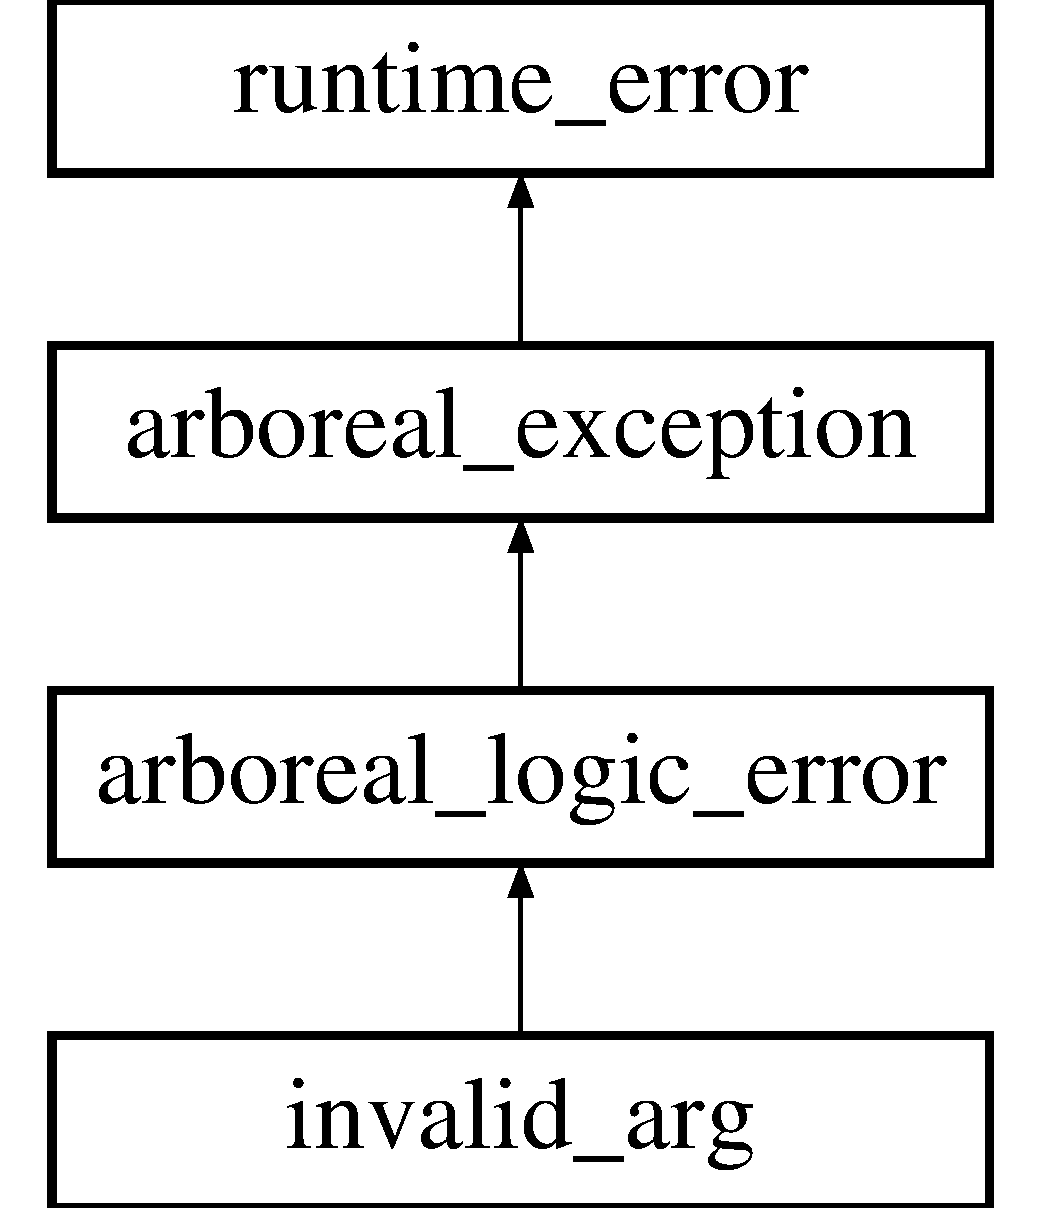
\includegraphics[height=4.000000cm]{classinvalid__arg}
\end{center}
\end{figure}
\subsection*{Public Member Functions}
\begin{DoxyCompactItemize}
\item 
{\bfseries invalid\+\_\+arg} (const char $\ast$what, const char $\ast$where, const int ecode=99)\hypertarget{classinvalid__arg_ab470c1e208290687c57ddb80ad7c91bf}{}\label{classinvalid__arg_ab470c1e208290687c57ddb80ad7c91bf}

\item 
{\bfseries invalid\+\_\+arg} (const char $\ast$what, const string \&where, const int ecode=99)\hypertarget{classinvalid__arg_ac64346933956c640dc48166d3c11ea6d}{}\label{classinvalid__arg_ac64346933956c640dc48166d3c11ea6d}

\item 
{\bfseries invalid\+\_\+arg} (const string \&what, const string \&where, const int ecode=99)\hypertarget{classinvalid__arg_afd1c07ada97de63dd8b2bf8d19753649}{}\label{classinvalid__arg_afd1c07ada97de63dd8b2bf8d19753649}

\item 
{\bfseries invalid\+\_\+arg} (const string \&what, const char $\ast$where, const int ecode=99)\hypertarget{classinvalid__arg_a1b68c46a8c2ddc202eb89edf05667618}{}\label{classinvalid__arg_a1b68c46a8c2ddc202eb89edf05667618}

\end{DoxyCompactItemize}
\subsection*{Additional Inherited Members}


The documentation for this class was generated from the following files\+:\begin{DoxyCompactItemize}
\item 
Shared\+Headers/Arboreal\+\_\+\+Exceptions.\+h\item 
Shared\+C\+P\+P\+Files/Arboreal\+\_\+\+Exceptions.\+cpp\end{DoxyCompactItemize}

\hypertarget{class_modification}{}\section{Modification Class Reference}
\label{class_modification}\index{Modification@{Modification}}


{\ttfamily \#include $<$Trees.\+h$>$}

Inheritance diagram for Modification\+:\begin{figure}[H]
\begin{center}
\leavevmode
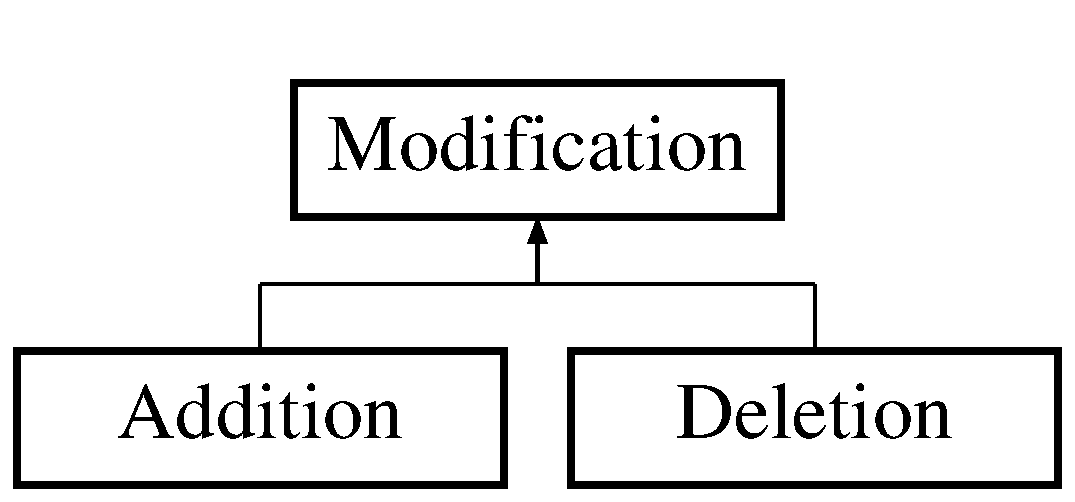
\includegraphics[height=2.000000cm]{class_modification}
\end{center}
\end{figure}
\subsection*{Public Member Functions}
\begin{DoxyCompactItemize}
\item 
virtual \mbox{\hyperlink{class_modification_ab7f5ab083c3be2a3a26f40067b5d22dc}{$\sim$\+Modification}} ()
\item 
virtual void \mbox{\hyperlink{class_modification_a50d1fd809524902d2a1e78d02f4be1dc}{write\+\_\+out}} (\mbox{\hyperlink{class_partition_manager}{Partition\+Manager}} $\ast$pm)=0
\end{DoxyCompactItemize}
\subsection*{Protected Member Functions}
\begin{DoxyCompactItemize}
\item 
\mbox{\hyperlink{class_modification_a76407b8c6d2adb840dceea708355aba8}{Modification}} (\mbox{\hyperlink{class_tree_object}{Tree\+Object}} $\ast$obj, \mbox{\hyperlink{class_tree_object}{Tree\+Object}} $\ast$parent)
\end{DoxyCompactItemize}
\subsection*{Protected Attributes}
\begin{DoxyCompactItemize}
\item 
\mbox{\hyperlink{class_tree_object}{Tree\+Object}} $\ast$ \mbox{\hyperlink{class_modification_a0aa2f9924cde904b1683f3bd80d87a02}{\+\_\+mod}}
\item 
\mbox{\hyperlink{class_tree_object}{Tree\+Object}} $\ast$ \mbox{\hyperlink{class_modification_a529d02be9866b96746bcae63a763f868}{\+\_\+parent}}
\end{DoxyCompactItemize}


\subsection{Constructor \& Destructor Documentation}
\mbox{\Hypertarget{class_modification_a76407b8c6d2adb840dceea708355aba8}\label{class_modification_a76407b8c6d2adb840dceea708355aba8}} 
\index{Modification@{Modification}!Modification@{Modification}}
\index{Modification@{Modification}!Modification@{Modification}}
\subsubsection{\texorpdfstring{Modification()}{Modification()}}
{\footnotesize\ttfamily Modification\+::\+Modification (\begin{DoxyParamCaption}\item[{\mbox{\hyperlink{class_tree_object}{Tree\+Object}} $\ast$}]{obj,  }\item[{\mbox{\hyperlink{class_tree_object}{Tree\+Object}} $\ast$}]{parent }\end{DoxyParamCaption})\hspace{0.3cm}{\ttfamily [protected]}}

\mbox{\Hypertarget{class_modification_ab7f5ab083c3be2a3a26f40067b5d22dc}\label{class_modification_ab7f5ab083c3be2a3a26f40067b5d22dc}} 
\index{Modification@{Modification}!````~Modification@{$\sim$\+Modification}}
\index{````~Modification@{$\sim$\+Modification}!Modification@{Modification}}
\subsubsection{\texorpdfstring{$\sim$\+Modification()}{~Modification()}}
{\footnotesize\ttfamily Modification\+::$\sim$\+Modification (\begin{DoxyParamCaption}{ }\end{DoxyParamCaption})\hspace{0.3cm}{\ttfamily [virtual]}}



\subsection{Member Function Documentation}
\mbox{\Hypertarget{class_modification_a50d1fd809524902d2a1e78d02f4be1dc}\label{class_modification_a50d1fd809524902d2a1e78d02f4be1dc}} 
\index{Modification@{Modification}!write\+\_\+out@{write\+\_\+out}}
\index{write\+\_\+out@{write\+\_\+out}!Modification@{Modification}}
\subsubsection{\texorpdfstring{write\+\_\+out()}{write\_out()}}
{\footnotesize\ttfamily virtual void Modification\+::write\+\_\+out (\begin{DoxyParamCaption}\item[{\mbox{\hyperlink{class_partition_manager}{Partition\+Manager}} $\ast$}]{pm }\end{DoxyParamCaption})\hspace{0.3cm}{\ttfamily [pure virtual]}}



Implemented in \mbox{\hyperlink{class_deletion_ac5bdb21c4a8dbc8afea9910435e509a8}{Deletion}}, and \mbox{\hyperlink{class_addition_a08cd2dae96a62c80d6fe62339232fbca}{Addition}}.



\subsection{Member Data Documentation}
\mbox{\Hypertarget{class_modification_a0aa2f9924cde904b1683f3bd80d87a02}\label{class_modification_a0aa2f9924cde904b1683f3bd80d87a02}} 
\index{Modification@{Modification}!\+\_\+mod@{\+\_\+mod}}
\index{\+\_\+mod@{\+\_\+mod}!Modification@{Modification}}
\subsubsection{\texorpdfstring{\+\_\+mod}{\_mod}}
{\footnotesize\ttfamily \mbox{\hyperlink{class_tree_object}{Tree\+Object}}$\ast$ Modification\+::\+\_\+mod\hspace{0.3cm}{\ttfamily [protected]}}

\mbox{\Hypertarget{class_modification_a529d02be9866b96746bcae63a763f868}\label{class_modification_a529d02be9866b96746bcae63a763f868}} 
\index{Modification@{Modification}!\+\_\+parent@{\+\_\+parent}}
\index{\+\_\+parent@{\+\_\+parent}!Modification@{Modification}}
\subsubsection{\texorpdfstring{\+\_\+parent}{\_parent}}
{\footnotesize\ttfamily \mbox{\hyperlink{class_tree_object}{Tree\+Object}}$\ast$ Modification\+::\+\_\+parent\hspace{0.3cm}{\ttfamily [protected]}}



The documentation for this class was generated from the following files\+:\begin{DoxyCompactItemize}
\item 
Filesystem/\+Daemon\+Dependancies/\+Trees/\mbox{\hyperlink{_trees_8h}{Trees.\+h}}\item 
Filesystem/\+Daemon\+Dependancies/\+Trees/\mbox{\hyperlink{_trees_8cpp}{Trees.\+cpp}}\end{DoxyCompactItemize}

\hypertarget{class_parse_error}{}\section{Parse\+Error Class Reference}
\label{class_parse_error}\index{Parse\+Error@{Parse\+Error}}


{\ttfamily \#include $<$Parser.\+h$>$}

\subsection*{Public Member Functions}
\begin{DoxyCompactItemize}
\item 
\mbox{\hyperlink{class_parse_error_a89210010aa80b9602ef5e57649886937}{Parse\+Error}} (const char $\ast$\mbox{\hyperlink{class_parse_error_aa725d47c84792c9142267e51c2074f58}{where}}, const char $\ast$\mbox{\hyperlink{class_parse_error_a08560dce27779ffee6c4bfb0d796aa6e}{what}})
\end{DoxyCompactItemize}
\begin{Indent}\textbf{ Accessor Functions}\par
\begin{DoxyCompactItemize}
\item 
std\+::string \mbox{\hyperlink{class_parse_error_aa725d47c84792c9142267e51c2074f58}{where}} ()
\item 
std\+::string \mbox{\hyperlink{class_parse_error_a08560dce27779ffee6c4bfb0d796aa6e}{what}} ()
\end{DoxyCompactItemize}
\end{Indent}
\subsection*{Private Attributes}
\begin{DoxyCompactItemize}
\item 
std\+::string \mbox{\hyperlink{class_parse_error_a3a27d02d5a9f461858cefd653a2c4598}{\+\_\+where}}
\item 
std\+::string \mbox{\hyperlink{class_parse_error_a72a23d010120721cde37f0e3203ef12b}{\+\_\+what}}
\end{DoxyCompactItemize}


\subsection{Constructor \& Destructor Documentation}
\mbox{\Hypertarget{class_parse_error_a89210010aa80b9602ef5e57649886937}\label{class_parse_error_a89210010aa80b9602ef5e57649886937}} 
\index{Parse\+Error@{Parse\+Error}!Parse\+Error@{Parse\+Error}}
\index{Parse\+Error@{Parse\+Error}!Parse\+Error@{Parse\+Error}}
\subsubsection{\texorpdfstring{Parse\+Error()}{ParseError()}}
{\footnotesize\ttfamily Parse\+Error\+::\+Parse\+Error (\begin{DoxyParamCaption}\item[{const char $\ast$}]{where,  }\item[{const char $\ast$}]{what }\end{DoxyParamCaption})\hspace{0.3cm}{\ttfamily [inline]}}


\begin{DoxyParams}{Parameters}
{\em where} & Where the parse error took place\\
\hline
{\em what} & What the parse error consisted of \\
\hline
\end{DoxyParams}


\subsection{Member Function Documentation}
\mbox{\Hypertarget{class_parse_error_a08560dce27779ffee6c4bfb0d796aa6e}\label{class_parse_error_a08560dce27779ffee6c4bfb0d796aa6e}} 
\index{Parse\+Error@{Parse\+Error}!what@{what}}
\index{what@{what}!Parse\+Error@{Parse\+Error}}
\subsubsection{\texorpdfstring{what()}{what()}}
{\footnotesize\ttfamily std\+::string Parse\+Error\+::what (\begin{DoxyParamCaption}{ }\end{DoxyParamCaption})\hspace{0.3cm}{\ttfamily [inline]}}

\begin{DoxyReturn}{Returns}
A std\+::string detailing what the parse error consisted of 
\end{DoxyReturn}
\mbox{\Hypertarget{class_parse_error_aa725d47c84792c9142267e51c2074f58}\label{class_parse_error_aa725d47c84792c9142267e51c2074f58}} 
\index{Parse\+Error@{Parse\+Error}!where@{where}}
\index{where@{where}!Parse\+Error@{Parse\+Error}}
\subsubsection{\texorpdfstring{where()}{where()}}
{\footnotesize\ttfamily std\+::string Parse\+Error\+::where (\begin{DoxyParamCaption}{ }\end{DoxyParamCaption})\hspace{0.3cm}{\ttfamily [inline]}}

\begin{DoxyReturn}{Returns}
A std\+::string detailing where the parse error occured 
\end{DoxyReturn}


\subsection{Member Data Documentation}
\mbox{\Hypertarget{class_parse_error_a72a23d010120721cde37f0e3203ef12b}\label{class_parse_error_a72a23d010120721cde37f0e3203ef12b}} 
\index{Parse\+Error@{Parse\+Error}!\+\_\+what@{\+\_\+what}}
\index{\+\_\+what@{\+\_\+what}!Parse\+Error@{Parse\+Error}}
\subsubsection{\texorpdfstring{\+\_\+what}{\_what}}
{\footnotesize\ttfamily std\+::string Parse\+Error\+::\+\_\+what\hspace{0.3cm}{\ttfamily [private]}}

\mbox{\Hypertarget{class_parse_error_a3a27d02d5a9f461858cefd653a2c4598}\label{class_parse_error_a3a27d02d5a9f461858cefd653a2c4598}} 
\index{Parse\+Error@{Parse\+Error}!\+\_\+where@{\+\_\+where}}
\index{\+\_\+where@{\+\_\+where}!Parse\+Error@{Parse\+Error}}
\subsubsection{\texorpdfstring{\+\_\+where}{\_where}}
{\footnotesize\ttfamily std\+::string Parse\+Error\+::\+\_\+where\hspace{0.3cm}{\ttfamily [private]}}



The documentation for this class was generated from the following file\+:\begin{DoxyCompactItemize}
\item 
Shared\+Headers/\mbox{\hyperlink{_parser_8h}{Parser.\+h}}\end{DoxyCompactItemize}

\hypertarget{class_parser}{}\section{Parser Class Reference}
\label{class_parser}\index{Parser@{Parser}}


{\ttfamily \#include $<$Parser.\+h$>$}

\subsection*{Public Member Functions}
\begin{DoxyCompactItemize}
\item 
\mbox{\hyperlink{class_parser_a3e658b5917a93a3ef648050d060e3a93}{$\sim$\+Parser}} ()
\end{DoxyCompactItemize}
\textbf{ }\par
\begin{DoxyCompactItemize}
\item 
\mbox{\hyperlink{class_parser_a306c6c33d7a6cf1bb682be360fcfe982}{Parser}} (char $\ast$buffer, char $\ast$cwd, int max\+\_\+name\+\_\+size)
\item 
\mbox{\hyperlink{class_parser_ada33680bf5f723ef95c44eeed1bff451}{Parser}} (std\+::string string, std\+::string cwd, int max\+\_\+name\+\_\+size)
\item 
\mbox{\hyperlink{class_parser_a5168f5c44e9649e71796f9bef48bdbbe}{Parser}} (const char $\ast$string\+\_\+lit, const char $\ast$cwd, int max\+\_\+name\+\_\+size)
\item 
\mbox{\hyperlink{class_parser_a12234f6cd36b61af4b50c94a179422c1}{Parser}} ()
\end{DoxyCompactItemize}

\begin{Indent}\textbf{ Public Mutators}\par
\begin{DoxyCompactItemize}
\item 
void \mbox{\hyperlink{class_parser_a87f5e73ca10ef5f84f37a4b37e0e6f59}{reset}} (std\+::string string, std\+::string cwd=\char`\"{}\char`\"{})
\begin{DoxyCompactList}\small\item\em Changes the member \+\_\+string of the parser class to whatever is passed. \end{DoxyCompactList}\item 
void \mbox{\hyperlink{class_parser_a5e097c301e171481e8d2af91c112e35e}{reset}} (char $\ast$buffer, char $\ast$cwd=N\+U\+LL)
\begin{DoxyCompactList}\small\item\em Changes the member \+\_\+string of the parser class to whatever is passed. \end{DoxyCompactList}\item 
void \mbox{\hyperlink{class_parser_ab51b81b1617f1948205d73804e3c0fb9}{reset}} (const char $\ast$string\+\_\+lit, const char $\ast$cwd=\char`\"{}\char`\"{})
\begin{DoxyCompactList}\small\item\em Changes the member \+\_\+string of the parser class to whatever is passed. \end{DoxyCompactList}\item 
void \mbox{\hyperlink{class_parser_ac9c3bf43a7f27f92ecf538b83c5984d6}{set\+\_\+max\+\_\+name\+\_\+size}} (int size)
\begin{DoxyCompactList}\small\item\em Sets the maximum allowed file and tagname size that the \mbox{\hyperlink{class_parser}{Parser}} will use. \end{DoxyCompactList}\item 
void \mbox{\hyperlink{class_parser_a086f1431a0cac193fb6ff4506ba5c701}{set\+\_\+cwd}} (std\+::string cwd)
\begin{DoxyCompactList}\small\item\em Sets the Current Working Directory that the \mbox{\hyperlink{class_parser}{Parser}} will use. \end{DoxyCompactList}\end{DoxyCompactItemize}
\end{Indent}
\subsection*{Private Member Functions}
\begin{Indent}\textbf{ Private Helper Functions}\par
\begin{DoxyCompactItemize}
\item 
std\+::vector$<$ std\+::string $>$ \mbox{\hyperlink{class_parser_ac786ab202a25c76a069e124d1bdaa780}{lunion}} (std\+::string string)
\item 
std\+::vector$<$ std\+::string $>$ \mbox{\hyperlink{class_parser_af09e013dcba70865bdff465a7dafba6a}{lintersect}} (std\+::string string)
\item 
std\+::vector$<$ std\+::string $>$ \mbox{\hyperlink{class_parser_ac5276b177af3258fdd2437134652f9df}{matrix\+\_\+multiply}} (std\+::vector$<$ std\+::string $>$ v1, std\+::vector$<$ std\+::string $>$ v2)
\begin{DoxyCompactList}\small\item\em Helper function which performs matrix multiplication on two std\+::vector\textquotesingle{}s of std\+::string\textquotesingle{}s Always multiplies the larger vector into the smaller vector unless the vectors are of equal size. \end{DoxyCompactList}\item 
void \mbox{\hyperlink{class_parser_a8e7cd45cdf0fe9f3420f26a54a946f56}{parse\+\_\+path}} (std\+::vector$<$ std\+::string $>$ \&parsed)
\begin{DoxyCompactList}\small\item\em Removes unnescesarry information (such as the command flags), from a command string which is contains a \char`\"{}path\char`\"{}. \end{DoxyCompactList}\item 
void \mbox{\hyperlink{class_parser_a6e7db54feacd1bff189de70135cd3216}{parse\+\_\+rename}} (std\+::vector$<$ std\+::string $>$ \&parsed)
\begin{DoxyCompactList}\small\item\em Handles the parsing of \textquotesingle{}rename tag\textquotesingle{} commands. \end{DoxyCompactList}\item 
void \mbox{\hyperlink{class_parser_a4dff2c17612843df95b4ec6d4e4af847}{parse\+\_\+merge}} (std\+::vector$<$ std\+::string $>$ \&parsed)
\begin{DoxyCompactList}\small\item\em Handles the parsing of \textquotesingle{}merge tag\textquotesingle{} commands. \end{DoxyCompactList}\item 
void \mbox{\hyperlink{class_parser_abc03a0e1dbb6886981f024cb3957b09a}{jump\+\_\+to\+\_\+char}} (int \&index, char delim)
\begin{DoxyCompactList}\small\item\em Set index to the first instance of the requested char within a std\+::string. \end{DoxyCompactList}\item 
void \mbox{\hyperlink{class_parser_a69c2ea3723b454b2627ecaf0fe7c88ea}{substr\+\_\+to\+\_\+char}} (int \&index, std\+::string \&string, char delim)
\begin{DoxyCompactList}\small\item\em Generates a std\+::string from a given index up until a chosen delimiting charachter Using another std\+::string as its base. \end{DoxyCompactList}\end{DoxyCompactItemize}
\end{Indent}
\subsection*{Private Attributes}
\begin{DoxyCompactItemize}
\item 
std\+::string \mbox{\hyperlink{class_parser_a172a2dcda0488c937d690755d9f4318c}{\+\_\+string}}
\item 
std\+::string \mbox{\hyperlink{class_parser_a3439fb839047252a9c701532ab5f15a0}{\+\_\+cwd}}
\item 
int \mbox{\hyperlink{class_parser_a77c955ec95d7c70515acae6d2e6ad88b}{\+\_\+max\+\_\+name\+\_\+size}}
\end{DoxyCompactItemize}
\subsection*{Public Accessors}
\begin{DoxyCompactItemize}
\item 
std\+::vector$<$ std\+::string $>$ \mbox{\hyperlink{class_parser_a5b531e9ed867eeb8ccb9cb088cf35c24}{parse}} (int type)
\begin{DoxyCompactList}\small\item\em Parse a string based on a certain rule. \end{DoxyCompactList}\item 
std\+::vector$<$ std\+::string $>$ \mbox{\hyperlink{class_parser_aa973764b863dfbe448fa2fd7aa9ffdaa}{get\+\_\+cwd\+\_\+tags}} ()
\begin{DoxyCompactList}\small\item\em Returns a vector representation of the current working directory. \end{DoxyCompactList}\item 
static std\+::vector$<$ std\+::string $>$ \mbox{\hyperlink{class_parser_a71c87961db9707dc18db00a645d3d1e5}{split\+\_\+on\+\_\+delim}} (std\+::string string, char delim)
\begin{DoxyCompactList}\small\item\em Splits a string at each instance of a particualar char (the delimeter) \end{DoxyCompactList}\end{DoxyCompactItemize}


\subsection{Constructor \& Destructor Documentation}
\mbox{\Hypertarget{class_parser_a306c6c33d7a6cf1bb682be360fcfe982}\label{class_parser_a306c6c33d7a6cf1bb682be360fcfe982}} 
\index{Parser@{Parser}!Parser@{Parser}}
\index{Parser@{Parser}!Parser@{Parser}}
\subsubsection{\texorpdfstring{Parser()}{Parser()}\hspace{0.1cm}{\footnotesize\ttfamily [1/4]}}
{\footnotesize\ttfamily Parser\+::\+Parser (\begin{DoxyParamCaption}\item[{char $\ast$}]{buffer,  }\item[{char $\ast$}]{cwd,  }\item[{int}]{max\+\_\+name\+\_\+size }\end{DoxyParamCaption})}

name Constructors;


\begin{DoxyParams}{Parameters}
{\em buffer} & A C-\/\+Style String representation of the string to be parsed\\
\hline
{\em cwd} & A C-\/\+Style String representation of the current working directory; (This value is typically provided by the Liaison process). The directory string is used to parse commands which act within directories only thus providing commands such as \textquotesingle{}tag\textquotesingle{} a \char`\"{}path\char`\"{} to the file(s) which will be tagged without the user having to explicitly enter those file\textquotesingle{}s entire paths themselves.\\
\hline
{\em max\+\_\+name\+\_\+size} & The maximum length that a file or tagname is allowed to have; (This value is typically provided by the Liaison process) \\
\hline
\end{DoxyParams}
\mbox{\Hypertarget{class_parser_ada33680bf5f723ef95c44eeed1bff451}\label{class_parser_ada33680bf5f723ef95c44eeed1bff451}} 
\index{Parser@{Parser}!Parser@{Parser}}
\index{Parser@{Parser}!Parser@{Parser}}
\subsubsection{\texorpdfstring{Parser()}{Parser()}\hspace{0.1cm}{\footnotesize\ttfamily [2/4]}}
{\footnotesize\ttfamily Parser\+::\+Parser (\begin{DoxyParamCaption}\item[{std\+::string}]{string,  }\item[{std\+::string}]{cwd,  }\item[{int}]{max\+\_\+name\+\_\+size }\end{DoxyParamCaption})}


\begin{DoxyParams}{Parameters}
{\em buffer} & A std\+::string representation of the string to be parsed\\
\hline
{\em cwd} & A std\+::string representation of the current working directory; (This value is typically provided by the Liaison process). The directory string is used to parse commands which act within directories only thus, providing commands such as \textquotesingle{}tag\textquotesingle{} a \char`\"{}path\char`\"{} to the file(s) which will be tagged without the user having to explicitly enter those file\textquotesingle{}s entire paths themselves.\\
\hline
{\em max\+\_\+name\+\_\+size} & The maximum length that a file or tagname is allowed to have; (This value is typically provided by the Liaison process) \\
\hline
\end{DoxyParams}
\mbox{\Hypertarget{class_parser_a5168f5c44e9649e71796f9bef48bdbbe}\label{class_parser_a5168f5c44e9649e71796f9bef48bdbbe}} 
\index{Parser@{Parser}!Parser@{Parser}}
\index{Parser@{Parser}!Parser@{Parser}}
\subsubsection{\texorpdfstring{Parser()}{Parser()}\hspace{0.1cm}{\footnotesize\ttfamily [3/4]}}
{\footnotesize\ttfamily Parser\+::\+Parser (\begin{DoxyParamCaption}\item[{const char $\ast$}]{string\+\_\+lit,  }\item[{const char $\ast$}]{cwd,  }\item[{int}]{max\+\_\+name\+\_\+size }\end{DoxyParamCaption})}


\begin{DoxyParams}{Parameters}
{\em buffer} & A String Literal representation of the string to be parsed\\
\hline
{\em cwd} & A String Literal representation of the current working directory; (This value is typically provided by the Liaison process). The directory string is used to parse commands which act within directories only thus, providing commands such as \textquotesingle{}tag\textquotesingle{} a \char`\"{}path\char`\"{} to the file(s) which will be tagged without the user having to explicitly enter those file\textquotesingle{}s entire paths themselves.\\
\hline
{\em max\+\_\+name\+\_\+size} & The maximum length that a file or tagname is allowed to have; (This value is typically provided by the Liaison process) \\
\hline
\end{DoxyParams}
\mbox{\Hypertarget{class_parser_a12234f6cd36b61af4b50c94a179422c1}\label{class_parser_a12234f6cd36b61af4b50c94a179422c1}} 
\index{Parser@{Parser}!Parser@{Parser}}
\index{Parser@{Parser}!Parser@{Parser}}
\subsubsection{\texorpdfstring{Parser()}{Parser()}\hspace{0.1cm}{\footnotesize\ttfamily [4/4]}}
{\footnotesize\ttfamily Parser\+::\+Parser (\begin{DoxyParamCaption}{ }\end{DoxyParamCaption})}

Default Constructor to be used in case initialization of values needs to be done elsewhere \mbox{\Hypertarget{class_parser_a3e658b5917a93a3ef648050d060e3a93}\label{class_parser_a3e658b5917a93a3ef648050d060e3a93}} 
\index{Parser@{Parser}!````~Parser@{$\sim$\+Parser}}
\index{````~Parser@{$\sim$\+Parser}!Parser@{Parser}}
\subsubsection{\texorpdfstring{$\sim$\+Parser()}{~Parser()}}
{\footnotesize\ttfamily Parser\+::$\sim$\+Parser (\begin{DoxyParamCaption}{ }\end{DoxyParamCaption})}

Default Destructor; Does nothing 

\subsection{Member Function Documentation}
\mbox{\Hypertarget{class_parser_aa973764b863dfbe448fa2fd7aa9ffdaa}\label{class_parser_aa973764b863dfbe448fa2fd7aa9ffdaa}} 
\index{Parser@{Parser}!get\+\_\+cwd\+\_\+tags@{get\+\_\+cwd\+\_\+tags}}
\index{get\+\_\+cwd\+\_\+tags@{get\+\_\+cwd\+\_\+tags}!Parser@{Parser}}
\subsubsection{\texorpdfstring{get\+\_\+cwd\+\_\+tags()}{get\_cwd\_tags()}}
{\footnotesize\ttfamily std\+::vector$<$ std\+::string $>$ Parser\+::get\+\_\+cwd\+\_\+tags (\begin{DoxyParamCaption}{ }\end{DoxyParamCaption})}



Returns a vector representation of the current working directory. 

That is, it will decompose \textquotesingle{}/string1/string2\textquotesingle{} into a vector containing \mbox{[}string1, string2\mbox{]}. This is useful when the calling code requires the current working directory as a vector of strings rather than as a standard string representation.

\begin{DoxyReturn}{Returns}
A std\+::vector of std\+::string comprised of the non-\/\textquotesingle{}/\textquotesingle{} parts of the \mbox{\hyperlink{class_parser}{Parser}} member value \+\_\+cwd 
\end{DoxyReturn}
\mbox{\Hypertarget{class_parser_abc03a0e1dbb6886981f024cb3957b09a}\label{class_parser_abc03a0e1dbb6886981f024cb3957b09a}} 
\index{Parser@{Parser}!jump\+\_\+to\+\_\+char@{jump\+\_\+to\+\_\+char}}
\index{jump\+\_\+to\+\_\+char@{jump\+\_\+to\+\_\+char}!Parser@{Parser}}
\subsubsection{\texorpdfstring{jump\+\_\+to\+\_\+char()}{jump\_to\_char()}}
{\footnotesize\ttfamily void Parser\+::jump\+\_\+to\+\_\+char (\begin{DoxyParamCaption}\item[{int \&}]{index,  }\item[{char}]{delim }\end{DoxyParamCaption})\hspace{0.3cm}{\ttfamily [private]}}



Set index to the first instance of the requested char within a std\+::string. 

Because fast forwarding to a specific index (for example in order to skip command flags or other unimportant data (to the parser anyway)) is such a common need, this function was made in order to reduce code duplication. It use the member \+\_\+string as the std\+::string it operates on and will return the index within the std\+::string at which the chose delimeter occurs. It D\+O\+ES N\+OT modify the underling string in any way.


\begin{DoxyParams}{Parameters}
{\em index} & A reference to a variable that will be incremented as the function operates\\
\hline
{\em delim} & A char value which will function as the delimeter at which the function will stop\\
\hline
\end{DoxyParams}
\begin{DoxyReturn}{Returns}
Void 
\end{DoxyReturn}
\mbox{\Hypertarget{class_parser_af09e013dcba70865bdff465a7dafba6a}\label{class_parser_af09e013dcba70865bdff465a7dafba6a}} 
\index{Parser@{Parser}!lintersect@{lintersect}}
\index{lintersect@{lintersect}!Parser@{Parser}}
\subsubsection{\texorpdfstring{lintersect()}{lintersect()}}
{\footnotesize\ttfamily std\+::vector$<$ std\+::string $>$ Parser\+::lintersect (\begin{DoxyParamCaption}\item[{std\+::string}]{string }\end{DoxyParamCaption})\hspace{0.3cm}{\ttfamily [private]}}

Helper function to recursively decompose commands of the form \textquotesingle{}command \{s1,s2,..\}\textquotesingle{}. Is also instrumental in the parsing of \textquotesingle{}find\textquotesingle{} commands in instances were the find command includes list notation (e.\+g. \textquotesingle{}find \{s1,\mbox{[}s2,s3\mbox{]},...\}\textquotesingle{}).


\begin{DoxyParams}{Parameters}
{\em string} & A std\+::string representation of the string which will be decomposed\\
\hline
\end{DoxyParams}
\begin{DoxyReturn}{Returns}
A std\+::vector of std\+::string representing the decomposed string 
\end{DoxyReturn}
\mbox{\Hypertarget{class_parser_ac786ab202a25c76a069e124d1bdaa780}\label{class_parser_ac786ab202a25c76a069e124d1bdaa780}} 
\index{Parser@{Parser}!lunion@{lunion}}
\index{lunion@{lunion}!Parser@{Parser}}
\subsubsection{\texorpdfstring{lunion()}{lunion()}}
{\footnotesize\ttfamily std\+::vector$<$ std\+::string $>$ Parser\+::lunion (\begin{DoxyParamCaption}\item[{std\+::string}]{string }\end{DoxyParamCaption})\hspace{0.3cm}{\ttfamily [private]}}

Helper function to recursively decompose commands of the form \textquotesingle{}command \mbox{[}s1,s2,..\mbox{]}\textquotesingle{}. Is also instrumental in the parsing of \textquotesingle{}find\textquotesingle{} commands in instances were the find command includes set notation (e.\+g. \textquotesingle{}find \mbox{[}s1,\{s2,s3\},...\mbox{]}\textquotesingle{}).


\begin{DoxyParams}{Parameters}
{\em string} & A std\+::string representation of the string which will be decomposed\\
\hline
\end{DoxyParams}
\begin{DoxyReturn}{Returns}
A std\+::vector of std\+::string representing the decomposed string 
\end{DoxyReturn}
\mbox{\Hypertarget{class_parser_ac5276b177af3258fdd2437134652f9df}\label{class_parser_ac5276b177af3258fdd2437134652f9df}} 
\index{Parser@{Parser}!matrix\+\_\+multiply@{matrix\+\_\+multiply}}
\index{matrix\+\_\+multiply@{matrix\+\_\+multiply}!Parser@{Parser}}
\subsubsection{\texorpdfstring{matrix\+\_\+multiply()}{matrix\_multiply()}}
{\footnotesize\ttfamily std\+::vector$<$ std\+::string $>$ Parser\+::matrix\+\_\+multiply (\begin{DoxyParamCaption}\item[{std\+::vector$<$ std\+::string $>$}]{v1,  }\item[{std\+::vector$<$ std\+::string $>$}]{v2 }\end{DoxyParamCaption})\hspace{0.3cm}{\ttfamily [private]}}



Helper function which performs matrix multiplication on two std\+::vector\textquotesingle{}s of std\+::string\textquotesingle{}s Always multiplies the larger vector into the smaller vector unless the vectors are of equal size. 

Used to create strings for \textquotesingle{}find\textquotesingle{} commands which are of the form \textquotesingle{}\{s1,\mbox{[}s2,s3\mbox{]},...\}\textquotesingle{}. The \textquotesingle{}\{\}\textquotesingle{} construction is an \&\& construction, that is, it finds all files tagged with A\+LL of the strings within the braces. However, the \textquotesingle{}\mbox{[}\mbox{]}\textquotesingle{} construction is an $\vert$$\vert$ construction and finds all files tagged with A\+NY of the strings vithin the brackets. This means that a construction like \textquotesingle{}\{s1,\mbox{[}s2,s3\mbox{]},s4..\}\textquotesingle{} must find files tagged with\+: \{s1,s2,s4..\}, \{s1,s3,s4..\} the best way to achieve these results is to matrix multiply the vector returned by \mbox{\hyperlink{class_parser_ac786ab202a25c76a069e124d1bdaa780}{lunion()}} (which handles \textquotesingle{}\mbox{[}\mbox{]}\textquotesingle{} constructions) and \mbox{\hyperlink{class_parser_af09e013dcba70865bdff465a7dafba6a}{lintersect()}} (which handles \textquotesingle{}\{\}\textquotesingle{} constructions). Note that this has cubic time comlexity and so should be used sparingly for very large vectors.


\begin{DoxyParams}{Parameters}
{\em v1} & One of the std\+::vector\textquotesingle{}s of std\+::string\textquotesingle{}s that will be multiplied \\
\hline
{\em v2} & The other of the std\+::vector\textquotesingle{}s of std\+::string\textquotesingle{}s that will be multiplied\\
\hline
\end{DoxyParams}
\begin{DoxyReturn}{Returns}
A std\+::vector of std\+::string\textquotesingle{}s representing the matrix multiplication of v1 \& v2 
\end{DoxyReturn}
\mbox{\Hypertarget{class_parser_a5b531e9ed867eeb8ccb9cb088cf35c24}\label{class_parser_a5b531e9ed867eeb8ccb9cb088cf35c24}} 
\index{Parser@{Parser}!parse@{parse}}
\index{parse@{parse}!Parser@{Parser}}
\subsubsection{\texorpdfstring{parse()}{parse()}}
{\footnotesize\ttfamily std\+::vector$<$ std\+::string $>$ Parser\+::parse (\begin{DoxyParamCaption}\item[{int}]{type }\end{DoxyParamCaption})}



Parse a string based on a certain rule. 

The rule generally corresponds to how a C\+LI command should be decomposed. ~\newline
For example the C\+LI command for finding files takes a list of files, hower the C\+LI itself does not support batch commands, therefore, the \mbox{\hyperlink{class_parser}{Parser}} will decompose the command into its constituent parts (i.\+e. a single file). ~\newline
This particular behavior is access by passing \textquotesingle{}8\textquotesingle{} as the \char`\"{}type\char`\"{} of decomposition that needs to take place (Note that this corresponds to the command\textquotesingle{}s ID). ~\newline
However the \mbox{\hyperlink{class_parser}{Parser}} can be extended to support any rule whatsoever, so long as it is added to the \mbox{\hyperlink{class_parser}{Parser}}\textquotesingle{}s \mbox{\hyperlink{class_parser_a5b531e9ed867eeb8ccb9cb088cf35c24}{parse()}} function switch statement.


\begin{DoxyParams}{Parameters}
{\em type} & The integer identification of the parse rule that will be executed\\
\hline
\end{DoxyParams}
\begin{DoxyReturn}{Returns}
A std\+::vector of std\+::string comprised of the result after the chosen parse rule is executed. 
\end{DoxyReturn}
\mbox{\Hypertarget{class_parser_a4dff2c17612843df95b4ec6d4e4af847}\label{class_parser_a4dff2c17612843df95b4ec6d4e4af847}} 
\index{Parser@{Parser}!parse\+\_\+merge@{parse\+\_\+merge}}
\index{parse\+\_\+merge@{parse\+\_\+merge}!Parser@{Parser}}
\subsubsection{\texorpdfstring{parse\+\_\+merge()}{parse\_merge()}}
{\footnotesize\ttfamily void Parser\+::parse\+\_\+merge (\begin{DoxyParamCaption}\item[{std\+::vector$<$ std\+::string $>$ \&}]{parsed }\end{DoxyParamCaption})\hspace{0.3cm}{\ttfamily [private]}}



Handles the parsing of \textquotesingle{}merge tag\textquotesingle{} commands. 

The \textquotesingle{}merge tags\textquotesingle{} commands have syntax that does not conorm well with the rest of the commands Therefore because of their uniqueness and in an effort to reduce \char`\"{}\+Walls of Text\char`\"{} they were separated into their own function. \mbox{\hyperlink{class_parser_a4dff2c17612843df95b4ec6d4e4af847}{parse\+\_\+merge()}} will decompose the command \textquotesingle{}merge \mbox{[}t1,t2,...\mbox{]} =$>$ tx\textquotesingle{} into multiple single merge operations of the form \textquotesingle{}t1-\/tx\textquotesingle{}, \textquotesingle{}t2-\/tx\textquotesingle{}, etc. and add them to the vector that the \mbox{\hyperlink{class_parser}{Parser}} will return upon successful completion of \mbox{\hyperlink{class_parser_a5b531e9ed867eeb8ccb9cb088cf35c24}{parse()}}


\begin{DoxyParams}{Parameters}
{\em parsed} & A referance to the std\+::vector into which the reduced command will be added. In general this should be the std\+::vector that the \mbox{\hyperlink{class_parser}{Parser}} will return upon successful completion of \mbox{\hyperlink{class_parser_a5b531e9ed867eeb8ccb9cb088cf35c24}{parse()}} \\
\hline
\end{DoxyParams}
\mbox{\Hypertarget{class_parser_a8e7cd45cdf0fe9f3420f26a54a946f56}\label{class_parser_a8e7cd45cdf0fe9f3420f26a54a946f56}} 
\index{Parser@{Parser}!parse\+\_\+path@{parse\+\_\+path}}
\index{parse\+\_\+path@{parse\+\_\+path}!Parser@{Parser}}
\subsubsection{\texorpdfstring{parse\+\_\+path()}{parse\_path()}}
{\footnotesize\ttfamily void Parser\+::parse\+\_\+path (\begin{DoxyParamCaption}\item[{std\+::vector$<$ std\+::string $>$ \&}]{parsed }\end{DoxyParamCaption})\hspace{0.3cm}{\ttfamily [private]}}



Removes unnescesarry information (such as the command flags), from a command string which is contains a \char`\"{}path\char`\"{}. 

For example, the command \textquotesingle{}delete /tag1/tag2/file\textquotesingle{} would be reduced to \textquotesingle{}/tag1/tag2/file\textquotesingle{}


\begin{DoxyParams}{Parameters}
{\em parsed} & A referance to the std\+::vector into which the reduced command will be added. In general this should be the std\+::vector that the \mbox{\hyperlink{class_parser}{Parser}} will return upon successful completion of \mbox{\hyperlink{class_parser_a5b531e9ed867eeb8ccb9cb088cf35c24}{parse()}}\\
\hline
\end{DoxyParams}
\begin{DoxyReturn}{Returns}
Void 
\end{DoxyReturn}
\mbox{\Hypertarget{class_parser_a6e7db54feacd1bff189de70135cd3216}\label{class_parser_a6e7db54feacd1bff189de70135cd3216}} 
\index{Parser@{Parser}!parse\+\_\+rename@{parse\+\_\+rename}}
\index{parse\+\_\+rename@{parse\+\_\+rename}!Parser@{Parser}}
\subsubsection{\texorpdfstring{parse\+\_\+rename()}{parse\_rename()}}
{\footnotesize\ttfamily void Parser\+::parse\+\_\+rename (\begin{DoxyParamCaption}\item[{std\+::vector$<$ std\+::string $>$ \&}]{parsed }\end{DoxyParamCaption})\hspace{0.3cm}{\ttfamily [private]}}



Handles the parsing of \textquotesingle{}rename tag\textquotesingle{} commands. 

The \textquotesingle{}rename tag\textquotesingle{} commands must decomposes two seperate lists and then join each value at index = x in either list together. That is, the value at index 1 in list 1 must be joined with the value at index 1 in list 2. parse\+\_\+rname() performs this function and adds the result to the vector that the \mbox{\hyperlink{class_parser}{Parser}} will return upon the successful completion of \mbox{\hyperlink{class_parser_a5b531e9ed867eeb8ccb9cb088cf35c24}{parse()}}, in the following format \textquotesingle{}list1value-\/list2value\textquotesingle{}. In an effort to reduce \char`\"{}\+Walls of Text\char`\"{} and because of the uniqueness of this command, this particular algorithm was placed into its own function.


\begin{DoxyParams}{Parameters}
{\em parsed} & A referance to the std\+::vector into which the reduced command will be added. In general this should be the std\+::vector that the \mbox{\hyperlink{class_parser}{Parser}} will return upon successful completion of \mbox{\hyperlink{class_parser_a5b531e9ed867eeb8ccb9cb088cf35c24}{parse()}}\\
\hline
\end{DoxyParams}
\begin{DoxyReturn}{Returns}
Void 
\end{DoxyReturn}
\mbox{\Hypertarget{class_parser_a87f5e73ca10ef5f84f37a4b37e0e6f59}\label{class_parser_a87f5e73ca10ef5f84f37a4b37e0e6f59}} 
\index{Parser@{Parser}!reset@{reset}}
\index{reset@{reset}!Parser@{Parser}}
\subsubsection{\texorpdfstring{reset()}{reset()}\hspace{0.1cm}{\footnotesize\ttfamily [1/3]}}
{\footnotesize\ttfamily void Parser\+::reset (\begin{DoxyParamCaption}\item[{std\+::string}]{string,  }\item[{std\+::string}]{cwd = {\ttfamily \char`\"{}\char`\"{}} }\end{DoxyParamCaption})}



Changes the member \+\_\+string of the parser class to whatever is passed. 

The \mbox{\hyperlink{class_parser}{Parser}} class conducts all operations on its member \+\_\+string rather than requiring that a string value be passed to its \mbox{\hyperlink{class_parser_a5b531e9ed867eeb8ccb9cb088cf35c24}{parse()}} method. This was done in order to make use of the class as streamlined as possible.


\begin{DoxyParams}{Parameters}
{\em string} & A std\+::string representation of the string to be parsed\\
\hline
{\em cwd} & A std\+::string representation of the current working directory; Note that this argument is optional and allows the user to both reset the string the \mbox{\hyperlink{class_parser}{Parser}} will work with as well as the directory string the \mbox{\hyperlink{class_parser}{Parser}} will use. The directory string is used to parse commands which act within directories only thus providing commands such as \textquotesingle{}tag\textquotesingle{} a \char`\"{}path\char`\"{} to the file(s) which will be tagged without the user having to explicitly enter those file\textquotesingle{}s entire paths themselves. \\
\hline
\end{DoxyParams}
\mbox{\Hypertarget{class_parser_a5e097c301e171481e8d2af91c112e35e}\label{class_parser_a5e097c301e171481e8d2af91c112e35e}} 
\index{Parser@{Parser}!reset@{reset}}
\index{reset@{reset}!Parser@{Parser}}
\subsubsection{\texorpdfstring{reset()}{reset()}\hspace{0.1cm}{\footnotesize\ttfamily [2/3]}}
{\footnotesize\ttfamily void Parser\+::reset (\begin{DoxyParamCaption}\item[{char $\ast$}]{buffer,  }\item[{char $\ast$}]{cwd = {\ttfamily NULL} }\end{DoxyParamCaption})}



Changes the member \+\_\+string of the parser class to whatever is passed. 

The \mbox{\hyperlink{class_parser}{Parser}} class conducts all operations on its member \+\_\+string rather than requiring that a string value be passed to its \mbox{\hyperlink{class_parser_a5b531e9ed867eeb8ccb9cb088cf35c24}{parse()}} method. This was done in order to make use of the class as streamlined as possible.


\begin{DoxyParams}{Parameters}
{\em string} & A C-\/\+Style String representation of the string to be parsed\\
\hline
{\em cwd} & A C-\/\+Style String representation of the current working directory; Note that this argument is optional and allows the user to both reset the string the \mbox{\hyperlink{class_parser}{Parser}} will work with as well as the directory string the \mbox{\hyperlink{class_parser}{Parser}} will use. The directory string is used to parse commands which act within directories only thus providing commands such as \textquotesingle{}tag\textquotesingle{} a \char`\"{}path\char`\"{} to the file(s) which will be tagged without the user having to explicitly enter those file\textquotesingle{}s entire paths themselves.\\
\hline
\end{DoxyParams}
\begin{DoxyReturn}{Returns}
Void 
\end{DoxyReturn}
\mbox{\Hypertarget{class_parser_ab51b81b1617f1948205d73804e3c0fb9}\label{class_parser_ab51b81b1617f1948205d73804e3c0fb9}} 
\index{Parser@{Parser}!reset@{reset}}
\index{reset@{reset}!Parser@{Parser}}
\subsubsection{\texorpdfstring{reset()}{reset()}\hspace{0.1cm}{\footnotesize\ttfamily [3/3]}}
{\footnotesize\ttfamily void Parser\+::reset (\begin{DoxyParamCaption}\item[{const char $\ast$}]{string\+\_\+lit,  }\item[{const char $\ast$}]{cwd = {\ttfamily \char`\"{}\char`\"{}} }\end{DoxyParamCaption})}



Changes the member \+\_\+string of the parser class to whatever is passed. 

The \mbox{\hyperlink{class_parser}{Parser}} class conducts all operations on its member \+\_\+string rather than requiring that a string value be passed to its \mbox{\hyperlink{class_parser_a5b531e9ed867eeb8ccb9cb088cf35c24}{parse()}} method. This was done in order to make use of the class as streamlined as possible.


\begin{DoxyParams}{Parameters}
{\em string} & A String Literal representation of the string to be parsed\\
\hline
{\em cwd} & A String Literal representation of the current working directory; Note that this argument is optional and allows the user to both reset the string the \mbox{\hyperlink{class_parser}{Parser}} will work with as well as the directory string the \mbox{\hyperlink{class_parser}{Parser}} will use. The directory string is used to parse commands which act within directories only thus providing commands such as \textquotesingle{}tag\textquotesingle{} a \char`\"{}path\char`\"{} to the file(s) which will be tagged without the user having to explicitly enter those file\textquotesingle{}s entire paths themselves.\\
\hline
\end{DoxyParams}
\begin{DoxyReturn}{Returns}
Void 
\end{DoxyReturn}
\mbox{\Hypertarget{class_parser_a086f1431a0cac193fb6ff4506ba5c701}\label{class_parser_a086f1431a0cac193fb6ff4506ba5c701}} 
\index{Parser@{Parser}!set\+\_\+cwd@{set\+\_\+cwd}}
\index{set\+\_\+cwd@{set\+\_\+cwd}!Parser@{Parser}}
\subsubsection{\texorpdfstring{set\+\_\+cwd()}{set\_cwd()}}
{\footnotesize\ttfamily void Parser\+::set\+\_\+cwd (\begin{DoxyParamCaption}\item[{std\+::string}]{cwd }\end{DoxyParamCaption})}



Sets the Current Working Directory that the \mbox{\hyperlink{class_parser}{Parser}} will use. 

The directory string is used to parse commands which act within directories only thus providing commands such as \textquotesingle{}tag\textquotesingle{} a \char`\"{}path\char`\"{} to the file(s) which will be tagged without the user having to explicitly enter those file\textquotesingle{}s entire paths themselves. This function does not have counterparts which tahe C-\/\+Style Strings or String Literals. This is because, in all situations, if the current working directory must be set using this method, it is highly likely that the calling code has a std\+::string representation of the current working directory rather than a representation in one of the other formats. If such functionality (C-\/\+Style Strings and others) is desired, extensibility is easy enough. Regardless the \mbox{\hyperlink{class_parser}{Parser}}\textquotesingle{}s \+\_\+cwd member will always be a std\+::string.


\begin{DoxyParams}{Parameters}
{\em cwd} & A std\+::string representation of the current working directory\\
\hline
\end{DoxyParams}
\begin{DoxyReturn}{Returns}
Void 
\end{DoxyReturn}
\mbox{\Hypertarget{class_parser_ac9c3bf43a7f27f92ecf538b83c5984d6}\label{class_parser_ac9c3bf43a7f27f92ecf538b83c5984d6}} 
\index{Parser@{Parser}!set\+\_\+max\+\_\+name\+\_\+size@{set\+\_\+max\+\_\+name\+\_\+size}}
\index{set\+\_\+max\+\_\+name\+\_\+size@{set\+\_\+max\+\_\+name\+\_\+size}!Parser@{Parser}}
\subsubsection{\texorpdfstring{set\+\_\+max\+\_\+name\+\_\+size()}{set\_max\_name\_size()}}
{\footnotesize\ttfamily void Parser\+::set\+\_\+max\+\_\+name\+\_\+size (\begin{DoxyParamCaption}\item[{int}]{size }\end{DoxyParamCaption})}



Sets the maximum allowed file and tagname size that the \mbox{\hyperlink{class_parser}{Parser}} will use. 

If this size is exceeded an error is thrown and the \mbox{\hyperlink{class_parser}{Parser}} will stop its current activities. This value is dictated by the C\+LI and is generally provided to the \mbox{\hyperlink{class_parser}{Parser}} by the Liaison Process.


\begin{DoxyParams}{Parameters}
{\em size} & The maximum file/tag name length \\
\hline
\end{DoxyParams}
\mbox{\Hypertarget{class_parser_a71c87961db9707dc18db00a645d3d1e5}\label{class_parser_a71c87961db9707dc18db00a645d3d1e5}} 
\index{Parser@{Parser}!split\+\_\+on\+\_\+delim@{split\+\_\+on\+\_\+delim}}
\index{split\+\_\+on\+\_\+delim@{split\+\_\+on\+\_\+delim}!Parser@{Parser}}
\subsubsection{\texorpdfstring{split\+\_\+on\+\_\+delim()}{split\_on\_delim()}}
{\footnotesize\ttfamily std\+::vector$<$ std\+::string $>$ Parser\+::split\+\_\+on\+\_\+delim (\begin{DoxyParamCaption}\item[{std\+::string}]{string,  }\item[{char}]{delim }\end{DoxyParamCaption})\hspace{0.3cm}{\ttfamily [static]}}



Splits a string at each instance of a particualar char (the delimeter) 

The delimeters are N\+OT included anywhere in the resulting vector. This function is static and is mainly used outside the \mbox{\hyperlink{class_parser}{Parser}} in order to split values that the parser returned. This can happen because the complexity of certain commands does not allow the parser to fully decompose the string and instead it can only reorganize the command into a form which can be easily split later. It is important to note that this function does not differentiate between the number of delimeter charcters the string contains. That is, it will read the whole string and split it at any point where the delimeter is seen whether it is seen in 1 or 100 places.


\begin{DoxyParams}{Parameters}
{\em string} & A std\+::string representation of whatever string needs to be split \\
\hline
{\em delim} & A char value representing where the string should be split \\
\hline
\end{DoxyParams}
\mbox{\Hypertarget{class_parser_a69c2ea3723b454b2627ecaf0fe7c88ea}\label{class_parser_a69c2ea3723b454b2627ecaf0fe7c88ea}} 
\index{Parser@{Parser}!substr\+\_\+to\+\_\+char@{substr\+\_\+to\+\_\+char}}
\index{substr\+\_\+to\+\_\+char@{substr\+\_\+to\+\_\+char}!Parser@{Parser}}
\subsubsection{\texorpdfstring{substr\+\_\+to\+\_\+char()}{substr\_to\_char()}}
{\footnotesize\ttfamily void Parser\+::substr\+\_\+to\+\_\+char (\begin{DoxyParamCaption}\item[{int \&}]{index,  }\item[{std\+::string \&}]{string,  }\item[{char}]{delim }\end{DoxyParamCaption})\hspace{0.3cm}{\ttfamily [private]}}



Generates a std\+::string from a given index up until a chosen delimiting charachter Using another std\+::string as its base. 

Because the process of creating substrings from starting at an arbitrary index and ending at a specific charachter is so common, this function was created in order to reduce code duplication. This function will generate a string from a given index up until a chosen delimiting charachter. It also saves the resulting end index. This function D\+O\+ES N\+OT modify the underling std\+::string in any way and like other functions above, uses the member \+\_\+string as its underlying std\+::string.


\begin{DoxyParams}{Parameters}
{\em index} & A reference to a variable that will be incremented as the function operates. This serves as both the starting index and the will store the resulting index after the function completes.\\
\hline
{\em string} & A reference to a std\+::string that will be modified with a subset of the contents of the base string.\\
\hline
{\em delim} & The delimiting charachter which will mark the stopping point of the function\\
\hline
\end{DoxyParams}
\begin{DoxyReturn}{Returns}
Void 
\end{DoxyReturn}


\subsection{Member Data Documentation}
\mbox{\Hypertarget{class_parser_a3439fb839047252a9c701532ab5f15a0}\label{class_parser_a3439fb839047252a9c701532ab5f15a0}} 
\index{Parser@{Parser}!\+\_\+cwd@{\+\_\+cwd}}
\index{\+\_\+cwd@{\+\_\+cwd}!Parser@{Parser}}
\subsubsection{\texorpdfstring{\+\_\+cwd}{\_cwd}}
{\footnotesize\ttfamily std\+::string Parser\+::\+\_\+cwd\hspace{0.3cm}{\ttfamily [private]}}

\mbox{\Hypertarget{class_parser_a77c955ec95d7c70515acae6d2e6ad88b}\label{class_parser_a77c955ec95d7c70515acae6d2e6ad88b}} 
\index{Parser@{Parser}!\+\_\+max\+\_\+name\+\_\+size@{\+\_\+max\+\_\+name\+\_\+size}}
\index{\+\_\+max\+\_\+name\+\_\+size@{\+\_\+max\+\_\+name\+\_\+size}!Parser@{Parser}}
\subsubsection{\texorpdfstring{\+\_\+max\+\_\+name\+\_\+size}{\_max\_name\_size}}
{\footnotesize\ttfamily int Parser\+::\+\_\+max\+\_\+name\+\_\+size\hspace{0.3cm}{\ttfamily [private]}}

\mbox{\Hypertarget{class_parser_a172a2dcda0488c937d690755d9f4318c}\label{class_parser_a172a2dcda0488c937d690755d9f4318c}} 
\index{Parser@{Parser}!\+\_\+string@{\+\_\+string}}
\index{\+\_\+string@{\+\_\+string}!Parser@{Parser}}
\subsubsection{\texorpdfstring{\+\_\+string}{\_string}}
{\footnotesize\ttfamily std\+::string Parser\+::\+\_\+string\hspace{0.3cm}{\ttfamily [private]}}



The documentation for this class was generated from the following files\+:\begin{DoxyCompactItemize}
\item 
Shared\+Headers/\mbox{\hyperlink{_parser_8h}{Parser.\+h}}\item 
Shared\+C\+P\+P\+Files/\mbox{\hyperlink{_parser_8cpp}{Parser.\+cpp}}\end{DoxyCompactItemize}

\hypertarget{class_partition_manager}{}\section{Partition\+Manager Class Reference}
\label{class_partition_manager}\index{Partition\+Manager@{Partition\+Manager}}


{\ttfamily \#include $<$Partition\+Manager.\+h$>$}

\subsection*{Public Member Functions}
\begin{DoxyCompactItemize}
\item 
\mbox{\hyperlink{class_partition_manager_aa875b0b19b7ab9f32b02d2c9be383b75}{Partition\+Manager}} (\mbox{\hyperlink{class_disk_manager}{Disk\+Manager}} $\ast$\mbox{\hyperlink{daemon_8h_aa4c8f283fd621cbde00155b93e826d00}{dm}}, string partition\+Name)
\item 
\mbox{\hyperlink{class_partition_manager_aa8ab74a681e67990ae59054a7b7daafe}{$\sim$\+Partition\+Manager}} ()
\end{DoxyCompactItemize}
\begin{Indent}\textbf{ Accessor Functions}\par
\begin{DoxyCompactItemize}
\item 
void \mbox{\hyperlink{class_partition_manager_a7aca34c24770b7b9290c489475655ada}{read\+Disk\+Block}} (Blk\+Num\+Type blknum, char $\ast$blkdata)
\item 
size\+\_\+t \mbox{\hyperlink{class_partition_manager_aa1026e17e77f154d7034fafd188bda02}{get\+Block\+Size}} ()
\item 
string \mbox{\hyperlink{class_partition_manager_a7c756dba2665e5a7b62b2ccb261f1158}{get\+Partition\+Name}} ()
\item 
int \mbox{\hyperlink{class_partition_manager_a3b047c1c63c2f9a9e04805471c04ccf0}{get\+\_\+file\+\_\+name\+\_\+size}} ()
\end{DoxyCompactItemize}
\end{Indent}
\begin{Indent}\textbf{ Modifier Functions}\par
\begin{DoxyCompactItemize}
\item 
void \mbox{\hyperlink{class_partition_manager_a114d5d4f8d90b6e9207b09d99e246bed}{write\+Disk\+Block}} (Blk\+Num\+Type blknum, char $\ast$blkdata)
\item 
Blk\+Num\+Type \mbox{\hyperlink{class_partition_manager_a682ce5963a31cf7009455cb1c229b26a}{get\+Free\+Disk\+Block}} ()
\item 
void \mbox{\hyperlink{class_partition_manager_a3ce9b50aa5e7d9063919fc55d125246b}{return\+Disk\+Block}} (Blk\+Num\+Type blknum)
\end{DoxyCompactItemize}
\end{Indent}
\subsection*{Private Attributes}
\begin{DoxyCompactItemize}
\item 
string \mbox{\hyperlink{class_partition_manager_abce2f4d0702d84f4fafd604a4d6177bc}{\+\_\+partition\+Name}}
\item 
Blk\+Num\+Type \mbox{\hyperlink{class_partition_manager_adc40203c47c043cbef87bd5299462861}{\+\_\+partition\+Size}}
\item 
Blk\+Num\+Type \mbox{\hyperlink{class_partition_manager_aef90b039f531993d85ecca490e6372c0}{\+\_\+free\+Block\+Start}}
\item 
Blk\+Num\+Type \mbox{\hyperlink{class_partition_manager_a76dddfb3211f1a6bb428ea883c16f9fe}{\+\_\+free\+Block\+End}}
\item 
Blk\+Num\+Type \mbox{\hyperlink{class_partition_manager_aec878e091e469ed20dc49c932ae22ad3}{\+\_\+partition\+Blk\+Start}}
\item 
int \mbox{\hyperlink{class_partition_manager_aa934a144c41a546a83c80965428bc0dd}{\+\_\+file\+Name\+Size}}
\item 
\mbox{\hyperlink{class_disk_manager}{Disk\+Manager}} $\ast$ \mbox{\hyperlink{class_partition_manager_a87f98cf8538d89dd4b2bb46ea33d85cd}{\+\_\+my\+DM}}
\end{DoxyCompactItemize}


\subsection{Constructor \& Destructor Documentation}
\mbox{\Hypertarget{class_partition_manager_aa875b0b19b7ab9f32b02d2c9be383b75}\label{class_partition_manager_aa875b0b19b7ab9f32b02d2c9be383b75}} 
\index{Partition\+Manager@{Partition\+Manager}!Partition\+Manager@{Partition\+Manager}}
\index{Partition\+Manager@{Partition\+Manager}!Partition\+Manager@{Partition\+Manager}}
\subsubsection{\texorpdfstring{Partition\+Manager()}{PartitionManager()}}
{\footnotesize\ttfamily Partition\+Manager\+::\+Partition\+Manager (\begin{DoxyParamCaption}\item[{\mbox{\hyperlink{class_disk_manager}{Disk\+Manager}} $\ast$}]{dm,  }\item[{string}]{partition\+Name }\end{DoxyParamCaption})}


\begin{DoxyParams}{Parameters}
{\em dm} & the \mbox{\hyperlink{class_disk_manager}{Disk\+Manager}} associated with this object \\
\hline
{\em partition\+Name} & the name of the partition that this will be managing \\
\hline
\end{DoxyParams}
\mbox{\Hypertarget{class_partition_manager_aa8ab74a681e67990ae59054a7b7daafe}\label{class_partition_manager_aa8ab74a681e67990ae59054a7b7daafe}} 
\index{Partition\+Manager@{Partition\+Manager}!````~Partition\+Manager@{$\sim$\+Partition\+Manager}}
\index{````~Partition\+Manager@{$\sim$\+Partition\+Manager}!Partition\+Manager@{Partition\+Manager}}
\subsubsection{\texorpdfstring{$\sim$\+Partition\+Manager()}{~PartitionManager()}}
{\footnotesize\ttfamily Partition\+Manager\+::$\sim$\+Partition\+Manager (\begin{DoxyParamCaption}{ }\end{DoxyParamCaption})}



\subsection{Member Function Documentation}
\mbox{\Hypertarget{class_partition_manager_a3b047c1c63c2f9a9e04805471c04ccf0}\label{class_partition_manager_a3b047c1c63c2f9a9e04805471c04ccf0}} 
\index{Partition\+Manager@{Partition\+Manager}!get\+\_\+file\+\_\+name\+\_\+size@{get\+\_\+file\+\_\+name\+\_\+size}}
\index{get\+\_\+file\+\_\+name\+\_\+size@{get\+\_\+file\+\_\+name\+\_\+size}!Partition\+Manager@{Partition\+Manager}}
\subsubsection{\texorpdfstring{get\+\_\+file\+\_\+name\+\_\+size()}{get\_file\_name\_size()}}
{\footnotesize\ttfamily int Partition\+Manager\+::get\+\_\+file\+\_\+name\+\_\+size (\begin{DoxyParamCaption}{ }\end{DoxyParamCaption})}

\begin{DoxyReturn}{Returns}
The maximum file name size for this partition in bytes 
\end{DoxyReturn}
\mbox{\Hypertarget{class_partition_manager_aa1026e17e77f154d7034fafd188bda02}\label{class_partition_manager_aa1026e17e77f154d7034fafd188bda02}} 
\index{Partition\+Manager@{Partition\+Manager}!get\+Block\+Size@{get\+Block\+Size}}
\index{get\+Block\+Size@{get\+Block\+Size}!Partition\+Manager@{Partition\+Manager}}
\subsubsection{\texorpdfstring{get\+Block\+Size()}{getBlockSize()}}
{\footnotesize\ttfamily size\+\_\+t Partition\+Manager\+::get\+Block\+Size (\begin{DoxyParamCaption}{ }\end{DoxyParamCaption})}

\begin{DoxyReturn}{Returns}
the blocksize of the \mbox{\hyperlink{class_disk}{Disk}} 
\end{DoxyReturn}
\mbox{\Hypertarget{class_partition_manager_a682ce5963a31cf7009455cb1c229b26a}\label{class_partition_manager_a682ce5963a31cf7009455cb1c229b26a}} 
\index{Partition\+Manager@{Partition\+Manager}!get\+Free\+Disk\+Block@{get\+Free\+Disk\+Block}}
\index{get\+Free\+Disk\+Block@{get\+Free\+Disk\+Block}!Partition\+Manager@{Partition\+Manager}}
\subsubsection{\texorpdfstring{get\+Free\+Disk\+Block()}{getFreeDiskBlock()}}
{\footnotesize\ttfamily Blk\+Num\+Type Partition\+Manager\+::get\+Free\+Disk\+Block (\begin{DoxyParamCaption}{ }\end{DoxyParamCaption})}

Allocates a block on disk if there is a free one. The \mbox{\hyperlink{class_disk}{Disk}} free list is updated accordingly \begin{DoxyReturn}{Returns}
the block number of the newly allocated block 
\end{DoxyReturn}
\mbox{\Hypertarget{class_partition_manager_a7c756dba2665e5a7b62b2ccb261f1158}\label{class_partition_manager_a7c756dba2665e5a7b62b2ccb261f1158}} 
\index{Partition\+Manager@{Partition\+Manager}!get\+Partition\+Name@{get\+Partition\+Name}}
\index{get\+Partition\+Name@{get\+Partition\+Name}!Partition\+Manager@{Partition\+Manager}}
\subsubsection{\texorpdfstring{get\+Partition\+Name()}{getPartitionName()}}
{\footnotesize\ttfamily string Partition\+Manager\+::get\+Partition\+Name (\begin{DoxyParamCaption}{ }\end{DoxyParamCaption})}

\begin{DoxyReturn}{Returns}
The name of the partition this \mbox{\hyperlink{class_partition_manager}{Partition\+Manager}} is associated with 
\end{DoxyReturn}
\mbox{\Hypertarget{class_partition_manager_a7aca34c24770b7b9290c489475655ada}\label{class_partition_manager_a7aca34c24770b7b9290c489475655ada}} 
\index{Partition\+Manager@{Partition\+Manager}!read\+Disk\+Block@{read\+Disk\+Block}}
\index{read\+Disk\+Block@{read\+Disk\+Block}!Partition\+Manager@{Partition\+Manager}}
\subsubsection{\texorpdfstring{read\+Disk\+Block()}{readDiskBlock()}}
{\footnotesize\ttfamily void Partition\+Manager\+::read\+Disk\+Block (\begin{DoxyParamCaption}\item[{Blk\+Num\+Type}]{blknum,  }\item[{char $\ast$}]{blkdata }\end{DoxyParamCaption})}

Reads a block from the \mbox{\hyperlink{class_disk}{Disk}}. 
\begin{DoxyParams}{Parameters}
{\em blknum} & the blocknumber to be read \\
\hline
{\em blkdata} & the buffer to put the read data. must be large enough to contain an entire block of data \\
\hline
\end{DoxyParams}
\mbox{\Hypertarget{class_partition_manager_a3ce9b50aa5e7d9063919fc55d125246b}\label{class_partition_manager_a3ce9b50aa5e7d9063919fc55d125246b}} 
\index{Partition\+Manager@{Partition\+Manager}!return\+Disk\+Block@{return\+Disk\+Block}}
\index{return\+Disk\+Block@{return\+Disk\+Block}!Partition\+Manager@{Partition\+Manager}}
\subsubsection{\texorpdfstring{return\+Disk\+Block()}{returnDiskBlock()}}
{\footnotesize\ttfamily void Partition\+Manager\+::return\+Disk\+Block (\begin{DoxyParamCaption}\item[{Blk\+Num\+Type}]{blknum }\end{DoxyParamCaption})}

returns a block to the \mbox{\hyperlink{class_disk}{Disk}} free list and zeros it out before writing. 
\begin{DoxyParams}{Parameters}
{\em blknum} & the blocknumber of the block to be freed \\
\hline
\end{DoxyParams}
\mbox{\Hypertarget{class_partition_manager_a114d5d4f8d90b6e9207b09d99e246bed}\label{class_partition_manager_a114d5d4f8d90b6e9207b09d99e246bed}} 
\index{Partition\+Manager@{Partition\+Manager}!write\+Disk\+Block@{write\+Disk\+Block}}
\index{write\+Disk\+Block@{write\+Disk\+Block}!Partition\+Manager@{Partition\+Manager}}
\subsubsection{\texorpdfstring{write\+Disk\+Block()}{writeDiskBlock()}}
{\footnotesize\ttfamily void Partition\+Manager\+::write\+Disk\+Block (\begin{DoxyParamCaption}\item[{Blk\+Num\+Type}]{blknum,  }\item[{char $\ast$}]{blkdata }\end{DoxyParamCaption})}

Writes a block to the \mbox{\hyperlink{class_disk}{Disk}}. 
\begin{DoxyParams}{Parameters}
{\em blknum} & the blocknumber to be written \\
\hline
{\em blkdata} & the buffer to write the data from. It Will write an entire block size of data. \\
\hline
\end{DoxyParams}


\subsection{Member Data Documentation}
\mbox{\Hypertarget{class_partition_manager_aa934a144c41a546a83c80965428bc0dd}\label{class_partition_manager_aa934a144c41a546a83c80965428bc0dd}} 
\index{Partition\+Manager@{Partition\+Manager}!\+\_\+file\+Name\+Size@{\+\_\+file\+Name\+Size}}
\index{\+\_\+file\+Name\+Size@{\+\_\+file\+Name\+Size}!Partition\+Manager@{Partition\+Manager}}
\subsubsection{\texorpdfstring{\+\_\+file\+Name\+Size}{\_fileNameSize}}
{\footnotesize\ttfamily int Partition\+Manager\+::\+\_\+file\+Name\+Size\hspace{0.3cm}{\ttfamily [private]}}

\mbox{\Hypertarget{class_partition_manager_a76dddfb3211f1a6bb428ea883c16f9fe}\label{class_partition_manager_a76dddfb3211f1a6bb428ea883c16f9fe}} 
\index{Partition\+Manager@{Partition\+Manager}!\+\_\+free\+Block\+End@{\+\_\+free\+Block\+End}}
\index{\+\_\+free\+Block\+End@{\+\_\+free\+Block\+End}!Partition\+Manager@{Partition\+Manager}}
\subsubsection{\texorpdfstring{\+\_\+free\+Block\+End}{\_freeBlockEnd}}
{\footnotesize\ttfamily Blk\+Num\+Type Partition\+Manager\+::\+\_\+free\+Block\+End\hspace{0.3cm}{\ttfamily [private]}}

\mbox{\Hypertarget{class_partition_manager_aef90b039f531993d85ecca490e6372c0}\label{class_partition_manager_aef90b039f531993d85ecca490e6372c0}} 
\index{Partition\+Manager@{Partition\+Manager}!\+\_\+free\+Block\+Start@{\+\_\+free\+Block\+Start}}
\index{\+\_\+free\+Block\+Start@{\+\_\+free\+Block\+Start}!Partition\+Manager@{Partition\+Manager}}
\subsubsection{\texorpdfstring{\+\_\+free\+Block\+Start}{\_freeBlockStart}}
{\footnotesize\ttfamily Blk\+Num\+Type Partition\+Manager\+::\+\_\+free\+Block\+Start\hspace{0.3cm}{\ttfamily [private]}}

\mbox{\Hypertarget{class_partition_manager_a87f98cf8538d89dd4b2bb46ea33d85cd}\label{class_partition_manager_a87f98cf8538d89dd4b2bb46ea33d85cd}} 
\index{Partition\+Manager@{Partition\+Manager}!\+\_\+my\+DM@{\+\_\+my\+DM}}
\index{\+\_\+my\+DM@{\+\_\+my\+DM}!Partition\+Manager@{Partition\+Manager}}
\subsubsection{\texorpdfstring{\+\_\+my\+DM}{\_myDM}}
{\footnotesize\ttfamily \mbox{\hyperlink{class_disk_manager}{Disk\+Manager}}$\ast$ Partition\+Manager\+::\+\_\+my\+DM\hspace{0.3cm}{\ttfamily [private]}}

\mbox{\Hypertarget{class_partition_manager_aec878e091e469ed20dc49c932ae22ad3}\label{class_partition_manager_aec878e091e469ed20dc49c932ae22ad3}} 
\index{Partition\+Manager@{Partition\+Manager}!\+\_\+partition\+Blk\+Start@{\+\_\+partition\+Blk\+Start}}
\index{\+\_\+partition\+Blk\+Start@{\+\_\+partition\+Blk\+Start}!Partition\+Manager@{Partition\+Manager}}
\subsubsection{\texorpdfstring{\+\_\+partition\+Blk\+Start}{\_partitionBlkStart}}
{\footnotesize\ttfamily Blk\+Num\+Type Partition\+Manager\+::\+\_\+partition\+Blk\+Start\hspace{0.3cm}{\ttfamily [private]}}

\mbox{\Hypertarget{class_partition_manager_abce2f4d0702d84f4fafd604a4d6177bc}\label{class_partition_manager_abce2f4d0702d84f4fafd604a4d6177bc}} 
\index{Partition\+Manager@{Partition\+Manager}!\+\_\+partition\+Name@{\+\_\+partition\+Name}}
\index{\+\_\+partition\+Name@{\+\_\+partition\+Name}!Partition\+Manager@{Partition\+Manager}}
\subsubsection{\texorpdfstring{\+\_\+partition\+Name}{\_partitionName}}
{\footnotesize\ttfamily string Partition\+Manager\+::\+\_\+partition\+Name\hspace{0.3cm}{\ttfamily [private]}}

\mbox{\Hypertarget{class_partition_manager_adc40203c47c043cbef87bd5299462861}\label{class_partition_manager_adc40203c47c043cbef87bd5299462861}} 
\index{Partition\+Manager@{Partition\+Manager}!\+\_\+partition\+Size@{\+\_\+partition\+Size}}
\index{\+\_\+partition\+Size@{\+\_\+partition\+Size}!Partition\+Manager@{Partition\+Manager}}
\subsubsection{\texorpdfstring{\+\_\+partition\+Size}{\_partitionSize}}
{\footnotesize\ttfamily Blk\+Num\+Type Partition\+Manager\+::\+\_\+partition\+Size\hspace{0.3cm}{\ttfamily [private]}}



The documentation for this class was generated from the following file\+:\begin{DoxyCompactItemize}
\item 
Filesystem/\+Daemon\+Dependancies/\+Partition\+Manager/\mbox{\hyperlink{_partition_manager_8h}{Partition\+Manager.\+h}}\end{DoxyCompactItemize}

\hypertarget{class_root_tree}{}\section{Root\+Tree Class Reference}
\label{class_root_tree}\index{Root\+Tree@{Root\+Tree}}


{\ttfamily \#include $<$Trees.\+h$>$}

Inheritance diagram for Root\+Tree\+:\begin{figure}[H]
\begin{center}
\leavevmode
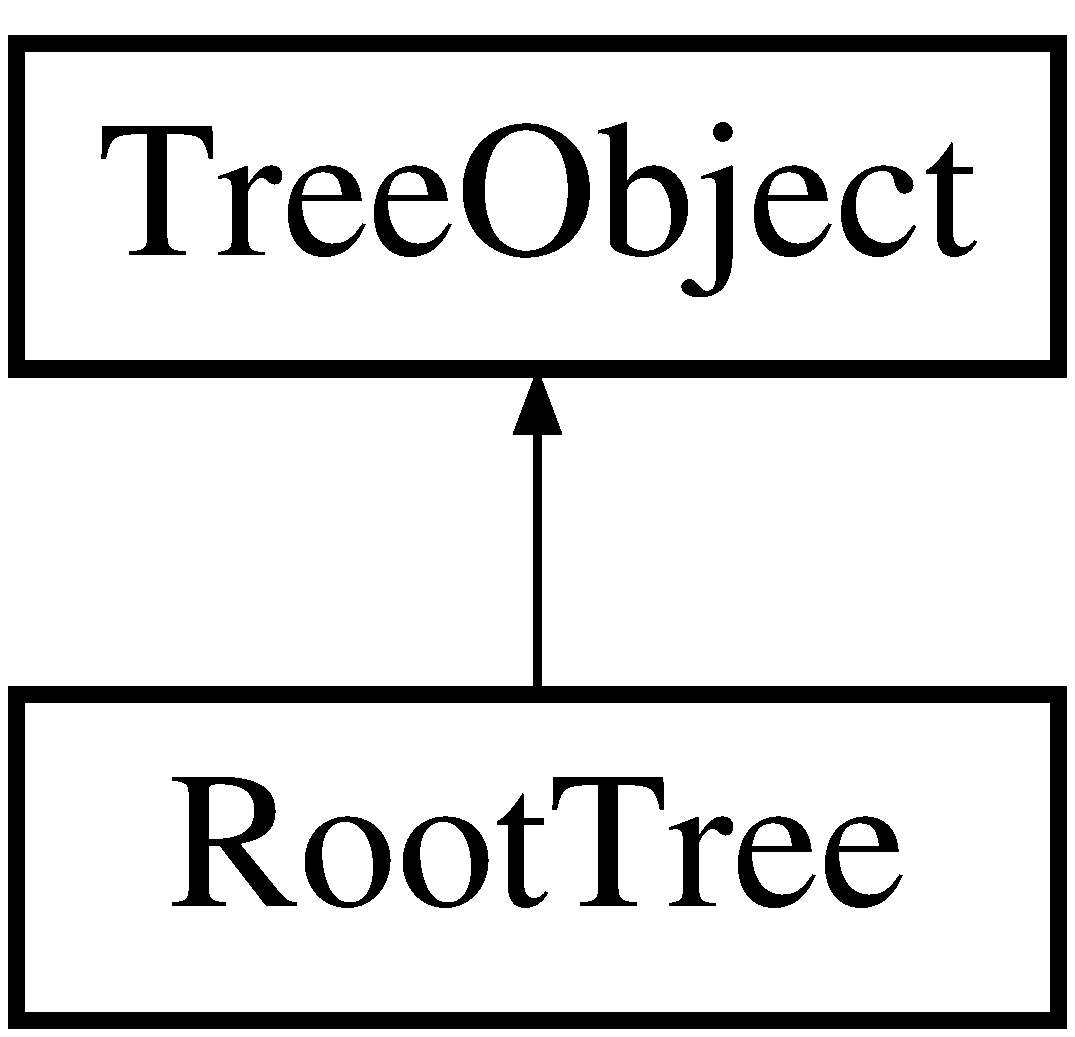
\includegraphics[height=2.000000cm]{class_root_tree}
\end{center}
\end{figure}
\subsection*{Public Member Functions}
\begin{DoxyCompactItemize}
\item 
\mbox{\hyperlink{class_root_tree_a491c0374c9024faf1e1c8045f21a4cad}{Root\+Tree}} (\mbox{\hyperlink{class_partition_manager}{Partition\+Manager}} $\ast$pm)
\item 
\mbox{\hyperlink{class_root_tree_a0e117b4a1eb94d395f9763b3cbc24916}{$\sim$\+Root\+Tree}} ()
\item 
void \mbox{\hyperlink{class_root_tree_ad6eefe5d46ee37b3725799897a78c2dd}{write\+\_\+out}} ()
\item 
void \mbox{\hyperlink{class_root_tree_a658eed78be67e890de2283af960dc532}{read\+\_\+in}} (unordered\+\_\+multimap$<$ string, \mbox{\hyperlink{class_file_info}{File\+Info}} $\ast$$>$ $\ast$all\+Files, \mbox{\hyperlink{class_root_tree}{Root\+Tree}} $\ast$root\+Tree)
\item 
void \mbox{\hyperlink{class_root_tree_ac431dc04b767fc66791c251d8173650d}{del}} ()
\end{DoxyCompactItemize}
\subsection*{Additional Inherited Members}


\subsection{Constructor \& Destructor Documentation}
\mbox{\Hypertarget{class_root_tree_a491c0374c9024faf1e1c8045f21a4cad}\label{class_root_tree_a491c0374c9024faf1e1c8045f21a4cad}} 
\index{Root\+Tree@{Root\+Tree}!Root\+Tree@{Root\+Tree}}
\index{Root\+Tree@{Root\+Tree}!Root\+Tree@{Root\+Tree}}
\subsubsection{\texorpdfstring{Root\+Tree()}{RootTree()}}
{\footnotesize\ttfamily Root\+Tree\+::\+Root\+Tree (\begin{DoxyParamCaption}\item[{\mbox{\hyperlink{class_partition_manager}{Partition\+Manager}} $\ast$}]{pm }\end{DoxyParamCaption})}


\begin{DoxyParams}{Parameters}
{\em pm} & the \mbox{\hyperlink{class_partition_manager}{Partition\+Manager}} to be associated with the \mbox{\hyperlink{class_root_tree}{Root\+Tree}} \\
\hline
\end{DoxyParams}
\mbox{\Hypertarget{class_root_tree_a0e117b4a1eb94d395f9763b3cbc24916}\label{class_root_tree_a0e117b4a1eb94d395f9763b3cbc24916}} 
\index{Root\+Tree@{Root\+Tree}!````~Root\+Tree@{$\sim$\+Root\+Tree}}
\index{````~Root\+Tree@{$\sim$\+Root\+Tree}!Root\+Tree@{Root\+Tree}}
\subsubsection{\texorpdfstring{$\sim$\+Root\+Tree()}{~RootTree()}}
{\footnotesize\ttfamily Root\+Tree\+::$\sim$\+Root\+Tree (\begin{DoxyParamCaption}{ }\end{DoxyParamCaption})}



\subsection{Member Function Documentation}
\mbox{\Hypertarget{class_root_tree_ac431dc04b767fc66791c251d8173650d}\label{class_root_tree_ac431dc04b767fc66791c251d8173650d}} 
\index{Root\+Tree@{Root\+Tree}!del@{del}}
\index{del@{del}!Root\+Tree@{Root\+Tree}}
\subsubsection{\texorpdfstring{del()}{del()}}
{\footnotesize\ttfamily void Root\+Tree\+::del (\begin{DoxyParamCaption}{ }\end{DoxyParamCaption})\hspace{0.3cm}{\ttfamily [virtual]}}

Will completely remove the \mbox{\hyperlink{class_tree_object}{Tree\+Object}}\textquotesingle{}s presence on disk 

Implements \mbox{\hyperlink{class_tree_object_af390b7479aa972888e594c07a85740b6}{Tree\+Object}}.

\mbox{\Hypertarget{class_root_tree_a658eed78be67e890de2283af960dc532}\label{class_root_tree_a658eed78be67e890de2283af960dc532}} 
\index{Root\+Tree@{Root\+Tree}!read\+\_\+in@{read\+\_\+in}}
\index{read\+\_\+in@{read\+\_\+in}!Root\+Tree@{Root\+Tree}}
\subsubsection{\texorpdfstring{read\+\_\+in()}{read\_in()}}
{\footnotesize\ttfamily void Root\+Tree\+::read\+\_\+in (\begin{DoxyParamCaption}\item[{unordered\+\_\+multimap$<$ string, \mbox{\hyperlink{class_file_info}{File\+Info}} $\ast$$>$ $\ast$}]{all\+Files,  }\item[{\mbox{\hyperlink{class_root_tree}{Root\+Tree}} $\ast$}]{root\+Tree }\end{DoxyParamCaption})\hspace{0.3cm}{\ttfamily [virtual]}}

Will read in all object data from disk 
\begin{DoxyParams}{Parameters}
{\em all\+Files} & a pointer to the map of all files \\
\hline
{\em root\+Tree} & a pointer to the root tree \\
\hline
\end{DoxyParams}


Implements \mbox{\hyperlink{class_tree_object_a722eb00e6782626281afc8eff92840a4}{Tree\+Object}}.

\mbox{\Hypertarget{class_root_tree_ad6eefe5d46ee37b3725799897a78c2dd}\label{class_root_tree_ad6eefe5d46ee37b3725799897a78c2dd}} 
\index{Root\+Tree@{Root\+Tree}!write\+\_\+out@{write\+\_\+out}}
\index{write\+\_\+out@{write\+\_\+out}!Root\+Tree@{Root\+Tree}}
\subsubsection{\texorpdfstring{write\+\_\+out()}{write\_out()}}
{\footnotesize\ttfamily void Root\+Tree\+::write\+\_\+out (\begin{DoxyParamCaption}{ }\end{DoxyParamCaption})\hspace{0.3cm}{\ttfamily [virtual]}}

Intended to write out the object to disk 

Implements \mbox{\hyperlink{class_tree_object_a63708d61353d83e3e03597394bb7aca0}{Tree\+Object}}.



The documentation for this class was generated from the following files\+:\begin{DoxyCompactItemize}
\item 
Filesystem/\+Daemon\+Dependancies/\+Trees/\mbox{\hyperlink{_trees_8h}{Trees.\+h}}\item 
Filesystem/\+Daemon\+Dependancies/\+Trees/\mbox{\hyperlink{_trees_8cpp}{Trees.\+cpp}}\end{DoxyCompactItemize}

\hypertarget{classtag__error}{}\section{tag\+\_\+error Class Reference}
\label{classtag__error}\index{tag\+\_\+error@{tag\+\_\+error}}
Inheritance diagram for tag\+\_\+error\+:\begin{figure}[H]
\begin{center}
\leavevmode
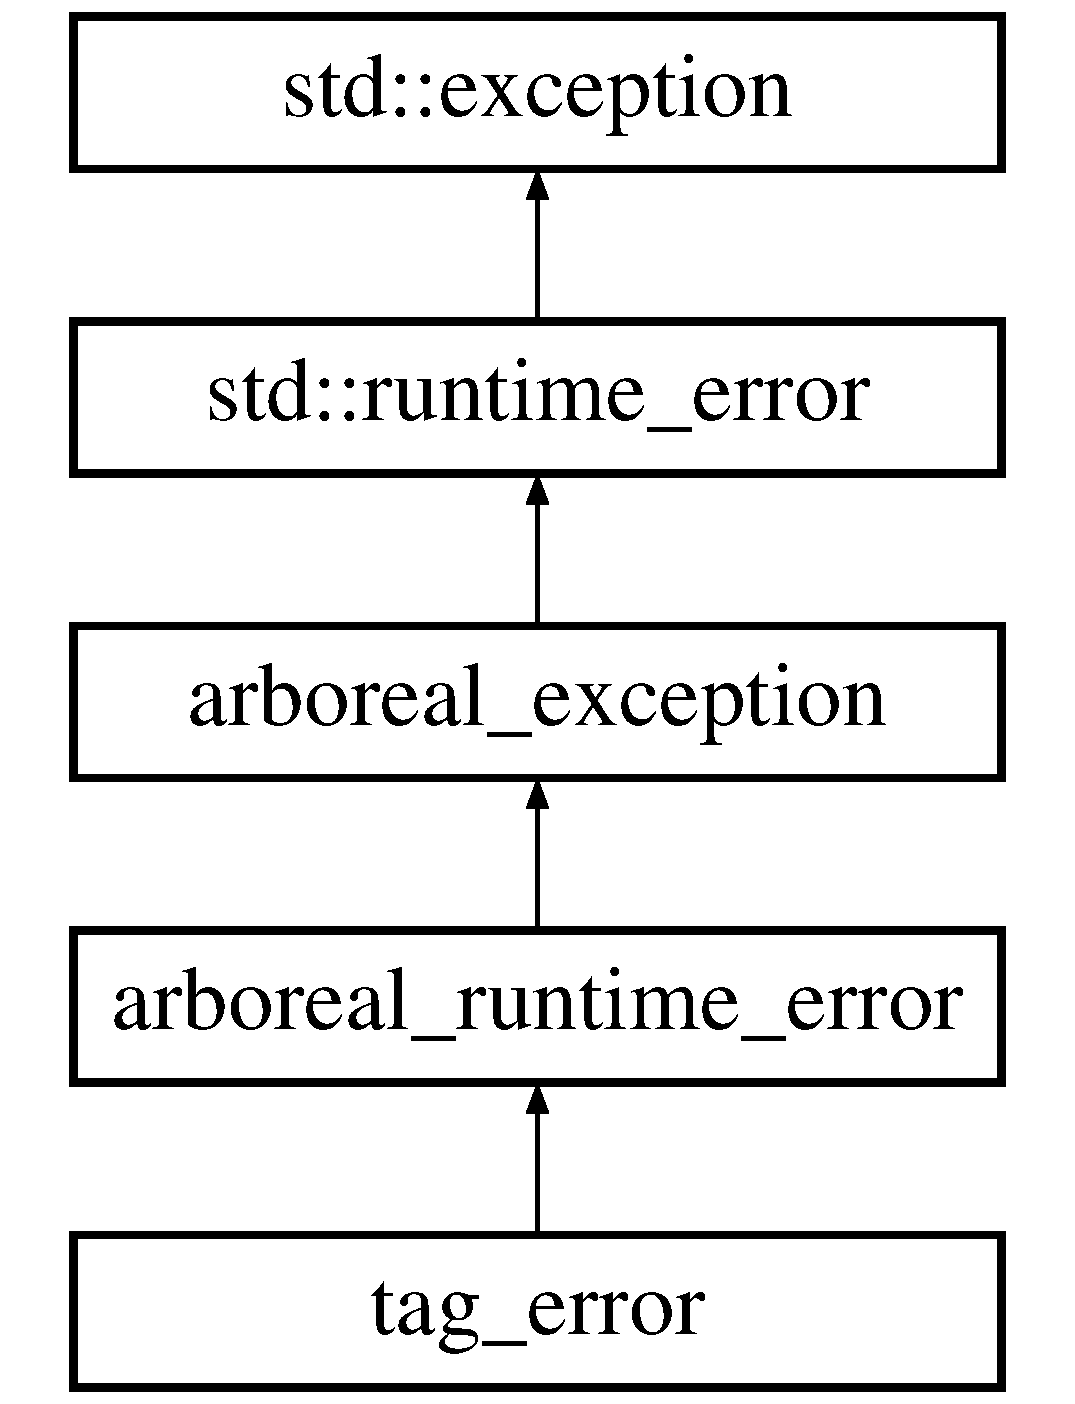
\includegraphics[height=4.000000cm]{classtag__error}
\end{center}
\end{figure}
\subsection*{Public Member Functions}
\begin{DoxyCompactItemize}
\item 
{\bfseries tag\+\_\+error} (const char $\ast$what, const char $\ast$where, const int ecode=99)\hypertarget{classtag__error_a49b7eb59916bbc065f7d79bbf31cb460}{}\label{classtag__error_a49b7eb59916bbc065f7d79bbf31cb460}

\item 
{\bfseries tag\+\_\+error} (const char $\ast$what, const string \&where, const int ecode=99)\hypertarget{classtag__error_abc7794a3cf421776f77b781b4bef9dfb}{}\label{classtag__error_abc7794a3cf421776f77b781b4bef9dfb}

\item 
{\bfseries tag\+\_\+error} (const string \&what, const string \&where, const int ecode=99)\hypertarget{classtag__error_afc103fa30ef508088c2cb4eda60837d2}{}\label{classtag__error_afc103fa30ef508088c2cb4eda60837d2}

\item 
{\bfseries tag\+\_\+error} (const string \&what, const char $\ast$where, const int ecode=99)\hypertarget{classtag__error_a70a4e7f9da04ca034f23e42ce1e95433}{}\label{classtag__error_a70a4e7f9da04ca034f23e42ce1e95433}

\end{DoxyCompactItemize}
\subsection*{Additional Inherited Members}


The documentation for this class was generated from the following files\+:\begin{DoxyCompactItemize}
\item 
Shared\+Headers/Arboreal\+\_\+\+Exceptions.\+h\item 
Shared\+C\+P\+P\+Files/Arboreal\+\_\+\+Exceptions.\+cpp\end{DoxyCompactItemize}

\hypertarget{class_tag_tree}{}\section{Tag\+Tree Class Reference}
\label{class_tag_tree}\index{Tag\+Tree@{Tag\+Tree}}


{\ttfamily \#include $<$Trees.\+h$>$}

Inheritance diagram for Tag\+Tree\+:\begin{figure}[H]
\begin{center}
\leavevmode
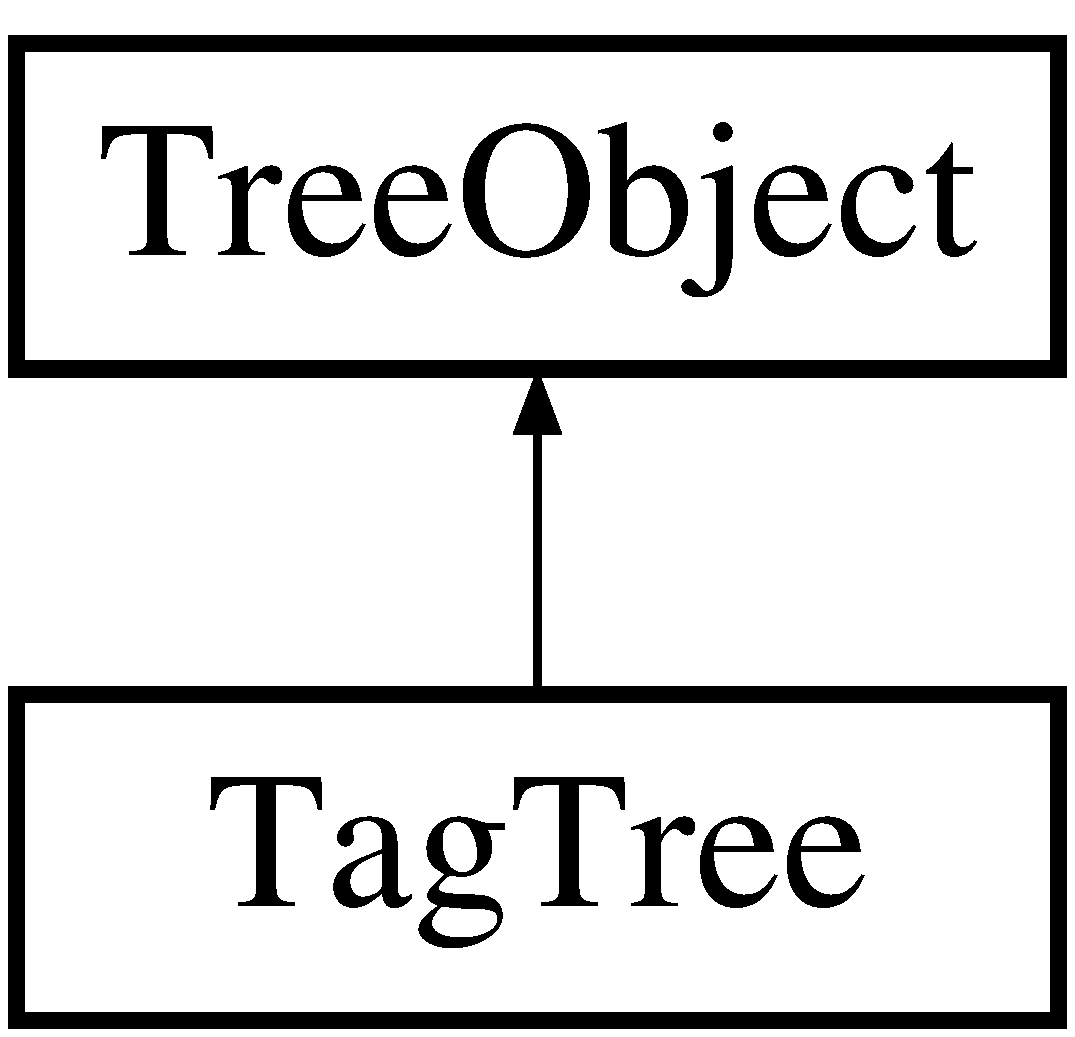
\includegraphics[height=2.000000cm]{class_tag_tree}
\end{center}
\end{figure}
\subsection*{Public Member Functions}
\begin{DoxyCompactItemize}
\item 
\mbox{\hyperlink{class_tag_tree_a80b23fa47a18727a248c3db1e8b2ed83}{Tag\+Tree}} (string tag\+Name, Blk\+Num\+Type blknum, \mbox{\hyperlink{class_partition_manager}{Partition\+Manager}} $\ast$pm)
\item 
\mbox{\hyperlink{class_tag_tree_a0522ae8933fa3e903fc1da7bdfb5d901}{$\sim$\+Tag\+Tree}} ()
\item 
void \mbox{\hyperlink{class_tag_tree_adf13e01b25991ecfef1ad958e02c07fe}{write\+\_\+out}} ()
\item 
void \mbox{\hyperlink{class_tag_tree_af86ee6713fa03c3909e04608512b8b62}{read\+\_\+in}} (unordered\+\_\+multimap$<$ string, \mbox{\hyperlink{class_file_info}{File\+Info}} $\ast$$>$ $\ast$all\+Files, \mbox{\hyperlink{class_root_tree}{Root\+Tree}} $\ast$root\+Tree)
\item 
void \mbox{\hyperlink{class_tag_tree_ad8108969f4d28b938e55c8339f19db35}{del}} ()
\end{DoxyCompactItemize}
\subsection*{Additional Inherited Members}


\subsection{Constructor \& Destructor Documentation}
\mbox{\Hypertarget{class_tag_tree_a80b23fa47a18727a248c3db1e8b2ed83}\label{class_tag_tree_a80b23fa47a18727a248c3db1e8b2ed83}} 
\index{Tag\+Tree@{Tag\+Tree}!Tag\+Tree@{Tag\+Tree}}
\index{Tag\+Tree@{Tag\+Tree}!Tag\+Tree@{Tag\+Tree}}
\subsubsection{\texorpdfstring{Tag\+Tree()}{TagTree()}}
{\footnotesize\ttfamily Tag\+Tree\+::\+Tag\+Tree (\begin{DoxyParamCaption}\item[{string}]{tag\+Name,  }\item[{Blk\+Num\+Type}]{blknum,  }\item[{\mbox{\hyperlink{class_partition_manager}{Partition\+Manager}} $\ast$}]{pm }\end{DoxyParamCaption})}


\begin{DoxyParams}{Parameters}
{\em tag\+Name} & the name of this tag \\
\hline
{\em blknum} & the blocknumber for the superblock of this tag\+Tree \\
\hline
\end{DoxyParams}
\mbox{\Hypertarget{class_tag_tree_a0522ae8933fa3e903fc1da7bdfb5d901}\label{class_tag_tree_a0522ae8933fa3e903fc1da7bdfb5d901}} 
\index{Tag\+Tree@{Tag\+Tree}!````~Tag\+Tree@{$\sim$\+Tag\+Tree}}
\index{````~Tag\+Tree@{$\sim$\+Tag\+Tree}!Tag\+Tree@{Tag\+Tree}}
\subsubsection{\texorpdfstring{$\sim$\+Tag\+Tree()}{~TagTree()}}
{\footnotesize\ttfamily Tag\+Tree\+::$\sim$\+Tag\+Tree (\begin{DoxyParamCaption}{ }\end{DoxyParamCaption})}



\subsection{Member Function Documentation}
\mbox{\Hypertarget{class_tag_tree_ad8108969f4d28b938e55c8339f19db35}\label{class_tag_tree_ad8108969f4d28b938e55c8339f19db35}} 
\index{Tag\+Tree@{Tag\+Tree}!del@{del}}
\index{del@{del}!Tag\+Tree@{Tag\+Tree}}
\subsubsection{\texorpdfstring{del()}{del()}}
{\footnotesize\ttfamily void Tag\+Tree\+::del (\begin{DoxyParamCaption}{ }\end{DoxyParamCaption})\hspace{0.3cm}{\ttfamily [virtual]}}

Will completely remove the \mbox{\hyperlink{class_tree_object}{Tree\+Object}}\textquotesingle{}s presence on disk 

Implements \mbox{\hyperlink{class_tree_object_af390b7479aa972888e594c07a85740b6}{Tree\+Object}}.

\mbox{\Hypertarget{class_tag_tree_af86ee6713fa03c3909e04608512b8b62}\label{class_tag_tree_af86ee6713fa03c3909e04608512b8b62}} 
\index{Tag\+Tree@{Tag\+Tree}!read\+\_\+in@{read\+\_\+in}}
\index{read\+\_\+in@{read\+\_\+in}!Tag\+Tree@{Tag\+Tree}}
\subsubsection{\texorpdfstring{read\+\_\+in()}{read\_in()}}
{\footnotesize\ttfamily void Tag\+Tree\+::read\+\_\+in (\begin{DoxyParamCaption}\item[{unordered\+\_\+multimap$<$ string, \mbox{\hyperlink{class_file_info}{File\+Info}} $\ast$$>$ $\ast$}]{all\+Files,  }\item[{\mbox{\hyperlink{class_root_tree}{Root\+Tree}} $\ast$}]{root\+Tree }\end{DoxyParamCaption})\hspace{0.3cm}{\ttfamily [virtual]}}

Will read in all object data from disk 
\begin{DoxyParams}{Parameters}
{\em all\+Files} & a pointer to the map of all files \\
\hline
{\em root\+Tree} & a pointer to the root tree \\
\hline
\end{DoxyParams}


Implements \mbox{\hyperlink{class_tree_object_a722eb00e6782626281afc8eff92840a4}{Tree\+Object}}.

\mbox{\Hypertarget{class_tag_tree_adf13e01b25991ecfef1ad958e02c07fe}\label{class_tag_tree_adf13e01b25991ecfef1ad958e02c07fe}} 
\index{Tag\+Tree@{Tag\+Tree}!write\+\_\+out@{write\+\_\+out}}
\index{write\+\_\+out@{write\+\_\+out}!Tag\+Tree@{Tag\+Tree}}
\subsubsection{\texorpdfstring{write\+\_\+out()}{write\_out()}}
{\footnotesize\ttfamily void Tag\+Tree\+::write\+\_\+out (\begin{DoxyParamCaption}{ }\end{DoxyParamCaption})\hspace{0.3cm}{\ttfamily [virtual]}}

Intended to write out the object to disk 

Implements \mbox{\hyperlink{class_tree_object_a63708d61353d83e3e03597394bb7aca0}{Tree\+Object}}.



The documentation for this class was generated from the following files\+:\begin{DoxyCompactItemize}
\item 
Filesystem/\+Daemon\+Dependancies/\+Trees/\mbox{\hyperlink{_trees_8h}{Trees.\+h}}\item 
Filesystem/\+Daemon\+Dependancies/\+Trees/\mbox{\hyperlink{_trees_8cpp}{Trees.\+cpp}}\end{DoxyCompactItemize}

\hypertarget{class_tree_object}{}\section{Tree\+Object Class Reference}
\label{class_tree_object}\index{Tree\+Object@{Tree\+Object}}


{\ttfamily \#include $<$Trees.\+h$>$}

Inheritance diagram for Tree\+Object\+:\begin{figure}[H]
\begin{center}
\leavevmode
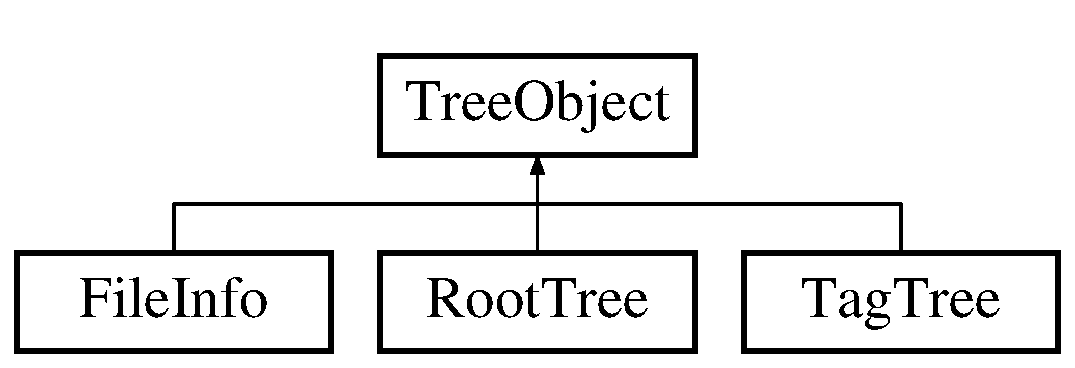
\includegraphics[height=2.000000cm]{class_tree_object}
\end{center}
\end{figure}
\subsection*{Public Member Functions}
\begin{DoxyCompactItemize}
\item 
virtual \mbox{\hyperlink{class_tree_object_a0be0e98771c0ccbeee1930c340d372a9}{$\sim$\+Tree\+Object}} ()
\item 
\mbox{\hyperlink{class_tree_object_a1ef90156e6b45ddef28c59a89cd1097d}{Tree\+Object}} (string name, Blk\+Num\+Type blknum, \mbox{\hyperlink{class_partition_manager}{Partition\+Manager}} $\ast$pm)
\end{DoxyCompactItemize}
\begin{Indent}\textbf{ Accessor Functions}\par
\begin{DoxyCompactItemize}
\item 
string \mbox{\hyperlink{class_tree_object_a5216922ec0b98bcc375601db8d253770}{get\+\_\+name}} () const
\item 
Blk\+Num\+Type \mbox{\hyperlink{class_tree_object_af7841065fe85d0884341d72669185169}{get\+\_\+block\+\_\+number}} () const
\item 
Index \mbox{\hyperlink{class_tree_object_ae0983a3ff99d413e22beaaac8d7b6d12}{get\+\_\+index}} (\mbox{\hyperlink{class_tree_object}{Tree\+Object}} $\ast$obj) const
\item 
Index \mbox{\hyperlink{class_tree_object_a2d7c1a4c2d36c81110ccae09d9724125}{get\+\_\+last\+\_\+entry}} () const
\item 
Blk\+Num\+Type \mbox{\hyperlink{class_tree_object_a16153734dbee4adc99fa195715728c2f}{get\+\_\+start\+\_\+block}} () const
\item 
size\+\_\+t \mbox{\hyperlink{class_tree_object_a2a3dffe29aba8965c7977312c3721b50}{size}} () const
\item 
unordered\+\_\+map$<$ string, \mbox{\hyperlink{class_tree_object}{Tree\+Object}} $\ast$ $>$\+::iterator \mbox{\hyperlink{class_tree_object_af8bb5e54c0a13e1e0e5be409153ab6d8}{begin}} ()
\item 
unordered\+\_\+map$<$ string, \mbox{\hyperlink{class_tree_object}{Tree\+Object}} $\ast$ $>$\+::iterator \mbox{\hyperlink{class_tree_object_a2544e2976f3b75cd1f0230f5f908059c}{end}} ()
\item 
\mbox{\hyperlink{class_tree_object}{Tree\+Object}} $\ast$ \mbox{\hyperlink{class_tree_object_a6a7477c29a06a9896df549f83611252f}{find}} (string name) const
\item 
queue$<$ Index $>$ $\ast$ \mbox{\hyperlink{class_tree_object_aa0900ad50c10023e4700f11218d30d7a}{get\+\_\+free\+\_\+spots}} ()
\end{DoxyCompactItemize}
\end{Indent}
\begin{Indent}\textbf{ Modifier Functions}\par
\begin{DoxyCompactItemize}
\item 
void \mbox{\hyperlink{class_tree_object_a8ae7e42502b4652102e0b3c4c4e1671b}{set\+\_\+name}} (string name)
\item 
void \mbox{\hyperlink{class_tree_object_af908239ff96a0f3064d0d8aefb58381b}{add\+\_\+index}} (\mbox{\hyperlink{class_tree_object}{Tree\+Object}} $\ast$obj, Index index)
\item 
void \mbox{\hyperlink{class_tree_object_a2ec94bc9d2647275049ddf2a70b8510e}{set\+\_\+last\+\_\+entry}} (Index index)
\item 
virtual void \mbox{\hyperlink{class_tree_object_af8cc57edba9f435b52ccf33cfbbb2fc6}{insert}} (string name, \mbox{\hyperlink{class_tree_object}{Tree\+Object}} $\ast$obj)
\item 
virtual void \mbox{\hyperlink{class_tree_object_a453b5df2a9ef7c6faad259900d574ee2}{erase}} (string name)
\item 
virtual void \mbox{\hyperlink{class_tree_object_a41ce6080e0df5adcea4b0a76d35af885}{insert\+\_\+addition}} (\mbox{\hyperlink{class_tree_object}{Tree\+Object}} $\ast$add)
\item 
virtual void \mbox{\hyperlink{class_tree_object_afcc4b3928d2b77ff080aa229a9706215}{insert\+\_\+deletion}} (\mbox{\hyperlink{class_tree_object}{Tree\+Object}} $\ast$\mbox{\hyperlink{class_tree_object_af390b7479aa972888e594c07a85740b6}{del}})
\end{DoxyCompactItemize}
\end{Indent}
\begin{Indent}\textbf{ Disk Functions}\par
\begin{DoxyCompactItemize}
\item 
virtual void \mbox{\hyperlink{class_tree_object_a63708d61353d83e3e03597394bb7aca0}{write\+\_\+out}} ()=0
\item 
virtual void \mbox{\hyperlink{class_tree_object_a722eb00e6782626281afc8eff92840a4}{read\+\_\+in}} (unordered\+\_\+multimap$<$ string, \mbox{\hyperlink{class_file_info}{File\+Info}} $\ast$$>$ $\ast$all\+Files, \mbox{\hyperlink{class_root_tree}{Root\+Tree}} $\ast$root\+Tree)=0
\item 
virtual void \mbox{\hyperlink{class_tree_object_af390b7479aa972888e594c07a85740b6}{del}} ()=0
\item 
void \mbox{\hyperlink{class_tree_object_a6b6f0a5c23577748b489652013fa1728}{increment\+\_\+allocate}} (Index $\ast$index)
\item 
void \mbox{\hyperlink{class_tree_object_a86fbde9e7ee245385bf7ca7a8f355bd0}{increment\+\_\+follow}} (Index $\ast$index)
\end{DoxyCompactItemize}
\end{Indent}
\subsection*{Protected Member Functions}
\begin{DoxyCompactItemize}
\item 
virtual void \mbox{\hyperlink{class_tree_object_a07f5f5de1cff0cfdc2372e81559f5181}{delete\+\_\+cont\+\_\+blocks}} (Blk\+Num\+Type blknum)
\end{DoxyCompactItemize}
\subsection*{Protected Attributes}
\begin{DoxyCompactItemize}
\item 
queue$<$ \mbox{\hyperlink{class_modification}{Modification}} $\ast$ $>$ \mbox{\hyperlink{class_tree_object_ac285793f5d7cba8069670210606c66c7}{\+\_\+modifications}}
\begin{DoxyCompactList}\small\item\em A collection of associated Modifications. \end{DoxyCompactList}\item 
unordered\+\_\+map$<$ string, \mbox{\hyperlink{class_tree_object}{Tree\+Object}} $\ast$ $>$ \mbox{\hyperlink{class_tree_object_a59effca19a3475c84496c7f82c856d38}{\+\_\+my\+Tree}}
\begin{DoxyCompactList}\small\item\em A collection of contained Tree\+Objects. \end{DoxyCompactList}\item 
string \mbox{\hyperlink{class_tree_object_a368b410ed9b21c7106babf2ba93399b3}{\+\_\+name}}
\begin{DoxyCompactList}\small\item\em name or value \end{DoxyCompactList}\item 
Blk\+Num\+Type \mbox{\hyperlink{class_tree_object_a17cfa5bde700978b4ec326909362bd2c}{\+\_\+block\+Number}}
\begin{DoxyCompactList}\small\item\em Blocknumber of the superblock on disk. \end{DoxyCompactList}\item 
unordered\+\_\+map$<$ \mbox{\hyperlink{class_tree_object}{Tree\+Object}} $\ast$, Index $>$ \mbox{\hyperlink{class_tree_object_ae79eb5bd12c820b50f5d10c3f9b5dc66}{\+\_\+indeces}}
\begin{DoxyCompactList}\small\item\em location(s) of the superblock entry(ies) on disk \end{DoxyCompactList}\item 
Index \mbox{\hyperlink{class_tree_object_a1418b7078e9fbb06506a310ad9417c52}{\+\_\+last\+Entry}}
\begin{DoxyCompactList}\small\item\em Index of the last entry of data on disk. \end{DoxyCompactList}\item 
Blk\+Num\+Type \mbox{\hyperlink{class_tree_object_a5872ffdaa0c1a0cbf393da9a8a7657f3}{\+\_\+start\+Block}}
\begin{DoxyCompactList}\small\item\em blocknumber of the start of this data on disk \end{DoxyCompactList}\item 
\mbox{\hyperlink{class_partition_manager}{Partition\+Manager}} $\ast$ \mbox{\hyperlink{class_tree_object_a0b2ab130a5b95945bbd81250f667d63b}{\+\_\+my\+Partition\+Manager}}
\begin{DoxyCompactList}\small\item\em Associated \mbox{\hyperlink{class_partition_manager}{Partition\+Manager}}. \end{DoxyCompactList}\item 
queue$<$ Index $>$ \mbox{\hyperlink{class_tree_object_a43defc5d87c903cdc3e36edc3323ef87}{\+\_\+free\+Spots}}
\end{DoxyCompactItemize}


\subsection{Constructor \& Destructor Documentation}
\mbox{\Hypertarget{class_tree_object_a0be0e98771c0ccbeee1930c340d372a9}\label{class_tree_object_a0be0e98771c0ccbeee1930c340d372a9}} 
\index{Tree\+Object@{Tree\+Object}!````~Tree\+Object@{$\sim$\+Tree\+Object}}
\index{````~Tree\+Object@{$\sim$\+Tree\+Object}!Tree\+Object@{Tree\+Object}}
\subsubsection{\texorpdfstring{$\sim$\+Tree\+Object()}{~TreeObject()}}
{\footnotesize\ttfamily Tree\+Object\+::$\sim$\+Tree\+Object (\begin{DoxyParamCaption}{ }\end{DoxyParamCaption})\hspace{0.3cm}{\ttfamily [virtual]}}

\mbox{\Hypertarget{class_tree_object_a1ef90156e6b45ddef28c59a89cd1097d}\label{class_tree_object_a1ef90156e6b45ddef28c59a89cd1097d}} 
\index{Tree\+Object@{Tree\+Object}!Tree\+Object@{Tree\+Object}}
\index{Tree\+Object@{Tree\+Object}!Tree\+Object@{Tree\+Object}}
\subsubsection{\texorpdfstring{Tree\+Object()}{TreeObject()}}
{\footnotesize\ttfamily Tree\+Object\+::\+Tree\+Object (\begin{DoxyParamCaption}\item[{string}]{name,  }\item[{Blk\+Num\+Type}]{blknum,  }\item[{\mbox{\hyperlink{class_partition_manager}{Partition\+Manager}} $\ast$}]{pm }\end{DoxyParamCaption})}


\begin{DoxyParams}{Parameters}
{\em name} & name of this object \\
\hline
{\em blknum} & blocknumber of the superblock \\
\hline
{\em pm} & \mbox{\hyperlink{class_partition_manager}{Partition\+Manager}} object to be associated with this object \\
\hline
\end{DoxyParams}


\subsection{Member Function Documentation}
\mbox{\Hypertarget{class_tree_object_af908239ff96a0f3064d0d8aefb58381b}\label{class_tree_object_af908239ff96a0f3064d0d8aefb58381b}} 
\index{Tree\+Object@{Tree\+Object}!add\+\_\+index@{add\+\_\+index}}
\index{add\+\_\+index@{add\+\_\+index}!Tree\+Object@{Tree\+Object}}
\subsubsection{\texorpdfstring{add\+\_\+index()}{add\_index()}}
{\footnotesize\ttfamily void Tree\+Object\+::add\+\_\+index (\begin{DoxyParamCaption}\item[{\mbox{\hyperlink{class_tree_object}{Tree\+Object}} $\ast$}]{obj,  }\item[{Index}]{index }\end{DoxyParamCaption})}

Add an index to \+\_\+indeces for the specified \mbox{\hyperlink{class_tree_object}{Tree\+Object}}. If the index already existed. nothing happpens 
\begin{DoxyParams}{Parameters}
{\em obj} & the object that the Index references to \\
\hline
{\em index} & the Index of obj \\
\hline
\end{DoxyParams}
\mbox{\Hypertarget{class_tree_object_af8bb5e54c0a13e1e0e5be409153ab6d8}\label{class_tree_object_af8bb5e54c0a13e1e0e5be409153ab6d8}} 
\index{Tree\+Object@{Tree\+Object}!begin@{begin}}
\index{begin@{begin}!Tree\+Object@{Tree\+Object}}
\subsubsection{\texorpdfstring{begin()}{begin()}}
{\footnotesize\ttfamily unordered\+\_\+map$<$ string, \mbox{\hyperlink{class_tree_object}{Tree\+Object}} $\ast$ $>$\+::iterator Tree\+Object\+::begin (\begin{DoxyParamCaption}{ }\end{DoxyParamCaption})}

\begin{DoxyReturn}{Returns}
An iterator to the beginning of the Tree\+Objects associated with this object 
\end{DoxyReturn}
\mbox{\Hypertarget{class_tree_object_af390b7479aa972888e594c07a85740b6}\label{class_tree_object_af390b7479aa972888e594c07a85740b6}} 
\index{Tree\+Object@{Tree\+Object}!del@{del}}
\index{del@{del}!Tree\+Object@{Tree\+Object}}
\subsubsection{\texorpdfstring{del()}{del()}}
{\footnotesize\ttfamily virtual void Tree\+Object\+::del (\begin{DoxyParamCaption}{ }\end{DoxyParamCaption})\hspace{0.3cm}{\ttfamily [pure virtual]}}

Will completely remove the \mbox{\hyperlink{class_tree_object}{Tree\+Object}}\textquotesingle{}s presence on disk 

Implemented in \mbox{\hyperlink{class_root_tree_ac431dc04b767fc66791c251d8173650d}{Root\+Tree}}, \mbox{\hyperlink{class_tag_tree_ad8108969f4d28b938e55c8339f19db35}{Tag\+Tree}}, and \mbox{\hyperlink{class_file_info_a2ca34d945ed1208f227a249ba72ee427}{File\+Info}}.

\mbox{\Hypertarget{class_tree_object_a07f5f5de1cff0cfdc2372e81559f5181}\label{class_tree_object_a07f5f5de1cff0cfdc2372e81559f5181}} 
\index{Tree\+Object@{Tree\+Object}!delete\+\_\+cont\+\_\+blocks@{delete\+\_\+cont\+\_\+blocks}}
\index{delete\+\_\+cont\+\_\+blocks@{delete\+\_\+cont\+\_\+blocks}!Tree\+Object@{Tree\+Object}}
\subsubsection{\texorpdfstring{delete\+\_\+cont\+\_\+blocks()}{delete\_cont\_blocks()}}
{\footnotesize\ttfamily void Tree\+Object\+::delete\+\_\+cont\+\_\+blocks (\begin{DoxyParamCaption}\item[{Blk\+Num\+Type}]{blknum }\end{DoxyParamCaption})\hspace{0.3cm}{\ttfamily [protected]}, {\ttfamily [virtual]}}

Will follow the chain of continuation blocks and free all of them 
\begin{DoxyParams}{Parameters}
{\em blknum} & will free the blknum and use it to follow the chain of continuation blocks \\
\hline
\end{DoxyParams}


Reimplemented in \mbox{\hyperlink{class_file_info_a8c6b58cb9f7e9978064291ef81380e01}{File\+Info}}.

\mbox{\Hypertarget{class_tree_object_a2544e2976f3b75cd1f0230f5f908059c}\label{class_tree_object_a2544e2976f3b75cd1f0230f5f908059c}} 
\index{Tree\+Object@{Tree\+Object}!end@{end}}
\index{end@{end}!Tree\+Object@{Tree\+Object}}
\subsubsection{\texorpdfstring{end()}{end()}}
{\footnotesize\ttfamily unordered\+\_\+map$<$ string, \mbox{\hyperlink{class_tree_object}{Tree\+Object}} $\ast$ $>$\+::iterator Tree\+Object\+::end (\begin{DoxyParamCaption}{ }\end{DoxyParamCaption})}

\begin{DoxyReturn}{Returns}
An iterator to the end of the Tree\+Objects associated with this object 
\end{DoxyReturn}
\mbox{\Hypertarget{class_tree_object_a453b5df2a9ef7c6faad259900d574ee2}\label{class_tree_object_a453b5df2a9ef7c6faad259900d574ee2}} 
\index{Tree\+Object@{Tree\+Object}!erase@{erase}}
\index{erase@{erase}!Tree\+Object@{Tree\+Object}}
\subsubsection{\texorpdfstring{erase()}{erase()}}
{\footnotesize\ttfamily void Tree\+Object\+::erase (\begin{DoxyParamCaption}\item[{string}]{name }\end{DoxyParamCaption})\hspace{0.3cm}{\ttfamily [virtual]}}

Disassociate the given name from this object 
\begin{DoxyParams}{Parameters}
{\em name} & the name of the object to be erased. \\
\hline
\end{DoxyParams}

\begin{DoxyExceptions}{Exceptions}
{\em \mbox{\hyperlink{classarboreal__logic__error}{arboreal\+\_\+logic\+\_\+error}}} & \\
\hline
\end{DoxyExceptions}


Reimplemented in \mbox{\hyperlink{class_file_info_ae058242283d3317eaf2b79428e6137f6}{File\+Info}}.

\mbox{\Hypertarget{class_tree_object_a6a7477c29a06a9896df549f83611252f}\label{class_tree_object_a6a7477c29a06a9896df549f83611252f}} 
\index{Tree\+Object@{Tree\+Object}!find@{find}}
\index{find@{find}!Tree\+Object@{Tree\+Object}}
\subsubsection{\texorpdfstring{find()}{find()}}
{\footnotesize\ttfamily \mbox{\hyperlink{class_tree_object}{Tree\+Object}} $\ast$ Tree\+Object\+::find (\begin{DoxyParamCaption}\item[{string}]{name }\end{DoxyParamCaption}) const}

Search \+\_\+my\+Tree for the specified name 
\begin{DoxyParams}{Parameters}
{\em name} & the name of the desired object \\
\hline
\end{DoxyParams}
\begin{DoxyReturn}{Returns}
a pointer to the object if found, 0 otherwise 
\end{DoxyReturn}
\mbox{\Hypertarget{class_tree_object_af7841065fe85d0884341d72669185169}\label{class_tree_object_af7841065fe85d0884341d72669185169}} 
\index{Tree\+Object@{Tree\+Object}!get\+\_\+block\+\_\+number@{get\+\_\+block\+\_\+number}}
\index{get\+\_\+block\+\_\+number@{get\+\_\+block\+\_\+number}!Tree\+Object@{Tree\+Object}}
\subsubsection{\texorpdfstring{get\+\_\+block\+\_\+number()}{get\_block\_number()}}
{\footnotesize\ttfamily Blk\+Num\+Type Tree\+Object\+::get\+\_\+block\+\_\+number (\begin{DoxyParamCaption}{ }\end{DoxyParamCaption}) const}

\begin{DoxyReturn}{Returns}
The blocknumber of the superblock 
\end{DoxyReturn}
\mbox{\Hypertarget{class_tree_object_aa0900ad50c10023e4700f11218d30d7a}\label{class_tree_object_aa0900ad50c10023e4700f11218d30d7a}} 
\index{Tree\+Object@{Tree\+Object}!get\+\_\+free\+\_\+spots@{get\+\_\+free\+\_\+spots}}
\index{get\+\_\+free\+\_\+spots@{get\+\_\+free\+\_\+spots}!Tree\+Object@{Tree\+Object}}
\subsubsection{\texorpdfstring{get\+\_\+free\+\_\+spots()}{get\_free\_spots()}}
{\footnotesize\ttfamily queue$<$ Index $>$ $\ast$ Tree\+Object\+::get\+\_\+free\+\_\+spots (\begin{DoxyParamCaption}{ }\end{DoxyParamCaption})}

\begin{DoxyReturn}{Returns}
a pointer to the queue of empty spaces where new entries can be added 
\end{DoxyReturn}
\mbox{\Hypertarget{class_tree_object_ae0983a3ff99d413e22beaaac8d7b6d12}\label{class_tree_object_ae0983a3ff99d413e22beaaac8d7b6d12}} 
\index{Tree\+Object@{Tree\+Object}!get\+\_\+index@{get\+\_\+index}}
\index{get\+\_\+index@{get\+\_\+index}!Tree\+Object@{Tree\+Object}}
\subsubsection{\texorpdfstring{get\+\_\+index()}{get\_index()}}
{\footnotesize\ttfamily Index Tree\+Object\+::get\+\_\+index (\begin{DoxyParamCaption}\item[{\mbox{\hyperlink{class_tree_object}{Tree\+Object}} $\ast$}]{obj }\end{DoxyParamCaption}) const}

Searches for obj and returns the Index of obj on disk, if found 
\begin{DoxyParams}{Parameters}
{\em obj} & object whose position is desired \\
\hline
\end{DoxyParams}
\begin{DoxyReturn}{Returns}
The Index of obj on disk, 
\end{DoxyReturn}

\begin{DoxyExceptions}{Exceptions}
{\em \mbox{\hyperlink{classarboreal__logic__error}{arboreal\+\_\+logic\+\_\+error}}} & \\
\hline
\end{DoxyExceptions}
\mbox{\Hypertarget{class_tree_object_a2d7c1a4c2d36c81110ccae09d9724125}\label{class_tree_object_a2d7c1a4c2d36c81110ccae09d9724125}} 
\index{Tree\+Object@{Tree\+Object}!get\+\_\+last\+\_\+entry@{get\+\_\+last\+\_\+entry}}
\index{get\+\_\+last\+\_\+entry@{get\+\_\+last\+\_\+entry}!Tree\+Object@{Tree\+Object}}
\subsubsection{\texorpdfstring{get\+\_\+last\+\_\+entry()}{get\_last\_entry()}}
{\footnotesize\ttfamily Index Tree\+Object\+::get\+\_\+last\+\_\+entry (\begin{DoxyParamCaption}{ }\end{DoxyParamCaption}) const}

Find the Index of the last entry for this object on disk \begin{DoxyReturn}{Returns}
Index of the last entry on disk 
\end{DoxyReturn}
\mbox{\Hypertarget{class_tree_object_a5216922ec0b98bcc375601db8d253770}\label{class_tree_object_a5216922ec0b98bcc375601db8d253770}} 
\index{Tree\+Object@{Tree\+Object}!get\+\_\+name@{get\+\_\+name}}
\index{get\+\_\+name@{get\+\_\+name}!Tree\+Object@{Tree\+Object}}
\subsubsection{\texorpdfstring{get\+\_\+name()}{get\_name()}}
{\footnotesize\ttfamily string Tree\+Object\+::get\+\_\+name (\begin{DoxyParamCaption}{ }\end{DoxyParamCaption}) const}

\begin{DoxyReturn}{Returns}
The name 
\end{DoxyReturn}
\mbox{\Hypertarget{class_tree_object_a16153734dbee4adc99fa195715728c2f}\label{class_tree_object_a16153734dbee4adc99fa195715728c2f}} 
\index{Tree\+Object@{Tree\+Object}!get\+\_\+start\+\_\+block@{get\+\_\+start\+\_\+block}}
\index{get\+\_\+start\+\_\+block@{get\+\_\+start\+\_\+block}!Tree\+Object@{Tree\+Object}}
\subsubsection{\texorpdfstring{get\+\_\+start\+\_\+block()}{get\_start\_block()}}
{\footnotesize\ttfamily Blk\+Num\+Type Tree\+Object\+::get\+\_\+start\+\_\+block (\begin{DoxyParamCaption}{ }\end{DoxyParamCaption}) const}

\begin{DoxyReturn}{Returns}
The start block of data for this object 
\end{DoxyReturn}
\mbox{\Hypertarget{class_tree_object_a6b6f0a5c23577748b489652013fa1728}\label{class_tree_object_a6b6f0a5c23577748b489652013fa1728}} 
\index{Tree\+Object@{Tree\+Object}!increment\+\_\+allocate@{increment\+\_\+allocate}}
\index{increment\+\_\+allocate@{increment\+\_\+allocate}!Tree\+Object@{Tree\+Object}}
\subsubsection{\texorpdfstring{increment\+\_\+allocate()}{increment\_allocate()}}
{\footnotesize\ttfamily void Tree\+Object\+::increment\+\_\+allocate (\begin{DoxyParamCaption}\item[{Index $\ast$}]{index }\end{DoxyParamCaption})}

Will increment the Index passed and allocate blocks if necessary to do so 
\begin{DoxyParams}{Parameters}
{\em index} & the Index to be incremented \\
\hline
\end{DoxyParams}
\mbox{\Hypertarget{class_tree_object_a86fbde9e7ee245385bf7ca7a8f355bd0}\label{class_tree_object_a86fbde9e7ee245385bf7ca7a8f355bd0}} 
\index{Tree\+Object@{Tree\+Object}!increment\+\_\+follow@{increment\+\_\+follow}}
\index{increment\+\_\+follow@{increment\+\_\+follow}!Tree\+Object@{Tree\+Object}}
\subsubsection{\texorpdfstring{increment\+\_\+follow()}{increment\_follow()}}
{\footnotesize\ttfamily void Tree\+Object\+::increment\+\_\+follow (\begin{DoxyParamCaption}\item[{Index $\ast$}]{index }\end{DoxyParamCaption})}

Will increment the Index passed but only follow the chain of already allocated blocks 
\begin{DoxyParams}{Parameters}
{\em index} & the Index to be incremented \\
\hline
\end{DoxyParams}
\mbox{\Hypertarget{class_tree_object_af8cc57edba9f435b52ccf33cfbbb2fc6}\label{class_tree_object_af8cc57edba9f435b52ccf33cfbbb2fc6}} 
\index{Tree\+Object@{Tree\+Object}!insert@{insert}}
\index{insert@{insert}!Tree\+Object@{Tree\+Object}}
\subsubsection{\texorpdfstring{insert()}{insert()}}
{\footnotesize\ttfamily void Tree\+Object\+::insert (\begin{DoxyParamCaption}\item[{string}]{name,  }\item[{\mbox{\hyperlink{class_tree_object}{Tree\+Object}} $\ast$}]{obj }\end{DoxyParamCaption})\hspace{0.3cm}{\ttfamily [virtual]}}

Associate a \mbox{\hyperlink{class_tree_object}{Tree\+Object}} with this object 
\begin{DoxyParams}{Parameters}
{\em name} & name of the object, mangled if inserting a \mbox{\hyperlink{class_file_info}{File\+Info}} \\
\hline
{\em obj} & the object to be inserted \\
\hline
\end{DoxyParams}

\begin{DoxyExceptions}{Exceptions}
{\em \mbox{\hyperlink{classtag__error}{tag\+\_\+error}}} & \\
\hline
\end{DoxyExceptions}
\begin{DoxySeeAlso}{See also}
\mbox{\hyperlink{class_file_info_ad93a84b63e417b07aa68b619051ab746}{File\+Info\+::insert()}} 
\end{DoxySeeAlso}


Reimplemented in \mbox{\hyperlink{class_file_info_ad93a84b63e417b07aa68b619051ab746}{File\+Info}}.

\mbox{\Hypertarget{class_tree_object_a41ce6080e0df5adcea4b0a76d35af885}\label{class_tree_object_a41ce6080e0df5adcea4b0a76d35af885}} 
\index{Tree\+Object@{Tree\+Object}!insert\+\_\+addition@{insert\+\_\+addition}}
\index{insert\+\_\+addition@{insert\+\_\+addition}!Tree\+Object@{Tree\+Object}}
\subsubsection{\texorpdfstring{insert\+\_\+addition()}{insert\_addition()}}
{\footnotesize\ttfamily void Tree\+Object\+::insert\+\_\+addition (\begin{DoxyParamCaption}\item[{\mbox{\hyperlink{class_tree_object}{Tree\+Object}} $\ast$}]{add }\end{DoxyParamCaption})\hspace{0.3cm}{\ttfamily [virtual]}}

Add an \mbox{\hyperlink{class_addition}{Addition}} to the list of Modifications so that it can be written out later. Note\+: Do not call this on a \mbox{\hyperlink{class_file_info}{File\+Info}}. 
\begin{DoxyParams}{Parameters}
{\em add} & the object that was previously inserted to this object which will be added to the list of Modifications \\
\hline
\end{DoxyParams}
\begin{DoxySeeAlso}{See also}
File\+System\+::write\+\_\+out() \mbox{\hyperlink{class_tree_object_af8cc57edba9f435b52ccf33cfbbb2fc6}{Tree\+Object\+::insert()}} 
\end{DoxySeeAlso}


Reimplemented in \mbox{\hyperlink{class_file_info_a7f788f31521c535646eebfa9959bbb24}{File\+Info}}.

\mbox{\Hypertarget{class_tree_object_afcc4b3928d2b77ff080aa229a9706215}\label{class_tree_object_afcc4b3928d2b77ff080aa229a9706215}} 
\index{Tree\+Object@{Tree\+Object}!insert\+\_\+deletion@{insert\+\_\+deletion}}
\index{insert\+\_\+deletion@{insert\+\_\+deletion}!Tree\+Object@{Tree\+Object}}
\subsubsection{\texorpdfstring{insert\+\_\+deletion()}{insert\_deletion()}}
{\footnotesize\ttfamily void Tree\+Object\+::insert\+\_\+deletion (\begin{DoxyParamCaption}\item[{\mbox{\hyperlink{class_tree_object}{Tree\+Object}} $\ast$}]{del }\end{DoxyParamCaption})\hspace{0.3cm}{\ttfamily [virtual]}}

Add a \mbox{\hyperlink{class_deletion}{Deletion}} to the list of Modifications so that it can be written out later. Note\+: Do not call this on a \mbox{\hyperlink{class_file_info}{File\+Info}}. 
\begin{DoxyParams}{Parameters}
{\em del} & the object that was previously erased from this object which will be added to the list of Modifications \\
\hline
\end{DoxyParams}
\begin{DoxySeeAlso}{See also}
File\+System\+::write\+\_\+out() \mbox{\hyperlink{class_tree_object_a453b5df2a9ef7c6faad259900d574ee2}{Tree\+Object\+::erase()}} 
\end{DoxySeeAlso}


Reimplemented in \mbox{\hyperlink{class_file_info_a278136b1d68f55dc56a4be807076fc0d}{File\+Info}}.

\mbox{\Hypertarget{class_tree_object_a722eb00e6782626281afc8eff92840a4}\label{class_tree_object_a722eb00e6782626281afc8eff92840a4}} 
\index{Tree\+Object@{Tree\+Object}!read\+\_\+in@{read\+\_\+in}}
\index{read\+\_\+in@{read\+\_\+in}!Tree\+Object@{Tree\+Object}}
\subsubsection{\texorpdfstring{read\+\_\+in()}{read\_in()}}
{\footnotesize\ttfamily virtual void Tree\+Object\+::read\+\_\+in (\begin{DoxyParamCaption}\item[{unordered\+\_\+multimap$<$ string, \mbox{\hyperlink{class_file_info}{File\+Info}} $\ast$$>$ $\ast$}]{all\+Files,  }\item[{\mbox{\hyperlink{class_root_tree}{Root\+Tree}} $\ast$}]{root\+Tree }\end{DoxyParamCaption})\hspace{0.3cm}{\ttfamily [pure virtual]}}

Will read in all object data from disk 
\begin{DoxyParams}{Parameters}
{\em all\+Files} & a pointer to the map of all files \\
\hline
{\em root\+Tree} & a pointer to the root tree \\
\hline
\end{DoxyParams}


Implemented in \mbox{\hyperlink{class_root_tree_a658eed78be67e890de2283af960dc532}{Root\+Tree}}, \mbox{\hyperlink{class_tag_tree_af86ee6713fa03c3909e04608512b8b62}{Tag\+Tree}}, and \mbox{\hyperlink{class_file_info_a2bf60d4be97347f3d7a15cf839afca7d}{File\+Info}}.

\mbox{\Hypertarget{class_tree_object_a2ec94bc9d2647275049ddf2a70b8510e}\label{class_tree_object_a2ec94bc9d2647275049ddf2a70b8510e}} 
\index{Tree\+Object@{Tree\+Object}!set\+\_\+last\+\_\+entry@{set\+\_\+last\+\_\+entry}}
\index{set\+\_\+last\+\_\+entry@{set\+\_\+last\+\_\+entry}!Tree\+Object@{Tree\+Object}}
\subsubsection{\texorpdfstring{set\+\_\+last\+\_\+entry()}{set\_last\_entry()}}
{\footnotesize\ttfamily void Tree\+Object\+::set\+\_\+last\+\_\+entry (\begin{DoxyParamCaption}\item[{Index}]{index }\end{DoxyParamCaption})}

Set the last Index for the last entry belonging to this object on disk 
\begin{DoxyParams}{Parameters}
{\em index} & The last Index \\
\hline
\end{DoxyParams}
\mbox{\Hypertarget{class_tree_object_a8ae7e42502b4652102e0b3c4c4e1671b}\label{class_tree_object_a8ae7e42502b4652102e0b3c4c4e1671b}} 
\index{Tree\+Object@{Tree\+Object}!set\+\_\+name@{set\+\_\+name}}
\index{set\+\_\+name@{set\+\_\+name}!Tree\+Object@{Tree\+Object}}
\subsubsection{\texorpdfstring{set\+\_\+name()}{set\_name()}}
{\footnotesize\ttfamily void Tree\+Object\+::set\+\_\+name (\begin{DoxyParamCaption}\item[{string}]{name }\end{DoxyParamCaption})}

Set the name 
\begin{DoxyParams}{Parameters}
{\em name} & The new name \\
\hline
\end{DoxyParams}
\mbox{\Hypertarget{class_tree_object_a2a3dffe29aba8965c7977312c3721b50}\label{class_tree_object_a2a3dffe29aba8965c7977312c3721b50}} 
\index{Tree\+Object@{Tree\+Object}!size@{size}}
\index{size@{size}!Tree\+Object@{Tree\+Object}}
\subsubsection{\texorpdfstring{size()}{size()}}
{\footnotesize\ttfamily size\+\_\+t Tree\+Object\+::size (\begin{DoxyParamCaption}{ }\end{DoxyParamCaption}) const}

\begin{DoxyReturn}{Returns}
The size of \+\_\+my\+Tree 
\end{DoxyReturn}
\mbox{\Hypertarget{class_tree_object_a63708d61353d83e3e03597394bb7aca0}\label{class_tree_object_a63708d61353d83e3e03597394bb7aca0}} 
\index{Tree\+Object@{Tree\+Object}!write\+\_\+out@{write\+\_\+out}}
\index{write\+\_\+out@{write\+\_\+out}!Tree\+Object@{Tree\+Object}}
\subsubsection{\texorpdfstring{write\+\_\+out()}{write\_out()}}
{\footnotesize\ttfamily virtual void Tree\+Object\+::write\+\_\+out (\begin{DoxyParamCaption}{ }\end{DoxyParamCaption})\hspace{0.3cm}{\ttfamily [pure virtual]}}

Intended to write out the object to disk 

Implemented in \mbox{\hyperlink{class_root_tree_ad6eefe5d46ee37b3725799897a78c2dd}{Root\+Tree}}, \mbox{\hyperlink{class_tag_tree_adf13e01b25991ecfef1ad958e02c07fe}{Tag\+Tree}}, and \mbox{\hyperlink{class_file_info_a8e835f000ddfd0f1097ccfa7e7801a09}{File\+Info}}.



\subsection{Member Data Documentation}
\mbox{\Hypertarget{class_tree_object_a17cfa5bde700978b4ec326909362bd2c}\label{class_tree_object_a17cfa5bde700978b4ec326909362bd2c}} 
\index{Tree\+Object@{Tree\+Object}!\+\_\+block\+Number@{\+\_\+block\+Number}}
\index{\+\_\+block\+Number@{\+\_\+block\+Number}!Tree\+Object@{Tree\+Object}}
\subsubsection{\texorpdfstring{\+\_\+block\+Number}{\_blockNumber}}
{\footnotesize\ttfamily Blk\+Num\+Type Tree\+Object\+::\+\_\+block\+Number\hspace{0.3cm}{\ttfamily [protected]}}



Blocknumber of the superblock on disk. 

\mbox{\Hypertarget{class_tree_object_a43defc5d87c903cdc3e36edc3323ef87}\label{class_tree_object_a43defc5d87c903cdc3e36edc3323ef87}} 
\index{Tree\+Object@{Tree\+Object}!\+\_\+free\+Spots@{\+\_\+free\+Spots}}
\index{\+\_\+free\+Spots@{\+\_\+free\+Spots}!Tree\+Object@{Tree\+Object}}
\subsubsection{\texorpdfstring{\+\_\+free\+Spots}{\_freeSpots}}
{\footnotesize\ttfamily queue$<$Index$>$ Tree\+Object\+::\+\_\+free\+Spots\hspace{0.3cm}{\ttfamily [protected]}}

\mbox{\Hypertarget{class_tree_object_ae79eb5bd12c820b50f5d10c3f9b5dc66}\label{class_tree_object_ae79eb5bd12c820b50f5d10c3f9b5dc66}} 
\index{Tree\+Object@{Tree\+Object}!\+\_\+indeces@{\+\_\+indeces}}
\index{\+\_\+indeces@{\+\_\+indeces}!Tree\+Object@{Tree\+Object}}
\subsubsection{\texorpdfstring{\+\_\+indeces}{\_indeces}}
{\footnotesize\ttfamily unordered\+\_\+map$<$\mbox{\hyperlink{class_tree_object}{Tree\+Object}}$\ast$, Index$>$ Tree\+Object\+::\+\_\+indeces\hspace{0.3cm}{\ttfamily [protected]}}



location(s) of the superblock entry(ies) on disk 

\mbox{\Hypertarget{class_tree_object_a1418b7078e9fbb06506a310ad9417c52}\label{class_tree_object_a1418b7078e9fbb06506a310ad9417c52}} 
\index{Tree\+Object@{Tree\+Object}!\+\_\+last\+Entry@{\+\_\+last\+Entry}}
\index{\+\_\+last\+Entry@{\+\_\+last\+Entry}!Tree\+Object@{Tree\+Object}}
\subsubsection{\texorpdfstring{\+\_\+last\+Entry}{\_lastEntry}}
{\footnotesize\ttfamily Index Tree\+Object\+::\+\_\+last\+Entry\hspace{0.3cm}{\ttfamily [protected]}}



Index of the last entry of data on disk. 

\mbox{\Hypertarget{class_tree_object_ac285793f5d7cba8069670210606c66c7}\label{class_tree_object_ac285793f5d7cba8069670210606c66c7}} 
\index{Tree\+Object@{Tree\+Object}!\+\_\+modifications@{\+\_\+modifications}}
\index{\+\_\+modifications@{\+\_\+modifications}!Tree\+Object@{Tree\+Object}}
\subsubsection{\texorpdfstring{\+\_\+modifications}{\_modifications}}
{\footnotesize\ttfamily queue$<$\mbox{\hyperlink{class_modification}{Modification}}$\ast$$>$ Tree\+Object\+::\+\_\+modifications\hspace{0.3cm}{\ttfamily [protected]}}



A collection of associated Modifications. 

\mbox{\Hypertarget{class_tree_object_a0b2ab130a5b95945bbd81250f667d63b}\label{class_tree_object_a0b2ab130a5b95945bbd81250f667d63b}} 
\index{Tree\+Object@{Tree\+Object}!\+\_\+my\+Partition\+Manager@{\+\_\+my\+Partition\+Manager}}
\index{\+\_\+my\+Partition\+Manager@{\+\_\+my\+Partition\+Manager}!Tree\+Object@{Tree\+Object}}
\subsubsection{\texorpdfstring{\+\_\+my\+Partition\+Manager}{\_myPartitionManager}}
{\footnotesize\ttfamily \mbox{\hyperlink{class_partition_manager}{Partition\+Manager}}$\ast$ Tree\+Object\+::\+\_\+my\+Partition\+Manager\hspace{0.3cm}{\ttfamily [protected]}}



Associated \mbox{\hyperlink{class_partition_manager}{Partition\+Manager}}. 

\mbox{\Hypertarget{class_tree_object_a59effca19a3475c84496c7f82c856d38}\label{class_tree_object_a59effca19a3475c84496c7f82c856d38}} 
\index{Tree\+Object@{Tree\+Object}!\+\_\+my\+Tree@{\+\_\+my\+Tree}}
\index{\+\_\+my\+Tree@{\+\_\+my\+Tree}!Tree\+Object@{Tree\+Object}}
\subsubsection{\texorpdfstring{\+\_\+my\+Tree}{\_myTree}}
{\footnotesize\ttfamily unordered\+\_\+map$<$string, \mbox{\hyperlink{class_tree_object}{Tree\+Object}}$\ast$$>$ Tree\+Object\+::\+\_\+my\+Tree\hspace{0.3cm}{\ttfamily [protected]}}



A collection of contained Tree\+Objects. 

\mbox{\Hypertarget{class_tree_object_a368b410ed9b21c7106babf2ba93399b3}\label{class_tree_object_a368b410ed9b21c7106babf2ba93399b3}} 
\index{Tree\+Object@{Tree\+Object}!\+\_\+name@{\+\_\+name}}
\index{\+\_\+name@{\+\_\+name}!Tree\+Object@{Tree\+Object}}
\subsubsection{\texorpdfstring{\+\_\+name}{\_name}}
{\footnotesize\ttfamily string Tree\+Object\+::\+\_\+name\hspace{0.3cm}{\ttfamily [protected]}}



name or value 

\mbox{\Hypertarget{class_tree_object_a5872ffdaa0c1a0cbf393da9a8a7657f3}\label{class_tree_object_a5872ffdaa0c1a0cbf393da9a8a7657f3}} 
\index{Tree\+Object@{Tree\+Object}!\+\_\+start\+Block@{\+\_\+start\+Block}}
\index{\+\_\+start\+Block@{\+\_\+start\+Block}!Tree\+Object@{Tree\+Object}}
\subsubsection{\texorpdfstring{\+\_\+start\+Block}{\_startBlock}}
{\footnotesize\ttfamily Blk\+Num\+Type Tree\+Object\+::\+\_\+start\+Block\hspace{0.3cm}{\ttfamily [protected]}}



blocknumber of the start of this data on disk 



The documentation for this class was generated from the following files\+:\begin{DoxyCompactItemize}
\item 
Filesystem/\+Daemon\+Dependancies/\+Trees/\mbox{\hyperlink{_trees_8h}{Trees.\+h}}\item 
Filesystem/\+Daemon\+Dependancies/\+Trees/\mbox{\hyperlink{_trees_8cpp}{Trees.\+cpp}}\end{DoxyCompactItemize}

\chapter{File Documentation}
\hypertarget{cli__helper_8hpp}{}\section{Command\+Line\+Interface/\+C\+L\+Dependancies/cli\+\_\+helper.hpp File Reference}
\label{cli__helper_8hpp}\index{Command\+Line\+Interface/\+C\+L\+Dependancies/cli\+\_\+helper.\+hpp@{Command\+Line\+Interface/\+C\+L\+Dependancies/cli\+\_\+helper.\+hpp}}
\subsection*{Macros}
\begin{DoxyCompactItemize}
\item 
\#define \mbox{\hyperlink{cli__helper_8hpp_ae06a0232878ddccdf21a8a670a74efae}{I\+N\+C\+L\+U\+S\+I\+VE}}~0
\item 
\#define \mbox{\hyperlink{cli__helper_8hpp_a6c1822eb5bae8152f1d0b7d92098409d}{E\+X\+C\+L\+U\+S\+I\+VE}}~1
\item 
\#define \mbox{\hyperlink{cli__helper_8hpp_a130a3364bf57ba1e78957c33c501945b}{N\+E\+W\+\_\+\+A\+N\+D\+\_\+\+T\+AG}}~2
\item 
\#define \mbox{\hyperlink{cli__helper_8hpp_a19e32e30ff7e962bf53ecff542e3f787}{N\+E\+W\+\_\+\+A\+N\+D\+\_\+\+T\+A\+G\+\_\+\+E\+XC}}~3
\item 
\#define \mbox{\hyperlink{cli__helper_8hpp_aa25ce51e5e445a0eac506450d9ba77bc}{M\+E\+R\+G\+E\+\_\+1}}~4
\item 
\#define \mbox{\hyperlink{cli__helper_8hpp_a94ab3e9890ba3995187ea0cdb92a0de3}{M\+E\+R\+G\+E\+\_\+2}}~5
\item 
\#define \mbox{\hyperlink{cli__helper_8hpp_acbc1ebd142227eadaa10b5f5113b2d5e}{T\+A\+G\+\_\+1}}~6
\item 
\#define \mbox{\hyperlink{cli__helper_8hpp_a4b62f323236a877c88a85412ecefe52b}{T\+A\+G\+\_\+2}}~7
\item 
\#define \mbox{\hyperlink{cli__helper_8hpp_a8d92a24fb50644cbd60b6fda2ff1d318}{T\+A\+G\+\_\+3}}~8
\item 
\#define \mbox{\hyperlink{cli__helper_8hpp_a1354b70ac6803a06beebe84f61b5f95b}{O\+P\+EN}}~9
\end{DoxyCompactItemize}
\subsection*{Functions}
\begin{DoxyCompactItemize}
\item 
void \mbox{\hyperlink{cli__helper_8hpp_a29ecb490f9644dd283298edaaa0b2130}{delete\+\_\+shm}} (int shm\+\_\+id, char $\ast$shm)
\item 
char $\ast$ \mbox{\hyperlink{cli__helper_8hpp_a14dda64a66946535eb19bb8af973fc73}{create\+\_\+shm\+\_\+seg}} (key\+\_\+t key, int \&id)
\item 
int \mbox{\hyperlink{cli__helper_8hpp_a9caf20ba13e1adbc3e58c175a9b11fc0}{get\+\_\+cmnd\+\_\+id}} (char $\ast$cmnd)
\item 
int \mbox{\hyperlink{cli__helper_8hpp_ac8ce69e525016b90209b0d970c9e7d2c}{set\+\_\+up\+\_\+socket}} (std\+::string client\+\_\+sockpath, struct sockaddr\+\_\+un \&client\+\_\+sockaddr)
\item 
void \mbox{\hyperlink{cli__helper_8hpp_ab6f42e113e3dbd5dc0dceb087e3d6474}{connect\+\_\+to\+\_\+server}} (int client\+\_\+sock, std\+::string client\+\_\+sockpath, std\+::string server\+\_\+sockpath, struct sockaddr\+\_\+un \&server\+\_\+sockaddr, socklen\+\_\+t len)
\item 
void \mbox{\hyperlink{cli__helper_8hpp_a297fd0c2ef5604c0516a404d3414e41a}{send\+\_\+to\+\_\+server}} (int client\+\_\+sock, std\+::string client\+\_\+sockpath, char $\ast$cmnd, int size, int flag)
\item 
char $\ast$ \mbox{\hyperlink{cli__helper_8hpp_a9a7850489cf50a8693b388acc259ccaa}{receive\+\_\+from\+\_\+server}} (int client\+\_\+sock, std\+::string client\+\_\+sockpath, int size, int flag)
\item 
std\+::string \mbox{\hyperlink{cli__helper_8hpp_a07e9b770e5dae5d1cbda59ba458c69d2}{receive\+\_\+from\+\_\+server}} (int client\+\_\+sock, std\+::string client\+\_\+sockpath)
\end{DoxyCompactItemize}


\subsection{Macro Definition Documentation}
\mbox{\Hypertarget{cli__helper_8hpp_a6c1822eb5bae8152f1d0b7d92098409d}\label{cli__helper_8hpp_a6c1822eb5bae8152f1d0b7d92098409d}} 
\index{cli\+\_\+helper.\+hpp@{cli\+\_\+helper.\+hpp}!E\+X\+C\+L\+U\+S\+I\+VE@{E\+X\+C\+L\+U\+S\+I\+VE}}
\index{E\+X\+C\+L\+U\+S\+I\+VE@{E\+X\+C\+L\+U\+S\+I\+VE}!cli\+\_\+helper.\+hpp@{cli\+\_\+helper.\+hpp}}
\subsubsection{\texorpdfstring{E\+X\+C\+L\+U\+S\+I\+VE}{EXCLUSIVE}}
{\footnotesize\ttfamily \#define E\+X\+C\+L\+U\+S\+I\+VE~1}

\mbox{\Hypertarget{cli__helper_8hpp_ae06a0232878ddccdf21a8a670a74efae}\label{cli__helper_8hpp_ae06a0232878ddccdf21a8a670a74efae}} 
\index{cli\+\_\+helper.\+hpp@{cli\+\_\+helper.\+hpp}!I\+N\+C\+L\+U\+S\+I\+VE@{I\+N\+C\+L\+U\+S\+I\+VE}}
\index{I\+N\+C\+L\+U\+S\+I\+VE@{I\+N\+C\+L\+U\+S\+I\+VE}!cli\+\_\+helper.\+hpp@{cli\+\_\+helper.\+hpp}}
\subsubsection{\texorpdfstring{I\+N\+C\+L\+U\+S\+I\+VE}{INCLUSIVE}}
{\footnotesize\ttfamily \#define I\+N\+C\+L\+U\+S\+I\+VE~0}

\mbox{\Hypertarget{cli__helper_8hpp_aa25ce51e5e445a0eac506450d9ba77bc}\label{cli__helper_8hpp_aa25ce51e5e445a0eac506450d9ba77bc}} 
\index{cli\+\_\+helper.\+hpp@{cli\+\_\+helper.\+hpp}!M\+E\+R\+G\+E\+\_\+1@{M\+E\+R\+G\+E\+\_\+1}}
\index{M\+E\+R\+G\+E\+\_\+1@{M\+E\+R\+G\+E\+\_\+1}!cli\+\_\+helper.\+hpp@{cli\+\_\+helper.\+hpp}}
\subsubsection{\texorpdfstring{M\+E\+R\+G\+E\+\_\+1}{MERGE\_1}}
{\footnotesize\ttfamily \#define M\+E\+R\+G\+E\+\_\+1~4}

\mbox{\Hypertarget{cli__helper_8hpp_a94ab3e9890ba3995187ea0cdb92a0de3}\label{cli__helper_8hpp_a94ab3e9890ba3995187ea0cdb92a0de3}} 
\index{cli\+\_\+helper.\+hpp@{cli\+\_\+helper.\+hpp}!M\+E\+R\+G\+E\+\_\+2@{M\+E\+R\+G\+E\+\_\+2}}
\index{M\+E\+R\+G\+E\+\_\+2@{M\+E\+R\+G\+E\+\_\+2}!cli\+\_\+helper.\+hpp@{cli\+\_\+helper.\+hpp}}
\subsubsection{\texorpdfstring{M\+E\+R\+G\+E\+\_\+2}{MERGE\_2}}
{\footnotesize\ttfamily \#define M\+E\+R\+G\+E\+\_\+2~5}

\mbox{\Hypertarget{cli__helper_8hpp_a130a3364bf57ba1e78957c33c501945b}\label{cli__helper_8hpp_a130a3364bf57ba1e78957c33c501945b}} 
\index{cli\+\_\+helper.\+hpp@{cli\+\_\+helper.\+hpp}!N\+E\+W\+\_\+\+A\+N\+D\+\_\+\+T\+AG@{N\+E\+W\+\_\+\+A\+N\+D\+\_\+\+T\+AG}}
\index{N\+E\+W\+\_\+\+A\+N\+D\+\_\+\+T\+AG@{N\+E\+W\+\_\+\+A\+N\+D\+\_\+\+T\+AG}!cli\+\_\+helper.\+hpp@{cli\+\_\+helper.\+hpp}}
\subsubsection{\texorpdfstring{N\+E\+W\+\_\+\+A\+N\+D\+\_\+\+T\+AG}{NEW\_AND\_TAG}}
{\footnotesize\ttfamily \#define N\+E\+W\+\_\+\+A\+N\+D\+\_\+\+T\+AG~2}

\mbox{\Hypertarget{cli__helper_8hpp_a19e32e30ff7e962bf53ecff542e3f787}\label{cli__helper_8hpp_a19e32e30ff7e962bf53ecff542e3f787}} 
\index{cli\+\_\+helper.\+hpp@{cli\+\_\+helper.\+hpp}!N\+E\+W\+\_\+\+A\+N\+D\+\_\+\+T\+A\+G\+\_\+\+E\+XC@{N\+E\+W\+\_\+\+A\+N\+D\+\_\+\+T\+A\+G\+\_\+\+E\+XC}}
\index{N\+E\+W\+\_\+\+A\+N\+D\+\_\+\+T\+A\+G\+\_\+\+E\+XC@{N\+E\+W\+\_\+\+A\+N\+D\+\_\+\+T\+A\+G\+\_\+\+E\+XC}!cli\+\_\+helper.\+hpp@{cli\+\_\+helper.\+hpp}}
\subsubsection{\texorpdfstring{N\+E\+W\+\_\+\+A\+N\+D\+\_\+\+T\+A\+G\+\_\+\+E\+XC}{NEW\_AND\_TAG\_EXC}}
{\footnotesize\ttfamily \#define N\+E\+W\+\_\+\+A\+N\+D\+\_\+\+T\+A\+G\+\_\+\+E\+XC~3}

\mbox{\Hypertarget{cli__helper_8hpp_a1354b70ac6803a06beebe84f61b5f95b}\label{cli__helper_8hpp_a1354b70ac6803a06beebe84f61b5f95b}} 
\index{cli\+\_\+helper.\+hpp@{cli\+\_\+helper.\+hpp}!O\+P\+EN@{O\+P\+EN}}
\index{O\+P\+EN@{O\+P\+EN}!cli\+\_\+helper.\+hpp@{cli\+\_\+helper.\+hpp}}
\subsubsection{\texorpdfstring{O\+P\+EN}{OPEN}}
{\footnotesize\ttfamily \#define O\+P\+EN~9}

\mbox{\Hypertarget{cli__helper_8hpp_acbc1ebd142227eadaa10b5f5113b2d5e}\label{cli__helper_8hpp_acbc1ebd142227eadaa10b5f5113b2d5e}} 
\index{cli\+\_\+helper.\+hpp@{cli\+\_\+helper.\+hpp}!T\+A\+G\+\_\+1@{T\+A\+G\+\_\+1}}
\index{T\+A\+G\+\_\+1@{T\+A\+G\+\_\+1}!cli\+\_\+helper.\+hpp@{cli\+\_\+helper.\+hpp}}
\subsubsection{\texorpdfstring{T\+A\+G\+\_\+1}{TAG\_1}}
{\footnotesize\ttfamily \#define T\+A\+G\+\_\+1~6}

\mbox{\Hypertarget{cli__helper_8hpp_a4b62f323236a877c88a85412ecefe52b}\label{cli__helper_8hpp_a4b62f323236a877c88a85412ecefe52b}} 
\index{cli\+\_\+helper.\+hpp@{cli\+\_\+helper.\+hpp}!T\+A\+G\+\_\+2@{T\+A\+G\+\_\+2}}
\index{T\+A\+G\+\_\+2@{T\+A\+G\+\_\+2}!cli\+\_\+helper.\+hpp@{cli\+\_\+helper.\+hpp}}
\subsubsection{\texorpdfstring{T\+A\+G\+\_\+2}{TAG\_2}}
{\footnotesize\ttfamily \#define T\+A\+G\+\_\+2~7}

\mbox{\Hypertarget{cli__helper_8hpp_a8d92a24fb50644cbd60b6fda2ff1d318}\label{cli__helper_8hpp_a8d92a24fb50644cbd60b6fda2ff1d318}} 
\index{cli\+\_\+helper.\+hpp@{cli\+\_\+helper.\+hpp}!T\+A\+G\+\_\+3@{T\+A\+G\+\_\+3}}
\index{T\+A\+G\+\_\+3@{T\+A\+G\+\_\+3}!cli\+\_\+helper.\+hpp@{cli\+\_\+helper.\+hpp}}
\subsubsection{\texorpdfstring{T\+A\+G\+\_\+3}{TAG\_3}}
{\footnotesize\ttfamily \#define T\+A\+G\+\_\+3~8}



\subsection{Function Documentation}
\mbox{\Hypertarget{cli__helper_8hpp_ab6f42e113e3dbd5dc0dceb087e3d6474}\label{cli__helper_8hpp_ab6f42e113e3dbd5dc0dceb087e3d6474}} 
\index{cli\+\_\+helper.\+hpp@{cli\+\_\+helper.\+hpp}!connect\+\_\+to\+\_\+server@{connect\+\_\+to\+\_\+server}}
\index{connect\+\_\+to\+\_\+server@{connect\+\_\+to\+\_\+server}!cli\+\_\+helper.\+hpp@{cli\+\_\+helper.\+hpp}}
\subsubsection{\texorpdfstring{connect\+\_\+to\+\_\+server()}{connect\_to\_server()}}
{\footnotesize\ttfamily void connect\+\_\+to\+\_\+server (\begin{DoxyParamCaption}\item[{int}]{client\+\_\+sock,  }\item[{std\+::string}]{client\+\_\+sockpath,  }\item[{std\+::string}]{server\+\_\+sockpath,  }\item[{struct sockaddr\+\_\+un \&}]{server\+\_\+sockaddr,  }\item[{socklen\+\_\+t}]{len }\end{DoxyParamCaption})}

\mbox{\Hypertarget{cli__helper_8hpp_a14dda64a66946535eb19bb8af973fc73}\label{cli__helper_8hpp_a14dda64a66946535eb19bb8af973fc73}} 
\index{cli\+\_\+helper.\+hpp@{cli\+\_\+helper.\+hpp}!create\+\_\+shm\+\_\+seg@{create\+\_\+shm\+\_\+seg}}
\index{create\+\_\+shm\+\_\+seg@{create\+\_\+shm\+\_\+seg}!cli\+\_\+helper.\+hpp@{cli\+\_\+helper.\+hpp}}
\subsubsection{\texorpdfstring{create\+\_\+shm\+\_\+seg()}{create\_shm\_seg()}}
{\footnotesize\ttfamily char$\ast$ create\+\_\+shm\+\_\+seg (\begin{DoxyParamCaption}\item[{key\+\_\+t}]{key,  }\item[{int \&}]{id }\end{DoxyParamCaption})}

\mbox{\Hypertarget{cli__helper_8hpp_a29ecb490f9644dd283298edaaa0b2130}\label{cli__helper_8hpp_a29ecb490f9644dd283298edaaa0b2130}} 
\index{cli\+\_\+helper.\+hpp@{cli\+\_\+helper.\+hpp}!delete\+\_\+shm@{delete\+\_\+shm}}
\index{delete\+\_\+shm@{delete\+\_\+shm}!cli\+\_\+helper.\+hpp@{cli\+\_\+helper.\+hpp}}
\subsubsection{\texorpdfstring{delete\+\_\+shm()}{delete\_shm()}}
{\footnotesize\ttfamily void delete\+\_\+shm (\begin{DoxyParamCaption}\item[{int}]{shm\+\_\+id,  }\item[{char $\ast$}]{shm }\end{DoxyParamCaption})}

\mbox{[}================================================================================================\mbox{]}

Delete a Shared Memory Fragment


\begin{DoxyParams}{Parameters}
{\em shm\+\_\+id} & The Shared Memory Fragment\textquotesingle{}s identifier \\
\hline
{\em shm} & The pointer to the Shared Memory \mbox{[}================================================================================================\mbox{]} \\
\hline
\end{DoxyParams}
\mbox{\Hypertarget{cli__helper_8hpp_a9caf20ba13e1adbc3e58c175a9b11fc0}\label{cli__helper_8hpp_a9caf20ba13e1adbc3e58c175a9b11fc0}} 
\index{cli\+\_\+helper.\+hpp@{cli\+\_\+helper.\+hpp}!get\+\_\+cmnd\+\_\+id@{get\+\_\+cmnd\+\_\+id}}
\index{get\+\_\+cmnd\+\_\+id@{get\+\_\+cmnd\+\_\+id}!cli\+\_\+helper.\+hpp@{cli\+\_\+helper.\+hpp}}
\subsubsection{\texorpdfstring{get\+\_\+cmnd\+\_\+id()}{get\_cmnd\_id()}}
{\footnotesize\ttfamily int get\+\_\+cmnd\+\_\+id (\begin{DoxyParamCaption}\item[{char $\ast$}]{cmnd }\end{DoxyParamCaption})}

\mbox{\Hypertarget{cli__helper_8hpp_a9a7850489cf50a8693b388acc259ccaa}\label{cli__helper_8hpp_a9a7850489cf50a8693b388acc259ccaa}} 
\index{cli\+\_\+helper.\+hpp@{cli\+\_\+helper.\+hpp}!receive\+\_\+from\+\_\+server@{receive\+\_\+from\+\_\+server}}
\index{receive\+\_\+from\+\_\+server@{receive\+\_\+from\+\_\+server}!cli\+\_\+helper.\+hpp@{cli\+\_\+helper.\+hpp}}
\subsubsection{\texorpdfstring{receive\+\_\+from\+\_\+server()}{receive\_from\_server()}\hspace{0.1cm}{\footnotesize\ttfamily [1/2]}}
{\footnotesize\ttfamily char$\ast$ receive\+\_\+from\+\_\+server (\begin{DoxyParamCaption}\item[{int}]{client\+\_\+sock,  }\item[{std\+::string}]{client\+\_\+sockpath,  }\item[{int}]{size,  }\item[{int}]{flag }\end{DoxyParamCaption})}

\mbox{\Hypertarget{cli__helper_8hpp_a07e9b770e5dae5d1cbda59ba458c69d2}\label{cli__helper_8hpp_a07e9b770e5dae5d1cbda59ba458c69d2}} 
\index{cli\+\_\+helper.\+hpp@{cli\+\_\+helper.\+hpp}!receive\+\_\+from\+\_\+server@{receive\+\_\+from\+\_\+server}}
\index{receive\+\_\+from\+\_\+server@{receive\+\_\+from\+\_\+server}!cli\+\_\+helper.\+hpp@{cli\+\_\+helper.\+hpp}}
\subsubsection{\texorpdfstring{receive\+\_\+from\+\_\+server()}{receive\_from\_server()}\hspace{0.1cm}{\footnotesize\ttfamily [2/2]}}
{\footnotesize\ttfamily std\+::string receive\+\_\+from\+\_\+server (\begin{DoxyParamCaption}\item[{int}]{client\+\_\+sock,  }\item[{std\+::string}]{client\+\_\+sockpath }\end{DoxyParamCaption})}

\mbox{\Hypertarget{cli__helper_8hpp_a297fd0c2ef5604c0516a404d3414e41a}\label{cli__helper_8hpp_a297fd0c2ef5604c0516a404d3414e41a}} 
\index{cli\+\_\+helper.\+hpp@{cli\+\_\+helper.\+hpp}!send\+\_\+to\+\_\+server@{send\+\_\+to\+\_\+server}}
\index{send\+\_\+to\+\_\+server@{send\+\_\+to\+\_\+server}!cli\+\_\+helper.\+hpp@{cli\+\_\+helper.\+hpp}}
\subsubsection{\texorpdfstring{send\+\_\+to\+\_\+server()}{send\_to\_server()}}
{\footnotesize\ttfamily void send\+\_\+to\+\_\+server (\begin{DoxyParamCaption}\item[{int}]{client\+\_\+sock,  }\item[{std\+::string}]{client\+\_\+sockpath,  }\item[{char $\ast$}]{cmnd,  }\item[{int}]{size,  }\item[{int}]{flag }\end{DoxyParamCaption})}

\mbox{\Hypertarget{cli__helper_8hpp_ac8ce69e525016b90209b0d970c9e7d2c}\label{cli__helper_8hpp_ac8ce69e525016b90209b0d970c9e7d2c}} 
\index{cli\+\_\+helper.\+hpp@{cli\+\_\+helper.\+hpp}!set\+\_\+up\+\_\+socket@{set\+\_\+up\+\_\+socket}}
\index{set\+\_\+up\+\_\+socket@{set\+\_\+up\+\_\+socket}!cli\+\_\+helper.\+hpp@{cli\+\_\+helper.\+hpp}}
\subsubsection{\texorpdfstring{set\+\_\+up\+\_\+socket()}{set\_up\_socket()}}
{\footnotesize\ttfamily int set\+\_\+up\+\_\+socket (\begin{DoxyParamCaption}\item[{std\+::string}]{client\+\_\+sockpath,  }\item[{struct sockaddr\+\_\+un \&}]{client\+\_\+sockaddr }\end{DoxyParamCaption})}


\hypertarget{_cli_8h}{}\section{Command\+Line\+Interface/\+C\+L\+Headers/\+Cli.h File Reference}
\label{_cli_8h}\index{Command\+Line\+Interface/\+C\+L\+Headers/\+Cli.\+h@{Command\+Line\+Interface/\+C\+L\+Headers/\+Cli.\+h}}
{\ttfamily \#include $<$string$>$}\newline
{\ttfamily \#include $<$iostream$>$}\newline
{\ttfamily \#include $<$vector$>$}\newline
{\ttfamily \#include $<$errno.\+h$>$}\newline
{\ttfamily \#include $<$unistd.\+h$>$}\newline
{\ttfamily \#include $<$sys/socket.\+h$>$}\newline
{\ttfamily \#include $<$sys/un.\+h$>$}\newline
{\ttfamily \#include $<$sys/ipc.\+h$>$}\newline
{\ttfamily \#include $<$sys/shm.\+h$>$}\newline
{\ttfamily \#include $<$signal.\+h$>$}\newline
{\ttfamily \#include $<$sys/types.\+h$>$}\newline
{\ttfamily \#include $<$sys/wait.\+h$>$}\newline
{\ttfamily \#include \char`\"{}../../\+Shared\+Headers/\+Arboreal\+\_\+\+Exceptions.\+h\char`\"{}}\newline
{\ttfamily \#include \char`\"{}../../\+Shared\+Headers/\+Print.\+h\char`\"{}}\newline
{\ttfamily \#include \char`\"{}../../\+Shared\+Header/\+Debug\+Log.\+h\char`\"{}}\newline
\subsection*{Variables}
\begin{DoxyCompactItemize}
\item 
static const int \mbox{\hyperlink{_cli_8h_a97a33a33e5428e13cfa0eff5ba0e846f}{Max\+Buffer\+Size}}
\end{DoxyCompactItemize}


\subsection{Variable Documentation}
\mbox{\Hypertarget{_cli_8h_a97a33a33e5428e13cfa0eff5ba0e846f}\label{_cli_8h_a97a33a33e5428e13cfa0eff5ba0e846f}} 
\index{Cli.\+h@{Cli.\+h}!Max\+Buffer\+Size@{Max\+Buffer\+Size}}
\index{Max\+Buffer\+Size@{Max\+Buffer\+Size}!Cli.\+h@{Cli.\+h}}
\subsubsection{\texorpdfstring{Max\+Buffer\+Size}{MaxBufferSize}}
{\footnotesize\ttfamily const int Max\+Buffer\+Size\hspace{0.3cm}{\ttfamily [static]}}


\hypertarget{_cli_8cpp}{}\section{Command\+Line\+Interface/\+Cli.cpp File Reference}
\label{_cli_8cpp}\index{Command\+Line\+Interface/\+Cli.\+cpp@{Command\+Line\+Interface/\+Cli.\+cpp}}
{\ttfamily \#include \char`\"{}C\+L\+Headers/\+Cli.\+h\char`\"{}}\newline
{\ttfamily \#include \char`\"{}C\+L\+Dependancies/cli\+\_\+helper.\+hpp\char`\"{}}\newline
\subsection*{Functions}
\begin{DoxyCompactItemize}
\item 
int \mbox{\hyperlink{_cli_8cpp_a3c04138a5bfe5d72780bb7e82a18e627}{main}} (int argc, char $\ast$$\ast$argv)
\item 
void \mbox{\hyperlink{_cli_8cpp_a74ff8f0290dd41bcfcf2fd6ce32e09f1}{clean}} (int signal)
\item 
void \mbox{\hyperlink{_cli_8cpp_a1be7303f8a99ba38c8f52542a9600a28}{bad\+\_\+clean}} (int signal)
\end{DoxyCompactItemize}


\subsection{Function Documentation}
\mbox{\Hypertarget{_cli_8cpp_a1be7303f8a99ba38c8f52542a9600a28}\label{_cli_8cpp_a1be7303f8a99ba38c8f52542a9600a28}} 
\index{Cli.\+cpp@{Cli.\+cpp}!bad\+\_\+clean@{bad\+\_\+clean}}
\index{bad\+\_\+clean@{bad\+\_\+clean}!Cli.\+cpp@{Cli.\+cpp}}
\subsubsection{\texorpdfstring{bad\+\_\+clean()}{bad\_clean()}}
{\footnotesize\ttfamily void bad\+\_\+clean (\begin{DoxyParamCaption}\item[{int}]{signal }\end{DoxyParamCaption})}

\mbox{\Hypertarget{_cli_8cpp_a74ff8f0290dd41bcfcf2fd6ce32e09f1}\label{_cli_8cpp_a74ff8f0290dd41bcfcf2fd6ce32e09f1}} 
\index{Cli.\+cpp@{Cli.\+cpp}!clean@{clean}}
\index{clean@{clean}!Cli.\+cpp@{Cli.\+cpp}}
\subsubsection{\texorpdfstring{clean()}{clean()}}
{\footnotesize\ttfamily void clean (\begin{DoxyParamCaption}\item[{int}]{signal }\end{DoxyParamCaption})}

\mbox{\Hypertarget{_cli_8cpp_a3c04138a5bfe5d72780bb7e82a18e627}\label{_cli_8cpp_a3c04138a5bfe5d72780bb7e82a18e627}} 
\index{Cli.\+cpp@{Cli.\+cpp}!main@{main}}
\index{main@{main}!Cli.\+cpp@{Cli.\+cpp}}
\subsubsection{\texorpdfstring{main()}{main()}}
{\footnotesize\ttfamily int main (\begin{DoxyParamCaption}\item[{int}]{argc,  }\item[{char $\ast$$\ast$}]{argv }\end{DoxyParamCaption})}


\hypertarget{daemon_8cpp}{}\section{Filesystem/daemon.cpp File Reference}
\label{daemon_8cpp}\index{Filesystem/daemon.\+cpp@{Filesystem/daemon.\+cpp}}
{\ttfamily \#include $<$thread$>$}\newline
{\ttfamily \#include $<$errno.\+h$>$}\newline
{\ttfamily \#include $<$unistd.\+h$>$}\newline
{\ttfamily \#include $<$sys/socket.\+h$>$}\newline
{\ttfamily \#include $<$sys/un.\+h$>$}\newline
{\ttfamily \#include $<$sys/ipc.\+h$>$}\newline
{\ttfamily \#include $<$sys/shm.\+h$>$}\newline
{\ttfamily \#include $<$netinet/in.\+h$>$}\newline
{\ttfamily \#include $<$netdb.\+h$>$}\newline
{\ttfamily \#include $<$sys/ioctl.\+h$>$}\newline
{\ttfamily \#include $<$signal.\+h$>$}\newline
{\ttfamily \#include \char`\"{}Daemon\+Dependancies/\+File\+System/\+File\+System.\+h\char`\"{}}\newline
{\ttfamily \#include \char`\"{}Daemon\+Dependancies/\+File/\+File.\+h\char`\"{}}\newline
{\ttfamily \#include \char`\"{}Daemon\+Headers/daemon.\+h\char`\"{}}\newline
\subsection*{Functions}
\begin{DoxyCompactItemize}
\item 
int \mbox{\hyperlink{daemon_8cpp_a3c04138a5bfe5d72780bb7e82a18e627}{main}} (int argc, char $\ast$$\ast$argv)
\end{DoxyCompactItemize}


\subsection{Function Documentation}
\mbox{\Hypertarget{daemon_8cpp_a3c04138a5bfe5d72780bb7e82a18e627}\label{daemon_8cpp_a3c04138a5bfe5d72780bb7e82a18e627}} 
\index{daemon.\+cpp@{daemon.\+cpp}!main@{main}}
\index{main@{main}!daemon.\+cpp@{daemon.\+cpp}}
\subsubsection{\texorpdfstring{main()}{main()}}
{\footnotesize\ttfamily int main (\begin{DoxyParamCaption}\item[{int}]{argc,  }\item[{char $\ast$$\ast$}]{argv }\end{DoxyParamCaption})}


\hypertarget{_disk_8cpp}{}\section{Filesystem/\+Daemon\+Dependancies/\+Disk/\+Disk.cpp File Reference}
\label{_disk_8cpp}\index{Filesystem/\+Daemon\+Dependancies/\+Disk/\+Disk.\+cpp@{Filesystem/\+Daemon\+Dependancies/\+Disk/\+Disk.\+cpp}}
{\ttfamily \#include \char`\"{}Disk.\+h\char`\"{}}\newline

\hypertarget{_disk_8h}{}\section{Filesystem/\+Daemon\+Dependancies/\+Disk/\+Disk.h File Reference}
\label{_disk_8h}\index{Filesystem/\+Daemon\+Dependancies/\+Disk/\+Disk.\+h@{Filesystem/\+Daemon\+Dependancies/\+Disk/\+Disk.\+h}}
{\ttfamily \#include \char`\"{}../\+Types/types.\+h\char`\"{}}\newline
\subsection*{Classes}
\begin{DoxyCompactItemize}
\item 
class \mbox{\hyperlink{class_disk}{Disk}}
\end{DoxyCompactItemize}

\hypertarget{_disk_manager_8cpp}{}\section{Filesystem/\+Daemon\+Dependancies/\+Disk\+Manager/\+Disk\+Manager.cpp File Reference}
\label{_disk_manager_8cpp}\index{Filesystem/\+Daemon\+Dependancies/\+Disk\+Manager/\+Disk\+Manager.\+cpp@{Filesystem/\+Daemon\+Dependancies/\+Disk\+Manager/\+Disk\+Manager.\+cpp}}
{\ttfamily \#include \char`\"{}Disk\+Manager.\+h\char`\"{}}\newline
\subsection*{Functions}
\begin{DoxyCompactItemize}
\item 
bool \mbox{\hyperlink{_disk_manager_8cpp_a6b3f9875fe62f1c90b5f480c73b1939b}{operator==}} (const \mbox{\hyperlink{struct_disk_partition}{Disk\+Partition}} $\ast$lhs, const \mbox{\hyperlink{struct_disk_partition}{Disk\+Partition}} \&rhs)
\end{DoxyCompactItemize}


\subsection{Function Documentation}
\mbox{\Hypertarget{_disk_manager_8cpp_a6b3f9875fe62f1c90b5f480c73b1939b}\label{_disk_manager_8cpp_a6b3f9875fe62f1c90b5f480c73b1939b}} 
\index{Disk\+Manager.\+cpp@{Disk\+Manager.\+cpp}!operator==@{operator==}}
\index{operator==@{operator==}!Disk\+Manager.\+cpp@{Disk\+Manager.\+cpp}}
\subsubsection{\texorpdfstring{operator==()}{operator==()}}
{\footnotesize\ttfamily bool operator== (\begin{DoxyParamCaption}\item[{const \mbox{\hyperlink{struct_disk_partition}{Disk\+Partition}} $\ast$}]{lhs,  }\item[{const \mbox{\hyperlink{struct_disk_partition}{Disk\+Partition}} \&}]{rhs }\end{DoxyParamCaption})}


\hypertarget{_disk_manager_8h}{}\section{Filesystem/\+Daemon\+Dependancies/\+Disk\+Manager/\+Disk\+Manager.h File Reference}
\label{_disk_manager_8h}\index{Filesystem/\+Daemon\+Dependancies/\+Disk\+Manager/\+Disk\+Manager.\+h@{Filesystem/\+Daemon\+Dependancies/\+Disk\+Manager/\+Disk\+Manager.\+h}}
{\ttfamily \#include \char`\"{}../\+Types/types.\+h\char`\"{}}\newline
{\ttfamily \#include \char`\"{}../\+Disk/\+Disk.\+h\char`\"{}}\newline
\subsection*{Classes}
\begin{DoxyCompactItemize}
\item 
struct \mbox{\hyperlink{struct_disk_partition}{Disk\+Partition}}
\item 
class \mbox{\hyperlink{class_disk_manager}{Disk\+Manager}}
\end{DoxyCompactItemize}
\subsection*{Functions}
\begin{DoxyCompactItemize}
\item 
bool \mbox{\hyperlink{_disk_manager_8h_a6b3f9875fe62f1c90b5f480c73b1939b}{operator==}} (const \mbox{\hyperlink{struct_disk_partition}{Disk\+Partition}} $\ast$lhs, const \mbox{\hyperlink{struct_disk_partition}{Disk\+Partition}} \&rhs)
\end{DoxyCompactItemize}


\subsection{Function Documentation}
\mbox{\Hypertarget{_disk_manager_8h_a6b3f9875fe62f1c90b5f480c73b1939b}\label{_disk_manager_8h_a6b3f9875fe62f1c90b5f480c73b1939b}} 
\index{Disk\+Manager.\+h@{Disk\+Manager.\+h}!operator==@{operator==}}
\index{operator==@{operator==}!Disk\+Manager.\+h@{Disk\+Manager.\+h}}
\subsubsection{\texorpdfstring{operator==()}{operator==()}}
{\footnotesize\ttfamily bool operator== (\begin{DoxyParamCaption}\item[{const \mbox{\hyperlink{struct_disk_partition}{Disk\+Partition}} $\ast$}]{lhs,  }\item[{const \mbox{\hyperlink{struct_disk_partition}{Disk\+Partition}} \&}]{rhs }\end{DoxyParamCaption})}


\hypertarget{_file_8cpp}{}\section{Filesystem/\+Daemon\+Dependancies/\+File/\+File.cpp File Reference}
\label{_file_8cpp}\index{Filesystem/\+Daemon\+Dependancies/\+File/\+File.\+cpp@{Filesystem/\+Daemon\+Dependancies/\+File/\+File.\+cpp}}
{\ttfamily \#include \char`\"{}File.\+h\char`\"{}}\newline

\hypertarget{_file_8h}{}\section{Filesystem/\+Daemon\+Dependancies/\+File/\+File.h File Reference}
\label{_file_8h}\index{Filesystem/\+Daemon\+Dependancies/\+File/\+File.\+h@{Filesystem/\+Daemon\+Dependancies/\+File/\+File.\+h}}
{\ttfamily \#include \char`\"{}../\+Types/types.\+h\char`\"{}}\newline
\subsection*{Classes}
\begin{DoxyCompactItemize}
\item 
class \mbox{\hyperlink{class_file}{File}}
\end{DoxyCompactItemize}

\hypertarget{_file_system_8cpp}{}\section{Filesystem/\+Daemon\+Dependancies/\+File\+System/\+File\+System.cpp File Reference}
\label{_file_system_8cpp}\index{Filesystem/\+Daemon\+Dependancies/\+File\+System/\+File\+System.\+cpp@{Filesystem/\+Daemon\+Dependancies/\+File\+System/\+File\+System.\+cpp}}
{\ttfamily \#include \char`\"{}File\+System.\+h\char`\"{}}\newline
\subsection*{Variables}
\begin{DoxyCompactItemize}
\item 
bool \mbox{\hyperlink{_file_system_8cpp_adbc143a3793a7a5cdad9175a42c638be}{Encryption\+Flag}} = false
\end{DoxyCompactItemize}


\subsection{Variable Documentation}
\mbox{\Hypertarget{_file_system_8cpp_adbc143a3793a7a5cdad9175a42c638be}\label{_file_system_8cpp_adbc143a3793a7a5cdad9175a42c638be}} 
\index{File\+System.\+cpp@{File\+System.\+cpp}!Encryption\+Flag@{Encryption\+Flag}}
\index{Encryption\+Flag@{Encryption\+Flag}!File\+System.\+cpp@{File\+System.\+cpp}}
\subsubsection{\texorpdfstring{Encryption\+Flag}{EncryptionFlag}}
{\footnotesize\ttfamily bool Encryption\+Flag = false}


\hypertarget{_file_system_8h}{}\section{Filesystem/\+Daemon\+Dependancies/\+File\+System/\+File\+System.h File Reference}
\label{_file_system_8h}\index{Filesystem/\+Daemon\+Dependancies/\+File\+System/\+File\+System.\+h@{Filesystem/\+Daemon\+Dependancies/\+File\+System/\+File\+System.\+h}}
{\ttfamily \#include \char`\"{}../\+Types/types.\+h\char`\"{}}\newline
{\ttfamily \#include \char`\"{}../\+Disk/\+Disk.\+h\char`\"{}}\newline
{\ttfamily \#include \char`\"{}../\+Disk\+Manager/\+Disk\+Manager.\+h\char`\"{}}\newline
{\ttfamily \#include \char`\"{}../\+Partition\+Manager/\+Partition\+Manager.\+h\char`\"{}}\newline
{\ttfamily \#include \char`\"{}../\+Trees/\+Trees.\+h\char`\"{}}\newline
\subsection*{Classes}
\begin{DoxyCompactItemize}
\item 
class \mbox{\hyperlink{class_file_open}{File\+Open}}
\item 
class \mbox{\hyperlink{class_file_system}{File\+System}}
\end{DoxyCompactItemize}

\hypertarget{_partition_manager_8h}{}\section{Filesystem/\+Daemon\+Dependancies/\+Partition\+Manager/\+Partition\+Manager.h File Reference}
\label{_partition_manager_8h}\index{Filesystem/\+Daemon\+Dependancies/\+Partition\+Manager/\+Partition\+Manager.\+h@{Filesystem/\+Daemon\+Dependancies/\+Partition\+Manager/\+Partition\+Manager.\+h}}
{\ttfamily \#include \char`\"{}../\+Types/types.\+h\char`\"{}}\newline
{\ttfamily \#include \char`\"{}../\+Disk\+Manager/\+Disk\+Manager.\+h\char`\"{}}\newline
\subsection*{Classes}
\begin{DoxyCompactItemize}
\item 
class \mbox{\hyperlink{class_partition_manager}{Partition\+Manager}}
\end{DoxyCompactItemize}

\hypertarget{_trees_8cpp}{}\section{Filesystem/\+Daemon\+Dependancies/\+Trees/\+Trees.cpp File Reference}
\label{_trees_8cpp}\index{Filesystem/\+Daemon\+Dependancies/\+Trees/\+Trees.\+cpp@{Filesystem/\+Daemon\+Dependancies/\+Trees/\+Trees.\+cpp}}
{\ttfamily \#include \char`\"{}Trees.\+h\char`\"{}}\newline
\subsection*{Functions}
\begin{DoxyCompactItemize}
\item 
bool \mbox{\hyperlink{_trees_8cpp_ad433a6183c88b538bdf4a3e3d8fd2c93}{operator==}} (Index \&lhs, Index \&rhs)
\item 
bool \mbox{\hyperlink{_trees_8cpp_a8d254b9a5c047bd05526072c01a1a355}{operator!=}} (Index \&lhs, Index \&rhs)
\end{DoxyCompactItemize}


\subsection{Function Documentation}
\mbox{\Hypertarget{_trees_8cpp_a8d254b9a5c047bd05526072c01a1a355}\label{_trees_8cpp_a8d254b9a5c047bd05526072c01a1a355}} 
\index{Trees.\+cpp@{Trees.\+cpp}!operator"!=@{operator"!=}}
\index{operator"!=@{operator"!=}!Trees.\+cpp@{Trees.\+cpp}}
\subsubsection{\texorpdfstring{operator"!=()}{operator!=()}}
{\footnotesize\ttfamily bool operator!= (\begin{DoxyParamCaption}\item[{Index \&}]{lhs,  }\item[{Index \&}]{rhs }\end{DoxyParamCaption})}

\mbox{\Hypertarget{_trees_8cpp_ad433a6183c88b538bdf4a3e3d8fd2c93}\label{_trees_8cpp_ad433a6183c88b538bdf4a3e3d8fd2c93}} 
\index{Trees.\+cpp@{Trees.\+cpp}!operator==@{operator==}}
\index{operator==@{operator==}!Trees.\+cpp@{Trees.\+cpp}}
\subsubsection{\texorpdfstring{operator==()}{operator==()}}
{\footnotesize\ttfamily bool operator== (\begin{DoxyParamCaption}\item[{Index \&}]{lhs,  }\item[{Index \&}]{rhs }\end{DoxyParamCaption})}


\hypertarget{_trees_8h}{}\section{Filesystem/\+Daemon\+Dependancies/\+Trees/\+Trees.h File Reference}
\label{_trees_8h}\index{Filesystem/\+Daemon\+Dependancies/\+Trees/\+Trees.\+h@{Filesystem/\+Daemon\+Dependancies/\+Trees/\+Trees.\+h}}
{\ttfamily \#include \char`\"{}../\+Types/types.\+h\char`\"{}}\newline
{\ttfamily \#include \char`\"{}../\+Partition\+Manager/\+Partition\+Manager.\+h\char`\"{}}\newline
\subsection*{Classes}
\begin{DoxyCompactItemize}
\item 
class \mbox{\hyperlink{class_attributes}{Attributes}}
\item 
class \mbox{\hyperlink{class_modification}{Modification}}
\item 
class \mbox{\hyperlink{class_addition}{Addition}}
\item 
class \mbox{\hyperlink{class_deletion}{Deletion}}
\item 
class \mbox{\hyperlink{class_tree_object}{Tree\+Object}}
\item 
class \mbox{\hyperlink{class_file_info}{File\+Info}}
\item 
class \mbox{\hyperlink{class_tag_tree}{Tag\+Tree}}
\item 
class \mbox{\hyperlink{class_root_tree}{Root\+Tree}}
\end{DoxyCompactItemize}
\subsection*{Macros}
\begin{DoxyCompactItemize}
\item 
\#define \mbox{\hyperlink{_trees_8h_a26ce2432af9d0e28446917f4aa85f0d0}{D\+E\+F\+A\+U\+L\+T\+O\+W\+N\+ER}}~1
\item 
\#define \mbox{\hyperlink{_trees_8h_a610ef8b49e19fd36591c50086d768436}{D\+E\+F\+A\+U\+L\+T\+P\+E\+R\+M\+I\+S\+S\+I\+O\+NS}}~0
\end{DoxyCompactItemize}


\subsection{Macro Definition Documentation}
\mbox{\Hypertarget{_trees_8h_a26ce2432af9d0e28446917f4aa85f0d0}\label{_trees_8h_a26ce2432af9d0e28446917f4aa85f0d0}} 
\index{Trees.\+h@{Trees.\+h}!D\+E\+F\+A\+U\+L\+T\+O\+W\+N\+ER@{D\+E\+F\+A\+U\+L\+T\+O\+W\+N\+ER}}
\index{D\+E\+F\+A\+U\+L\+T\+O\+W\+N\+ER@{D\+E\+F\+A\+U\+L\+T\+O\+W\+N\+ER}!Trees.\+h@{Trees.\+h}}
\subsubsection{\texorpdfstring{D\+E\+F\+A\+U\+L\+T\+O\+W\+N\+ER}{DEFAULTOWNER}}
{\footnotesize\ttfamily \#define D\+E\+F\+A\+U\+L\+T\+O\+W\+N\+ER~1}

\mbox{\Hypertarget{_trees_8h_a610ef8b49e19fd36591c50086d768436}\label{_trees_8h_a610ef8b49e19fd36591c50086d768436}} 
\index{Trees.\+h@{Trees.\+h}!D\+E\+F\+A\+U\+L\+T\+P\+E\+R\+M\+I\+S\+S\+I\+O\+NS@{D\+E\+F\+A\+U\+L\+T\+P\+E\+R\+M\+I\+S\+S\+I\+O\+NS}}
\index{D\+E\+F\+A\+U\+L\+T\+P\+E\+R\+M\+I\+S\+S\+I\+O\+NS@{D\+E\+F\+A\+U\+L\+T\+P\+E\+R\+M\+I\+S\+S\+I\+O\+NS}!Trees.\+h@{Trees.\+h}}
\subsubsection{\texorpdfstring{D\+E\+F\+A\+U\+L\+T\+P\+E\+R\+M\+I\+S\+S\+I\+O\+NS}{DEFAULTPERMISSIONS}}
{\footnotesize\ttfamily \#define D\+E\+F\+A\+U\+L\+T\+P\+E\+R\+M\+I\+S\+S\+I\+O\+NS~0}


\hypertarget{daemon_8h}{}\section{Filesystem/\+Daemon\+Headers/daemon.h File Reference}
\label{daemon_8h}\index{Filesystem/\+Daemon\+Headers/daemon.\+h@{Filesystem/\+Daemon\+Headers/daemon.\+h}}
{\ttfamily \#include \char`\"{}../../\+Shared\+Headers/\+Parser.\+h\char`\"{}}\newline
\subsection*{Macros}
\begin{DoxyCompactItemize}
\item 
\#define \mbox{\hyperlink{daemon_8h_aeefbbafa97642defe3ee6c3080b7d66f}{B\+A\+C\+K\+L\+OG}}~10                  /$\ast$ Number of Connection Requests that the Server Can Queue $\ast$/
\item 
\#define \mbox{\hyperlink{daemon_8h_af8bfae90c5d6853fcfb487e05b9f50c8}{F\+L\+AG}}~0                      /$\ast$ \mbox{\hyperlink{liaison_8cpp_a1ca03d8f367ec7987b5a7321fe82e23e}{Flag}} for recv() $\ast$/
\item 
\#define \mbox{\hyperlink{daemon_8h_a45ba202b05caf39795aeca91b0ae547e}{T\+I\+M\+E\+O\+UT}}~10
\item 
\#define \mbox{\hyperlink{daemon_8h_aa8cecfc5c5c054d2875c03e77b7be15d}{T\+R\+UE}}~1
\item 
\#define \mbox{\hyperlink{daemon_8h_aa93f0eb578d23995850d61f7d61c55c1}{F\+A\+L\+SE}}~0
\item 
\#define \mbox{\hyperlink{daemon_8h_a614217d263be1fb1a5f76e2ff7be19a2}{P\+O\+RT}}~70777
\item 
\#define \mbox{\hyperlink{daemon_8h_ab95c4556ea9e5b815392d36c3d7b2ec0}{M\+A\+X\+\_\+\+C\+O\+M\+M\+A\+N\+D\+\_\+\+S\+I\+ZE}}~4096
\end{DoxyCompactItemize}
\subsection*{Functions}
\begin{DoxyCompactItemize}
\item 
void \mbox{\hyperlink{daemon_8h_ab4a62974db5b3e74837faeaa0bc6c4f2}{sig\+\_\+caught}} (int sig)
\item 
void \mbox{\hyperlink{daemon_8h_a3cec7419eb92271b6b9ff30b2e77f58d}{quit\+\_\+fs}} (void)
\item 
int \mbox{\hyperlink{daemon_8h_a09a26d939003d8d53c3a075bb3e33118}{create\+\_\+sock}} (int timeout)
\item 
void \mbox{\hyperlink{daemon_8h_af7bef115721550ae58dc8ac789d2e751}{set\+\_\+socket\+\_\+opt}} (int daemon\+\_\+sock, int sock\+\_\+opt, int timeout)
\item 
void \mbox{\hyperlink{daemon_8h_a53c816ce3634c7269aa5c25272a8eea9}{set\+\_\+nonblocking}} (int daemon\+\_\+sock, int is\+\_\+on)
\item 
void \mbox{\hyperlink{daemon_8h_aaa8bd496208c38056fdac7942bdc132e}{bind\+\_\+socket}} (int daemon\+\_\+sock, struct sockaddr\+\_\+in daemon\+\_\+sockaddr, int timeout)
\item 
void \mbox{\hyperlink{daemon_8h_a6298a60a52052d460b7130a0066fa81e}{listen\+\_\+on\+\_\+socket}} (int daemon\+\_\+sock, int backlog, int timeout)
\item 
int \mbox{\hyperlink{daemon_8h_a9caf20ba13e1adbc3e58c175a9b11fc0}{get\+\_\+cmnd\+\_\+id}} (char $\ast$cmnd)
\item 
std\+::string \mbox{\hyperlink{daemon_8h_a24753980cf1ab8a31fc2a6abd5554607}{get\+\_\+partition}} (char $\ast$cmnd)
\item 
bool \mbox{\hyperlink{daemon_8h_a1e9d353a1de9c066f98ed62817e90dc6}{is\+\_\+number}} (const char $\ast$str)
\item 
std\+::string \mbox{\hyperlink{daemon_8h_aaee85810f5a0e60ff44564c606f6a712}{pad\+\_\+string}} (std\+::string string, int size, char value)
\item 
std\+::unordered\+\_\+set$<$ std\+::string $>$ \mbox{\hyperlink{daemon_8h_a152af34b1cdda709bddebcdf6c738db0}{get\+\_\+set}} (char $\ast$command, char delim)
\item 
std\+::unordered\+\_\+set$<$ std\+::string $>$ \mbox{\hyperlink{daemon_8h_ae4981573d689aeeb7f314dcbb8a38dcc}{get\+\_\+set}} (std\+::vector$<$ std\+::string $>$ vec)
\item 
std\+::string \mbox{\hyperlink{daemon_8h_ad7e66a31d0fc71335e3708039adbdb17}{get\+\_\+file\+\_\+info}} (\mbox{\hyperlink{class_file}{File}} $\ast$file)
\item 
std\+::vector$<$ std\+::string $>$ \mbox{\hyperlink{daemon_8h_a64011b3439e50918326d7c69fa00dcbe}{serialize\+\_\+fileinfo}} (std\+::vector$<$ \mbox{\hyperlink{class_file_info}{File\+Info}} $\ast$$>$ $\ast$fileinfo)
\item 
std\+::vector$<$ std\+::string $>$ \mbox{\hyperlink{daemon_8h_a4917ccf4a875b7535060d480a8d8af07}{execute}} (int id, char $\ast$command, int fd)
\end{DoxyCompactItemize}
\subsection*{Variables}
\begin{DoxyCompactItemize}
\item 
bool \mbox{\hyperlink{daemon_8h_a117352cc494cc62c6b2f1882786a332c}{D\+E\+B\+UG}} = false
\item 
fd\+\_\+set \mbox{\hyperlink{daemon_8h_a04d8a08e3567acd8692f61fe72152604}{master\+\_\+set}}
\item 
int \mbox{\hyperlink{daemon_8h_a013c95bedcbc0533a9807236a434742c}{my\+\_\+fid}} = 999
\item 
int \mbox{\hyperlink{daemon_8h_a94fe599a4c2af5cd6dbcaafc8e52a012}{max\+\_\+fid}} = 0
\item 
int \mbox{\hyperlink{daemon_8h_ab38100700e25b170fce49787ae19dcb8}{current\+\_\+command\+\_\+id}} = 0
\item 
std\+::map$<$ int, \mbox{\hyperlink{class_file_system}{File\+System}} $\ast$ $>$ \mbox{\hyperlink{daemon_8h_a357d51ebf401b50a7fdca6764e0d2cf1}{fd\+\_\+fs\+\_\+map}}
\item 
std\+::map$<$ std\+::string, \mbox{\hyperlink{class_file_system}{File\+System}} $\ast$ $>$ \mbox{\hyperlink{daemon_8h_a64ebd32eaa7ffd7ac4bd03cac2c4dab7}{part\+\_\+fs\+\_\+map}}
\item 
std\+::map$<$ std\+::string, unsigned int $>$ \mbox{\hyperlink{daemon_8h_ae4c11c8968b49578dff32367abcc8b66}{path\+\_\+filedesc\+\_\+map}}
\item 
\mbox{\hyperlink{class_disk}{Disk}} $\ast$ \mbox{\hyperlink{daemon_8h_a86c4a7377e8e3575bcce3c81a810d503}{d}} = 0
\item 
\mbox{\hyperlink{class_disk_manager}{Disk\+Manager}} $\ast$ \mbox{\hyperlink{daemon_8h_aa4c8f283fd621cbde00155b93e826d00}{dm}} = 0
\end{DoxyCompactItemize}


\subsection{Macro Definition Documentation}
\mbox{\Hypertarget{daemon_8h_aeefbbafa97642defe3ee6c3080b7d66f}\label{daemon_8h_aeefbbafa97642defe3ee6c3080b7d66f}} 
\index{daemon.\+h@{daemon.\+h}!B\+A\+C\+K\+L\+OG@{B\+A\+C\+K\+L\+OG}}
\index{B\+A\+C\+K\+L\+OG@{B\+A\+C\+K\+L\+OG}!daemon.\+h@{daemon.\+h}}
\subsubsection{\texorpdfstring{B\+A\+C\+K\+L\+OG}{BACKLOG}}
{\footnotesize\ttfamily \#define B\+A\+C\+K\+L\+OG~10                  /$\ast$ Number of Connection Requests that the Server Can Queue $\ast$/}

\mbox{\Hypertarget{daemon_8h_aa93f0eb578d23995850d61f7d61c55c1}\label{daemon_8h_aa93f0eb578d23995850d61f7d61c55c1}} 
\index{daemon.\+h@{daemon.\+h}!F\+A\+L\+SE@{F\+A\+L\+SE}}
\index{F\+A\+L\+SE@{F\+A\+L\+SE}!daemon.\+h@{daemon.\+h}}
\subsubsection{\texorpdfstring{F\+A\+L\+SE}{FALSE}}
{\footnotesize\ttfamily \#define F\+A\+L\+SE~0}

\mbox{\Hypertarget{daemon_8h_af8bfae90c5d6853fcfb487e05b9f50c8}\label{daemon_8h_af8bfae90c5d6853fcfb487e05b9f50c8}} 
\index{daemon.\+h@{daemon.\+h}!F\+L\+AG@{F\+L\+AG}}
\index{F\+L\+AG@{F\+L\+AG}!daemon.\+h@{daemon.\+h}}
\subsubsection{\texorpdfstring{F\+L\+AG}{FLAG}}
{\footnotesize\ttfamily \#define F\+L\+AG~0                      /$\ast$ \mbox{\hyperlink{liaison_8cpp_a1ca03d8f367ec7987b5a7321fe82e23e}{Flag}} for recv() $\ast$/}

\mbox{\Hypertarget{daemon_8h_ab95c4556ea9e5b815392d36c3d7b2ec0}\label{daemon_8h_ab95c4556ea9e5b815392d36c3d7b2ec0}} 
\index{daemon.\+h@{daemon.\+h}!M\+A\+X\+\_\+\+C\+O\+M\+M\+A\+N\+D\+\_\+\+S\+I\+ZE@{M\+A\+X\+\_\+\+C\+O\+M\+M\+A\+N\+D\+\_\+\+S\+I\+ZE}}
\index{M\+A\+X\+\_\+\+C\+O\+M\+M\+A\+N\+D\+\_\+\+S\+I\+ZE@{M\+A\+X\+\_\+\+C\+O\+M\+M\+A\+N\+D\+\_\+\+S\+I\+ZE}!daemon.\+h@{daemon.\+h}}
\subsubsection{\texorpdfstring{M\+A\+X\+\_\+\+C\+O\+M\+M\+A\+N\+D\+\_\+\+S\+I\+ZE}{MAX\_COMMAND\_SIZE}}
{\footnotesize\ttfamily \#define M\+A\+X\+\_\+\+C\+O\+M\+M\+A\+N\+D\+\_\+\+S\+I\+ZE~4096}

\mbox{\Hypertarget{daemon_8h_a614217d263be1fb1a5f76e2ff7be19a2}\label{daemon_8h_a614217d263be1fb1a5f76e2ff7be19a2}} 
\index{daemon.\+h@{daemon.\+h}!P\+O\+RT@{P\+O\+RT}}
\index{P\+O\+RT@{P\+O\+RT}!daemon.\+h@{daemon.\+h}}
\subsubsection{\texorpdfstring{P\+O\+RT}{PORT}}
{\footnotesize\ttfamily \#define P\+O\+RT~70777}

\mbox{\Hypertarget{daemon_8h_a45ba202b05caf39795aeca91b0ae547e}\label{daemon_8h_a45ba202b05caf39795aeca91b0ae547e}} 
\index{daemon.\+h@{daemon.\+h}!T\+I\+M\+E\+O\+UT@{T\+I\+M\+E\+O\+UT}}
\index{T\+I\+M\+E\+O\+UT@{T\+I\+M\+E\+O\+UT}!daemon.\+h@{daemon.\+h}}
\subsubsection{\texorpdfstring{T\+I\+M\+E\+O\+UT}{TIMEOUT}}
{\footnotesize\ttfamily \#define T\+I\+M\+E\+O\+UT~10}

\mbox{\Hypertarget{daemon_8h_aa8cecfc5c5c054d2875c03e77b7be15d}\label{daemon_8h_aa8cecfc5c5c054d2875c03e77b7be15d}} 
\index{daemon.\+h@{daemon.\+h}!T\+R\+UE@{T\+R\+UE}}
\index{T\+R\+UE@{T\+R\+UE}!daemon.\+h@{daemon.\+h}}
\subsubsection{\texorpdfstring{T\+R\+UE}{TRUE}}
{\footnotesize\ttfamily \#define T\+R\+UE~1}



\subsection{Function Documentation}
\mbox{\Hypertarget{daemon_8h_aaa8bd496208c38056fdac7942bdc132e}\label{daemon_8h_aaa8bd496208c38056fdac7942bdc132e}} 
\index{daemon.\+h@{daemon.\+h}!bind\+\_\+socket@{bind\+\_\+socket}}
\index{bind\+\_\+socket@{bind\+\_\+socket}!daemon.\+h@{daemon.\+h}}
\subsubsection{\texorpdfstring{bind\+\_\+socket()}{bind\_socket()}}
{\footnotesize\ttfamily void bind\+\_\+socket (\begin{DoxyParamCaption}\item[{int}]{daemon\+\_\+sock,  }\item[{struct sockaddr\+\_\+in}]{daemon\+\_\+sockaddr,  }\item[{int}]{timeout }\end{DoxyParamCaption})}

\mbox{\Hypertarget{daemon_8h_a09a26d939003d8d53c3a075bb3e33118}\label{daemon_8h_a09a26d939003d8d53c3a075bb3e33118}} 
\index{daemon.\+h@{daemon.\+h}!create\+\_\+sock@{create\+\_\+sock}}
\index{create\+\_\+sock@{create\+\_\+sock}!daemon.\+h@{daemon.\+h}}
\subsubsection{\texorpdfstring{create\+\_\+sock()}{create\_sock()}}
{\footnotesize\ttfamily int create\+\_\+sock (\begin{DoxyParamCaption}\item[{int}]{timeout }\end{DoxyParamCaption})}

\mbox{\Hypertarget{daemon_8h_a4917ccf4a875b7535060d480a8d8af07}\label{daemon_8h_a4917ccf4a875b7535060d480a8d8af07}} 
\index{daemon.\+h@{daemon.\+h}!execute@{execute}}
\index{execute@{execute}!daemon.\+h@{daemon.\+h}}
\subsubsection{\texorpdfstring{execute()}{execute()}}
{\footnotesize\ttfamily std\+::vector$<$std\+::string$>$ execute (\begin{DoxyParamCaption}\item[{int}]{id,  }\item[{char $\ast$}]{command,  }\item[{int}]{fd }\end{DoxyParamCaption})}

\mbox{\Hypertarget{daemon_8h_a9caf20ba13e1adbc3e58c175a9b11fc0}\label{daemon_8h_a9caf20ba13e1adbc3e58c175a9b11fc0}} 
\index{daemon.\+h@{daemon.\+h}!get\+\_\+cmnd\+\_\+id@{get\+\_\+cmnd\+\_\+id}}
\index{get\+\_\+cmnd\+\_\+id@{get\+\_\+cmnd\+\_\+id}!daemon.\+h@{daemon.\+h}}
\subsubsection{\texorpdfstring{get\+\_\+cmnd\+\_\+id()}{get\_cmnd\_id()}}
{\footnotesize\ttfamily int get\+\_\+cmnd\+\_\+id (\begin{DoxyParamCaption}\item[{char $\ast$}]{cmnd }\end{DoxyParamCaption})}

\mbox{\Hypertarget{daemon_8h_ad7e66a31d0fc71335e3708039adbdb17}\label{daemon_8h_ad7e66a31d0fc71335e3708039adbdb17}} 
\index{daemon.\+h@{daemon.\+h}!get\+\_\+file\+\_\+info@{get\+\_\+file\+\_\+info}}
\index{get\+\_\+file\+\_\+info@{get\+\_\+file\+\_\+info}!daemon.\+h@{daemon.\+h}}
\subsubsection{\texorpdfstring{get\+\_\+file\+\_\+info()}{get\_file\_info()}}
{\footnotesize\ttfamily std\+::string get\+\_\+file\+\_\+info (\begin{DoxyParamCaption}\item[{\mbox{\hyperlink{class_file}{File}} $\ast$}]{file }\end{DoxyParamCaption})}

\mbox{\Hypertarget{daemon_8h_a24753980cf1ab8a31fc2a6abd5554607}\label{daemon_8h_a24753980cf1ab8a31fc2a6abd5554607}} 
\index{daemon.\+h@{daemon.\+h}!get\+\_\+partition@{get\+\_\+partition}}
\index{get\+\_\+partition@{get\+\_\+partition}!daemon.\+h@{daemon.\+h}}
\subsubsection{\texorpdfstring{get\+\_\+partition()}{get\_partition()}}
{\footnotesize\ttfamily std\+::string get\+\_\+partition (\begin{DoxyParamCaption}\item[{char $\ast$}]{cmnd }\end{DoxyParamCaption})}

\mbox{\Hypertarget{daemon_8h_a152af34b1cdda709bddebcdf6c738db0}\label{daemon_8h_a152af34b1cdda709bddebcdf6c738db0}} 
\index{daemon.\+h@{daemon.\+h}!get\+\_\+set@{get\+\_\+set}}
\index{get\+\_\+set@{get\+\_\+set}!daemon.\+h@{daemon.\+h}}
\subsubsection{\texorpdfstring{get\+\_\+set()}{get\_set()}\hspace{0.1cm}{\footnotesize\ttfamily [1/2]}}
{\footnotesize\ttfamily std\+::unordered\+\_\+set$<$std\+::string$>$ get\+\_\+set (\begin{DoxyParamCaption}\item[{char $\ast$}]{command,  }\item[{char}]{delim }\end{DoxyParamCaption})}

\mbox{\Hypertarget{daemon_8h_ae4981573d689aeeb7f314dcbb8a38dcc}\label{daemon_8h_ae4981573d689aeeb7f314dcbb8a38dcc}} 
\index{daemon.\+h@{daemon.\+h}!get\+\_\+set@{get\+\_\+set}}
\index{get\+\_\+set@{get\+\_\+set}!daemon.\+h@{daemon.\+h}}
\subsubsection{\texorpdfstring{get\+\_\+set()}{get\_set()}\hspace{0.1cm}{\footnotesize\ttfamily [2/2]}}
{\footnotesize\ttfamily std\+::unordered\+\_\+set$<$std\+::string$>$ get\+\_\+set (\begin{DoxyParamCaption}\item[{std\+::vector$<$ std\+::string $>$}]{vec }\end{DoxyParamCaption})}

\mbox{\Hypertarget{daemon_8h_a1e9d353a1de9c066f98ed62817e90dc6}\label{daemon_8h_a1e9d353a1de9c066f98ed62817e90dc6}} 
\index{daemon.\+h@{daemon.\+h}!is\+\_\+number@{is\+\_\+number}}
\index{is\+\_\+number@{is\+\_\+number}!daemon.\+h@{daemon.\+h}}
\subsubsection{\texorpdfstring{is\+\_\+number()}{is\_number()}}
{\footnotesize\ttfamily bool is\+\_\+number (\begin{DoxyParamCaption}\item[{const char $\ast$}]{str }\end{DoxyParamCaption})}

\mbox{\Hypertarget{daemon_8h_a6298a60a52052d460b7130a0066fa81e}\label{daemon_8h_a6298a60a52052d460b7130a0066fa81e}} 
\index{daemon.\+h@{daemon.\+h}!listen\+\_\+on\+\_\+socket@{listen\+\_\+on\+\_\+socket}}
\index{listen\+\_\+on\+\_\+socket@{listen\+\_\+on\+\_\+socket}!daemon.\+h@{daemon.\+h}}
\subsubsection{\texorpdfstring{listen\+\_\+on\+\_\+socket()}{listen\_on\_socket()}}
{\footnotesize\ttfamily void listen\+\_\+on\+\_\+socket (\begin{DoxyParamCaption}\item[{int}]{daemon\+\_\+sock,  }\item[{int}]{backlog,  }\item[{int}]{timeout }\end{DoxyParamCaption})}

\mbox{\Hypertarget{daemon_8h_aaee85810f5a0e60ff44564c606f6a712}\label{daemon_8h_aaee85810f5a0e60ff44564c606f6a712}} 
\index{daemon.\+h@{daemon.\+h}!pad\+\_\+string@{pad\+\_\+string}}
\index{pad\+\_\+string@{pad\+\_\+string}!daemon.\+h@{daemon.\+h}}
\subsubsection{\texorpdfstring{pad\+\_\+string()}{pad\_string()}}
{\footnotesize\ttfamily std\+::string pad\+\_\+string (\begin{DoxyParamCaption}\item[{std\+::string}]{string,  }\item[{int}]{size,  }\item[{char}]{value }\end{DoxyParamCaption})}

\mbox{\Hypertarget{daemon_8h_a3cec7419eb92271b6b9ff30b2e77f58d}\label{daemon_8h_a3cec7419eb92271b6b9ff30b2e77f58d}} 
\index{daemon.\+h@{daemon.\+h}!quit\+\_\+fs@{quit\+\_\+fs}}
\index{quit\+\_\+fs@{quit\+\_\+fs}!daemon.\+h@{daemon.\+h}}
\subsubsection{\texorpdfstring{quit\+\_\+fs()}{quit\_fs()}}
{\footnotesize\ttfamily void quit\+\_\+fs (\begin{DoxyParamCaption}\item[{void}]{ }\end{DoxyParamCaption})}

\mbox{\Hypertarget{daemon_8h_a64011b3439e50918326d7c69fa00dcbe}\label{daemon_8h_a64011b3439e50918326d7c69fa00dcbe}} 
\index{daemon.\+h@{daemon.\+h}!serialize\+\_\+fileinfo@{serialize\+\_\+fileinfo}}
\index{serialize\+\_\+fileinfo@{serialize\+\_\+fileinfo}!daemon.\+h@{daemon.\+h}}
\subsubsection{\texorpdfstring{serialize\+\_\+fileinfo()}{serialize\_fileinfo()}}
{\footnotesize\ttfamily std\+::vector$<$std\+::string$>$ serialize\+\_\+fileinfo (\begin{DoxyParamCaption}\item[{std\+::vector$<$ \mbox{\hyperlink{class_file_info}{File\+Info}} $\ast$$>$ $\ast$}]{fileinfo }\end{DoxyParamCaption})}

\mbox{\Hypertarget{daemon_8h_a53c816ce3634c7269aa5c25272a8eea9}\label{daemon_8h_a53c816ce3634c7269aa5c25272a8eea9}} 
\index{daemon.\+h@{daemon.\+h}!set\+\_\+nonblocking@{set\+\_\+nonblocking}}
\index{set\+\_\+nonblocking@{set\+\_\+nonblocking}!daemon.\+h@{daemon.\+h}}
\subsubsection{\texorpdfstring{set\+\_\+nonblocking()}{set\_nonblocking()}}
{\footnotesize\ttfamily void set\+\_\+nonblocking (\begin{DoxyParamCaption}\item[{int}]{daemon\+\_\+sock,  }\item[{int}]{is\+\_\+on }\end{DoxyParamCaption})}

\mbox{\Hypertarget{daemon_8h_af7bef115721550ae58dc8ac789d2e751}\label{daemon_8h_af7bef115721550ae58dc8ac789d2e751}} 
\index{daemon.\+h@{daemon.\+h}!set\+\_\+socket\+\_\+opt@{set\+\_\+socket\+\_\+opt}}
\index{set\+\_\+socket\+\_\+opt@{set\+\_\+socket\+\_\+opt}!daemon.\+h@{daemon.\+h}}
\subsubsection{\texorpdfstring{set\+\_\+socket\+\_\+opt()}{set\_socket\_opt()}}
{\footnotesize\ttfamily void set\+\_\+socket\+\_\+opt (\begin{DoxyParamCaption}\item[{int}]{daemon\+\_\+sock,  }\item[{int}]{sock\+\_\+opt,  }\item[{int}]{timeout }\end{DoxyParamCaption})}

\mbox{\Hypertarget{daemon_8h_ab4a62974db5b3e74837faeaa0bc6c4f2}\label{daemon_8h_ab4a62974db5b3e74837faeaa0bc6c4f2}} 
\index{daemon.\+h@{daemon.\+h}!sig\+\_\+caught@{sig\+\_\+caught}}
\index{sig\+\_\+caught@{sig\+\_\+caught}!daemon.\+h@{daemon.\+h}}
\subsubsection{\texorpdfstring{sig\+\_\+caught()}{sig\_caught()}}
{\footnotesize\ttfamily void sig\+\_\+caught (\begin{DoxyParamCaption}\item[{int}]{sig }\end{DoxyParamCaption})}



\subsection{Variable Documentation}
\mbox{\Hypertarget{daemon_8h_ab38100700e25b170fce49787ae19dcb8}\label{daemon_8h_ab38100700e25b170fce49787ae19dcb8}} 
\index{daemon.\+h@{daemon.\+h}!current\+\_\+command\+\_\+id@{current\+\_\+command\+\_\+id}}
\index{current\+\_\+command\+\_\+id@{current\+\_\+command\+\_\+id}!daemon.\+h@{daemon.\+h}}
\subsubsection{\texorpdfstring{current\+\_\+command\+\_\+id}{current\_command\_id}}
{\footnotesize\ttfamily int current\+\_\+command\+\_\+id = 0}

\mbox{\Hypertarget{daemon_8h_a86c4a7377e8e3575bcce3c81a810d503}\label{daemon_8h_a86c4a7377e8e3575bcce3c81a810d503}} 
\index{daemon.\+h@{daemon.\+h}!d@{d}}
\index{d@{d}!daemon.\+h@{daemon.\+h}}
\subsubsection{\texorpdfstring{d}{d}}
{\footnotesize\ttfamily \mbox{\hyperlink{class_disk}{Disk}}$\ast$ d = 0}

\mbox{\Hypertarget{daemon_8h_a117352cc494cc62c6b2f1882786a332c}\label{daemon_8h_a117352cc494cc62c6b2f1882786a332c}} 
\index{daemon.\+h@{daemon.\+h}!D\+E\+B\+UG@{D\+E\+B\+UG}}
\index{D\+E\+B\+UG@{D\+E\+B\+UG}!daemon.\+h@{daemon.\+h}}
\subsubsection{\texorpdfstring{D\+E\+B\+UG}{DEBUG}}
{\footnotesize\ttfamily bool D\+E\+B\+UG = false}

\mbox{\Hypertarget{daemon_8h_aa4c8f283fd621cbde00155b93e826d00}\label{daemon_8h_aa4c8f283fd621cbde00155b93e826d00}} 
\index{daemon.\+h@{daemon.\+h}!dm@{dm}}
\index{dm@{dm}!daemon.\+h@{daemon.\+h}}
\subsubsection{\texorpdfstring{dm}{dm}}
{\footnotesize\ttfamily \mbox{\hyperlink{class_disk_manager}{Disk\+Manager}}$\ast$ dm = 0}

\mbox{\Hypertarget{daemon_8h_a357d51ebf401b50a7fdca6764e0d2cf1}\label{daemon_8h_a357d51ebf401b50a7fdca6764e0d2cf1}} 
\index{daemon.\+h@{daemon.\+h}!fd\+\_\+fs\+\_\+map@{fd\+\_\+fs\+\_\+map}}
\index{fd\+\_\+fs\+\_\+map@{fd\+\_\+fs\+\_\+map}!daemon.\+h@{daemon.\+h}}
\subsubsection{\texorpdfstring{fd\+\_\+fs\+\_\+map}{fd\_fs\_map}}
{\footnotesize\ttfamily std\+::map$<$int, \mbox{\hyperlink{class_file_system}{File\+System}}$\ast$$>$ fd\+\_\+fs\+\_\+map}

\mbox{\Hypertarget{daemon_8h_a04d8a08e3567acd8692f61fe72152604}\label{daemon_8h_a04d8a08e3567acd8692f61fe72152604}} 
\index{daemon.\+h@{daemon.\+h}!master\+\_\+set@{master\+\_\+set}}
\index{master\+\_\+set@{master\+\_\+set}!daemon.\+h@{daemon.\+h}}
\subsubsection{\texorpdfstring{master\+\_\+set}{master\_set}}
{\footnotesize\ttfamily fd\+\_\+set master\+\_\+set}

\mbox{\Hypertarget{daemon_8h_a94fe599a4c2af5cd6dbcaafc8e52a012}\label{daemon_8h_a94fe599a4c2af5cd6dbcaafc8e52a012}} 
\index{daemon.\+h@{daemon.\+h}!max\+\_\+fid@{max\+\_\+fid}}
\index{max\+\_\+fid@{max\+\_\+fid}!daemon.\+h@{daemon.\+h}}
\subsubsection{\texorpdfstring{max\+\_\+fid}{max\_fid}}
{\footnotesize\ttfamily int max\+\_\+fid = 0}

\mbox{\Hypertarget{daemon_8h_a013c95bedcbc0533a9807236a434742c}\label{daemon_8h_a013c95bedcbc0533a9807236a434742c}} 
\index{daemon.\+h@{daemon.\+h}!my\+\_\+fid@{my\+\_\+fid}}
\index{my\+\_\+fid@{my\+\_\+fid}!daemon.\+h@{daemon.\+h}}
\subsubsection{\texorpdfstring{my\+\_\+fid}{my\_fid}}
{\footnotesize\ttfamily int my\+\_\+fid = 999}

\mbox{\Hypertarget{daemon_8h_a64ebd32eaa7ffd7ac4bd03cac2c4dab7}\label{daemon_8h_a64ebd32eaa7ffd7ac4bd03cac2c4dab7}} 
\index{daemon.\+h@{daemon.\+h}!part\+\_\+fs\+\_\+map@{part\+\_\+fs\+\_\+map}}
\index{part\+\_\+fs\+\_\+map@{part\+\_\+fs\+\_\+map}!daemon.\+h@{daemon.\+h}}
\subsubsection{\texorpdfstring{part\+\_\+fs\+\_\+map}{part\_fs\_map}}
{\footnotesize\ttfamily std\+::map$<$std\+::string,\mbox{\hyperlink{class_file_system}{File\+System}}$\ast$$>$ part\+\_\+fs\+\_\+map}

\mbox{\Hypertarget{daemon_8h_ae4c11c8968b49578dff32367abcc8b66}\label{daemon_8h_ae4c11c8968b49578dff32367abcc8b66}} 
\index{daemon.\+h@{daemon.\+h}!path\+\_\+filedesc\+\_\+map@{path\+\_\+filedesc\+\_\+map}}
\index{path\+\_\+filedesc\+\_\+map@{path\+\_\+filedesc\+\_\+map}!daemon.\+h@{daemon.\+h}}
\subsubsection{\texorpdfstring{path\+\_\+filedesc\+\_\+map}{path\_filedesc\_map}}
{\footnotesize\ttfamily std\+::map$<$std\+::string, unsigned int$>$ path\+\_\+filedesc\+\_\+map}


\hypertarget{driver_8cpp}{}\section{Filesystem/driver.cpp File Reference}
\label{driver_8cpp}\index{Filesystem/driver.\+cpp@{Filesystem/driver.\+cpp}}
{\ttfamily \#include \char`\"{}Daemon\+Dependancies/\+File\+System/\+File\+System.\+h\char`\"{}}\newline
{\ttfamily \#include \char`\"{}Daemon\+Dependancies/\+File/\+File.\+h\char`\"{}}\newline
\subsection*{Functions}
\begin{DoxyCompactItemize}
\item 
int \mbox{\hyperlink{driver_8cpp_a3c04138a5bfe5d72780bb7e82a18e627}{main}} (int argc, char $\ast$$\ast$argv)
\end{DoxyCompactItemize}
\subsection*{Variables}
\begin{DoxyCompactItemize}
\item 
bool \mbox{\hyperlink{driver_8cpp_a117352cc494cc62c6b2f1882786a332c}{D\+E\+B\+UG}} = false
\end{DoxyCompactItemize}


\subsection{Function Documentation}
\mbox{\Hypertarget{driver_8cpp_a3c04138a5bfe5d72780bb7e82a18e627}\label{driver_8cpp_a3c04138a5bfe5d72780bb7e82a18e627}} 
\index{driver.\+cpp@{driver.\+cpp}!main@{main}}
\index{main@{main}!driver.\+cpp@{driver.\+cpp}}
\subsubsection{\texorpdfstring{main()}{main()}}
{\footnotesize\ttfamily int main (\begin{DoxyParamCaption}\item[{int}]{argc,  }\item[{char $\ast$$\ast$}]{argv }\end{DoxyParamCaption})}



\subsection{Variable Documentation}
\mbox{\Hypertarget{driver_8cpp_a117352cc494cc62c6b2f1882786a332c}\label{driver_8cpp_a117352cc494cc62c6b2f1882786a332c}} 
\index{driver.\+cpp@{driver.\+cpp}!D\+E\+B\+UG@{D\+E\+B\+UG}}
\index{D\+E\+B\+UG@{D\+E\+B\+UG}!driver.\+cpp@{driver.\+cpp}}
\subsubsection{\texorpdfstring{D\+E\+B\+UG}{DEBUG}}
{\footnotesize\ttfamily bool D\+E\+B\+UG = false}


\hypertarget{format_8cpp}{}\section{F\+S\+Format/format.cpp File Reference}
\label{format_8cpp}\index{F\+S\+Format/format.\+cpp@{F\+S\+Format/format.\+cpp}}
{\ttfamily \#include \char`\"{}../\+Filesystem/\+Daemon\+Dependancies/\+Types/types.\+h\char`\"{}}\newline
\subsection*{Functions}
\begin{DoxyCompactItemize}
\item 
int \mbox{\hyperlink{format_8cpp_a3c04138a5bfe5d72780bb7e82a18e627}{main}} (int argc, char $\ast$$\ast$argv)
\end{DoxyCompactItemize}


\subsection{Function Documentation}
\mbox{\Hypertarget{format_8cpp_a3c04138a5bfe5d72780bb7e82a18e627}\label{format_8cpp_a3c04138a5bfe5d72780bb7e82a18e627}} 
\index{format.\+cpp@{format.\+cpp}!main@{main}}
\index{main@{main}!format.\+cpp@{format.\+cpp}}
\subsubsection{\texorpdfstring{main()}{main()}}
{\footnotesize\ttfamily int main (\begin{DoxyParamCaption}\item[{int}]{argc,  }\item[{char $\ast$$\ast$}]{argv }\end{DoxyParamCaption})}


\hypertarget{liaison_8cpp}{}\section{Liaison\+Process/liaison.cpp File Reference}
\label{liaison_8cpp}\index{Liaison\+Process/liaison.\+cpp@{Liaison\+Process/liaison.\+cpp}}
{\ttfamily \#include $<$stdlib.\+h$>$}\newline
{\ttfamily \#include $<$string$>$}\newline
{\ttfamily \#include $<$iostream$>$}\newline
{\ttfamily \#include $<$vector$>$}\newline
{\ttfamily \#include $<$errno.\+h$>$}\newline
{\ttfamily \#include $<$stdio.\+h$>$}\newline
{\ttfamily \#include $<$unistd.\+h$>$}\newline
{\ttfamily \#include $<$sys/socket.\+h$>$}\newline
{\ttfamily \#include $<$sys/un.\+h$>$}\newline
{\ttfamily \#include $<$sys/ipc.\+h$>$}\newline
{\ttfamily \#include $<$sys/shm.\+h$>$}\newline
{\ttfamily \#include $<$chrono$>$}\newline
{\ttfamily \#include $<$ctime$>$}\newline
{\ttfamily \#include $<$netinet/in.\+h$>$}\newline
{\ttfamily \#include $<$netdb.\+h$>$}\newline
{\ttfamily \#include $<$signal.\+h$>$}\newline
{\ttfamily \#include \char`\"{}../\+Shared\+Headers/\+Parser.\+h\char`\"{}}\newline
{\ttfamily \#include \char`\"{}../\+Shared\+Headers/\+Debug\+Messages.\+h\char`\"{}}\newline
{\ttfamily \#include \char`\"{}../\+Shared\+Headers/\+Arboreal\+\_\+\+Exceptions.\+h\char`\"{}}\newline
{\ttfamily \#include \char`\"{}../\+Shared\+Headers/\+Print.\+h\char`\"{}}\newline
{\ttfamily \#include \char`\"{}Liaison\+Dependancies/liason\+\_\+helper.\+hpp\char`\"{}}\newline
\subsection*{Functions}
\begin{DoxyCompactItemize}
\item 
int \mbox{\hyperlink{liaison_8cpp_a3c04138a5bfe5d72780bb7e82a18e627}{main}} (int argc, char $\ast$$\ast$argv)
\end{DoxyCompactItemize}
\subsection*{Variables}
\begin{DoxyCompactItemize}
\item 
static const int \mbox{\hyperlink{liaison_8cpp_aec9a592dc865ea28079e962fafdbcae7}{Permissions}} = 0666
\item 
static const int \mbox{\hyperlink{liaison_8cpp_a97a33a33e5428e13cfa0eff5ba0e846f}{Max\+Buffer\+Size}} = 4096
\item 
static const int \mbox{\hyperlink{liaison_8cpp_a1a8c39b0213b72565986c561031b9293}{Shared\+Memory\+Size}} = 1
\item 
static const int \mbox{\hyperlink{liaison_8cpp_a01680d96621519782e0b90144ee2c162}{Backlog}} = 10
\item 
static const int \mbox{\hyperlink{liaison_8cpp_a1ca03d8f367ec7987b5a7321fe82e23e}{Flag}} = 0
\item 
static const int \mbox{\hyperlink{liaison_8cpp_a04eef50f9bae0dc2e184858eaba9a710}{Daemon\+Port}} = 70777
\item 
static const int \mbox{\hyperlink{liaison_8cpp_a6a9bee71f55ed121a1cc1ce9f897c37c}{Timeout}} = 10
\item 
\mbox{\hyperlink{class_debug_messages}{Debug\+Messages}} \mbox{\hyperlink{liaison_8cpp_ab6d95a4e6a59b4ad033ed3af31d878e0}{Debug}}
\item 
\mbox{\hyperlink{class_parser}{Parser}} $\ast$ \mbox{\hyperlink{liaison_8cpp_adc1630682cdb40d51e06d7a3436e2ffd}{Parser}} = 0
\end{DoxyCompactItemize}


\subsection{Function Documentation}
\mbox{\Hypertarget{liaison_8cpp_a3c04138a5bfe5d72780bb7e82a18e627}\label{liaison_8cpp_a3c04138a5bfe5d72780bb7e82a18e627}} 
\index{liaison.\+cpp@{liaison.\+cpp}!main@{main}}
\index{main@{main}!liaison.\+cpp@{liaison.\+cpp}}
\subsubsection{\texorpdfstring{main()}{main()}}
{\footnotesize\ttfamily int main (\begin{DoxyParamCaption}\item[{int}]{argc,  }\item[{char $\ast$$\ast$}]{argv }\end{DoxyParamCaption})}



\subsection{Variable Documentation}
\mbox{\Hypertarget{liaison_8cpp_a01680d96621519782e0b90144ee2c162}\label{liaison_8cpp_a01680d96621519782e0b90144ee2c162}} 
\index{liaison.\+cpp@{liaison.\+cpp}!Backlog@{Backlog}}
\index{Backlog@{Backlog}!liaison.\+cpp@{liaison.\+cpp}}
\subsubsection{\texorpdfstring{Backlog}{Backlog}}
{\footnotesize\ttfamily const int Backlog = 10\hspace{0.3cm}{\ttfamily [static]}}

\mbox{\Hypertarget{liaison_8cpp_a04eef50f9bae0dc2e184858eaba9a710}\label{liaison_8cpp_a04eef50f9bae0dc2e184858eaba9a710}} 
\index{liaison.\+cpp@{liaison.\+cpp}!Daemon\+Port@{Daemon\+Port}}
\index{Daemon\+Port@{Daemon\+Port}!liaison.\+cpp@{liaison.\+cpp}}
\subsubsection{\texorpdfstring{Daemon\+Port}{DaemonPort}}
{\footnotesize\ttfamily const int Daemon\+Port = 70777\hspace{0.3cm}{\ttfamily [static]}}

\mbox{\Hypertarget{liaison_8cpp_ab6d95a4e6a59b4ad033ed3af31d878e0}\label{liaison_8cpp_ab6d95a4e6a59b4ad033ed3af31d878e0}} 
\index{liaison.\+cpp@{liaison.\+cpp}!Debug@{Debug}}
\index{Debug@{Debug}!liaison.\+cpp@{liaison.\+cpp}}
\subsubsection{\texorpdfstring{Debug}{Debug}}
{\footnotesize\ttfamily \mbox{\hyperlink{class_debug_messages}{Debug\+Messages}} Debug}

\mbox{\Hypertarget{liaison_8cpp_a1ca03d8f367ec7987b5a7321fe82e23e}\label{liaison_8cpp_a1ca03d8f367ec7987b5a7321fe82e23e}} 
\index{liaison.\+cpp@{liaison.\+cpp}!Flag@{Flag}}
\index{Flag@{Flag}!liaison.\+cpp@{liaison.\+cpp}}
\subsubsection{\texorpdfstring{Flag}{Flag}}
{\footnotesize\ttfamily const int Flag = 0\hspace{0.3cm}{\ttfamily [static]}}

\mbox{\Hypertarget{liaison_8cpp_a97a33a33e5428e13cfa0eff5ba0e846f}\label{liaison_8cpp_a97a33a33e5428e13cfa0eff5ba0e846f}} 
\index{liaison.\+cpp@{liaison.\+cpp}!Max\+Buffer\+Size@{Max\+Buffer\+Size}}
\index{Max\+Buffer\+Size@{Max\+Buffer\+Size}!liaison.\+cpp@{liaison.\+cpp}}
\subsubsection{\texorpdfstring{Max\+Buffer\+Size}{MaxBufferSize}}
{\footnotesize\ttfamily const int Max\+Buffer\+Size = 4096\hspace{0.3cm}{\ttfamily [static]}}

\mbox{\Hypertarget{liaison_8cpp_adc1630682cdb40d51e06d7a3436e2ffd}\label{liaison_8cpp_adc1630682cdb40d51e06d7a3436e2ffd}} 
\index{liaison.\+cpp@{liaison.\+cpp}!Parser@{Parser}}
\index{Parser@{Parser}!liaison.\+cpp@{liaison.\+cpp}}
\subsubsection{\texorpdfstring{Parser}{Parser}}
{\footnotesize\ttfamily \mbox{\hyperlink{class_parser}{Parser}}$\ast$ \mbox{\hyperlink{class_parser}{Parser}} = 0}

\mbox{\Hypertarget{liaison_8cpp_aec9a592dc865ea28079e962fafdbcae7}\label{liaison_8cpp_aec9a592dc865ea28079e962fafdbcae7}} 
\index{liaison.\+cpp@{liaison.\+cpp}!Permissions@{Permissions}}
\index{Permissions@{Permissions}!liaison.\+cpp@{liaison.\+cpp}}
\subsubsection{\texorpdfstring{Permissions}{Permissions}}
{\footnotesize\ttfamily const int Permissions = 0666\hspace{0.3cm}{\ttfamily [static]}}

\mbox{\Hypertarget{liaison_8cpp_a1a8c39b0213b72565986c561031b9293}\label{liaison_8cpp_a1a8c39b0213b72565986c561031b9293}} 
\index{liaison.\+cpp@{liaison.\+cpp}!Shared\+Memory\+Size@{Shared\+Memory\+Size}}
\index{Shared\+Memory\+Size@{Shared\+Memory\+Size}!liaison.\+cpp@{liaison.\+cpp}}
\subsubsection{\texorpdfstring{Shared\+Memory\+Size}{SharedMemorySize}}
{\footnotesize\ttfamily const int Shared\+Memory\+Size = 1\hspace{0.3cm}{\ttfamily [static]}}

\mbox{\Hypertarget{liaison_8cpp_a6a9bee71f55ed121a1cc1ce9f897c37c}\label{liaison_8cpp_a6a9bee71f55ed121a1cc1ce9f897c37c}} 
\index{liaison.\+cpp@{liaison.\+cpp}!Timeout@{Timeout}}
\index{Timeout@{Timeout}!liaison.\+cpp@{liaison.\+cpp}}
\subsubsection{\texorpdfstring{Timeout}{Timeout}}
{\footnotesize\ttfamily const int Timeout = 10\hspace{0.3cm}{\ttfamily [static]}}


\hypertarget{liason__helper_8hpp}{}\section{Liaison\+Process/\+Liaison\+Dependancies/liason\+\_\+helper.hpp File Reference}
\label{liason__helper_8hpp}\index{Liaison\+Process/\+Liaison\+Dependancies/liason\+\_\+helper.\+hpp@{Liaison\+Process/\+Liaison\+Dependancies/liason\+\_\+helper.\+hpp}}
\subsection*{Macros}
\begin{DoxyCompactItemize}
\item 
\#define \mbox{\hyperlink{liason__helper_8hpp_a2b24458443eca59692535bce09cfe918}{N\+E\+W\+\_\+\+P\+L\+US}}~\char`\"{}n+\char`\"{}
\end{DoxyCompactItemize}
\subsection*{Functions}
\begin{DoxyCompactItemize}
\item 
void \mbox{\hyperlink{liason__helper_8hpp_a74ff8f0290dd41bcfcf2fd6ce32e09f1}{clean}} (int signal)
\item 
void \mbox{\hyperlink{liason__helper_8hpp_a1be7303f8a99ba38c8f52542a9600a28}{bad\+\_\+clean}} (int signal)
\item 
void \mbox{\hyperlink{liason__helper_8hpp_ad8202364a535810e51b4a78b8cee61ee}{seg\+\_\+fault}} (int signal)
\item 
int \mbox{\hyperlink{liason__helper_8hpp_abc1f8102cf7291a60b5bd809fe3c7ba8}{get\+\_\+cmnd\+\_\+id}} (const char $\ast$cmnd)
\item 
std\+::string \mbox{\hyperlink{liason__helper_8hpp_aea83d94be7e083acae9c2a67752e66af}{get\+\_\+command\+\_\+string}} (const char $\ast$cmnd, const int size)
\item 
std\+::string \mbox{\hyperlink{liason__helper_8hpp_ad5e09aa4b73b016b6692eb23e5cab722}{pad\+\_\+string}} (const std\+::string string, const int size, const char value)
\item 
char $\ast$ \mbox{\hyperlink{liason__helper_8hpp_aaf1ad04585a00bf25015003ec2cdd495}{get\+\_\+shm\+\_\+seg}} (const key\+\_\+t key, int \&id)
\item 
void \mbox{\hyperlink{liason__helper_8hpp_aec37df1d5226219f606f5c4b7b078b48}{unat\+\_\+shm}} (const int shm\+\_\+id, const char $\ast$shm)
\item 
int \mbox{\hyperlink{liason__helper_8hpp_a91ed5677cfbb5ddf1443e5de288b403a}{set\+\_\+up\+\_\+socket}} (std\+::string server\+\_\+sockpath, struct sockaddr\+\_\+un \&server\+\_\+sockaddr)
\item 
void \mbox{\hyperlink{liason__helper_8hpp_a39b6dadeedc24724a66dffbaaa37fa02}{listen\+\_\+for\+\_\+client}} (const int server\+\_\+sock, const std\+::string server\+\_\+sockpath)
\item 
int \mbox{\hyperlink{liason__helper_8hpp_ab6045fc993b94e8cea8b179908f4d279}{accept\+\_\+client}} (int server\+\_\+sock, struct sockaddr\+\_\+un \&client\+\_\+sockaddr, socklen\+\_\+t length, std\+::string server\+\_\+sockpath)
\item 
void \mbox{\hyperlink{liason__helper_8hpp_afdfe2de19220c0b1b742b93ab7b87b28}{get\+\_\+peername}} (const int client\+\_\+sock, const struct sockaddr\+\_\+un \&client\+\_\+sockaddr, const int server\+\_\+sock, const std\+::string server\+\_\+sockpath)
\item 
char $\ast$ \mbox{\hyperlink{liason__helper_8hpp_a618c9b15db7c6b465b0e7d554366a4fb}{recv\+\_\+msg}} (const int client\+\_\+sock, const int size, const int flag, const int server\+\_\+sock, const std\+::string server\+\_\+sockpath, const std\+::string client\+\_\+sockpath)
\item 
void \mbox{\hyperlink{liason__helper_8hpp_a1d552ecd426d579f73f6ac1de26e92ef}{send\+\_\+response}} (const int client\+\_\+sock, const char $\ast$data, const int size, const int flag, const int server\+\_\+sock, const std\+::string server\+\_\+sockpath, const std\+::string client\+\_\+sockpath)
\item 
void \mbox{\hyperlink{liason__helper_8hpp_abc343b2eb4f7f46d3799b4a6885580ff}{shutdown}} (const int liaison\+\_\+fid, const int client\+\_\+sock, const std\+::string client\+\_\+sockpath, const int liaison\+\_\+sock, const std\+::string liaison\+\_\+sockpath)
\item 
int \mbox{\hyperlink{liason__helper_8hpp_a77a4e7599997e5512ce70a4070c72206}{create\+\_\+daemon\+\_\+sock}} (const int client\+\_\+sock, const std\+::string client\+\_\+sockpath, const int liaison\+\_\+sock, const std\+::string liaison\+\_\+sockpath)
\item 
void \mbox{\hyperlink{liason__helper_8hpp_af90f8719637b47826c30c7b490553b57}{connect\+\_\+to\+\_\+daemon}} (int liaison\+\_\+fid, struct sockaddr\+\_\+in daemon\+\_\+addr, const int client\+\_\+sock, const std\+::string client\+\_\+sockpath, const int liaison\+\_\+sock, const std\+::string liaison\+\_\+sockpath)
\end{DoxyCompactItemize}


\subsection{Macro Definition Documentation}
\mbox{\Hypertarget{liason__helper_8hpp_a2b24458443eca59692535bce09cfe918}\label{liason__helper_8hpp_a2b24458443eca59692535bce09cfe918}} 
\index{liason\+\_\+helper.\+hpp@{liason\+\_\+helper.\+hpp}!N\+E\+W\+\_\+\+P\+L\+US@{N\+E\+W\+\_\+\+P\+L\+US}}
\index{N\+E\+W\+\_\+\+P\+L\+US@{N\+E\+W\+\_\+\+P\+L\+US}!liason\+\_\+helper.\+hpp@{liason\+\_\+helper.\+hpp}}
\subsubsection{\texorpdfstring{N\+E\+W\+\_\+\+P\+L\+US}{NEW\_PLUS}}
{\footnotesize\ttfamily \#define N\+E\+W\+\_\+\+P\+L\+US~\char`\"{}n+\char`\"{}}



\subsection{Function Documentation}
\mbox{\Hypertarget{liason__helper_8hpp_ab6045fc993b94e8cea8b179908f4d279}\label{liason__helper_8hpp_ab6045fc993b94e8cea8b179908f4d279}} 
\index{liason\+\_\+helper.\+hpp@{liason\+\_\+helper.\+hpp}!accept\+\_\+client@{accept\+\_\+client}}
\index{accept\+\_\+client@{accept\+\_\+client}!liason\+\_\+helper.\+hpp@{liason\+\_\+helper.\+hpp}}
\subsubsection{\texorpdfstring{accept\+\_\+client()}{accept\_client()}}
{\footnotesize\ttfamily int accept\+\_\+client (\begin{DoxyParamCaption}\item[{int}]{server\+\_\+sock,  }\item[{struct sockaddr\+\_\+un \&}]{client\+\_\+sockaddr,  }\item[{socklen\+\_\+t}]{length,  }\item[{std\+::string}]{server\+\_\+sockpath }\end{DoxyParamCaption})}

\mbox{\Hypertarget{liason__helper_8hpp_a1be7303f8a99ba38c8f52542a9600a28}\label{liason__helper_8hpp_a1be7303f8a99ba38c8f52542a9600a28}} 
\index{liason\+\_\+helper.\+hpp@{liason\+\_\+helper.\+hpp}!bad\+\_\+clean@{bad\+\_\+clean}}
\index{bad\+\_\+clean@{bad\+\_\+clean}!liason\+\_\+helper.\+hpp@{liason\+\_\+helper.\+hpp}}
\subsubsection{\texorpdfstring{bad\+\_\+clean()}{bad\_clean()}}
{\footnotesize\ttfamily void bad\+\_\+clean (\begin{DoxyParamCaption}\item[{int}]{signal }\end{DoxyParamCaption})}

\mbox{\Hypertarget{liason__helper_8hpp_a74ff8f0290dd41bcfcf2fd6ce32e09f1}\label{liason__helper_8hpp_a74ff8f0290dd41bcfcf2fd6ce32e09f1}} 
\index{liason\+\_\+helper.\+hpp@{liason\+\_\+helper.\+hpp}!clean@{clean}}
\index{clean@{clean}!liason\+\_\+helper.\+hpp@{liason\+\_\+helper.\+hpp}}
\subsubsection{\texorpdfstring{clean()}{clean()}}
{\footnotesize\ttfamily void clean (\begin{DoxyParamCaption}\item[{int}]{signal }\end{DoxyParamCaption})}

\mbox{\Hypertarget{liason__helper_8hpp_af90f8719637b47826c30c7b490553b57}\label{liason__helper_8hpp_af90f8719637b47826c30c7b490553b57}} 
\index{liason\+\_\+helper.\+hpp@{liason\+\_\+helper.\+hpp}!connect\+\_\+to\+\_\+daemon@{connect\+\_\+to\+\_\+daemon}}
\index{connect\+\_\+to\+\_\+daemon@{connect\+\_\+to\+\_\+daemon}!liason\+\_\+helper.\+hpp@{liason\+\_\+helper.\+hpp}}
\subsubsection{\texorpdfstring{connect\+\_\+to\+\_\+daemon()}{connect\_to\_daemon()}}
{\footnotesize\ttfamily void connect\+\_\+to\+\_\+daemon (\begin{DoxyParamCaption}\item[{int}]{liaison\+\_\+fid,  }\item[{struct sockaddr\+\_\+in}]{daemon\+\_\+addr,  }\item[{const int}]{client\+\_\+sock,  }\item[{const std\+::string}]{client\+\_\+sockpath,  }\item[{const int}]{liaison\+\_\+sock,  }\item[{const std\+::string}]{liaison\+\_\+sockpath }\end{DoxyParamCaption})}

\mbox{\Hypertarget{liason__helper_8hpp_a77a4e7599997e5512ce70a4070c72206}\label{liason__helper_8hpp_a77a4e7599997e5512ce70a4070c72206}} 
\index{liason\+\_\+helper.\+hpp@{liason\+\_\+helper.\+hpp}!create\+\_\+daemon\+\_\+sock@{create\+\_\+daemon\+\_\+sock}}
\index{create\+\_\+daemon\+\_\+sock@{create\+\_\+daemon\+\_\+sock}!liason\+\_\+helper.\+hpp@{liason\+\_\+helper.\+hpp}}
\subsubsection{\texorpdfstring{create\+\_\+daemon\+\_\+sock()}{create\_daemon\_sock()}}
{\footnotesize\ttfamily int create\+\_\+daemon\+\_\+sock (\begin{DoxyParamCaption}\item[{const int}]{client\+\_\+sock,  }\item[{const std\+::string}]{client\+\_\+sockpath,  }\item[{const int}]{liaison\+\_\+sock,  }\item[{const std\+::string}]{liaison\+\_\+sockpath }\end{DoxyParamCaption})}

\mbox{\Hypertarget{liason__helper_8hpp_abc1f8102cf7291a60b5bd809fe3c7ba8}\label{liason__helper_8hpp_abc1f8102cf7291a60b5bd809fe3c7ba8}} 
\index{liason\+\_\+helper.\+hpp@{liason\+\_\+helper.\+hpp}!get\+\_\+cmnd\+\_\+id@{get\+\_\+cmnd\+\_\+id}}
\index{get\+\_\+cmnd\+\_\+id@{get\+\_\+cmnd\+\_\+id}!liason\+\_\+helper.\+hpp@{liason\+\_\+helper.\+hpp}}
\subsubsection{\texorpdfstring{get\+\_\+cmnd\+\_\+id()}{get\_cmnd\_id()}}
{\footnotesize\ttfamily int get\+\_\+cmnd\+\_\+id (\begin{DoxyParamCaption}\item[{const char $\ast$}]{cmnd }\end{DoxyParamCaption})}

\mbox{\Hypertarget{liason__helper_8hpp_aea83d94be7e083acae9c2a67752e66af}\label{liason__helper_8hpp_aea83d94be7e083acae9c2a67752e66af}} 
\index{liason\+\_\+helper.\+hpp@{liason\+\_\+helper.\+hpp}!get\+\_\+command\+\_\+string@{get\+\_\+command\+\_\+string}}
\index{get\+\_\+command\+\_\+string@{get\+\_\+command\+\_\+string}!liason\+\_\+helper.\+hpp@{liason\+\_\+helper.\+hpp}}
\subsubsection{\texorpdfstring{get\+\_\+command\+\_\+string()}{get\_command\_string()}}
{\footnotesize\ttfamily std\+::string get\+\_\+command\+\_\+string (\begin{DoxyParamCaption}\item[{const char $\ast$}]{cmnd,  }\item[{const int}]{size }\end{DoxyParamCaption})}

\mbox{\Hypertarget{liason__helper_8hpp_afdfe2de19220c0b1b742b93ab7b87b28}\label{liason__helper_8hpp_afdfe2de19220c0b1b742b93ab7b87b28}} 
\index{liason\+\_\+helper.\+hpp@{liason\+\_\+helper.\+hpp}!get\+\_\+peername@{get\+\_\+peername}}
\index{get\+\_\+peername@{get\+\_\+peername}!liason\+\_\+helper.\+hpp@{liason\+\_\+helper.\+hpp}}
\subsubsection{\texorpdfstring{get\+\_\+peername()}{get\_peername()}}
{\footnotesize\ttfamily void get\+\_\+peername (\begin{DoxyParamCaption}\item[{const int}]{client\+\_\+sock,  }\item[{const struct sockaddr\+\_\+un \&}]{client\+\_\+sockaddr,  }\item[{const int}]{server\+\_\+sock,  }\item[{const std\+::string}]{server\+\_\+sockpath }\end{DoxyParamCaption})}

\mbox{\Hypertarget{liason__helper_8hpp_aaf1ad04585a00bf25015003ec2cdd495}\label{liason__helper_8hpp_aaf1ad04585a00bf25015003ec2cdd495}} 
\index{liason\+\_\+helper.\+hpp@{liason\+\_\+helper.\+hpp}!get\+\_\+shm\+\_\+seg@{get\+\_\+shm\+\_\+seg}}
\index{get\+\_\+shm\+\_\+seg@{get\+\_\+shm\+\_\+seg}!liason\+\_\+helper.\+hpp@{liason\+\_\+helper.\+hpp}}
\subsubsection{\texorpdfstring{get\+\_\+shm\+\_\+seg()}{get\_shm\_seg()}}
{\footnotesize\ttfamily char$\ast$ get\+\_\+shm\+\_\+seg (\begin{DoxyParamCaption}\item[{const key\+\_\+t}]{key,  }\item[{int \&}]{id }\end{DoxyParamCaption})}

\mbox{\Hypertarget{liason__helper_8hpp_a39b6dadeedc24724a66dffbaaa37fa02}\label{liason__helper_8hpp_a39b6dadeedc24724a66dffbaaa37fa02}} 
\index{liason\+\_\+helper.\+hpp@{liason\+\_\+helper.\+hpp}!listen\+\_\+for\+\_\+client@{listen\+\_\+for\+\_\+client}}
\index{listen\+\_\+for\+\_\+client@{listen\+\_\+for\+\_\+client}!liason\+\_\+helper.\+hpp@{liason\+\_\+helper.\+hpp}}
\subsubsection{\texorpdfstring{listen\+\_\+for\+\_\+client()}{listen\_for\_client()}}
{\footnotesize\ttfamily void listen\+\_\+for\+\_\+client (\begin{DoxyParamCaption}\item[{const int}]{server\+\_\+sock,  }\item[{const std\+::string}]{server\+\_\+sockpath }\end{DoxyParamCaption})}

\mbox{\Hypertarget{liason__helper_8hpp_ad5e09aa4b73b016b6692eb23e5cab722}\label{liason__helper_8hpp_ad5e09aa4b73b016b6692eb23e5cab722}} 
\index{liason\+\_\+helper.\+hpp@{liason\+\_\+helper.\+hpp}!pad\+\_\+string@{pad\+\_\+string}}
\index{pad\+\_\+string@{pad\+\_\+string}!liason\+\_\+helper.\+hpp@{liason\+\_\+helper.\+hpp}}
\subsubsection{\texorpdfstring{pad\+\_\+string()}{pad\_string()}}
{\footnotesize\ttfamily std\+::string pad\+\_\+string (\begin{DoxyParamCaption}\item[{const std\+::string}]{string,  }\item[{const int}]{size,  }\item[{const char}]{value }\end{DoxyParamCaption})}

\mbox{\Hypertarget{liason__helper_8hpp_a618c9b15db7c6b465b0e7d554366a4fb}\label{liason__helper_8hpp_a618c9b15db7c6b465b0e7d554366a4fb}} 
\index{liason\+\_\+helper.\+hpp@{liason\+\_\+helper.\+hpp}!recv\+\_\+msg@{recv\+\_\+msg}}
\index{recv\+\_\+msg@{recv\+\_\+msg}!liason\+\_\+helper.\+hpp@{liason\+\_\+helper.\+hpp}}
\subsubsection{\texorpdfstring{recv\+\_\+msg()}{recv\_msg()}}
{\footnotesize\ttfamily char$\ast$ recv\+\_\+msg (\begin{DoxyParamCaption}\item[{const int}]{client\+\_\+sock,  }\item[{const int}]{size,  }\item[{const int}]{flag,  }\item[{const int}]{server\+\_\+sock,  }\item[{const std\+::string}]{server\+\_\+sockpath,  }\item[{const std\+::string}]{client\+\_\+sockpath }\end{DoxyParamCaption})}

\mbox{\Hypertarget{liason__helper_8hpp_ad8202364a535810e51b4a78b8cee61ee}\label{liason__helper_8hpp_ad8202364a535810e51b4a78b8cee61ee}} 
\index{liason\+\_\+helper.\+hpp@{liason\+\_\+helper.\+hpp}!seg\+\_\+fault@{seg\+\_\+fault}}
\index{seg\+\_\+fault@{seg\+\_\+fault}!liason\+\_\+helper.\+hpp@{liason\+\_\+helper.\+hpp}}
\subsubsection{\texorpdfstring{seg\+\_\+fault()}{seg\_fault()}}
{\footnotesize\ttfamily void seg\+\_\+fault (\begin{DoxyParamCaption}\item[{int}]{signal }\end{DoxyParamCaption})}

\mbox{\Hypertarget{liason__helper_8hpp_a1d552ecd426d579f73f6ac1de26e92ef}\label{liason__helper_8hpp_a1d552ecd426d579f73f6ac1de26e92ef}} 
\index{liason\+\_\+helper.\+hpp@{liason\+\_\+helper.\+hpp}!send\+\_\+response@{send\+\_\+response}}
\index{send\+\_\+response@{send\+\_\+response}!liason\+\_\+helper.\+hpp@{liason\+\_\+helper.\+hpp}}
\subsubsection{\texorpdfstring{send\+\_\+response()}{send\_response()}}
{\footnotesize\ttfamily void send\+\_\+response (\begin{DoxyParamCaption}\item[{const int}]{client\+\_\+sock,  }\item[{const char $\ast$}]{data,  }\item[{const int}]{size,  }\item[{const int}]{flag,  }\item[{const int}]{server\+\_\+sock,  }\item[{const std\+::string}]{server\+\_\+sockpath,  }\item[{const std\+::string}]{client\+\_\+sockpath }\end{DoxyParamCaption})}

\mbox{\Hypertarget{liason__helper_8hpp_a91ed5677cfbb5ddf1443e5de288b403a}\label{liason__helper_8hpp_a91ed5677cfbb5ddf1443e5de288b403a}} 
\index{liason\+\_\+helper.\+hpp@{liason\+\_\+helper.\+hpp}!set\+\_\+up\+\_\+socket@{set\+\_\+up\+\_\+socket}}
\index{set\+\_\+up\+\_\+socket@{set\+\_\+up\+\_\+socket}!liason\+\_\+helper.\+hpp@{liason\+\_\+helper.\+hpp}}
\subsubsection{\texorpdfstring{set\+\_\+up\+\_\+socket()}{set\_up\_socket()}}
{\footnotesize\ttfamily int set\+\_\+up\+\_\+socket (\begin{DoxyParamCaption}\item[{std\+::string}]{server\+\_\+sockpath,  }\item[{struct sockaddr\+\_\+un \&}]{server\+\_\+sockaddr }\end{DoxyParamCaption})}

\mbox{\Hypertarget{liason__helper_8hpp_abc343b2eb4f7f46d3799b4a6885580ff}\label{liason__helper_8hpp_abc343b2eb4f7f46d3799b4a6885580ff}} 
\index{liason\+\_\+helper.\+hpp@{liason\+\_\+helper.\+hpp}!shutdown@{shutdown}}
\index{shutdown@{shutdown}!liason\+\_\+helper.\+hpp@{liason\+\_\+helper.\+hpp}}
\subsubsection{\texorpdfstring{shutdown()}{shutdown()}}
{\footnotesize\ttfamily void shutdown (\begin{DoxyParamCaption}\item[{const int}]{liaison\+\_\+fid,  }\item[{const int}]{client\+\_\+sock,  }\item[{const std\+::string}]{client\+\_\+sockpath,  }\item[{const int}]{liaison\+\_\+sock,  }\item[{const std\+::string}]{liaison\+\_\+sockpath }\end{DoxyParamCaption})}

\mbox{\Hypertarget{liason__helper_8hpp_aec37df1d5226219f606f5c4b7b078b48}\label{liason__helper_8hpp_aec37df1d5226219f606f5c4b7b078b48}} 
\index{liason\+\_\+helper.\+hpp@{liason\+\_\+helper.\+hpp}!unat\+\_\+shm@{unat\+\_\+shm}}
\index{unat\+\_\+shm@{unat\+\_\+shm}!liason\+\_\+helper.\+hpp@{liason\+\_\+helper.\+hpp}}
\subsubsection{\texorpdfstring{unat\+\_\+shm()}{unat\_shm()}}
{\footnotesize\ttfamily void unat\+\_\+shm (\begin{DoxyParamCaption}\item[{const int}]{shm\+\_\+id,  }\item[{const char $\ast$}]{shm }\end{DoxyParamCaption})}


\hypertarget{_arboreal___exceptions_8cpp}{}\section{Shared\+C\+P\+P\+Files/\+Arboreal\+\_\+\+Exceptions.cpp File Reference}
\label{_arboreal___exceptions_8cpp}\index{Shared\+C\+P\+P\+Files/\+Arboreal\+\_\+\+Exceptions.\+cpp@{Shared\+C\+P\+P\+Files/\+Arboreal\+\_\+\+Exceptions.\+cpp}}
{\ttfamily \#include \char`\"{}../\+Shared\+Headers/\+Arboreal\+\_\+\+Exceptions.\+h\char`\"{}}\newline

\hypertarget{_debug_messages_8cpp}{}\section{Shared\+C\+P\+P\+Files/\+Debug\+Messages.cpp File Reference}
\label{_debug_messages_8cpp}\index{Shared\+C\+P\+P\+Files/\+Debug\+Messages.\+cpp@{Shared\+C\+P\+P\+Files/\+Debug\+Messages.\+cpp}}
{\ttfamily \#include \char`\"{}../\+Shared\+Headers/\+Debug\+Messages.\+h\char`\"{}}\newline

\hypertarget{_parser_8cpp}{}\section{Shared\+C\+P\+P\+Files/\+Parser.cpp File Reference}
\label{_parser_8cpp}\index{Shared\+C\+P\+P\+Files/\+Parser.\+cpp@{Shared\+C\+P\+P\+Files/\+Parser.\+cpp}}
{\ttfamily \#include \char`\"{}../\+Shared\+Headers/\+Parser.\+h\char`\"{}}\newline

\hypertarget{_arboreal___exceptions_8h}{}\section{Shared\+Headers/\+Arboreal\+\_\+\+Exceptions.h File Reference}
\label{_arboreal___exceptions_8h}\index{Shared\+Headers/\+Arboreal\+\_\+\+Exceptions.\+h@{Shared\+Headers/\+Arboreal\+\_\+\+Exceptions.\+h}}
{\ttfamily \#include $<$string$>$}\newline
{\ttfamily \#include $<$stdexcept$>$}\newline
{\ttfamily \#include \char`\"{}Error\+Codes.\+h\char`\"{}}\newline
\subsection*{Classes}
\begin{DoxyCompactItemize}
\item 
class \mbox{\hyperlink{classarboreal__exception}{arboreal\+\_\+exception}}
\item 
class \mbox{\hyperlink{classarboreal__runtime__error}{arboreal\+\_\+runtime\+\_\+error}}
\item 
class \mbox{\hyperlink{classarboreal__cli__error}{arboreal\+\_\+cli\+\_\+error}}
\item 
class \mbox{\hyperlink{classarboreal__liaison__error}{arboreal\+\_\+liaison\+\_\+error}}
\item 
class \mbox{\hyperlink{classarboreal__daemon__error}{arboreal\+\_\+daemon\+\_\+error}}
\item 
class \mbox{\hyperlink{classdisk__error}{disk\+\_\+error}}
\item 
class \mbox{\hyperlink{classtag__error}{tag\+\_\+error}}
\item 
class \mbox{\hyperlink{classfile__error}{file\+\_\+error}}
\item 
class \mbox{\hyperlink{classarboreal__logic__error}{arboreal\+\_\+logic\+\_\+error}}
\item 
class \mbox{\hyperlink{classinvalid__arg}{invalid\+\_\+arg}}
\end{DoxyCompactItemize}
\subsection*{Macros}
\begin{DoxyCompactItemize}
\item 
\#define \mbox{\hyperlink{_arboreal___exceptions_8h_a32b2dd5020d9c32baa4a8dbf44bd8004}{A\+R\+B\+O\+R\+E\+A\+L\+\_\+\+E\+X\+C\+E\+P\+T\+I\+O\+NS}}
\end{DoxyCompactItemize}


\subsection{Macro Definition Documentation}
\mbox{\Hypertarget{_arboreal___exceptions_8h_a32b2dd5020d9c32baa4a8dbf44bd8004}\label{_arboreal___exceptions_8h_a32b2dd5020d9c32baa4a8dbf44bd8004}} 
\index{Arboreal\+\_\+\+Exceptions.\+h@{Arboreal\+\_\+\+Exceptions.\+h}!A\+R\+B\+O\+R\+E\+A\+L\+\_\+\+E\+X\+C\+E\+P\+T\+I\+O\+NS@{A\+R\+B\+O\+R\+E\+A\+L\+\_\+\+E\+X\+C\+E\+P\+T\+I\+O\+NS}}
\index{A\+R\+B\+O\+R\+E\+A\+L\+\_\+\+E\+X\+C\+E\+P\+T\+I\+O\+NS@{A\+R\+B\+O\+R\+E\+A\+L\+\_\+\+E\+X\+C\+E\+P\+T\+I\+O\+NS}!Arboreal\+\_\+\+Exceptions.\+h@{Arboreal\+\_\+\+Exceptions.\+h}}
\subsubsection{\texorpdfstring{A\+R\+B\+O\+R\+E\+A\+L\+\_\+\+E\+X\+C\+E\+P\+T\+I\+O\+NS}{ARBOREAL\_EXCEPTIONS}}
{\footnotesize\ttfamily \#define A\+R\+B\+O\+R\+E\+A\+L\+\_\+\+E\+X\+C\+E\+P\+T\+I\+O\+NS}


\hypertarget{_command_codes_8h}{}\section{Shared\+Headers/\+Command\+Codes.h File Reference}
\label{_command_codes_8h}\index{Shared\+Headers/\+Command\+Codes.\+h@{Shared\+Headers/\+Command\+Codes.\+h}}
\subsection*{Variables}
\begin{DoxyCompactItemize}
\item 
static const int \mbox{\hyperlink{_command_codes_8h_ab3531a042cf46c328344d53677d683b6}{F\+I\+N\+D\+\_\+\+TS}} = 400
\item 
static const int \mbox{\hyperlink{_command_codes_8h_a0d1390c8156ca7b2611e7ae4d985f973}{F\+I\+N\+D\+\_\+\+FS}} = 401
\item 
static const int \mbox{\hyperlink{_command_codes_8h_a13db5ace79ed000ee75733d0581312da}{N\+E\+W\+\_\+\+FP}} = 300
\item 
static const int \mbox{\hyperlink{_command_codes_8h_a96ed6c20994c8eaeb98608e156e85908}{N\+E\+W\+\_\+\+TS}} = 301
\item 
static const int \mbox{\hyperlink{_command_codes_8h_ab1f978d3a2298e4144d208b5ac13a307}{N\+E\+W\+\_\+\+FS}} = 302
\item 
static const int \mbox{\hyperlink{_command_codes_8h_ae18e4b5458cb5848f1fe966017f3eb89}{D\+E\+L\+\_\+\+FP}} = 500
\item 
static const int \mbox{\hyperlink{_command_codes_8h_aa483cdcc03f31563c62c4db0a26af6d8}{D\+E\+L\+\_\+\+TS}} = 501
\item 
static const int \mbox{\hyperlink{_command_codes_8h_a6215fcae93fb0aa80eda277f4fbf39f7}{D\+E\+L\+\_\+\+FS}} = 502
\item 
static const int \mbox{\hyperlink{_command_codes_8h_ac484830fd6d6b31a8afd21b11822bc71}{O\+P\+E\+N\+\_\+\+FP}} = 200
\item 
static const int \mbox{\hyperlink{_command_codes_8h_aa6644c57da83d4511eded245ee5e4977}{O\+P\+E\+N\+\_\+F}} = 201
\item 
static const int \mbox{\hyperlink{_command_codes_8h_a0658d4a208796a1ae80e7090b2e6f65c}{C\+L\+O\+S\+E\+\_\+\+FP}} = 600
\item 
static const int \mbox{\hyperlink{_command_codes_8h_af6047113b9c1d53f9357b687e643de57}{C\+L\+O\+S\+E\+\_\+F}} = 601
\item 
static const int \mbox{\hyperlink{_command_codes_8h_a6b681757080be5dda8ccb56538a8ddc3}{R\+N\+A\+M\+E\+\_\+\+FP}} = 100
\item 
static const int \mbox{\hyperlink{_command_codes_8h_a8eb95249e5682067bb50a39682e57eed}{R\+N\+A\+M\+E\+\_\+\+TS}} = 101
\item 
static const int \mbox{\hyperlink{_command_codes_8h_a1951cc01b8f809d998583fc2d39fda0c}{R\+N\+A\+M\+E\+\_\+\+FS}} = 102
\item 
static const int \mbox{\hyperlink{_command_codes_8h_a59b27c43bac73b984cc8bc555abe9249}{A\+T\+T\+R\+\_\+\+FP}} = 700
\item 
static const int \mbox{\hyperlink{_command_codes_8h_a7759d89373ebc11dc4955b2e21a44a28}{A\+T\+T\+R\+\_\+\+FS}} = 701
\item 
static const int \mbox{\hyperlink{_command_codes_8h_ada19cd702972875a5330409abcbd1b1c}{M\+E\+R\+G\+\_\+1\+\_\+1}} = 801
\item 
static const int \mbox{\hyperlink{_command_codes_8h_a8a75d742c9c394b09296532cbea61998}{M\+E\+R\+G\+\_\+\+M\+\_\+1}} = 802
\item 
static const int \mbox{\hyperlink{_command_codes_8h_a3260845b7e875642f96f04393c5faf72}{T\+A\+G\+\_\+\+FP}} = 900
\item 
static const int \mbox{\hyperlink{_command_codes_8h_ac45191cf3e46497f946ff717bb588edd}{T\+A\+G\+\_\+\+FS}} = 901
\item 
static const int \mbox{\hyperlink{_command_codes_8h_aaeb4b58989a3f5c064f9c828d4fb88c0}{U\+T\+A\+G\+\_\+\+FP}} = 1000
\item 
static const int \mbox{\hyperlink{_command_codes_8h_a2250e337aa578b5bbaa6a6654aa6398d}{U\+T\+A\+G\+\_\+\+FS}} = 1001
\item 
static const int \mbox{\hyperlink{_command_codes_8h_ad5aa3f7b7d9b6e01c379610d421e0f02}{C\+D\+\_\+\+A\+BS}} = 2222
\item 
static const int \mbox{\hyperlink{_command_codes_8h_af392859f111f0c34f3b48bf67d871435}{C\+D\+\_\+\+R\+LP}} = 1112
\item 
static const int \mbox{\hyperlink{_command_codes_8h_a489f7781dab7fdbe41daaee94f24ce1b}{R\+E\+A\+D\+\_\+\+XP}} = 3000
\item 
static const int \mbox{\hyperlink{_command_codes_8h_a230d184b68f1bdb87ddc077994c6782b}{R\+E\+A\+D\+\_\+\+FP}} = 3300
\item 
static const int \mbox{\hyperlink{_command_codes_8h_a81e646b940b4021cf8d399a2a74d31b6}{R\+E\+A\+D\+\_\+\+X\+C\+WD}} = 3001
\item 
static const int \mbox{\hyperlink{_command_codes_8h_a058db20207953c9e7fc3f3c4f2c405e4}{R\+E\+A\+D\+\_\+\+F\+C\+WD}} = 3002
\item 
static const int \mbox{\hyperlink{_command_codes_8h_abf18c0a419a6227491a68c66ec86cf75}{W\+R\+I\+T\+E\+\_\+\+FP}} = 4000
\item 
static const int \mbox{\hyperlink{_command_codes_8h_a7b4ebafbe981af6754d55b52d631790b}{W\+R\+I\+T\+E\+\_\+\+X\+F\+PF}} = 4400
\item 
static const int \mbox{\hyperlink{_command_codes_8h_a072c8e6153b8f41f5db2a9d78812decf}{W\+R\+I\+T\+E\+\_\+\+F\+C\+WD}} = 4001
\item 
static const int \mbox{\hyperlink{_command_codes_8h_a33afc744805ecd27f9e2c5b19dfcb026}{W\+R\+I\+T\+E\+\_\+\+X\+F\+C\+W\+DF}} = 4002
\item 
static const int \mbox{\hyperlink{_command_codes_8h_a33ce327c869b8745c58acbb2ef6c6389}{C\+P\+Y\+\_\+\+FP}} = 6000
\item 
static const int \mbox{\hyperlink{_command_codes_8h_aadc36b3d47bf2b9a91b7f2f8e9acf8b4}{C\+P\+Y\+\_\+\+F\+C\+WD}} = 6001
\item 
static const int \mbox{\hyperlink{_command_codes_8h_a3c18e64ca07cf21278f4189cd4c2732f}{Q\+U\+IT}} = 999
\item 
static const int \mbox{\hyperlink{_command_codes_8h_a706e77883cd125ca6343f1e201cd1437}{F\+T\+L\+\_\+\+E\+RR}} = 9999
\item 
static const int \mbox{\hyperlink{_command_codes_8h_a5ca3130c74a24a8e4d792e9d11fd8d95}{H\+A\+N\+D\+S\+HK}} = 0
\item 
static const int \mbox{\hyperlink{_command_codes_8h_a8ed2c7a5f7af60a077cb7a492908f246}{U\+H\+E\+LP}} = 10001
\item 
static const int \mbox{\hyperlink{_command_codes_8h_ae545499f005dd93d2a8d7e9844392f28}{U\+Q\+U\+IT}} = 10002
\item 
static const int \mbox{\hyperlink{_command_codes_8h_a2d49d17615df93b902be8037b587aeb8}{U\+F\+I\+ND}} = 10003
\item 
static const int \mbox{\hyperlink{_command_codes_8h_a8c4f119839ce6c43f97394898dd91375}{U\+N\+EW}} = 10004
\item 
static const int \mbox{\hyperlink{_command_codes_8h_a2025129d540adf5ffbfc439a4eb88f8e}{U\+D\+EL}} = 10005
\item 
static const int \mbox{\hyperlink{_command_codes_8h_a76f0c81401677e3beb4d1da29e759cc1}{U\+O\+P\+EN}} = 10006
\item 
static const int \mbox{\hyperlink{_command_codes_8h_ac720decb45bf0519e222b670969f4b6d}{U\+C\+L\+O\+SE}} = 10007
\item 
static const int \mbox{\hyperlink{_command_codes_8h_ab201f663e14f903bf00f46cb541fc05e}{U\+R\+N\+A\+ME}} = 10008
\item 
static const int \mbox{\hyperlink{_command_codes_8h_aa6552c1e1188df9d5cf2801ac14c6b46}{U\+A\+T\+TR}} = 10009
\item 
static const int \mbox{\hyperlink{_command_codes_8h_ad7296003cc6fcda418298246be67870d}{U\+M\+E\+RG}} = 10010
\item 
static const int \mbox{\hyperlink{_command_codes_8h_ade46ec8637ced751159b1dd02d71dcf0}{U\+T\+AG}} = 10011
\item 
static const int \mbox{\hyperlink{_command_codes_8h_a38a0995d5783d0cd540766a675722b48}{U\+U\+T\+AG}} = 10012
\item 
static const int \mbox{\hyperlink{_command_codes_8h_ad7b9262a0cd07915f3f4ef3d12e329fd}{U\+CD}} = 10013
\item 
static const int \mbox{\hyperlink{_command_codes_8h_a319fc827c23b98bbcdbf08e773a935ac}{U\+R\+E\+AD}} = 10014
\item 
static const int \mbox{\hyperlink{_command_codes_8h_a04fdbd73c31591634e2fa12e343391a8}{U\+W\+R\+I\+TE}} = 10015
\item 
static const int \mbox{\hyperlink{_command_codes_8h_a6d301bdf645366bbbcfbc479363aeed3}{U\+C\+O\+PY}} = 10016
\end{DoxyCompactItemize}


\subsection{Variable Documentation}
\mbox{\Hypertarget{_command_codes_8h_a59b27c43bac73b984cc8bc555abe9249}\label{_command_codes_8h_a59b27c43bac73b984cc8bc555abe9249}} 
\index{Command\+Codes.\+h@{Command\+Codes.\+h}!A\+T\+T\+R\+\_\+\+FP@{A\+T\+T\+R\+\_\+\+FP}}
\index{A\+T\+T\+R\+\_\+\+FP@{A\+T\+T\+R\+\_\+\+FP}!Command\+Codes.\+h@{Command\+Codes.\+h}}
\subsubsection{\texorpdfstring{A\+T\+T\+R\+\_\+\+FP}{ATTR\_FP}}
{\footnotesize\ttfamily const int A\+T\+T\+R\+\_\+\+FP = 700\hspace{0.3cm}{\ttfamily [static]}}

\mbox{\Hypertarget{_command_codes_8h_a7759d89373ebc11dc4955b2e21a44a28}\label{_command_codes_8h_a7759d89373ebc11dc4955b2e21a44a28}} 
\index{Command\+Codes.\+h@{Command\+Codes.\+h}!A\+T\+T\+R\+\_\+\+FS@{A\+T\+T\+R\+\_\+\+FS}}
\index{A\+T\+T\+R\+\_\+\+FS@{A\+T\+T\+R\+\_\+\+FS}!Command\+Codes.\+h@{Command\+Codes.\+h}}
\subsubsection{\texorpdfstring{A\+T\+T\+R\+\_\+\+FS}{ATTR\_FS}}
{\footnotesize\ttfamily const int A\+T\+T\+R\+\_\+\+FS = 701\hspace{0.3cm}{\ttfamily [static]}}

\mbox{\Hypertarget{_command_codes_8h_ad5aa3f7b7d9b6e01c379610d421e0f02}\label{_command_codes_8h_ad5aa3f7b7d9b6e01c379610d421e0f02}} 
\index{Command\+Codes.\+h@{Command\+Codes.\+h}!C\+D\+\_\+\+A\+BS@{C\+D\+\_\+\+A\+BS}}
\index{C\+D\+\_\+\+A\+BS@{C\+D\+\_\+\+A\+BS}!Command\+Codes.\+h@{Command\+Codes.\+h}}
\subsubsection{\texorpdfstring{C\+D\+\_\+\+A\+BS}{CD\_ABS}}
{\footnotesize\ttfamily const int C\+D\+\_\+\+A\+BS = 2222\hspace{0.3cm}{\ttfamily [static]}}

\mbox{\Hypertarget{_command_codes_8h_af392859f111f0c34f3b48bf67d871435}\label{_command_codes_8h_af392859f111f0c34f3b48bf67d871435}} 
\index{Command\+Codes.\+h@{Command\+Codes.\+h}!C\+D\+\_\+\+R\+LP@{C\+D\+\_\+\+R\+LP}}
\index{C\+D\+\_\+\+R\+LP@{C\+D\+\_\+\+R\+LP}!Command\+Codes.\+h@{Command\+Codes.\+h}}
\subsubsection{\texorpdfstring{C\+D\+\_\+\+R\+LP}{CD\_RLP}}
{\footnotesize\ttfamily const int C\+D\+\_\+\+R\+LP = 1112\hspace{0.3cm}{\ttfamily [static]}}

\mbox{\Hypertarget{_command_codes_8h_af6047113b9c1d53f9357b687e643de57}\label{_command_codes_8h_af6047113b9c1d53f9357b687e643de57}} 
\index{Command\+Codes.\+h@{Command\+Codes.\+h}!C\+L\+O\+S\+E\+\_\+F@{C\+L\+O\+S\+E\+\_\+F}}
\index{C\+L\+O\+S\+E\+\_\+F@{C\+L\+O\+S\+E\+\_\+F}!Command\+Codes.\+h@{Command\+Codes.\+h}}
\subsubsection{\texorpdfstring{C\+L\+O\+S\+E\+\_\+F}{CLOSE\_F}}
{\footnotesize\ttfamily const int C\+L\+O\+S\+E\+\_\+F = 601\hspace{0.3cm}{\ttfamily [static]}}

\mbox{\Hypertarget{_command_codes_8h_a0658d4a208796a1ae80e7090b2e6f65c}\label{_command_codes_8h_a0658d4a208796a1ae80e7090b2e6f65c}} 
\index{Command\+Codes.\+h@{Command\+Codes.\+h}!C\+L\+O\+S\+E\+\_\+\+FP@{C\+L\+O\+S\+E\+\_\+\+FP}}
\index{C\+L\+O\+S\+E\+\_\+\+FP@{C\+L\+O\+S\+E\+\_\+\+FP}!Command\+Codes.\+h@{Command\+Codes.\+h}}
\subsubsection{\texorpdfstring{C\+L\+O\+S\+E\+\_\+\+FP}{CLOSE\_FP}}
{\footnotesize\ttfamily const int C\+L\+O\+S\+E\+\_\+\+FP = 600\hspace{0.3cm}{\ttfamily [static]}}

\mbox{\Hypertarget{_command_codes_8h_aadc36b3d47bf2b9a91b7f2f8e9acf8b4}\label{_command_codes_8h_aadc36b3d47bf2b9a91b7f2f8e9acf8b4}} 
\index{Command\+Codes.\+h@{Command\+Codes.\+h}!C\+P\+Y\+\_\+\+F\+C\+WD@{C\+P\+Y\+\_\+\+F\+C\+WD}}
\index{C\+P\+Y\+\_\+\+F\+C\+WD@{C\+P\+Y\+\_\+\+F\+C\+WD}!Command\+Codes.\+h@{Command\+Codes.\+h}}
\subsubsection{\texorpdfstring{C\+P\+Y\+\_\+\+F\+C\+WD}{CPY\_FCWD}}
{\footnotesize\ttfamily const int C\+P\+Y\+\_\+\+F\+C\+WD = 6001\hspace{0.3cm}{\ttfamily [static]}}

\mbox{\Hypertarget{_command_codes_8h_a33ce327c869b8745c58acbb2ef6c6389}\label{_command_codes_8h_a33ce327c869b8745c58acbb2ef6c6389}} 
\index{Command\+Codes.\+h@{Command\+Codes.\+h}!C\+P\+Y\+\_\+\+FP@{C\+P\+Y\+\_\+\+FP}}
\index{C\+P\+Y\+\_\+\+FP@{C\+P\+Y\+\_\+\+FP}!Command\+Codes.\+h@{Command\+Codes.\+h}}
\subsubsection{\texorpdfstring{C\+P\+Y\+\_\+\+FP}{CPY\_FP}}
{\footnotesize\ttfamily const int C\+P\+Y\+\_\+\+FP = 6000\hspace{0.3cm}{\ttfamily [static]}}

\mbox{\Hypertarget{_command_codes_8h_ae18e4b5458cb5848f1fe966017f3eb89}\label{_command_codes_8h_ae18e4b5458cb5848f1fe966017f3eb89}} 
\index{Command\+Codes.\+h@{Command\+Codes.\+h}!D\+E\+L\+\_\+\+FP@{D\+E\+L\+\_\+\+FP}}
\index{D\+E\+L\+\_\+\+FP@{D\+E\+L\+\_\+\+FP}!Command\+Codes.\+h@{Command\+Codes.\+h}}
\subsubsection{\texorpdfstring{D\+E\+L\+\_\+\+FP}{DEL\_FP}}
{\footnotesize\ttfamily const int D\+E\+L\+\_\+\+FP = 500\hspace{0.3cm}{\ttfamily [static]}}

\mbox{\Hypertarget{_command_codes_8h_a6215fcae93fb0aa80eda277f4fbf39f7}\label{_command_codes_8h_a6215fcae93fb0aa80eda277f4fbf39f7}} 
\index{Command\+Codes.\+h@{Command\+Codes.\+h}!D\+E\+L\+\_\+\+FS@{D\+E\+L\+\_\+\+FS}}
\index{D\+E\+L\+\_\+\+FS@{D\+E\+L\+\_\+\+FS}!Command\+Codes.\+h@{Command\+Codes.\+h}}
\subsubsection{\texorpdfstring{D\+E\+L\+\_\+\+FS}{DEL\_FS}}
{\footnotesize\ttfamily const int D\+E\+L\+\_\+\+FS = 502\hspace{0.3cm}{\ttfamily [static]}}

\mbox{\Hypertarget{_command_codes_8h_aa483cdcc03f31563c62c4db0a26af6d8}\label{_command_codes_8h_aa483cdcc03f31563c62c4db0a26af6d8}} 
\index{Command\+Codes.\+h@{Command\+Codes.\+h}!D\+E\+L\+\_\+\+TS@{D\+E\+L\+\_\+\+TS}}
\index{D\+E\+L\+\_\+\+TS@{D\+E\+L\+\_\+\+TS}!Command\+Codes.\+h@{Command\+Codes.\+h}}
\subsubsection{\texorpdfstring{D\+E\+L\+\_\+\+TS}{DEL\_TS}}
{\footnotesize\ttfamily const int D\+E\+L\+\_\+\+TS = 501\hspace{0.3cm}{\ttfamily [static]}}

\mbox{\Hypertarget{_command_codes_8h_a0d1390c8156ca7b2611e7ae4d985f973}\label{_command_codes_8h_a0d1390c8156ca7b2611e7ae4d985f973}} 
\index{Command\+Codes.\+h@{Command\+Codes.\+h}!F\+I\+N\+D\+\_\+\+FS@{F\+I\+N\+D\+\_\+\+FS}}
\index{F\+I\+N\+D\+\_\+\+FS@{F\+I\+N\+D\+\_\+\+FS}!Command\+Codes.\+h@{Command\+Codes.\+h}}
\subsubsection{\texorpdfstring{F\+I\+N\+D\+\_\+\+FS}{FIND\_FS}}
{\footnotesize\ttfamily const int F\+I\+N\+D\+\_\+\+FS = 401\hspace{0.3cm}{\ttfamily [static]}}

\mbox{\Hypertarget{_command_codes_8h_ab3531a042cf46c328344d53677d683b6}\label{_command_codes_8h_ab3531a042cf46c328344d53677d683b6}} 
\index{Command\+Codes.\+h@{Command\+Codes.\+h}!F\+I\+N\+D\+\_\+\+TS@{F\+I\+N\+D\+\_\+\+TS}}
\index{F\+I\+N\+D\+\_\+\+TS@{F\+I\+N\+D\+\_\+\+TS}!Command\+Codes.\+h@{Command\+Codes.\+h}}
\subsubsection{\texorpdfstring{F\+I\+N\+D\+\_\+\+TS}{FIND\_TS}}
{\footnotesize\ttfamily const int F\+I\+N\+D\+\_\+\+TS = 400\hspace{0.3cm}{\ttfamily [static]}}

\mbox{\Hypertarget{_command_codes_8h_a706e77883cd125ca6343f1e201cd1437}\label{_command_codes_8h_a706e77883cd125ca6343f1e201cd1437}} 
\index{Command\+Codes.\+h@{Command\+Codes.\+h}!F\+T\+L\+\_\+\+E\+RR@{F\+T\+L\+\_\+\+E\+RR}}
\index{F\+T\+L\+\_\+\+E\+RR@{F\+T\+L\+\_\+\+E\+RR}!Command\+Codes.\+h@{Command\+Codes.\+h}}
\subsubsection{\texorpdfstring{F\+T\+L\+\_\+\+E\+RR}{FTL\_ERR}}
{\footnotesize\ttfamily const int F\+T\+L\+\_\+\+E\+RR = 9999\hspace{0.3cm}{\ttfamily [static]}}

\mbox{\Hypertarget{_command_codes_8h_a5ca3130c74a24a8e4d792e9d11fd8d95}\label{_command_codes_8h_a5ca3130c74a24a8e4d792e9d11fd8d95}} 
\index{Command\+Codes.\+h@{Command\+Codes.\+h}!H\+A\+N\+D\+S\+HK@{H\+A\+N\+D\+S\+HK}}
\index{H\+A\+N\+D\+S\+HK@{H\+A\+N\+D\+S\+HK}!Command\+Codes.\+h@{Command\+Codes.\+h}}
\subsubsection{\texorpdfstring{H\+A\+N\+D\+S\+HK}{HANDSHK}}
{\footnotesize\ttfamily const int H\+A\+N\+D\+S\+HK = 0\hspace{0.3cm}{\ttfamily [static]}}

\mbox{\Hypertarget{_command_codes_8h_ada19cd702972875a5330409abcbd1b1c}\label{_command_codes_8h_ada19cd702972875a5330409abcbd1b1c}} 
\index{Command\+Codes.\+h@{Command\+Codes.\+h}!M\+E\+R\+G\+\_\+1\+\_\+1@{M\+E\+R\+G\+\_\+1\+\_\+1}}
\index{M\+E\+R\+G\+\_\+1\+\_\+1@{M\+E\+R\+G\+\_\+1\+\_\+1}!Command\+Codes.\+h@{Command\+Codes.\+h}}
\subsubsection{\texorpdfstring{M\+E\+R\+G\+\_\+1\+\_\+1}{MERG\_1\_1}}
{\footnotesize\ttfamily const int M\+E\+R\+G\+\_\+1\+\_\+1 = 801\hspace{0.3cm}{\ttfamily [static]}}

\mbox{\Hypertarget{_command_codes_8h_a8a75d742c9c394b09296532cbea61998}\label{_command_codes_8h_a8a75d742c9c394b09296532cbea61998}} 
\index{Command\+Codes.\+h@{Command\+Codes.\+h}!M\+E\+R\+G\+\_\+\+M\+\_\+1@{M\+E\+R\+G\+\_\+\+M\+\_\+1}}
\index{M\+E\+R\+G\+\_\+\+M\+\_\+1@{M\+E\+R\+G\+\_\+\+M\+\_\+1}!Command\+Codes.\+h@{Command\+Codes.\+h}}
\subsubsection{\texorpdfstring{M\+E\+R\+G\+\_\+\+M\+\_\+1}{MERG\_M\_1}}
{\footnotesize\ttfamily const int M\+E\+R\+G\+\_\+\+M\+\_\+1 = 802\hspace{0.3cm}{\ttfamily [static]}}

\mbox{\Hypertarget{_command_codes_8h_a13db5ace79ed000ee75733d0581312da}\label{_command_codes_8h_a13db5ace79ed000ee75733d0581312da}} 
\index{Command\+Codes.\+h@{Command\+Codes.\+h}!N\+E\+W\+\_\+\+FP@{N\+E\+W\+\_\+\+FP}}
\index{N\+E\+W\+\_\+\+FP@{N\+E\+W\+\_\+\+FP}!Command\+Codes.\+h@{Command\+Codes.\+h}}
\subsubsection{\texorpdfstring{N\+E\+W\+\_\+\+FP}{NEW\_FP}}
{\footnotesize\ttfamily const int N\+E\+W\+\_\+\+FP = 300\hspace{0.3cm}{\ttfamily [static]}}

\mbox{\Hypertarget{_command_codes_8h_ab1f978d3a2298e4144d208b5ac13a307}\label{_command_codes_8h_ab1f978d3a2298e4144d208b5ac13a307}} 
\index{Command\+Codes.\+h@{Command\+Codes.\+h}!N\+E\+W\+\_\+\+FS@{N\+E\+W\+\_\+\+FS}}
\index{N\+E\+W\+\_\+\+FS@{N\+E\+W\+\_\+\+FS}!Command\+Codes.\+h@{Command\+Codes.\+h}}
\subsubsection{\texorpdfstring{N\+E\+W\+\_\+\+FS}{NEW\_FS}}
{\footnotesize\ttfamily const int N\+E\+W\+\_\+\+FS = 302\hspace{0.3cm}{\ttfamily [static]}}

\mbox{\Hypertarget{_command_codes_8h_a96ed6c20994c8eaeb98608e156e85908}\label{_command_codes_8h_a96ed6c20994c8eaeb98608e156e85908}} 
\index{Command\+Codes.\+h@{Command\+Codes.\+h}!N\+E\+W\+\_\+\+TS@{N\+E\+W\+\_\+\+TS}}
\index{N\+E\+W\+\_\+\+TS@{N\+E\+W\+\_\+\+TS}!Command\+Codes.\+h@{Command\+Codes.\+h}}
\subsubsection{\texorpdfstring{N\+E\+W\+\_\+\+TS}{NEW\_TS}}
{\footnotesize\ttfamily const int N\+E\+W\+\_\+\+TS = 301\hspace{0.3cm}{\ttfamily [static]}}

\mbox{\Hypertarget{_command_codes_8h_aa6644c57da83d4511eded245ee5e4977}\label{_command_codes_8h_aa6644c57da83d4511eded245ee5e4977}} 
\index{Command\+Codes.\+h@{Command\+Codes.\+h}!O\+P\+E\+N\+\_\+F@{O\+P\+E\+N\+\_\+F}}
\index{O\+P\+E\+N\+\_\+F@{O\+P\+E\+N\+\_\+F}!Command\+Codes.\+h@{Command\+Codes.\+h}}
\subsubsection{\texorpdfstring{O\+P\+E\+N\+\_\+F}{OPEN\_F}}
{\footnotesize\ttfamily const int O\+P\+E\+N\+\_\+F = 201\hspace{0.3cm}{\ttfamily [static]}}

\mbox{\Hypertarget{_command_codes_8h_ac484830fd6d6b31a8afd21b11822bc71}\label{_command_codes_8h_ac484830fd6d6b31a8afd21b11822bc71}} 
\index{Command\+Codes.\+h@{Command\+Codes.\+h}!O\+P\+E\+N\+\_\+\+FP@{O\+P\+E\+N\+\_\+\+FP}}
\index{O\+P\+E\+N\+\_\+\+FP@{O\+P\+E\+N\+\_\+\+FP}!Command\+Codes.\+h@{Command\+Codes.\+h}}
\subsubsection{\texorpdfstring{O\+P\+E\+N\+\_\+\+FP}{OPEN\_FP}}
{\footnotesize\ttfamily const int O\+P\+E\+N\+\_\+\+FP = 200\hspace{0.3cm}{\ttfamily [static]}}

\mbox{\Hypertarget{_command_codes_8h_a3c18e64ca07cf21278f4189cd4c2732f}\label{_command_codes_8h_a3c18e64ca07cf21278f4189cd4c2732f}} 
\index{Command\+Codes.\+h@{Command\+Codes.\+h}!Q\+U\+IT@{Q\+U\+IT}}
\index{Q\+U\+IT@{Q\+U\+IT}!Command\+Codes.\+h@{Command\+Codes.\+h}}
\subsubsection{\texorpdfstring{Q\+U\+IT}{QUIT}}
{\footnotesize\ttfamily const int Q\+U\+IT = 999\hspace{0.3cm}{\ttfamily [static]}}

\mbox{\Hypertarget{_command_codes_8h_a058db20207953c9e7fc3f3c4f2c405e4}\label{_command_codes_8h_a058db20207953c9e7fc3f3c4f2c405e4}} 
\index{Command\+Codes.\+h@{Command\+Codes.\+h}!R\+E\+A\+D\+\_\+\+F\+C\+WD@{R\+E\+A\+D\+\_\+\+F\+C\+WD}}
\index{R\+E\+A\+D\+\_\+\+F\+C\+WD@{R\+E\+A\+D\+\_\+\+F\+C\+WD}!Command\+Codes.\+h@{Command\+Codes.\+h}}
\subsubsection{\texorpdfstring{R\+E\+A\+D\+\_\+\+F\+C\+WD}{READ\_FCWD}}
{\footnotesize\ttfamily const int R\+E\+A\+D\+\_\+\+F\+C\+WD = 3002\hspace{0.3cm}{\ttfamily [static]}}

\mbox{\Hypertarget{_command_codes_8h_a230d184b68f1bdb87ddc077994c6782b}\label{_command_codes_8h_a230d184b68f1bdb87ddc077994c6782b}} 
\index{Command\+Codes.\+h@{Command\+Codes.\+h}!R\+E\+A\+D\+\_\+\+FP@{R\+E\+A\+D\+\_\+\+FP}}
\index{R\+E\+A\+D\+\_\+\+FP@{R\+E\+A\+D\+\_\+\+FP}!Command\+Codes.\+h@{Command\+Codes.\+h}}
\subsubsection{\texorpdfstring{R\+E\+A\+D\+\_\+\+FP}{READ\_FP}}
{\footnotesize\ttfamily const int R\+E\+A\+D\+\_\+\+FP = 3300\hspace{0.3cm}{\ttfamily [static]}}

\mbox{\Hypertarget{_command_codes_8h_a81e646b940b4021cf8d399a2a74d31b6}\label{_command_codes_8h_a81e646b940b4021cf8d399a2a74d31b6}} 
\index{Command\+Codes.\+h@{Command\+Codes.\+h}!R\+E\+A\+D\+\_\+\+X\+C\+WD@{R\+E\+A\+D\+\_\+\+X\+C\+WD}}
\index{R\+E\+A\+D\+\_\+\+X\+C\+WD@{R\+E\+A\+D\+\_\+\+X\+C\+WD}!Command\+Codes.\+h@{Command\+Codes.\+h}}
\subsubsection{\texorpdfstring{R\+E\+A\+D\+\_\+\+X\+C\+WD}{READ\_XCWD}}
{\footnotesize\ttfamily const int R\+E\+A\+D\+\_\+\+X\+C\+WD = 3001\hspace{0.3cm}{\ttfamily [static]}}

\mbox{\Hypertarget{_command_codes_8h_a489f7781dab7fdbe41daaee94f24ce1b}\label{_command_codes_8h_a489f7781dab7fdbe41daaee94f24ce1b}} 
\index{Command\+Codes.\+h@{Command\+Codes.\+h}!R\+E\+A\+D\+\_\+\+XP@{R\+E\+A\+D\+\_\+\+XP}}
\index{R\+E\+A\+D\+\_\+\+XP@{R\+E\+A\+D\+\_\+\+XP}!Command\+Codes.\+h@{Command\+Codes.\+h}}
\subsubsection{\texorpdfstring{R\+E\+A\+D\+\_\+\+XP}{READ\_XP}}
{\footnotesize\ttfamily const int R\+E\+A\+D\+\_\+\+XP = 3000\hspace{0.3cm}{\ttfamily [static]}}

\mbox{\Hypertarget{_command_codes_8h_a6b681757080be5dda8ccb56538a8ddc3}\label{_command_codes_8h_a6b681757080be5dda8ccb56538a8ddc3}} 
\index{Command\+Codes.\+h@{Command\+Codes.\+h}!R\+N\+A\+M\+E\+\_\+\+FP@{R\+N\+A\+M\+E\+\_\+\+FP}}
\index{R\+N\+A\+M\+E\+\_\+\+FP@{R\+N\+A\+M\+E\+\_\+\+FP}!Command\+Codes.\+h@{Command\+Codes.\+h}}
\subsubsection{\texorpdfstring{R\+N\+A\+M\+E\+\_\+\+FP}{RNAME\_FP}}
{\footnotesize\ttfamily const int R\+N\+A\+M\+E\+\_\+\+FP = 100\hspace{0.3cm}{\ttfamily [static]}}

\mbox{\Hypertarget{_command_codes_8h_a1951cc01b8f809d998583fc2d39fda0c}\label{_command_codes_8h_a1951cc01b8f809d998583fc2d39fda0c}} 
\index{Command\+Codes.\+h@{Command\+Codes.\+h}!R\+N\+A\+M\+E\+\_\+\+FS@{R\+N\+A\+M\+E\+\_\+\+FS}}
\index{R\+N\+A\+M\+E\+\_\+\+FS@{R\+N\+A\+M\+E\+\_\+\+FS}!Command\+Codes.\+h@{Command\+Codes.\+h}}
\subsubsection{\texorpdfstring{R\+N\+A\+M\+E\+\_\+\+FS}{RNAME\_FS}}
{\footnotesize\ttfamily const int R\+N\+A\+M\+E\+\_\+\+FS = 102\hspace{0.3cm}{\ttfamily [static]}}

\mbox{\Hypertarget{_command_codes_8h_a8eb95249e5682067bb50a39682e57eed}\label{_command_codes_8h_a8eb95249e5682067bb50a39682e57eed}} 
\index{Command\+Codes.\+h@{Command\+Codes.\+h}!R\+N\+A\+M\+E\+\_\+\+TS@{R\+N\+A\+M\+E\+\_\+\+TS}}
\index{R\+N\+A\+M\+E\+\_\+\+TS@{R\+N\+A\+M\+E\+\_\+\+TS}!Command\+Codes.\+h@{Command\+Codes.\+h}}
\subsubsection{\texorpdfstring{R\+N\+A\+M\+E\+\_\+\+TS}{RNAME\_TS}}
{\footnotesize\ttfamily const int R\+N\+A\+M\+E\+\_\+\+TS = 101\hspace{0.3cm}{\ttfamily [static]}}

\mbox{\Hypertarget{_command_codes_8h_a3260845b7e875642f96f04393c5faf72}\label{_command_codes_8h_a3260845b7e875642f96f04393c5faf72}} 
\index{Command\+Codes.\+h@{Command\+Codes.\+h}!T\+A\+G\+\_\+\+FP@{T\+A\+G\+\_\+\+FP}}
\index{T\+A\+G\+\_\+\+FP@{T\+A\+G\+\_\+\+FP}!Command\+Codes.\+h@{Command\+Codes.\+h}}
\subsubsection{\texorpdfstring{T\+A\+G\+\_\+\+FP}{TAG\_FP}}
{\footnotesize\ttfamily const int T\+A\+G\+\_\+\+FP = 900\hspace{0.3cm}{\ttfamily [static]}}

\mbox{\Hypertarget{_command_codes_8h_ac45191cf3e46497f946ff717bb588edd}\label{_command_codes_8h_ac45191cf3e46497f946ff717bb588edd}} 
\index{Command\+Codes.\+h@{Command\+Codes.\+h}!T\+A\+G\+\_\+\+FS@{T\+A\+G\+\_\+\+FS}}
\index{T\+A\+G\+\_\+\+FS@{T\+A\+G\+\_\+\+FS}!Command\+Codes.\+h@{Command\+Codes.\+h}}
\subsubsection{\texorpdfstring{T\+A\+G\+\_\+\+FS}{TAG\_FS}}
{\footnotesize\ttfamily const int T\+A\+G\+\_\+\+FS = 901\hspace{0.3cm}{\ttfamily [static]}}

\mbox{\Hypertarget{_command_codes_8h_aa6552c1e1188df9d5cf2801ac14c6b46}\label{_command_codes_8h_aa6552c1e1188df9d5cf2801ac14c6b46}} 
\index{Command\+Codes.\+h@{Command\+Codes.\+h}!U\+A\+T\+TR@{U\+A\+T\+TR}}
\index{U\+A\+T\+TR@{U\+A\+T\+TR}!Command\+Codes.\+h@{Command\+Codes.\+h}}
\subsubsection{\texorpdfstring{U\+A\+T\+TR}{UATTR}}
{\footnotesize\ttfamily const int U\+A\+T\+TR = 10009\hspace{0.3cm}{\ttfamily [static]}}

\mbox{\Hypertarget{_command_codes_8h_ad7b9262a0cd07915f3f4ef3d12e329fd}\label{_command_codes_8h_ad7b9262a0cd07915f3f4ef3d12e329fd}} 
\index{Command\+Codes.\+h@{Command\+Codes.\+h}!U\+CD@{U\+CD}}
\index{U\+CD@{U\+CD}!Command\+Codes.\+h@{Command\+Codes.\+h}}
\subsubsection{\texorpdfstring{U\+CD}{UCD}}
{\footnotesize\ttfamily const int U\+CD = 10013\hspace{0.3cm}{\ttfamily [static]}}

\mbox{\Hypertarget{_command_codes_8h_ac720decb45bf0519e222b670969f4b6d}\label{_command_codes_8h_ac720decb45bf0519e222b670969f4b6d}} 
\index{Command\+Codes.\+h@{Command\+Codes.\+h}!U\+C\+L\+O\+SE@{U\+C\+L\+O\+SE}}
\index{U\+C\+L\+O\+SE@{U\+C\+L\+O\+SE}!Command\+Codes.\+h@{Command\+Codes.\+h}}
\subsubsection{\texorpdfstring{U\+C\+L\+O\+SE}{UCLOSE}}
{\footnotesize\ttfamily const int U\+C\+L\+O\+SE = 10007\hspace{0.3cm}{\ttfamily [static]}}

\mbox{\Hypertarget{_command_codes_8h_a6d301bdf645366bbbcfbc479363aeed3}\label{_command_codes_8h_a6d301bdf645366bbbcfbc479363aeed3}} 
\index{Command\+Codes.\+h@{Command\+Codes.\+h}!U\+C\+O\+PY@{U\+C\+O\+PY}}
\index{U\+C\+O\+PY@{U\+C\+O\+PY}!Command\+Codes.\+h@{Command\+Codes.\+h}}
\subsubsection{\texorpdfstring{U\+C\+O\+PY}{UCOPY}}
{\footnotesize\ttfamily const int U\+C\+O\+PY = 10016\hspace{0.3cm}{\ttfamily [static]}}

\mbox{\Hypertarget{_command_codes_8h_a2025129d540adf5ffbfc439a4eb88f8e}\label{_command_codes_8h_a2025129d540adf5ffbfc439a4eb88f8e}} 
\index{Command\+Codes.\+h@{Command\+Codes.\+h}!U\+D\+EL@{U\+D\+EL}}
\index{U\+D\+EL@{U\+D\+EL}!Command\+Codes.\+h@{Command\+Codes.\+h}}
\subsubsection{\texorpdfstring{U\+D\+EL}{UDEL}}
{\footnotesize\ttfamily const int U\+D\+EL = 10005\hspace{0.3cm}{\ttfamily [static]}}

\mbox{\Hypertarget{_command_codes_8h_a2d49d17615df93b902be8037b587aeb8}\label{_command_codes_8h_a2d49d17615df93b902be8037b587aeb8}} 
\index{Command\+Codes.\+h@{Command\+Codes.\+h}!U\+F\+I\+ND@{U\+F\+I\+ND}}
\index{U\+F\+I\+ND@{U\+F\+I\+ND}!Command\+Codes.\+h@{Command\+Codes.\+h}}
\subsubsection{\texorpdfstring{U\+F\+I\+ND}{UFIND}}
{\footnotesize\ttfamily const int U\+F\+I\+ND = 10003\hspace{0.3cm}{\ttfamily [static]}}

\mbox{\Hypertarget{_command_codes_8h_a8ed2c7a5f7af60a077cb7a492908f246}\label{_command_codes_8h_a8ed2c7a5f7af60a077cb7a492908f246}} 
\index{Command\+Codes.\+h@{Command\+Codes.\+h}!U\+H\+E\+LP@{U\+H\+E\+LP}}
\index{U\+H\+E\+LP@{U\+H\+E\+LP}!Command\+Codes.\+h@{Command\+Codes.\+h}}
\subsubsection{\texorpdfstring{U\+H\+E\+LP}{UHELP}}
{\footnotesize\ttfamily const int U\+H\+E\+LP = 10001\hspace{0.3cm}{\ttfamily [static]}}

\mbox{\Hypertarget{_command_codes_8h_ad7296003cc6fcda418298246be67870d}\label{_command_codes_8h_ad7296003cc6fcda418298246be67870d}} 
\index{Command\+Codes.\+h@{Command\+Codes.\+h}!U\+M\+E\+RG@{U\+M\+E\+RG}}
\index{U\+M\+E\+RG@{U\+M\+E\+RG}!Command\+Codes.\+h@{Command\+Codes.\+h}}
\subsubsection{\texorpdfstring{U\+M\+E\+RG}{UMERG}}
{\footnotesize\ttfamily const int U\+M\+E\+RG = 10010\hspace{0.3cm}{\ttfamily [static]}}

\mbox{\Hypertarget{_command_codes_8h_a8c4f119839ce6c43f97394898dd91375}\label{_command_codes_8h_a8c4f119839ce6c43f97394898dd91375}} 
\index{Command\+Codes.\+h@{Command\+Codes.\+h}!U\+N\+EW@{U\+N\+EW}}
\index{U\+N\+EW@{U\+N\+EW}!Command\+Codes.\+h@{Command\+Codes.\+h}}
\subsubsection{\texorpdfstring{U\+N\+EW}{UNEW}}
{\footnotesize\ttfamily const int U\+N\+EW = 10004\hspace{0.3cm}{\ttfamily [static]}}

\mbox{\Hypertarget{_command_codes_8h_a76f0c81401677e3beb4d1da29e759cc1}\label{_command_codes_8h_a76f0c81401677e3beb4d1da29e759cc1}} 
\index{Command\+Codes.\+h@{Command\+Codes.\+h}!U\+O\+P\+EN@{U\+O\+P\+EN}}
\index{U\+O\+P\+EN@{U\+O\+P\+EN}!Command\+Codes.\+h@{Command\+Codes.\+h}}
\subsubsection{\texorpdfstring{U\+O\+P\+EN}{UOPEN}}
{\footnotesize\ttfamily const int U\+O\+P\+EN = 10006\hspace{0.3cm}{\ttfamily [static]}}

\mbox{\Hypertarget{_command_codes_8h_ae545499f005dd93d2a8d7e9844392f28}\label{_command_codes_8h_ae545499f005dd93d2a8d7e9844392f28}} 
\index{Command\+Codes.\+h@{Command\+Codes.\+h}!U\+Q\+U\+IT@{U\+Q\+U\+IT}}
\index{U\+Q\+U\+IT@{U\+Q\+U\+IT}!Command\+Codes.\+h@{Command\+Codes.\+h}}
\subsubsection{\texorpdfstring{U\+Q\+U\+IT}{UQUIT}}
{\footnotesize\ttfamily const int U\+Q\+U\+IT = 10002\hspace{0.3cm}{\ttfamily [static]}}

\mbox{\Hypertarget{_command_codes_8h_a319fc827c23b98bbcdbf08e773a935ac}\label{_command_codes_8h_a319fc827c23b98bbcdbf08e773a935ac}} 
\index{Command\+Codes.\+h@{Command\+Codes.\+h}!U\+R\+E\+AD@{U\+R\+E\+AD}}
\index{U\+R\+E\+AD@{U\+R\+E\+AD}!Command\+Codes.\+h@{Command\+Codes.\+h}}
\subsubsection{\texorpdfstring{U\+R\+E\+AD}{UREAD}}
{\footnotesize\ttfamily const int U\+R\+E\+AD = 10014\hspace{0.3cm}{\ttfamily [static]}}

\mbox{\Hypertarget{_command_codes_8h_ab201f663e14f903bf00f46cb541fc05e}\label{_command_codes_8h_ab201f663e14f903bf00f46cb541fc05e}} 
\index{Command\+Codes.\+h@{Command\+Codes.\+h}!U\+R\+N\+A\+ME@{U\+R\+N\+A\+ME}}
\index{U\+R\+N\+A\+ME@{U\+R\+N\+A\+ME}!Command\+Codes.\+h@{Command\+Codes.\+h}}
\subsubsection{\texorpdfstring{U\+R\+N\+A\+ME}{URNAME}}
{\footnotesize\ttfamily const int U\+R\+N\+A\+ME = 10008\hspace{0.3cm}{\ttfamily [static]}}

\mbox{\Hypertarget{_command_codes_8h_ade46ec8637ced751159b1dd02d71dcf0}\label{_command_codes_8h_ade46ec8637ced751159b1dd02d71dcf0}} 
\index{Command\+Codes.\+h@{Command\+Codes.\+h}!U\+T\+AG@{U\+T\+AG}}
\index{U\+T\+AG@{U\+T\+AG}!Command\+Codes.\+h@{Command\+Codes.\+h}}
\subsubsection{\texorpdfstring{U\+T\+AG}{UTAG}}
{\footnotesize\ttfamily const int U\+T\+AG = 10011\hspace{0.3cm}{\ttfamily [static]}}

\mbox{\Hypertarget{_command_codes_8h_aaeb4b58989a3f5c064f9c828d4fb88c0}\label{_command_codes_8h_aaeb4b58989a3f5c064f9c828d4fb88c0}} 
\index{Command\+Codes.\+h@{Command\+Codes.\+h}!U\+T\+A\+G\+\_\+\+FP@{U\+T\+A\+G\+\_\+\+FP}}
\index{U\+T\+A\+G\+\_\+\+FP@{U\+T\+A\+G\+\_\+\+FP}!Command\+Codes.\+h@{Command\+Codes.\+h}}
\subsubsection{\texorpdfstring{U\+T\+A\+G\+\_\+\+FP}{UTAG\_FP}}
{\footnotesize\ttfamily const int U\+T\+A\+G\+\_\+\+FP = 1000\hspace{0.3cm}{\ttfamily [static]}}

\mbox{\Hypertarget{_command_codes_8h_a2250e337aa578b5bbaa6a6654aa6398d}\label{_command_codes_8h_a2250e337aa578b5bbaa6a6654aa6398d}} 
\index{Command\+Codes.\+h@{Command\+Codes.\+h}!U\+T\+A\+G\+\_\+\+FS@{U\+T\+A\+G\+\_\+\+FS}}
\index{U\+T\+A\+G\+\_\+\+FS@{U\+T\+A\+G\+\_\+\+FS}!Command\+Codes.\+h@{Command\+Codes.\+h}}
\subsubsection{\texorpdfstring{U\+T\+A\+G\+\_\+\+FS}{UTAG\_FS}}
{\footnotesize\ttfamily const int U\+T\+A\+G\+\_\+\+FS = 1001\hspace{0.3cm}{\ttfamily [static]}}

\mbox{\Hypertarget{_command_codes_8h_a38a0995d5783d0cd540766a675722b48}\label{_command_codes_8h_a38a0995d5783d0cd540766a675722b48}} 
\index{Command\+Codes.\+h@{Command\+Codes.\+h}!U\+U\+T\+AG@{U\+U\+T\+AG}}
\index{U\+U\+T\+AG@{U\+U\+T\+AG}!Command\+Codes.\+h@{Command\+Codes.\+h}}
\subsubsection{\texorpdfstring{U\+U\+T\+AG}{UUTAG}}
{\footnotesize\ttfamily const int U\+U\+T\+AG = 10012\hspace{0.3cm}{\ttfamily [static]}}

\mbox{\Hypertarget{_command_codes_8h_a04fdbd73c31591634e2fa12e343391a8}\label{_command_codes_8h_a04fdbd73c31591634e2fa12e343391a8}} 
\index{Command\+Codes.\+h@{Command\+Codes.\+h}!U\+W\+R\+I\+TE@{U\+W\+R\+I\+TE}}
\index{U\+W\+R\+I\+TE@{U\+W\+R\+I\+TE}!Command\+Codes.\+h@{Command\+Codes.\+h}}
\subsubsection{\texorpdfstring{U\+W\+R\+I\+TE}{UWRITE}}
{\footnotesize\ttfamily const int U\+W\+R\+I\+TE = 10015\hspace{0.3cm}{\ttfamily [static]}}

\mbox{\Hypertarget{_command_codes_8h_a072c8e6153b8f41f5db2a9d78812decf}\label{_command_codes_8h_a072c8e6153b8f41f5db2a9d78812decf}} 
\index{Command\+Codes.\+h@{Command\+Codes.\+h}!W\+R\+I\+T\+E\+\_\+\+F\+C\+WD@{W\+R\+I\+T\+E\+\_\+\+F\+C\+WD}}
\index{W\+R\+I\+T\+E\+\_\+\+F\+C\+WD@{W\+R\+I\+T\+E\+\_\+\+F\+C\+WD}!Command\+Codes.\+h@{Command\+Codes.\+h}}
\subsubsection{\texorpdfstring{W\+R\+I\+T\+E\+\_\+\+F\+C\+WD}{WRITE\_FCWD}}
{\footnotesize\ttfamily const int W\+R\+I\+T\+E\+\_\+\+F\+C\+WD = 4001\hspace{0.3cm}{\ttfamily [static]}}

\mbox{\Hypertarget{_command_codes_8h_abf18c0a419a6227491a68c66ec86cf75}\label{_command_codes_8h_abf18c0a419a6227491a68c66ec86cf75}} 
\index{Command\+Codes.\+h@{Command\+Codes.\+h}!W\+R\+I\+T\+E\+\_\+\+FP@{W\+R\+I\+T\+E\+\_\+\+FP}}
\index{W\+R\+I\+T\+E\+\_\+\+FP@{W\+R\+I\+T\+E\+\_\+\+FP}!Command\+Codes.\+h@{Command\+Codes.\+h}}
\subsubsection{\texorpdfstring{W\+R\+I\+T\+E\+\_\+\+FP}{WRITE\_FP}}
{\footnotesize\ttfamily const int W\+R\+I\+T\+E\+\_\+\+FP = 4000\hspace{0.3cm}{\ttfamily [static]}}

\mbox{\Hypertarget{_command_codes_8h_a33afc744805ecd27f9e2c5b19dfcb026}\label{_command_codes_8h_a33afc744805ecd27f9e2c5b19dfcb026}} 
\index{Command\+Codes.\+h@{Command\+Codes.\+h}!W\+R\+I\+T\+E\+\_\+\+X\+F\+C\+W\+DF@{W\+R\+I\+T\+E\+\_\+\+X\+F\+C\+W\+DF}}
\index{W\+R\+I\+T\+E\+\_\+\+X\+F\+C\+W\+DF@{W\+R\+I\+T\+E\+\_\+\+X\+F\+C\+W\+DF}!Command\+Codes.\+h@{Command\+Codes.\+h}}
\subsubsection{\texorpdfstring{W\+R\+I\+T\+E\+\_\+\+X\+F\+C\+W\+DF}{WRITE\_XFCWDF}}
{\footnotesize\ttfamily const int W\+R\+I\+T\+E\+\_\+\+X\+F\+C\+W\+DF = 4002\hspace{0.3cm}{\ttfamily [static]}}

\mbox{\Hypertarget{_command_codes_8h_a7b4ebafbe981af6754d55b52d631790b}\label{_command_codes_8h_a7b4ebafbe981af6754d55b52d631790b}} 
\index{Command\+Codes.\+h@{Command\+Codes.\+h}!W\+R\+I\+T\+E\+\_\+\+X\+F\+PF@{W\+R\+I\+T\+E\+\_\+\+X\+F\+PF}}
\index{W\+R\+I\+T\+E\+\_\+\+X\+F\+PF@{W\+R\+I\+T\+E\+\_\+\+X\+F\+PF}!Command\+Codes.\+h@{Command\+Codes.\+h}}
\subsubsection{\texorpdfstring{W\+R\+I\+T\+E\+\_\+\+X\+F\+PF}{WRITE\_XFPF}}
{\footnotesize\ttfamily const int W\+R\+I\+T\+E\+\_\+\+X\+F\+PF = 4400\hspace{0.3cm}{\ttfamily [static]}}


\hypertarget{_command_validation_8h}{}\section{Shared\+Headers/\+Command\+Validation.h File Reference}
\label{_command_validation_8h}\index{Shared\+Headers/\+Command\+Validation.\+h@{Shared\+Headers/\+Command\+Validation.\+h}}
{\ttfamily \#include $<$regex$>$}\newline
{\ttfamily \#include \char`\"{}Command\+Codes.\+h\char`\"{}}\newline
\subsection*{Functions}
\begin{DoxyCompactItemize}
\item 
std\+::regex \mbox{\hyperlink{_command_validation_8h_ad1b423f058a6e58e2610710664bf5f29}{history\+\_\+val}} (\char`\"{}history \mbox{[}0-\/9\mbox{]}+\char`\"{})
\item 
std\+::regex \mbox{\hyperlink{_command_validation_8h_a82313d4ecbe28c292f2c714fcb2d6d4f}{change\+\_\+dir}} (\char`\"{}cd (/\mbox{[}0-\/9a-\/z\+A-\/\+Z\+\_\+\mbox{]}$\ast$)+\char`\"{})
\item 
std\+::regex \mbox{\hyperlink{_command_validation_8h_aa358119890a08048891fed25115b9200}{change\+\_\+dir\+\_\+rl}} (\char`\"{}cd \textbackslash{}(/\mbox{[}0-\/9a-\/z\+A-\/\+Z\+\_\+\mbox{]}+)+\char`\"{})
\item 
std\+::regex \mbox{\hyperlink{_command_validation_8h_a08280c9b40f731d0d45fe8f0cae07a14}{usage\+\_\+help}} (\char`\"{}-\/-\/help\char`\"{})
\item 
std\+::regex \mbox{\hyperlink{_command_validation_8h_a5d7fdb2291e604131fa62e4be3438179}{usage\+\_\+quit}} (\char`\"{}-\/-\/quit\char`\"{})
\item 
std\+::regex \mbox{\hyperlink{_command_validation_8h_a1b7e364884bdd486662f3cc716567812}{usage\+\_\+find}} (\char`\"{}-\/-\/find\char`\"{})
\item 
std\+::regex \mbox{\hyperlink{_command_validation_8h_a0b1475dea8d1ac9ce5d731798aad3339}{usage\+\_\+new}} (\char`\"{}-\/-\/new\char`\"{})
\item 
std\+::regex \mbox{\hyperlink{_command_validation_8h_a6cfeab367396483f835d73fc6a15b4ee}{usage\+\_\+delete}} (\char`\"{}-\/-\/delete\char`\"{})
\item 
std\+::regex \mbox{\hyperlink{_command_validation_8h_a30f3b7672bc0b2999192ace3e8fe43aa}{usage\+\_\+open}} (\char`\"{}-\/-\/open\char`\"{})
\item 
std\+::regex \mbox{\hyperlink{_command_validation_8h_aae86b35e6a688ae0620f4547eb8c49e9}{usage\+\_\+close}} (\char`\"{}-\/-\/close\char`\"{})
\item 
std\+::regex \mbox{\hyperlink{_command_validation_8h_a99f60d4864daeb04dc1c28444076d17c}{usage\+\_\+rename}} (\char`\"{}-\/-\/rename\char`\"{})
\item 
std\+::regex \mbox{\hyperlink{_command_validation_8h_a7a54392c758fb8e19ce874e43929e1d1}{usage\+\_\+attr}} (\char`\"{}-\/-\/attr\char`\"{})
\item 
std\+::regex \mbox{\hyperlink{_command_validation_8h_a81e87f76cfa683810c95b1876036e501}{usage\+\_\+merge}} (\char`\"{}-\/-\/merge\char`\"{})
\item 
std\+::regex \mbox{\hyperlink{_command_validation_8h_ae0187a973adc80ebf387a5711242b42d}{usage\+\_\+tag}} (\char`\"{}-\/-\/tag\char`\"{})
\item 
std\+::regex \mbox{\hyperlink{_command_validation_8h_a13ad4190d40d2e0181fc55688f9c38c2}{usage\+\_\+untag}} (\char`\"{}-\/-\/untag\char`\"{})
\item 
std\+::regex \mbox{\hyperlink{_command_validation_8h_a44ab090418d3a48371bc129fc524c1e7}{usage\+\_\+cd}} (\char`\"{}-\/-\/cd\char`\"{})
\item 
std\+::regex \mbox{\hyperlink{_command_validation_8h_a1101535a6909533246d1d8dae113309e}{usage\+\_\+read}} (\char`\"{}-\/-\/read\char`\"{})
\item 
std\+::regex \mbox{\hyperlink{_command_validation_8h_abe8d957b6e21187ea30a85876a326774}{usage\+\_\+write}} (\char`\"{}-\/-\/write\char`\"{})
\item 
std\+::regex \mbox{\hyperlink{_command_validation_8h_a27e63265a46a961b2d9734c83ea216f1}{usage\+\_\+copy}} (\char`\"{}-\/-\/copy\char`\"{})
\item 
std\+::regex \mbox{\hyperlink{_command_validation_8h_af36b872470f23d6c3b2e16f2083665ad}{help\+\_\+1}} (\char`\"{}-\/h -\/-\/\mbox{\hyperlink{_print_8h_a97ee70a8770dc30d06c744b24eb2fcfc}{help}}\char`\"{})
\item 
std\+::regex \mbox{\hyperlink{_command_validation_8h_a9fc33fc168fefdfc69bf11219b582945}{help\+\_\+2}} (\char`\"{}-\/h -\/-\/quit\char`\"{})
\item 
std\+::regex \mbox{\hyperlink{_command_validation_8h_a22886cc43b0214c478520edbd94662c2}{help\+\_\+3}} (\char`\"{}-\/h -\/-\/find\char`\"{})
\item 
std\+::regex \mbox{\hyperlink{_command_validation_8h_a528e37b4acb631e44a0aa55fb13ac640}{help\+\_\+4}} (\char`\"{}-\/h -\/-\/new\char`\"{})
\item 
std\+::regex \mbox{\hyperlink{_command_validation_8h_a21515076a922487af98f3b834e1780ac}{help\+\_\+5}} (\char`\"{}-\/h -\/-\/delete\char`\"{})
\item 
std\+::regex \mbox{\hyperlink{_command_validation_8h_a3803c5206c69a6db9f50f1c41faea84a}{help\+\_\+6}} (\char`\"{}-\/h -\/-\/open\char`\"{})
\item 
std\+::regex \mbox{\hyperlink{_command_validation_8h_a10263f6a958d6dffbeecce49e662698f}{help\+\_\+7}} (\char`\"{}-\/h -\/-\/close\char`\"{})
\item 
std\+::regex \mbox{\hyperlink{_command_validation_8h_ad853cab1905806b6fa60e88ab34ad9e8}{help\+\_\+8}} (\char`\"{}-\/h -\/-\/rename\char`\"{})
\item 
std\+::regex \mbox{\hyperlink{_command_validation_8h_a86779a1dabee964e27c77563326ef677}{help\+\_\+9}} (\char`\"{}-\/h -\/-\/attr\char`\"{})
\item 
std\+::regex \mbox{\hyperlink{_command_validation_8h_a3aa264e291d6dab936d14296bf034588}{help\+\_\+10}} (\char`\"{}-\/h -\/-\/merge\char`\"{})
\item 
std\+::regex \mbox{\hyperlink{_command_validation_8h_ab16e7e365658e22541f52bf0861dc79a}{help\+\_\+11}} (\char`\"{}-\/h -\/-\/tag\char`\"{})
\item 
std\+::regex \mbox{\hyperlink{_command_validation_8h_a8042677ec1d186b09a81b6031ef92d98}{help\+\_\+12}} (\char`\"{}-\/h -\/-\/untag\char`\"{})
\item 
std\+::regex \mbox{\hyperlink{_command_validation_8h_a227388dd4eaa195e0aafb1017876f8d5}{help\+\_\+13}} (\char`\"{}-\/h -\/-\/cd\char`\"{})
\item 
std\+::regex \mbox{\hyperlink{_command_validation_8h_a6de50bb1496ba4aa3c7391a31545e126}{help\+\_\+14}} (\char`\"{}-\/h -\/-\/read\char`\"{})
\item 
std\+::regex \mbox{\hyperlink{_command_validation_8h_aeb6a62f74ce20458cb26558e0c24076a}{help\+\_\+15}} (\char`\"{}-\/h -\/-\/write\char`\"{})
\item 
std\+::regex \mbox{\hyperlink{_command_validation_8h_abebcc5aa31fd3d2933416e8541362bd8}{help\+\_\+16}} (\char`\"{}-\/h -\/-\/copy\char`\"{})
\item 
std\+::regex \mbox{\hyperlink{_command_validation_8h_a251b480150c5d6075441bee4104d3cca}{find\+\_\+tags}} (\char`\"{}find -\/t \mbox{[}\textbackslash{}\textbackslash{},0-\/9a-\/z\+A-\/\+Z\+\_\+\textbackslash{}\textbackslash{}\mbox{]}$\ast$\char`\"{})
\item 
std\+::regex \mbox{\hyperlink{_command_validation_8h_a043f238b2f992e221bd471213fe50378}{find\+\_\+files}} (\char`\"{}find -\/f \textbackslash{}(\mbox{[}0-\/9a-\/z\+A-\/\+Z\+\_\+\mbox{]}+)(\textbackslash{}\mbox{[}a-\/z\+A-\/\+Z\mbox{]}+)?(,(\mbox{[}0-\/9a-\/z\+A-\/\+Z\+\_\+\mbox{]}+)(\textbackslash{}\mbox{[}0-\/9a-\/z\+A-\/\+Z\+\_\+\mbox{]}+)?)$\ast$\textbackslash{}\char`\"{})
\item 
std\+::regex \mbox{\hyperlink{_command_validation_8h_ad3a05a717241df3cdd0a977e691f0f97}{new\+\_\+tags}} (\char`\"{}new -\/t \textbackslash{}(\mbox{[}0-\/9a-\/z\+A-\/\+Z\+\_\+\mbox{]}+)(,\mbox{[}0-\/9a-\/z\+A-\/\+Z\+\_\+\mbox{]}+)$\ast$\textbackslash{}\char`\"{})
\item 
std\+::regex \mbox{\hyperlink{_command_validation_8h_adace1f742c2d86bfeebe6b16c4a36243}{new\+\_\+files}} (\char`\"{}new -\/f \textbackslash{}(\mbox{[}0-\/9a-\/z\+A-\/\+Z\+\_\+\mbox{]}+)(\textbackslash{}\mbox{[}a-\/z\+A-\/\+Z\mbox{]}+)?(,(\mbox{[}0-\/9a-\/z\+A-\/\+Z\+\_\+\mbox{]}+)(\textbackslash{}\mbox{[}0-\/9a-\/z\+A-\/\+Z\+\_\+\mbox{]}+)?)$\ast$\textbackslash{}\char`\"{})
\item 
std\+::regex \mbox{\hyperlink{_command_validation_8h_aa474bb3994ff207d693282bbc0128bd2}{new\+\_\+file}} (\char`\"{}new (/\mbox{[}0-\/9a-\/z\+A-\/\+Z\+\_\+\mbox{]}+)+\mbox{[}0-\/9a-\/z\+A-\/\+Z\+\_\+\mbox{]}+((\textbackslash{})\mbox{[}a-\/z\+A-\/\+Z\+\_\+\mbox{]}+)?\char`\"{})
\item 
std\+::regex \mbox{\hyperlink{_command_validation_8h_af01505d2db4c35dd14b02213ee8b949a}{del\+\_\+tags}} (\char`\"{}delete -\/t \textbackslash{}(\mbox{[}0-\/9a-\/z\+A-\/\+Z\+\_\+\mbox{]}+)(,\mbox{[}0-\/9a-\/z\+A-\/\+Z\+\_\+\mbox{]}+)$\ast$\textbackslash{}\char`\"{})
\item 
std\+::regex \mbox{\hyperlink{_command_validation_8h_ad6b10ca2ef5e52b1b88cf71053189f2e}{del\+\_\+files}} (\char`\"{}delete -\/f \textbackslash{}(\mbox{[}0-\/9a-\/z\+A-\/\+Z\+\_\+\mbox{]}+)(\textbackslash{}\mbox{[}a-\/z\+A-\/\+Z\mbox{]}+)?(,(\mbox{[}0-\/9a-\/z\+A-\/\+Z\+\_\+\mbox{]}+)(\textbackslash{}\mbox{[}0-\/9a-\/z\+A-\/\+Z\+\_\+\mbox{]}+)?)$\ast$\textbackslash{}\char`\"{})
\item 
std\+::regex \mbox{\hyperlink{_command_validation_8h_a1de5ecfeb8564258f72bbf13a52e10d2}{del\+\_\+file}} (\char`\"{}delete (/\mbox{[}0-\/9a-\/z\+A-\/\+Z\+\_\+\mbox{]}$\ast$)$\ast$/\mbox{[}0-\/9a-\/z\+A-\/\+Z\mbox{]}+(\textbackslash{}\mbox{[}a-\/z\+A-\/\+Z\mbox{]}+)?\char`\"{})
\item 
std\+::regex \mbox{\hyperlink{_command_validation_8h_ab1aef8501dd775651b911559ab671ddc}{open\+\_\+files}} (\char`\"{}open (-\/r$\vert$-\/w$\vert$-\/x) (/\mbox{[}0-\/9a-\/z\+A-\/\+Z\+\_\+\mbox{]}+)+\mbox{[}0-\/9a-\/z\+A-\/\+Z\+\_\+\mbox{]}+((\textbackslash{})\mbox{[}a-\/z\+A-\/\+Z\+\_\+\mbox{]}+)?\char`\"{})
\item 
std\+::regex \mbox{\hyperlink{_command_validation_8h_a1e1ff3cc9f18b923c9ca15cf6a84ccd2}{open\+\_\+file\+\_\+cd}} (\char`\"{}open (-\/r$\vert$-\/w$\vert$-\/x) \mbox{[}0-\/9a-\/z\+A\+\_\+\+Z\mbox{]}+(\textbackslash{}\mbox{[}a-\/z\+A-\/\+Z\mbox{]}+)?\char`\"{})
\item 
std\+::regex \mbox{\hyperlink{_command_validation_8h_a58abe2ed31450962fe4d02731ca1c8e8}{close\+\_\+files}} (\char`\"{}close (/\mbox{[}0-\/9a-\/z\+A-\/\+Z\+\_\+\mbox{]}+)+\mbox{[}0-\/9a-\/z\+A-\/\+Z\+\_\+\mbox{]}+((\textbackslash{})\mbox{[}a-\/z\+A-\/\+Z\+\_\+\mbox{]}+)?\char`\"{})
\item 
std\+::regex \mbox{\hyperlink{_command_validation_8h_a94ecf36ee04585f966d9c354aac4b6db}{close\+\_\+file\+\_\+cd}} (\char`\"{}close \mbox{[}0-\/9a-\/z\+A\+\_\+\+Z\mbox{]}+(\textbackslash{}\mbox{[}a-\/z\+A-\/\+Z\mbox{]}+)?\char`\"{})
\item 
std\+::regex \mbox{\hyperlink{_command_validation_8h_a7e6415164274bffdadae55aecb45ad33}{rename\+\_\+tags}} (\char`\"{}rename -\/t \textbackslash{}(\mbox{[}0-\/9a-\/z\+A-\/\+Z\+\_\+\mbox{]}+)(,\mbox{[}0-\/9a-\/z\+A-\/\+Z\+\_\+\mbox{]}+)$\ast$\textbackslash{} =$>$ \textbackslash{}(\mbox{[}0-\/9a-\/z\+A-\/\+Z\+\_\+\mbox{]}+)(,\mbox{[}0-\/9a-\/z\+A-\/\+Z\+\_\+\mbox{]}+)$\ast$\textbackslash{}\char`\"{})
\item 
std\+::regex \mbox{\hyperlink{_command_validation_8h_ae43f5056561a932a724d67caa1d36f05}{rename\+\_\+files}} (\char`\"{}rename (/\mbox{[}0-\/9a-\/z\+A-\/\+Z\+\_\+\mbox{]}$\ast$)$\ast$/\mbox{[}0-\/9a-\/z\+A-\/\+Z\mbox{]}+(\textbackslash{}\mbox{[}a-\/z\+A-\/\+Z\mbox{]}+)? =$>$ \mbox{[}0-\/9a-\/z\+A-\/\+Z\mbox{]}+(\textbackslash{}\mbox{[}a-\/z\+A-\/\+Z\mbox{]}+)?\char`\"{})
\item 
std\+::regex \mbox{\hyperlink{_command_validation_8h_ab2f0c2d22bb382e8d39f684fc2686ffe}{rename\+\_\+file\+\_\+cd}} (\char`\"{}rename \mbox{[}0-\/9a-\/z\+A\+\_\+\+Z\mbox{]}+(\textbackslash{}\mbox{[}a-\/z\+A-\/\+Z\mbox{]}+)? =$>$ \mbox{[}0-\/9a-\/z\+A\+\_\+\+Z\mbox{]}+(\textbackslash{}\mbox{[}a-\/z\+A-\/\+Z\mbox{]}+)?\char`\"{})
\item 
std\+::regex \mbox{\hyperlink{_command_validation_8h_a2f2d804f4345b785c9f7cf5033e75178}{get\+\_\+attrs}} (\char`\"{}attr (/\mbox{[}0-\/9a-\/z\+A-\/\+Z\+\_\+\mbox{]}$\ast$)$\ast$/\mbox{[}0-\/9a-\/z\+A-\/\+Z\mbox{]}+(\textbackslash{}\mbox{[}a-\/z\+A-\/\+Z\mbox{]}+)?\char`\"{})
\item 
std\+::regex \mbox{\hyperlink{_command_validation_8h_a267922133b09432845803467afe843f7}{get\+\_\+attr\+\_\+cd}} (\char`\"{}attr \mbox{[}0-\/9a-\/z\+A\+\_\+\+Z\mbox{]}+(\textbackslash{}\mbox{[}a-\/z\+A-\/\+Z\mbox{]}+)?\char`\"{})
\item 
std\+::regex \mbox{\hyperlink{_command_validation_8h_a8127ef924ca412d64a727765d3e848dd}{merge\+\_\+1\+\_\+1}} (\char`\"{}merge \mbox{[}0-\/9a-\/z\+A-\/\+Z\+\_\+\mbox{]}+ -\/$>$ \mbox{[}0-\/9a-\/z\+A-\/\+Z\+\_\+\mbox{]}+\char`\"{})
\item 
std\+::regex \mbox{\hyperlink{_command_validation_8h_a09d1745cafa35cd0d043995a06d7c5a7}{merge\+\_\+m\+\_\+1}} (\char`\"{}merge \textbackslash{}(\mbox{[}0-\/9a-\/z\+A-\/\+Z\+\_\+\mbox{]}+)(,\mbox{[}0-\/9a-\/z\+A-\/\+Z\+\_\+\mbox{]}+)$\ast$\textbackslash{} -\/$>$ \mbox{[}0-\/9a-\/z\+A-\/\+Z\+\_\+\mbox{]}+\mbox{[}a-\/z\+A-\/\+Z\+\_\+0-\/9\mbox{]}$\ast$\char`\"{})
\item 
std\+::regex \mbox{\hyperlink{_command_validation_8h_a3f62f7abc1da21b287394a0413486b0a}{add\+\_\+tags}} (\char`\"{}tag (/\mbox{[}0-\/9a-\/z\+A-\/\+Z\+\_\+\mbox{]}$\ast$)$\ast$/\mbox{[}0-\/9a-\/z\+A-\/\+Z\mbox{]}+(\textbackslash{}\mbox{[}a-\/z\+A-\/\+Z\mbox{]}+)? \textbackslash{}$>$ \textbackslash{}(\mbox{[}0-\/9a-\/z\+A-\/\+Z\+\_\+\mbox{]}+)(,\mbox{[}0-\/9a-\/z\+A-\/\+Z\+\_\+\mbox{]}+)$\ast$\textbackslash{}\char`\"{})
\item 
std\+::regex \mbox{\hyperlink{_command_validation_8h_a9ad1a4d484364da6afa0fad279ab6f77}{tag\+\_\+files}} (\char`\"{}tag \textbackslash{}(\mbox{[}0-\/9a-\/z\+A-\/\+Z\+\_\+\mbox{]}+)(\textbackslash{}\mbox{[}a-\/z\+A-\/\+Z\mbox{]}+)?(,(\mbox{[}0-\/9a-\/z\+A-\/\+Z\+\_\+\mbox{]}+)(\textbackslash{}\mbox{[}0-\/9a-\/z\+A-\/\+Z\+\_\+\mbox{]}+)?)$\ast$\textbackslash{} \textbackslash{}$>$ \textbackslash{}(\mbox{[}0-\/9a-\/z\+A-\/\+Z\+\_\+\mbox{]}+)(,\mbox{[}0-\/9a-\/z\+A-\/\+Z\+\_\+\mbox{]}+)$\ast$\textbackslash{}\char`\"{})
\item 
std\+::regex \mbox{\hyperlink{_command_validation_8h_ab7d9eb2d4792bef0330455f5527a17d7}{untag\+\_\+file}} (\char`\"{}untag (/\mbox{[}0-\/9a-\/z\+A-\/\+Z\+\_\+\mbox{]}$\ast$)$\ast$/\mbox{[}0-\/9a-\/z\+A-\/\+Z\mbox{]}+(\textbackslash{}\mbox{[}a-\/z\+A-\/\+Z\mbox{]}+)? \textbackslash{}$>$ \textbackslash{}(\mbox{[}0-\/9a-\/z\+A-\/\+Z\+\_\+\mbox{]}+)(,\mbox{[}0-\/9a-\/z\+A-\/\+Z\+\_\+\mbox{]}+)$\ast$\textbackslash{}\char`\"{})
\item 
std\+::regex \mbox{\hyperlink{_command_validation_8h_ab0a012b92976b1a3cb561ec4062efe3f}{untag\+\_\+files}} (\char`\"{}untag \textbackslash{}(\mbox{[}0-\/9a-\/z\+A-\/\+Z\+\_\+\mbox{]}+)(\textbackslash{}\mbox{[}a-\/z\+A-\/\+Z\mbox{]}+)?(,(\mbox{[}0-\/9a-\/z\+A-\/\+Z\+\_\+\mbox{]}+)(\textbackslash{}\mbox{[}0-\/9a-\/z\+A-\/\+Z\+\_\+\mbox{]}+)?)$\ast$\textbackslash{} \textbackslash{}$>$ \textbackslash{}(\mbox{[}0-\/9a-\/z\+A-\/\+Z\+\_\+\mbox{]}+)(,\mbox{[}0-\/9a-\/z\+A-\/\+Z\+\_\+\mbox{]}+)$\ast$\textbackslash{}\char`\"{})
\item 
std\+::regex \mbox{\hyperlink{_command_validation_8h_af8b5f2a8aa23cdfdeaceeafddeae2210}{read\+\_\+x\+\_\+path}} (\char`\"{}\char`\"{})
\item 
std\+::regex \mbox{\hyperlink{_command_validation_8h_a971c367ad6e8c5492e1c64b141f6dacb}{read\+\_\+x\+\_\+cwd}} (\char`\"{}\char`\"{})
\item 
std\+::regex \mbox{\hyperlink{_command_validation_8h_a8205e74b223567efe7199abe911e814f}{read\+\_\+path}} (\char`\"{}\char`\"{})
\item 
std\+::regex \mbox{\hyperlink{_command_validation_8h_a7a76858522976c17a9440a54cb9f190d}{read\+\_\+cwd}} (\char`\"{}\char`\"{})
\item 
std\+::regex \mbox{\hyperlink{_command_validation_8h_afca222cdb9814bb8b4018e8ffd06deca}{write\+\_\+x\+\_\+path}} (\char`\"{}\char`\"{})
\item 
std\+::regex \mbox{\hyperlink{_command_validation_8h_afde32d59a030aeb1a2a0c77313ac13f3}{write\+\_\+x\+\_\+cwd}} (\char`\"{}\char`\"{})
\item 
std\+::regex \mbox{\hyperlink{_command_validation_8h_a8dabbf51efd7052f55d31555568277d4}{write\+\_\+path}} (\char`\"{}\char`\"{})
\item 
std\+::regex \mbox{\hyperlink{_command_validation_8h_a504a729b6086a1f110f6cb46039a0c1b}{write\+\_\+cwd}} (\char`\"{}\char`\"{})
\item 
std\+::regex \mbox{\hyperlink{_command_validation_8h_a262693336c66d14dfd50eeee78f993d8}{copy\+\_\+path}} (\char`\"{}\char`\"{})
\item 
std\+::regex \mbox{\hyperlink{_command_validation_8h_a0ccc5c7665946b27246f1d72181e2121}{copy\+\_\+cwd}} (\char`\"{}\char`\"{})
\item 
int \mbox{\hyperlink{_command_validation_8h_a3466043b5812e8ef4c469dc49bd1d7c5}{check\+\_\+command}} (std\+::string command)
\item 
int \mbox{\hyperlink{_command_validation_8h_a74c754bb14263b5c592f018229d5e69f}{check\+\_\+usage}} (std\+::string input)
\item 
int \mbox{\hyperlink{_command_validation_8h_a95eed1f4e272387b6b83605fa29fc74f}{check\+\_\+help}} (std\+::string input)
\end{DoxyCompactItemize}


\subsection{Function Documentation}
\mbox{\Hypertarget{_command_validation_8h_a3f62f7abc1da21b287394a0413486b0a}\label{_command_validation_8h_a3f62f7abc1da21b287394a0413486b0a}} 
\index{Command\+Validation.\+h@{Command\+Validation.\+h}!add\+\_\+tags@{add\+\_\+tags}}
\index{add\+\_\+tags@{add\+\_\+tags}!Command\+Validation.\+h@{Command\+Validation.\+h}}
\subsubsection{\texorpdfstring{add\+\_\+tags()}{add\_tags()}}
{\footnotesize\ttfamily std\+::regex add\+\_\+tags (\begin{DoxyParamCaption}\item[{\char`\"{}tag (/\mbox{[}0-\/9a-\/z\+A-\/\+Z\+\_\+\mbox{]}$\ast$)$\ast$/+(\textbackslash{}-\/z\+A-\/\+Z\mbox{]}+)? \textbackslash{}}]{\mbox{[}0-\/9a-\/z\+A-\/\+Z\mbox{]},  }\item[{\textbackslash{}(\mbox{[}0-\/9a-\/z\+A-\/\+Z\+\_\+\mbox{]}+)(, \mbox{[}0-\/9a-\/z\+A-\/\+Z\+\_\+\mbox{]}+) $\ast$\textbackslash{}\char`\"{}}]{ }\end{DoxyParamCaption})}

\mbox{\Hypertarget{_command_validation_8h_a82313d4ecbe28c292f2c714fcb2d6d4f}\label{_command_validation_8h_a82313d4ecbe28c292f2c714fcb2d6d4f}} 
\index{Command\+Validation.\+h@{Command\+Validation.\+h}!change\+\_\+dir@{change\+\_\+dir}}
\index{change\+\_\+dir@{change\+\_\+dir}!Command\+Validation.\+h@{Command\+Validation.\+h}}
\subsubsection{\texorpdfstring{change\+\_\+dir()}{change\_dir()}}
{\footnotesize\ttfamily std\+::regex change\+\_\+dir (\begin{DoxyParamCaption}\item[{\char`\"{}cd (/\mbox{[}0-\/9a-\/z\+A-\/\+Z\+\_\+\mbox{]}$\ast$)+\char`\"{}}]{ }\end{DoxyParamCaption})}

\mbox{\Hypertarget{_command_validation_8h_aa358119890a08048891fed25115b9200}\label{_command_validation_8h_aa358119890a08048891fed25115b9200}} 
\index{Command\+Validation.\+h@{Command\+Validation.\+h}!change\+\_\+dir\+\_\+rl@{change\+\_\+dir\+\_\+rl}}
\index{change\+\_\+dir\+\_\+rl@{change\+\_\+dir\+\_\+rl}!Command\+Validation.\+h@{Command\+Validation.\+h}}
\subsubsection{\texorpdfstring{change\+\_\+dir\+\_\+rl()}{change\_dir\_rl()}}
{\footnotesize\ttfamily std\+::regex change\+\_\+dir\+\_\+rl (\begin{DoxyParamCaption}\item[{\char`\"{}cd \textbackslash{}\mbox{[}0-\/9a-\/z\+A-\/\+Z\+\_\+\mbox{]}+)+\char`\"{}}]{ }\end{DoxyParamCaption})}

\mbox{\Hypertarget{_command_validation_8h_a3466043b5812e8ef4c469dc49bd1d7c5}\label{_command_validation_8h_a3466043b5812e8ef4c469dc49bd1d7c5}} 
\index{Command\+Validation.\+h@{Command\+Validation.\+h}!check\+\_\+command@{check\+\_\+command}}
\index{check\+\_\+command@{check\+\_\+command}!Command\+Validation.\+h@{Command\+Validation.\+h}}
\subsubsection{\texorpdfstring{check\+\_\+command()}{check\_command()}}
{\footnotesize\ttfamily int check\+\_\+command (\begin{DoxyParamCaption}\item[{std\+::string}]{command }\end{DoxyParamCaption})}

\mbox{\Hypertarget{_command_validation_8h_a95eed1f4e272387b6b83605fa29fc74f}\label{_command_validation_8h_a95eed1f4e272387b6b83605fa29fc74f}} 
\index{Command\+Validation.\+h@{Command\+Validation.\+h}!check\+\_\+help@{check\+\_\+help}}
\index{check\+\_\+help@{check\+\_\+help}!Command\+Validation.\+h@{Command\+Validation.\+h}}
\subsubsection{\texorpdfstring{check\+\_\+help()}{check\_help()}}
{\footnotesize\ttfamily int check\+\_\+help (\begin{DoxyParamCaption}\item[{std\+::string}]{input }\end{DoxyParamCaption})}

\mbox{\Hypertarget{_command_validation_8h_a74c754bb14263b5c592f018229d5e69f}\label{_command_validation_8h_a74c754bb14263b5c592f018229d5e69f}} 
\index{Command\+Validation.\+h@{Command\+Validation.\+h}!check\+\_\+usage@{check\+\_\+usage}}
\index{check\+\_\+usage@{check\+\_\+usage}!Command\+Validation.\+h@{Command\+Validation.\+h}}
\subsubsection{\texorpdfstring{check\+\_\+usage()}{check\_usage()}}
{\footnotesize\ttfamily int check\+\_\+usage (\begin{DoxyParamCaption}\item[{std\+::string}]{input }\end{DoxyParamCaption})}

\mbox{\Hypertarget{_command_validation_8h_a94ecf36ee04585f966d9c354aac4b6db}\label{_command_validation_8h_a94ecf36ee04585f966d9c354aac4b6db}} 
\index{Command\+Validation.\+h@{Command\+Validation.\+h}!close\+\_\+file\+\_\+cd@{close\+\_\+file\+\_\+cd}}
\index{close\+\_\+file\+\_\+cd@{close\+\_\+file\+\_\+cd}!Command\+Validation.\+h@{Command\+Validation.\+h}}
\subsubsection{\texorpdfstring{close\+\_\+file\+\_\+cd()}{close\_file\_cd()}}
{\footnotesize\ttfamily std\+::regex close\+\_\+file\+\_\+cd (\begin{DoxyParamCaption}\item[{\char`\"{}close +(\textbackslash{}-\/zA-\/Z\mbox{]}+)?\char`\"{}}]{\mbox{[}0-\/9a-\/z\+A\+\_\+\+Z\mbox{]} }\end{DoxyParamCaption})}

\mbox{\Hypertarget{_command_validation_8h_a58abe2ed31450962fe4d02731ca1c8e8}\label{_command_validation_8h_a58abe2ed31450962fe4d02731ca1c8e8}} 
\index{Command\+Validation.\+h@{Command\+Validation.\+h}!close\+\_\+files@{close\+\_\+files}}
\index{close\+\_\+files@{close\+\_\+files}!Command\+Validation.\+h@{Command\+Validation.\+h}}
\subsubsection{\texorpdfstring{close\+\_\+files()}{close\_files()}}
{\footnotesize\ttfamily std\+::regex close\+\_\+files (\begin{DoxyParamCaption}\item[{\char`\"{}close (/\mbox{[}0-\/9a-\/z\+A-\/\+Z\+\_\+\mbox{]}+)++((\textbackslash{}a-\/z\+A-\/\+Z\+\_\+\mbox{]}+)?\char`\"{}}]{\mbox{[}0-\/9a-\/z\+A-\/\+Z\+\_\+\mbox{]} }\end{DoxyParamCaption})}

\mbox{\Hypertarget{_command_validation_8h_a0ccc5c7665946b27246f1d72181e2121}\label{_command_validation_8h_a0ccc5c7665946b27246f1d72181e2121}} 
\index{Command\+Validation.\+h@{Command\+Validation.\+h}!copy\+\_\+cwd@{copy\+\_\+cwd}}
\index{copy\+\_\+cwd@{copy\+\_\+cwd}!Command\+Validation.\+h@{Command\+Validation.\+h}}
\subsubsection{\texorpdfstring{copy\+\_\+cwd()}{copy\_cwd()}}
{\footnotesize\ttfamily std\+::regex copy\+\_\+cwd (\begin{DoxyParamCaption}\item[{\char`\"{}\char`\"{}}]{ }\end{DoxyParamCaption})}

\mbox{\Hypertarget{_command_validation_8h_a262693336c66d14dfd50eeee78f993d8}\label{_command_validation_8h_a262693336c66d14dfd50eeee78f993d8}} 
\index{Command\+Validation.\+h@{Command\+Validation.\+h}!copy\+\_\+path@{copy\+\_\+path}}
\index{copy\+\_\+path@{copy\+\_\+path}!Command\+Validation.\+h@{Command\+Validation.\+h}}
\subsubsection{\texorpdfstring{copy\+\_\+path()}{copy\_path()}}
{\footnotesize\ttfamily std\+::regex copy\+\_\+path (\begin{DoxyParamCaption}\item[{\char`\"{}\char`\"{}}]{ }\end{DoxyParamCaption})}

\mbox{\Hypertarget{_command_validation_8h_a1de5ecfeb8564258f72bbf13a52e10d2}\label{_command_validation_8h_a1de5ecfeb8564258f72bbf13a52e10d2}} 
\index{Command\+Validation.\+h@{Command\+Validation.\+h}!del\+\_\+file@{del\+\_\+file}}
\index{del\+\_\+file@{del\+\_\+file}!Command\+Validation.\+h@{Command\+Validation.\+h}}
\subsubsection{\texorpdfstring{del\+\_\+file()}{del\_file()}}
{\footnotesize\ttfamily std\+::regex del\+\_\+file (\begin{DoxyParamCaption}\item[{\char`\"{}delete (/\mbox{[}0-\/9a-\/z\+A-\/\+Z\+\_\+\mbox{]}$\ast$)$\ast$/+(\textbackslash{}-\/z\+A-\/\+Z\mbox{]}+)?\char`\"{}}]{\mbox{[}0-\/9a-\/z\+A-\/\+Z\mbox{]} }\end{DoxyParamCaption})}

\mbox{\Hypertarget{_command_validation_8h_ad6b10ca2ef5e52b1b88cf71053189f2e}\label{_command_validation_8h_ad6b10ca2ef5e52b1b88cf71053189f2e}} 
\index{Command\+Validation.\+h@{Command\+Validation.\+h}!del\+\_\+files@{del\+\_\+files}}
\index{del\+\_\+files@{del\+\_\+files}!Command\+Validation.\+h@{Command\+Validation.\+h}}
\subsubsection{\texorpdfstring{del\+\_\+files()}{del\_files()}}
{\footnotesize\ttfamily std\+::regex del\+\_\+files (\begin{DoxyParamCaption}\item[{\char`\"{}delete -\/f \textbackslash{}0-\/9a-\/z\+A-\/\+Z\+\_\+\mbox{]}+)(\textbackslash{}-\/z\+A-\/\+Z\mbox{]}+)?(,(\mbox{[}0-\/9a-\/z\+A-\/\+Z\+\_\+\mbox{]}+)(\textbackslash{}-\/9a-\/z\+A-\/\+Z\+\_\+\mbox{]}+)?)$\ast$\textbackslash{}}]{ }\end{DoxyParamCaption})}

\mbox{\Hypertarget{_command_validation_8h_af01505d2db4c35dd14b02213ee8b949a}\label{_command_validation_8h_af01505d2db4c35dd14b02213ee8b949a}} 
\index{Command\+Validation.\+h@{Command\+Validation.\+h}!del\+\_\+tags@{del\+\_\+tags}}
\index{del\+\_\+tags@{del\+\_\+tags}!Command\+Validation.\+h@{Command\+Validation.\+h}}
\subsubsection{\texorpdfstring{del\+\_\+tags()}{del\_tags()}}
{\footnotesize\ttfamily std\+::regex del\+\_\+tags (\begin{DoxyParamCaption}\item[{\char`\"{}delete -\/t \textbackslash{}0-\/9a-\/z\+A-\/\+Z\+\_\+\mbox{]}+)(,\mbox{[}0-\/9a-\/z\+A-\/\+Z\+\_\+\mbox{]}+)$\ast$\textbackslash{}}]{ }\end{DoxyParamCaption})}

\mbox{\Hypertarget{_command_validation_8h_a043f238b2f992e221bd471213fe50378}\label{_command_validation_8h_a043f238b2f992e221bd471213fe50378}} 
\index{Command\+Validation.\+h@{Command\+Validation.\+h}!find\+\_\+files@{find\+\_\+files}}
\index{find\+\_\+files@{find\+\_\+files}!Command\+Validation.\+h@{Command\+Validation.\+h}}
\subsubsection{\texorpdfstring{find\+\_\+files()}{find\_files()}}
{\footnotesize\ttfamily std\+::regex find\+\_\+files (\begin{DoxyParamCaption}\item[{\char`\"{}find -\/f \textbackslash{}0-\/9a-\/z\+A-\/\+Z\+\_\+\mbox{]}+)(\textbackslash{}-\/z\+A-\/\+Z\mbox{]}+)?(,(\mbox{[}0-\/9a-\/z\+A-\/\+Z\+\_\+\mbox{]}+)(\textbackslash{}-\/9a-\/z\+A-\/\+Z\+\_\+\mbox{]}+)?)$\ast$\textbackslash{}}]{ }\end{DoxyParamCaption})}

\mbox{\Hypertarget{_command_validation_8h_a251b480150c5d6075441bee4104d3cca}\label{_command_validation_8h_a251b480150c5d6075441bee4104d3cca}} 
\index{Command\+Validation.\+h@{Command\+Validation.\+h}!find\+\_\+tags@{find\+\_\+tags}}
\index{find\+\_\+tags@{find\+\_\+tags}!Command\+Validation.\+h@{Command\+Validation.\+h}}
\subsubsection{\texorpdfstring{find\+\_\+tags()}{find\_tags()}}
{\footnotesize\ttfamily std\+::regex find\+\_\+tags (\begin{DoxyParamCaption}\item[{\char`\"{}find -\/t $\ast$\char`\"{}}]{\mbox{[}\textbackslash{}\textbackslash{}, 0-\/9a-\/z\+A-\/\+Z\+\_\+\textbackslash{}\textbackslash{}\mbox{]} }\end{DoxyParamCaption})}

\mbox{\Hypertarget{_command_validation_8h_a267922133b09432845803467afe843f7}\label{_command_validation_8h_a267922133b09432845803467afe843f7}} 
\index{Command\+Validation.\+h@{Command\+Validation.\+h}!get\+\_\+attr\+\_\+cd@{get\+\_\+attr\+\_\+cd}}
\index{get\+\_\+attr\+\_\+cd@{get\+\_\+attr\+\_\+cd}!Command\+Validation.\+h@{Command\+Validation.\+h}}
\subsubsection{\texorpdfstring{get\+\_\+attr\+\_\+cd()}{get\_attr\_cd()}}
{\footnotesize\ttfamily std\+::regex get\+\_\+attr\+\_\+cd (\begin{DoxyParamCaption}\item[{\char`\"{}attr +(\textbackslash{}-\/zA-\/Z\mbox{]}+)?\char`\"{}}]{\mbox{[}0-\/9a-\/z\+A\+\_\+\+Z\mbox{]} }\end{DoxyParamCaption})}

\mbox{\Hypertarget{_command_validation_8h_a2f2d804f4345b785c9f7cf5033e75178}\label{_command_validation_8h_a2f2d804f4345b785c9f7cf5033e75178}} 
\index{Command\+Validation.\+h@{Command\+Validation.\+h}!get\+\_\+attrs@{get\+\_\+attrs}}
\index{get\+\_\+attrs@{get\+\_\+attrs}!Command\+Validation.\+h@{Command\+Validation.\+h}}
\subsubsection{\texorpdfstring{get\+\_\+attrs()}{get\_attrs()}}
{\footnotesize\ttfamily std\+::regex get\+\_\+attrs (\begin{DoxyParamCaption}\item[{\char`\"{}attr (/\mbox{[}0-\/9a-\/z\+A-\/\+Z\+\_\+\mbox{]}$\ast$)$\ast$/+(\textbackslash{}-\/z\+A-\/\+Z\mbox{]}+)?\char`\"{}}]{\mbox{[}0-\/9a-\/z\+A-\/\+Z\mbox{]} }\end{DoxyParamCaption})}

\mbox{\Hypertarget{_command_validation_8h_af36b872470f23d6c3b2e16f2083665ad}\label{_command_validation_8h_af36b872470f23d6c3b2e16f2083665ad}} 
\index{Command\+Validation.\+h@{Command\+Validation.\+h}!help\+\_\+1@{help\+\_\+1}}
\index{help\+\_\+1@{help\+\_\+1}!Command\+Validation.\+h@{Command\+Validation.\+h}}
\subsubsection{\texorpdfstring{help\+\_\+1()}{help\_1()}}
{\footnotesize\ttfamily std\+::regex help\+\_\+1 (\begin{DoxyParamCaption}\item[{\char`\"{}-\/h -\/-\/\mbox{\hyperlink{_print_8h_a97ee70a8770dc30d06c744b24eb2fcfc}{help}}\char`\"{}}]{ }\end{DoxyParamCaption})}

\mbox{\Hypertarget{_command_validation_8h_a3aa264e291d6dab936d14296bf034588}\label{_command_validation_8h_a3aa264e291d6dab936d14296bf034588}} 
\index{Command\+Validation.\+h@{Command\+Validation.\+h}!help\+\_\+10@{help\+\_\+10}}
\index{help\+\_\+10@{help\+\_\+10}!Command\+Validation.\+h@{Command\+Validation.\+h}}
\subsubsection{\texorpdfstring{help\+\_\+10()}{help\_10()}}
{\footnotesize\ttfamily std\+::regex help\+\_\+10 (\begin{DoxyParamCaption}\item[{\char`\"{}-\/h -\/-\/merge\char`\"{}}]{ }\end{DoxyParamCaption})}

\mbox{\Hypertarget{_command_validation_8h_ab16e7e365658e22541f52bf0861dc79a}\label{_command_validation_8h_ab16e7e365658e22541f52bf0861dc79a}} 
\index{Command\+Validation.\+h@{Command\+Validation.\+h}!help\+\_\+11@{help\+\_\+11}}
\index{help\+\_\+11@{help\+\_\+11}!Command\+Validation.\+h@{Command\+Validation.\+h}}
\subsubsection{\texorpdfstring{help\+\_\+11()}{help\_11()}}
{\footnotesize\ttfamily std\+::regex help\+\_\+11 (\begin{DoxyParamCaption}\item[{\char`\"{}-\/h -\/-\/tag\char`\"{}}]{ }\end{DoxyParamCaption})}

\mbox{\Hypertarget{_command_validation_8h_a8042677ec1d186b09a81b6031ef92d98}\label{_command_validation_8h_a8042677ec1d186b09a81b6031ef92d98}} 
\index{Command\+Validation.\+h@{Command\+Validation.\+h}!help\+\_\+12@{help\+\_\+12}}
\index{help\+\_\+12@{help\+\_\+12}!Command\+Validation.\+h@{Command\+Validation.\+h}}
\subsubsection{\texorpdfstring{help\+\_\+12()}{help\_12()}}
{\footnotesize\ttfamily std\+::regex help\+\_\+12 (\begin{DoxyParamCaption}\item[{\char`\"{}-\/h -\/-\/untag\char`\"{}}]{ }\end{DoxyParamCaption})}

\mbox{\Hypertarget{_command_validation_8h_a227388dd4eaa195e0aafb1017876f8d5}\label{_command_validation_8h_a227388dd4eaa195e0aafb1017876f8d5}} 
\index{Command\+Validation.\+h@{Command\+Validation.\+h}!help\+\_\+13@{help\+\_\+13}}
\index{help\+\_\+13@{help\+\_\+13}!Command\+Validation.\+h@{Command\+Validation.\+h}}
\subsubsection{\texorpdfstring{help\+\_\+13()}{help\_13()}}
{\footnotesize\ttfamily std\+::regex help\+\_\+13 (\begin{DoxyParamCaption}\item[{\char`\"{}-\/h -\/-\/cd\char`\"{}}]{ }\end{DoxyParamCaption})}

\mbox{\Hypertarget{_command_validation_8h_a6de50bb1496ba4aa3c7391a31545e126}\label{_command_validation_8h_a6de50bb1496ba4aa3c7391a31545e126}} 
\index{Command\+Validation.\+h@{Command\+Validation.\+h}!help\+\_\+14@{help\+\_\+14}}
\index{help\+\_\+14@{help\+\_\+14}!Command\+Validation.\+h@{Command\+Validation.\+h}}
\subsubsection{\texorpdfstring{help\+\_\+14()}{help\_14()}}
{\footnotesize\ttfamily std\+::regex help\+\_\+14 (\begin{DoxyParamCaption}\item[{\char`\"{}-\/h -\/-\/read\char`\"{}}]{ }\end{DoxyParamCaption})}

\mbox{\Hypertarget{_command_validation_8h_aeb6a62f74ce20458cb26558e0c24076a}\label{_command_validation_8h_aeb6a62f74ce20458cb26558e0c24076a}} 
\index{Command\+Validation.\+h@{Command\+Validation.\+h}!help\+\_\+15@{help\+\_\+15}}
\index{help\+\_\+15@{help\+\_\+15}!Command\+Validation.\+h@{Command\+Validation.\+h}}
\subsubsection{\texorpdfstring{help\+\_\+15()}{help\_15()}}
{\footnotesize\ttfamily std\+::regex help\+\_\+15 (\begin{DoxyParamCaption}\item[{\char`\"{}-\/h -\/-\/write\char`\"{}}]{ }\end{DoxyParamCaption})}

\mbox{\Hypertarget{_command_validation_8h_abebcc5aa31fd3d2933416e8541362bd8}\label{_command_validation_8h_abebcc5aa31fd3d2933416e8541362bd8}} 
\index{Command\+Validation.\+h@{Command\+Validation.\+h}!help\+\_\+16@{help\+\_\+16}}
\index{help\+\_\+16@{help\+\_\+16}!Command\+Validation.\+h@{Command\+Validation.\+h}}
\subsubsection{\texorpdfstring{help\+\_\+16()}{help\_16()}}
{\footnotesize\ttfamily std\+::regex help\+\_\+16 (\begin{DoxyParamCaption}\item[{\char`\"{}-\/h -\/-\/copy\char`\"{}}]{ }\end{DoxyParamCaption})}

\mbox{\Hypertarget{_command_validation_8h_a9fc33fc168fefdfc69bf11219b582945}\label{_command_validation_8h_a9fc33fc168fefdfc69bf11219b582945}} 
\index{Command\+Validation.\+h@{Command\+Validation.\+h}!help\+\_\+2@{help\+\_\+2}}
\index{help\+\_\+2@{help\+\_\+2}!Command\+Validation.\+h@{Command\+Validation.\+h}}
\subsubsection{\texorpdfstring{help\+\_\+2()}{help\_2()}}
{\footnotesize\ttfamily std\+::regex help\+\_\+2 (\begin{DoxyParamCaption}\item[{\char`\"{}-\/h -\/-\/quit\char`\"{}}]{ }\end{DoxyParamCaption})}

\mbox{\Hypertarget{_command_validation_8h_a22886cc43b0214c478520edbd94662c2}\label{_command_validation_8h_a22886cc43b0214c478520edbd94662c2}} 
\index{Command\+Validation.\+h@{Command\+Validation.\+h}!help\+\_\+3@{help\+\_\+3}}
\index{help\+\_\+3@{help\+\_\+3}!Command\+Validation.\+h@{Command\+Validation.\+h}}
\subsubsection{\texorpdfstring{help\+\_\+3()}{help\_3()}}
{\footnotesize\ttfamily std\+::regex help\+\_\+3 (\begin{DoxyParamCaption}\item[{\char`\"{}-\/h -\/-\/find\char`\"{}}]{ }\end{DoxyParamCaption})}

\mbox{\Hypertarget{_command_validation_8h_a528e37b4acb631e44a0aa55fb13ac640}\label{_command_validation_8h_a528e37b4acb631e44a0aa55fb13ac640}} 
\index{Command\+Validation.\+h@{Command\+Validation.\+h}!help\+\_\+4@{help\+\_\+4}}
\index{help\+\_\+4@{help\+\_\+4}!Command\+Validation.\+h@{Command\+Validation.\+h}}
\subsubsection{\texorpdfstring{help\+\_\+4()}{help\_4()}}
{\footnotesize\ttfamily std\+::regex help\+\_\+4 (\begin{DoxyParamCaption}\item[{\char`\"{}-\/h -\/-\/new\char`\"{}}]{ }\end{DoxyParamCaption})}

\mbox{\Hypertarget{_command_validation_8h_a21515076a922487af98f3b834e1780ac}\label{_command_validation_8h_a21515076a922487af98f3b834e1780ac}} 
\index{Command\+Validation.\+h@{Command\+Validation.\+h}!help\+\_\+5@{help\+\_\+5}}
\index{help\+\_\+5@{help\+\_\+5}!Command\+Validation.\+h@{Command\+Validation.\+h}}
\subsubsection{\texorpdfstring{help\+\_\+5()}{help\_5()}}
{\footnotesize\ttfamily std\+::regex help\+\_\+5 (\begin{DoxyParamCaption}\item[{\char`\"{}-\/h -\/-\/delete\char`\"{}}]{ }\end{DoxyParamCaption})}

\mbox{\Hypertarget{_command_validation_8h_a3803c5206c69a6db9f50f1c41faea84a}\label{_command_validation_8h_a3803c5206c69a6db9f50f1c41faea84a}} 
\index{Command\+Validation.\+h@{Command\+Validation.\+h}!help\+\_\+6@{help\+\_\+6}}
\index{help\+\_\+6@{help\+\_\+6}!Command\+Validation.\+h@{Command\+Validation.\+h}}
\subsubsection{\texorpdfstring{help\+\_\+6()}{help\_6()}}
{\footnotesize\ttfamily std\+::regex help\+\_\+6 (\begin{DoxyParamCaption}\item[{\char`\"{}-\/h -\/-\/open\char`\"{}}]{ }\end{DoxyParamCaption})}

\mbox{\Hypertarget{_command_validation_8h_a10263f6a958d6dffbeecce49e662698f}\label{_command_validation_8h_a10263f6a958d6dffbeecce49e662698f}} 
\index{Command\+Validation.\+h@{Command\+Validation.\+h}!help\+\_\+7@{help\+\_\+7}}
\index{help\+\_\+7@{help\+\_\+7}!Command\+Validation.\+h@{Command\+Validation.\+h}}
\subsubsection{\texorpdfstring{help\+\_\+7()}{help\_7()}}
{\footnotesize\ttfamily std\+::regex help\+\_\+7 (\begin{DoxyParamCaption}\item[{\char`\"{}-\/h -\/-\/close\char`\"{}}]{ }\end{DoxyParamCaption})}

\mbox{\Hypertarget{_command_validation_8h_ad853cab1905806b6fa60e88ab34ad9e8}\label{_command_validation_8h_ad853cab1905806b6fa60e88ab34ad9e8}} 
\index{Command\+Validation.\+h@{Command\+Validation.\+h}!help\+\_\+8@{help\+\_\+8}}
\index{help\+\_\+8@{help\+\_\+8}!Command\+Validation.\+h@{Command\+Validation.\+h}}
\subsubsection{\texorpdfstring{help\+\_\+8()}{help\_8()}}
{\footnotesize\ttfamily std\+::regex help\+\_\+8 (\begin{DoxyParamCaption}\item[{\char`\"{}-\/h -\/-\/rename\char`\"{}}]{ }\end{DoxyParamCaption})}

\mbox{\Hypertarget{_command_validation_8h_a86779a1dabee964e27c77563326ef677}\label{_command_validation_8h_a86779a1dabee964e27c77563326ef677}} 
\index{Command\+Validation.\+h@{Command\+Validation.\+h}!help\+\_\+9@{help\+\_\+9}}
\index{help\+\_\+9@{help\+\_\+9}!Command\+Validation.\+h@{Command\+Validation.\+h}}
\subsubsection{\texorpdfstring{help\+\_\+9()}{help\_9()}}
{\footnotesize\ttfamily std\+::regex help\+\_\+9 (\begin{DoxyParamCaption}\item[{\char`\"{}-\/h -\/-\/attr\char`\"{}}]{ }\end{DoxyParamCaption})}

\mbox{\Hypertarget{_command_validation_8h_ad1b423f058a6e58e2610710664bf5f29}\label{_command_validation_8h_ad1b423f058a6e58e2610710664bf5f29}} 
\index{Command\+Validation.\+h@{Command\+Validation.\+h}!history\+\_\+val@{history\+\_\+val}}
\index{history\+\_\+val@{history\+\_\+val}!Command\+Validation.\+h@{Command\+Validation.\+h}}
\subsubsection{\texorpdfstring{history\+\_\+val()}{history\_val()}}
{\footnotesize\ttfamily std\+::regex history\+\_\+val (\begin{DoxyParamCaption}\item[{\char`\"{}history +\char`\"{}}]{\mbox{[}0-\/9\mbox{]} }\end{DoxyParamCaption})}

\mbox{\Hypertarget{_command_validation_8h_a8127ef924ca412d64a727765d3e848dd}\label{_command_validation_8h_a8127ef924ca412d64a727765d3e848dd}} 
\index{Command\+Validation.\+h@{Command\+Validation.\+h}!merge\+\_\+1\+\_\+1@{merge\+\_\+1\+\_\+1}}
\index{merge\+\_\+1\+\_\+1@{merge\+\_\+1\+\_\+1}!Command\+Validation.\+h@{Command\+Validation.\+h}}
\subsubsection{\texorpdfstring{merge\+\_\+1\+\_\+1()}{merge\_1\_1()}}
{\footnotesize\ttfamily std\+::regex merge\+\_\+1\+\_\+1 (\begin{DoxyParamCaption}\item[{\char`\"{}merge + -\/$>$ +\char`\"{}}]{\mbox{[}0-\/9a-\/z\+A-\/\+Z\+\_\+\mbox{]}\mbox{[}0-\/9a-\/z\+A-\/\+Z\+\_\+\mbox{]} }\end{DoxyParamCaption})}

\mbox{\Hypertarget{_command_validation_8h_a09d1745cafa35cd0d043995a06d7c5a7}\label{_command_validation_8h_a09d1745cafa35cd0d043995a06d7c5a7}} 
\index{Command\+Validation.\+h@{Command\+Validation.\+h}!merge\+\_\+m\+\_\+1@{merge\+\_\+m\+\_\+1}}
\index{merge\+\_\+m\+\_\+1@{merge\+\_\+m\+\_\+1}!Command\+Validation.\+h@{Command\+Validation.\+h}}
\subsubsection{\texorpdfstring{merge\+\_\+m\+\_\+1()}{merge\_m\_1()}}
{\footnotesize\ttfamily std\+::regex merge\+\_\+m\+\_\+1 (\begin{DoxyParamCaption}\item[{\char`\"{}merge \textbackslash{}0-\/9a-\/z\+A-\/\+Z\+\_\+\mbox{]}+)(,\mbox{[}0-\/9a-\/z\+A-\/\+Z\+\_\+\mbox{]}+)$\ast$\textbackslash{}$>$ +$\ast$\char`\"{}}]{\mbox{[}0-\/9a-\/z\+A-\/\+Z\+\_\+\mbox{]}\mbox{[}a-\/z\+A-\/\+Z\+\_\+0-\/9\mbox{]} }\end{DoxyParamCaption})}

\mbox{\Hypertarget{_command_validation_8h_aa474bb3994ff207d693282bbc0128bd2}\label{_command_validation_8h_aa474bb3994ff207d693282bbc0128bd2}} 
\index{Command\+Validation.\+h@{Command\+Validation.\+h}!new\+\_\+file@{new\+\_\+file}}
\index{new\+\_\+file@{new\+\_\+file}!Command\+Validation.\+h@{Command\+Validation.\+h}}
\subsubsection{\texorpdfstring{new\+\_\+file()}{new\_file()}}
{\footnotesize\ttfamily std\+::regex new\+\_\+file (\begin{DoxyParamCaption}\item[{\char`\"{}new (/\mbox{[}0-\/9a-\/z\+A-\/\+Z\+\_\+\mbox{]}+)++((\textbackslash{}a-\/z\+A-\/\+Z\+\_\+\mbox{]}+)?\char`\"{}}]{\mbox{[}0-\/9a-\/z\+A-\/\+Z\+\_\+\mbox{]} }\end{DoxyParamCaption})}

\mbox{\Hypertarget{_command_validation_8h_adace1f742c2d86bfeebe6b16c4a36243}\label{_command_validation_8h_adace1f742c2d86bfeebe6b16c4a36243}} 
\index{Command\+Validation.\+h@{Command\+Validation.\+h}!new\+\_\+files@{new\+\_\+files}}
\index{new\+\_\+files@{new\+\_\+files}!Command\+Validation.\+h@{Command\+Validation.\+h}}
\subsubsection{\texorpdfstring{new\+\_\+files()}{new\_files()}}
{\footnotesize\ttfamily std\+::regex new\+\_\+files (\begin{DoxyParamCaption}\item[{\char`\"{}new -\/f \textbackslash{}0-\/9a-\/z\+A-\/\+Z\+\_\+\mbox{]}+)(\textbackslash{}-\/z\+A-\/\+Z\mbox{]}+)?(,(\mbox{[}0-\/9a-\/z\+A-\/\+Z\+\_\+\mbox{]}+)(\textbackslash{}-\/9a-\/z\+A-\/\+Z\+\_\+\mbox{]}+)?)$\ast$\textbackslash{}}]{ }\end{DoxyParamCaption})}

\mbox{\Hypertarget{_command_validation_8h_ad3a05a717241df3cdd0a977e691f0f97}\label{_command_validation_8h_ad3a05a717241df3cdd0a977e691f0f97}} 
\index{Command\+Validation.\+h@{Command\+Validation.\+h}!new\+\_\+tags@{new\+\_\+tags}}
\index{new\+\_\+tags@{new\+\_\+tags}!Command\+Validation.\+h@{Command\+Validation.\+h}}
\subsubsection{\texorpdfstring{new\+\_\+tags()}{new\_tags()}}
{\footnotesize\ttfamily std\+::regex new\+\_\+tags (\begin{DoxyParamCaption}\item[{\char`\"{}new -\/t \textbackslash{}0-\/9a-\/z\+A-\/\+Z\+\_\+\mbox{]}+)(,\mbox{[}0-\/9a-\/z\+A-\/\+Z\+\_\+\mbox{]}+)$\ast$\textbackslash{}}]{ }\end{DoxyParamCaption})}

\mbox{\Hypertarget{_command_validation_8h_a1e1ff3cc9f18b923c9ca15cf6a84ccd2}\label{_command_validation_8h_a1e1ff3cc9f18b923c9ca15cf6a84ccd2}} 
\index{Command\+Validation.\+h@{Command\+Validation.\+h}!open\+\_\+file\+\_\+cd@{open\+\_\+file\+\_\+cd}}
\index{open\+\_\+file\+\_\+cd@{open\+\_\+file\+\_\+cd}!Command\+Validation.\+h@{Command\+Validation.\+h}}
\subsubsection{\texorpdfstring{open\+\_\+file\+\_\+cd()}{open\_file\_cd()}}
{\footnotesize\ttfamily std\+::regex open\+\_\+file\+\_\+cd (\begin{DoxyParamCaption}\item[{\char`\"{}open (-\/r$\vert$-\/w$\vert$-\/x) +(\textbackslash{}-\/zA-\/Z\mbox{]}+)?\char`\"{}}]{\mbox{[}0-\/9a-\/z\+A\+\_\+\+Z\mbox{]} }\end{DoxyParamCaption})}

\mbox{\Hypertarget{_command_validation_8h_ab1aef8501dd775651b911559ab671ddc}\label{_command_validation_8h_ab1aef8501dd775651b911559ab671ddc}} 
\index{Command\+Validation.\+h@{Command\+Validation.\+h}!open\+\_\+files@{open\+\_\+files}}
\index{open\+\_\+files@{open\+\_\+files}!Command\+Validation.\+h@{Command\+Validation.\+h}}
\subsubsection{\texorpdfstring{open\+\_\+files()}{open\_files()}}
{\footnotesize\ttfamily std\+::regex open\+\_\+files (\begin{DoxyParamCaption}\item[{\char`\"{}open (-\/r$\vert$-\/w$\vert$-\/x) (/\mbox{[}0-\/9a-\/z\+A-\/\+Z\+\_\+\mbox{]}+)++((\textbackslash{}a-\/z\+A-\/\+Z\+\_\+\mbox{]}+)?\char`\"{}}]{\mbox{[}0-\/9a-\/z\+A-\/\+Z\+\_\+\mbox{]} }\end{DoxyParamCaption})}

\mbox{\Hypertarget{_command_validation_8h_a7a76858522976c17a9440a54cb9f190d}\label{_command_validation_8h_a7a76858522976c17a9440a54cb9f190d}} 
\index{Command\+Validation.\+h@{Command\+Validation.\+h}!read\+\_\+cwd@{read\+\_\+cwd}}
\index{read\+\_\+cwd@{read\+\_\+cwd}!Command\+Validation.\+h@{Command\+Validation.\+h}}
\subsubsection{\texorpdfstring{read\+\_\+cwd()}{read\_cwd()}}
{\footnotesize\ttfamily std\+::regex read\+\_\+cwd (\begin{DoxyParamCaption}\item[{\char`\"{}\char`\"{}}]{ }\end{DoxyParamCaption})}

\mbox{\Hypertarget{_command_validation_8h_a8205e74b223567efe7199abe911e814f}\label{_command_validation_8h_a8205e74b223567efe7199abe911e814f}} 
\index{Command\+Validation.\+h@{Command\+Validation.\+h}!read\+\_\+path@{read\+\_\+path}}
\index{read\+\_\+path@{read\+\_\+path}!Command\+Validation.\+h@{Command\+Validation.\+h}}
\subsubsection{\texorpdfstring{read\+\_\+path()}{read\_path()}}
{\footnotesize\ttfamily std\+::regex read\+\_\+path (\begin{DoxyParamCaption}\item[{\char`\"{}\char`\"{}}]{ }\end{DoxyParamCaption})}

\mbox{\Hypertarget{_command_validation_8h_a971c367ad6e8c5492e1c64b141f6dacb}\label{_command_validation_8h_a971c367ad6e8c5492e1c64b141f6dacb}} 
\index{Command\+Validation.\+h@{Command\+Validation.\+h}!read\+\_\+x\+\_\+cwd@{read\+\_\+x\+\_\+cwd}}
\index{read\+\_\+x\+\_\+cwd@{read\+\_\+x\+\_\+cwd}!Command\+Validation.\+h@{Command\+Validation.\+h}}
\subsubsection{\texorpdfstring{read\+\_\+x\+\_\+cwd()}{read\_x\_cwd()}}
{\footnotesize\ttfamily std\+::regex read\+\_\+x\+\_\+cwd (\begin{DoxyParamCaption}\item[{\char`\"{}\char`\"{}}]{ }\end{DoxyParamCaption})}

\mbox{\Hypertarget{_command_validation_8h_af8b5f2a8aa23cdfdeaceeafddeae2210}\label{_command_validation_8h_af8b5f2a8aa23cdfdeaceeafddeae2210}} 
\index{Command\+Validation.\+h@{Command\+Validation.\+h}!read\+\_\+x\+\_\+path@{read\+\_\+x\+\_\+path}}
\index{read\+\_\+x\+\_\+path@{read\+\_\+x\+\_\+path}!Command\+Validation.\+h@{Command\+Validation.\+h}}
\subsubsection{\texorpdfstring{read\+\_\+x\+\_\+path()}{read\_x\_path()}}
{\footnotesize\ttfamily std\+::regex read\+\_\+x\+\_\+path (\begin{DoxyParamCaption}\item[{\char`\"{}\char`\"{}}]{ }\end{DoxyParamCaption})}

\mbox{\Hypertarget{_command_validation_8h_ab2f0c2d22bb382e8d39f684fc2686ffe}\label{_command_validation_8h_ab2f0c2d22bb382e8d39f684fc2686ffe}} 
\index{Command\+Validation.\+h@{Command\+Validation.\+h}!rename\+\_\+file\+\_\+cd@{rename\+\_\+file\+\_\+cd}}
\index{rename\+\_\+file\+\_\+cd@{rename\+\_\+file\+\_\+cd}!Command\+Validation.\+h@{Command\+Validation.\+h}}
\subsubsection{\texorpdfstring{rename\+\_\+file\+\_\+cd()}{rename\_file\_cd()}}
{\footnotesize\ttfamily std\+::regex rename\+\_\+file\+\_\+cd (\begin{DoxyParamCaption}\item[{\char`\"{}rename +(\textbackslash{}-\/zA-\/Z\mbox{]}+)?}]{\mbox{[}0-\/9a-\/z\+A\+\_\+\+Z\mbox{]},  }\item[{\mbox{[}0-\/9a-\/z\+A\+\_\+\+Z\mbox{]} +(\textbackslash{}\mbox{[}a-\/zA-\/Z\mbox{]}+)?\char`\"{}}]{ }\end{DoxyParamCaption})}

\mbox{\Hypertarget{_command_validation_8h_ae43f5056561a932a724d67caa1d36f05}\label{_command_validation_8h_ae43f5056561a932a724d67caa1d36f05}} 
\index{Command\+Validation.\+h@{Command\+Validation.\+h}!rename\+\_\+files@{rename\+\_\+files}}
\index{rename\+\_\+files@{rename\+\_\+files}!Command\+Validation.\+h@{Command\+Validation.\+h}}
\subsubsection{\texorpdfstring{rename\+\_\+files()}{rename\_files()}}
{\footnotesize\ttfamily std\+::regex rename\+\_\+files (\begin{DoxyParamCaption}\item[{\char`\"{}rename (/\mbox{[}0-\/9a-\/z\+A-\/\+Z\+\_\+\mbox{]}$\ast$)$\ast$/+(\textbackslash{}-\/z\+A-\/\+Z\mbox{]}+)?}]{\mbox{[}0-\/9a-\/z\+A-\/\+Z\mbox{]},  }\item[{\mbox{[}0-\/9a-\/z\+A-\/\+Z\mbox{]} +(\textbackslash{}\mbox{[}a-\/zA-\/Z\mbox{]}+)?\char`\"{}}]{ }\end{DoxyParamCaption})}

\mbox{\Hypertarget{_command_validation_8h_a7e6415164274bffdadae55aecb45ad33}\label{_command_validation_8h_a7e6415164274bffdadae55aecb45ad33}} 
\index{Command\+Validation.\+h@{Command\+Validation.\+h}!rename\+\_\+tags@{rename\+\_\+tags}}
\index{rename\+\_\+tags@{rename\+\_\+tags}!Command\+Validation.\+h@{Command\+Validation.\+h}}
\subsubsection{\texorpdfstring{rename\+\_\+tags()}{rename\_tags()}}
{\footnotesize\ttfamily std\+::regex rename\+\_\+tags (\begin{DoxyParamCaption}\item[{\char`\"{}rename -\/t \textbackslash{}0-\/9a-\/z\+A-\/\+Z\+\_\+\mbox{]}+)(,\mbox{[}0-\/9a-\/z\+A-\/\+Z\+\_\+\mbox{]}+)$\ast$\textbackslash{}}]{,  }\item[{\textbackslash{}(\mbox{[}0-\/9a-\/z\+A-\/\+Z\+\_\+\mbox{]}+)(, \mbox{[}0-\/9a-\/z\+A-\/\+Z\+\_\+\mbox{]}+) $\ast$\textbackslash{}\char`\"{}}]{ }\end{DoxyParamCaption})}

\mbox{\Hypertarget{_command_validation_8h_a9ad1a4d484364da6afa0fad279ab6f77}\label{_command_validation_8h_a9ad1a4d484364da6afa0fad279ab6f77}} 
\index{Command\+Validation.\+h@{Command\+Validation.\+h}!tag\+\_\+files@{tag\+\_\+files}}
\index{tag\+\_\+files@{tag\+\_\+files}!Command\+Validation.\+h@{Command\+Validation.\+h}}
\subsubsection{\texorpdfstring{tag\+\_\+files()}{tag\_files()}}
{\footnotesize\ttfamily std\+::regex tag\+\_\+files (\begin{DoxyParamCaption}\item[{\char`\"{}tag \textbackslash{}0-\/9a-\/z\+A-\/\+Z\+\_\+\mbox{]}+)(\textbackslash{}-\/z\+A-\/\+Z\mbox{]}+)?(,(\mbox{[}0-\/9a-\/z\+A-\/\+Z\+\_\+\mbox{]}+)(\textbackslash{}-\/9a-\/z\+A-\/\+Z\+\_\+\mbox{]}+)?)$\ast$\textbackslash{}}]{,  }\item[{\textbackslash{}(\mbox{[}0-\/9a-\/z\+A-\/\+Z\+\_\+\mbox{]}+)(, \mbox{[}0-\/9a-\/z\+A-\/\+Z\+\_\+\mbox{]}+) $\ast$\textbackslash{}\char`\"{}}]{ }\end{DoxyParamCaption})}

\mbox{\Hypertarget{_command_validation_8h_ab7d9eb2d4792bef0330455f5527a17d7}\label{_command_validation_8h_ab7d9eb2d4792bef0330455f5527a17d7}} 
\index{Command\+Validation.\+h@{Command\+Validation.\+h}!untag\+\_\+file@{untag\+\_\+file}}
\index{untag\+\_\+file@{untag\+\_\+file}!Command\+Validation.\+h@{Command\+Validation.\+h}}
\subsubsection{\texorpdfstring{untag\+\_\+file()}{untag\_file()}}
{\footnotesize\ttfamily std\+::regex untag\+\_\+file (\begin{DoxyParamCaption}\item[{\char`\"{}untag (/\mbox{[}0-\/9a-\/z\+A-\/\+Z\+\_\+\mbox{]}$\ast$)$\ast$/+(\textbackslash{}-\/z\+A-\/\+Z\mbox{]}+)? \textbackslash{}}]{\mbox{[}0-\/9a-\/z\+A-\/\+Z\mbox{]},  }\item[{\textbackslash{}(\mbox{[}0-\/9a-\/z\+A-\/\+Z\+\_\+\mbox{]}+)(, \mbox{[}0-\/9a-\/z\+A-\/\+Z\+\_\+\mbox{]}+) $\ast$\textbackslash{}\char`\"{}}]{ }\end{DoxyParamCaption})}

\mbox{\Hypertarget{_command_validation_8h_ab0a012b92976b1a3cb561ec4062efe3f}\label{_command_validation_8h_ab0a012b92976b1a3cb561ec4062efe3f}} 
\index{Command\+Validation.\+h@{Command\+Validation.\+h}!untag\+\_\+files@{untag\+\_\+files}}
\index{untag\+\_\+files@{untag\+\_\+files}!Command\+Validation.\+h@{Command\+Validation.\+h}}
\subsubsection{\texorpdfstring{untag\+\_\+files()}{untag\_files()}}
{\footnotesize\ttfamily std\+::regex untag\+\_\+files (\begin{DoxyParamCaption}\item[{\char`\"{}untag \textbackslash{}0-\/9a-\/z\+A-\/\+Z\+\_\+\mbox{]}+)(\textbackslash{}-\/z\+A-\/\+Z\mbox{]}+)?(,(\mbox{[}0-\/9a-\/z\+A-\/\+Z\+\_\+\mbox{]}+)(\textbackslash{}-\/9a-\/z\+A-\/\+Z\+\_\+\mbox{]}+)?)$\ast$\textbackslash{}}]{,  }\item[{\textbackslash{}(\mbox{[}0-\/9a-\/z\+A-\/\+Z\+\_\+\mbox{]}+)(, \mbox{[}0-\/9a-\/z\+A-\/\+Z\+\_\+\mbox{]}+) $\ast$\textbackslash{}\char`\"{}}]{ }\end{DoxyParamCaption})}

\mbox{\Hypertarget{_command_validation_8h_a7a54392c758fb8e19ce874e43929e1d1}\label{_command_validation_8h_a7a54392c758fb8e19ce874e43929e1d1}} 
\index{Command\+Validation.\+h@{Command\+Validation.\+h}!usage\+\_\+attr@{usage\+\_\+attr}}
\index{usage\+\_\+attr@{usage\+\_\+attr}!Command\+Validation.\+h@{Command\+Validation.\+h}}
\subsubsection{\texorpdfstring{usage\+\_\+attr()}{usage\_attr()}}
{\footnotesize\ttfamily std\+::regex usage\+\_\+attr (\begin{DoxyParamCaption}\item[{\char`\"{}-\/-\/attr\char`\"{}}]{ }\end{DoxyParamCaption})}

\mbox{\Hypertarget{_command_validation_8h_a44ab090418d3a48371bc129fc524c1e7}\label{_command_validation_8h_a44ab090418d3a48371bc129fc524c1e7}} 
\index{Command\+Validation.\+h@{Command\+Validation.\+h}!usage\+\_\+cd@{usage\+\_\+cd}}
\index{usage\+\_\+cd@{usage\+\_\+cd}!Command\+Validation.\+h@{Command\+Validation.\+h}}
\subsubsection{\texorpdfstring{usage\+\_\+cd()}{usage\_cd()}}
{\footnotesize\ttfamily std\+::regex usage\+\_\+cd (\begin{DoxyParamCaption}\item[{\char`\"{}-\/-\/cd\char`\"{}}]{ }\end{DoxyParamCaption})}

\mbox{\Hypertarget{_command_validation_8h_aae86b35e6a688ae0620f4547eb8c49e9}\label{_command_validation_8h_aae86b35e6a688ae0620f4547eb8c49e9}} 
\index{Command\+Validation.\+h@{Command\+Validation.\+h}!usage\+\_\+close@{usage\+\_\+close}}
\index{usage\+\_\+close@{usage\+\_\+close}!Command\+Validation.\+h@{Command\+Validation.\+h}}
\subsubsection{\texorpdfstring{usage\+\_\+close()}{usage\_close()}}
{\footnotesize\ttfamily std\+::regex usage\+\_\+close (\begin{DoxyParamCaption}\item[{\char`\"{}-\/-\/close\char`\"{}}]{ }\end{DoxyParamCaption})}

\mbox{\Hypertarget{_command_validation_8h_a27e63265a46a961b2d9734c83ea216f1}\label{_command_validation_8h_a27e63265a46a961b2d9734c83ea216f1}} 
\index{Command\+Validation.\+h@{Command\+Validation.\+h}!usage\+\_\+copy@{usage\+\_\+copy}}
\index{usage\+\_\+copy@{usage\+\_\+copy}!Command\+Validation.\+h@{Command\+Validation.\+h}}
\subsubsection{\texorpdfstring{usage\+\_\+copy()}{usage\_copy()}}
{\footnotesize\ttfamily std\+::regex usage\+\_\+copy (\begin{DoxyParamCaption}\item[{\char`\"{}-\/-\/copy\char`\"{}}]{ }\end{DoxyParamCaption})}

\mbox{\Hypertarget{_command_validation_8h_a6cfeab367396483f835d73fc6a15b4ee}\label{_command_validation_8h_a6cfeab367396483f835d73fc6a15b4ee}} 
\index{Command\+Validation.\+h@{Command\+Validation.\+h}!usage\+\_\+delete@{usage\+\_\+delete}}
\index{usage\+\_\+delete@{usage\+\_\+delete}!Command\+Validation.\+h@{Command\+Validation.\+h}}
\subsubsection{\texorpdfstring{usage\+\_\+delete()}{usage\_delete()}}
{\footnotesize\ttfamily std\+::regex usage\+\_\+delete (\begin{DoxyParamCaption}\item[{\char`\"{}-\/-\/delete\char`\"{}}]{ }\end{DoxyParamCaption})}

\mbox{\Hypertarget{_command_validation_8h_a1b7e364884bdd486662f3cc716567812}\label{_command_validation_8h_a1b7e364884bdd486662f3cc716567812}} 
\index{Command\+Validation.\+h@{Command\+Validation.\+h}!usage\+\_\+find@{usage\+\_\+find}}
\index{usage\+\_\+find@{usage\+\_\+find}!Command\+Validation.\+h@{Command\+Validation.\+h}}
\subsubsection{\texorpdfstring{usage\+\_\+find()}{usage\_find()}}
{\footnotesize\ttfamily std\+::regex usage\+\_\+find (\begin{DoxyParamCaption}\item[{\char`\"{}-\/-\/find\char`\"{}}]{ }\end{DoxyParamCaption})}

\mbox{\Hypertarget{_command_validation_8h_a08280c9b40f731d0d45fe8f0cae07a14}\label{_command_validation_8h_a08280c9b40f731d0d45fe8f0cae07a14}} 
\index{Command\+Validation.\+h@{Command\+Validation.\+h}!usage\+\_\+help@{usage\+\_\+help}}
\index{usage\+\_\+help@{usage\+\_\+help}!Command\+Validation.\+h@{Command\+Validation.\+h}}
\subsubsection{\texorpdfstring{usage\+\_\+help()}{usage\_help()}}
{\footnotesize\ttfamily std\+::regex usage\+\_\+help (\begin{DoxyParamCaption}\item[{\char`\"{}-\/-\/help\char`\"{}}]{ }\end{DoxyParamCaption})}

\mbox{\Hypertarget{_command_validation_8h_a81e87f76cfa683810c95b1876036e501}\label{_command_validation_8h_a81e87f76cfa683810c95b1876036e501}} 
\index{Command\+Validation.\+h@{Command\+Validation.\+h}!usage\+\_\+merge@{usage\+\_\+merge}}
\index{usage\+\_\+merge@{usage\+\_\+merge}!Command\+Validation.\+h@{Command\+Validation.\+h}}
\subsubsection{\texorpdfstring{usage\+\_\+merge()}{usage\_merge()}}
{\footnotesize\ttfamily std\+::regex usage\+\_\+merge (\begin{DoxyParamCaption}\item[{\char`\"{}-\/-\/merge\char`\"{}}]{ }\end{DoxyParamCaption})}

\mbox{\Hypertarget{_command_validation_8h_a0b1475dea8d1ac9ce5d731798aad3339}\label{_command_validation_8h_a0b1475dea8d1ac9ce5d731798aad3339}} 
\index{Command\+Validation.\+h@{Command\+Validation.\+h}!usage\+\_\+new@{usage\+\_\+new}}
\index{usage\+\_\+new@{usage\+\_\+new}!Command\+Validation.\+h@{Command\+Validation.\+h}}
\subsubsection{\texorpdfstring{usage\+\_\+new()}{usage\_new()}}
{\footnotesize\ttfamily std\+::regex usage\+\_\+new (\begin{DoxyParamCaption}\item[{\char`\"{}-\/-\/new\char`\"{}}]{ }\end{DoxyParamCaption})}

\mbox{\Hypertarget{_command_validation_8h_a30f3b7672bc0b2999192ace3e8fe43aa}\label{_command_validation_8h_a30f3b7672bc0b2999192ace3e8fe43aa}} 
\index{Command\+Validation.\+h@{Command\+Validation.\+h}!usage\+\_\+open@{usage\+\_\+open}}
\index{usage\+\_\+open@{usage\+\_\+open}!Command\+Validation.\+h@{Command\+Validation.\+h}}
\subsubsection{\texorpdfstring{usage\+\_\+open()}{usage\_open()}}
{\footnotesize\ttfamily std\+::regex usage\+\_\+open (\begin{DoxyParamCaption}\item[{\char`\"{}-\/-\/open\char`\"{}}]{ }\end{DoxyParamCaption})}

\mbox{\Hypertarget{_command_validation_8h_a5d7fdb2291e604131fa62e4be3438179}\label{_command_validation_8h_a5d7fdb2291e604131fa62e4be3438179}} 
\index{Command\+Validation.\+h@{Command\+Validation.\+h}!usage\+\_\+quit@{usage\+\_\+quit}}
\index{usage\+\_\+quit@{usage\+\_\+quit}!Command\+Validation.\+h@{Command\+Validation.\+h}}
\subsubsection{\texorpdfstring{usage\+\_\+quit()}{usage\_quit()}}
{\footnotesize\ttfamily std\+::regex usage\+\_\+quit (\begin{DoxyParamCaption}\item[{\char`\"{}-\/-\/quit\char`\"{}}]{ }\end{DoxyParamCaption})}

\mbox{\Hypertarget{_command_validation_8h_a1101535a6909533246d1d8dae113309e}\label{_command_validation_8h_a1101535a6909533246d1d8dae113309e}} 
\index{Command\+Validation.\+h@{Command\+Validation.\+h}!usage\+\_\+read@{usage\+\_\+read}}
\index{usage\+\_\+read@{usage\+\_\+read}!Command\+Validation.\+h@{Command\+Validation.\+h}}
\subsubsection{\texorpdfstring{usage\+\_\+read()}{usage\_read()}}
{\footnotesize\ttfamily std\+::regex usage\+\_\+read (\begin{DoxyParamCaption}\item[{\char`\"{}-\/-\/read\char`\"{}}]{ }\end{DoxyParamCaption})}

\mbox{\Hypertarget{_command_validation_8h_a99f60d4864daeb04dc1c28444076d17c}\label{_command_validation_8h_a99f60d4864daeb04dc1c28444076d17c}} 
\index{Command\+Validation.\+h@{Command\+Validation.\+h}!usage\+\_\+rename@{usage\+\_\+rename}}
\index{usage\+\_\+rename@{usage\+\_\+rename}!Command\+Validation.\+h@{Command\+Validation.\+h}}
\subsubsection{\texorpdfstring{usage\+\_\+rename()}{usage\_rename()}}
{\footnotesize\ttfamily std\+::regex usage\+\_\+rename (\begin{DoxyParamCaption}\item[{\char`\"{}-\/-\/rename\char`\"{}}]{ }\end{DoxyParamCaption})}

\mbox{\Hypertarget{_command_validation_8h_ae0187a973adc80ebf387a5711242b42d}\label{_command_validation_8h_ae0187a973adc80ebf387a5711242b42d}} 
\index{Command\+Validation.\+h@{Command\+Validation.\+h}!usage\+\_\+tag@{usage\+\_\+tag}}
\index{usage\+\_\+tag@{usage\+\_\+tag}!Command\+Validation.\+h@{Command\+Validation.\+h}}
\subsubsection{\texorpdfstring{usage\+\_\+tag()}{usage\_tag()}}
{\footnotesize\ttfamily std\+::regex usage\+\_\+tag (\begin{DoxyParamCaption}\item[{\char`\"{}-\/-\/tag\char`\"{}}]{ }\end{DoxyParamCaption})}

\mbox{\Hypertarget{_command_validation_8h_a13ad4190d40d2e0181fc55688f9c38c2}\label{_command_validation_8h_a13ad4190d40d2e0181fc55688f9c38c2}} 
\index{Command\+Validation.\+h@{Command\+Validation.\+h}!usage\+\_\+untag@{usage\+\_\+untag}}
\index{usage\+\_\+untag@{usage\+\_\+untag}!Command\+Validation.\+h@{Command\+Validation.\+h}}
\subsubsection{\texorpdfstring{usage\+\_\+untag()}{usage\_untag()}}
{\footnotesize\ttfamily std\+::regex usage\+\_\+untag (\begin{DoxyParamCaption}\item[{\char`\"{}-\/-\/untag\char`\"{}}]{ }\end{DoxyParamCaption})}

\mbox{\Hypertarget{_command_validation_8h_abe8d957b6e21187ea30a85876a326774}\label{_command_validation_8h_abe8d957b6e21187ea30a85876a326774}} 
\index{Command\+Validation.\+h@{Command\+Validation.\+h}!usage\+\_\+write@{usage\+\_\+write}}
\index{usage\+\_\+write@{usage\+\_\+write}!Command\+Validation.\+h@{Command\+Validation.\+h}}
\subsubsection{\texorpdfstring{usage\+\_\+write()}{usage\_write()}}
{\footnotesize\ttfamily std\+::regex usage\+\_\+write (\begin{DoxyParamCaption}\item[{\char`\"{}-\/-\/write\char`\"{}}]{ }\end{DoxyParamCaption})}

\mbox{\Hypertarget{_command_validation_8h_a504a729b6086a1f110f6cb46039a0c1b}\label{_command_validation_8h_a504a729b6086a1f110f6cb46039a0c1b}} 
\index{Command\+Validation.\+h@{Command\+Validation.\+h}!write\+\_\+cwd@{write\+\_\+cwd}}
\index{write\+\_\+cwd@{write\+\_\+cwd}!Command\+Validation.\+h@{Command\+Validation.\+h}}
\subsubsection{\texorpdfstring{write\+\_\+cwd()}{write\_cwd()}}
{\footnotesize\ttfamily std\+::regex write\+\_\+cwd (\begin{DoxyParamCaption}\item[{\char`\"{}\char`\"{}}]{ }\end{DoxyParamCaption})}

\mbox{\Hypertarget{_command_validation_8h_a8dabbf51efd7052f55d31555568277d4}\label{_command_validation_8h_a8dabbf51efd7052f55d31555568277d4}} 
\index{Command\+Validation.\+h@{Command\+Validation.\+h}!write\+\_\+path@{write\+\_\+path}}
\index{write\+\_\+path@{write\+\_\+path}!Command\+Validation.\+h@{Command\+Validation.\+h}}
\subsubsection{\texorpdfstring{write\+\_\+path()}{write\_path()}}
{\footnotesize\ttfamily std\+::regex write\+\_\+path (\begin{DoxyParamCaption}\item[{\char`\"{}\char`\"{}}]{ }\end{DoxyParamCaption})}

\mbox{\Hypertarget{_command_validation_8h_afde32d59a030aeb1a2a0c77313ac13f3}\label{_command_validation_8h_afde32d59a030aeb1a2a0c77313ac13f3}} 
\index{Command\+Validation.\+h@{Command\+Validation.\+h}!write\+\_\+x\+\_\+cwd@{write\+\_\+x\+\_\+cwd}}
\index{write\+\_\+x\+\_\+cwd@{write\+\_\+x\+\_\+cwd}!Command\+Validation.\+h@{Command\+Validation.\+h}}
\subsubsection{\texorpdfstring{write\+\_\+x\+\_\+cwd()}{write\_x\_cwd()}}
{\footnotesize\ttfamily std\+::regex write\+\_\+x\+\_\+cwd (\begin{DoxyParamCaption}\item[{\char`\"{}\char`\"{}}]{ }\end{DoxyParamCaption})}

\mbox{\Hypertarget{_command_validation_8h_afca222cdb9814bb8b4018e8ffd06deca}\label{_command_validation_8h_afca222cdb9814bb8b4018e8ffd06deca}} 
\index{Command\+Validation.\+h@{Command\+Validation.\+h}!write\+\_\+x\+\_\+path@{write\+\_\+x\+\_\+path}}
\index{write\+\_\+x\+\_\+path@{write\+\_\+x\+\_\+path}!Command\+Validation.\+h@{Command\+Validation.\+h}}
\subsubsection{\texorpdfstring{write\+\_\+x\+\_\+path()}{write\_x\_path()}}
{\footnotesize\ttfamily std\+::regex write\+\_\+x\+\_\+path (\begin{DoxyParamCaption}\item[{\char`\"{}\char`\"{}}]{ }\end{DoxyParamCaption})}


\hypertarget{_debug_messages_8h}{}\section{Shared\+Headers/\+Debug\+Messages.h File Reference}
\label{_debug_messages_8h}\index{Shared\+Headers/\+Debug\+Messages.\+h@{Shared\+Headers/\+Debug\+Messages.\+h}}
{\ttfamily \#include $<$map$>$}\newline
{\ttfamily \#include $<$string$>$}\newline
{\ttfamily \#include $<$iostream$>$}\newline
{\ttfamily \#include $<$fstream$>$}\newline
\subsection*{Classes}
\begin{DoxyCompactItemize}
\item 
class \mbox{\hyperlink{class_debug_messages}{Debug\+Messages}}
\end{DoxyCompactItemize}
\subsection*{Enumerations}
\begin{DoxyCompactItemize}
\item 
enum \mbox{\hyperlink{_debug_messages_8h_a0da83e35f29c11f7f3c637234f2149f9}{Control}} \{ \newline
\mbox{\hyperlink{_debug_messages_8h_a0da83e35f29c11f7f3c637234f2149f9ad03c20207eb1c1317b96532095b29816}{liaison\+\_\+start}}, 
\mbox{\hyperlink{_debug_messages_8h_a0da83e35f29c11f7f3c637234f2149f9ac576918e05c67cd9362daabe387152d8}{liaison\+\_\+hostname}}, 
\mbox{\hyperlink{_debug_messages_8h_a0da83e35f29c11f7f3c637234f2149f9a50a2bf4483780e7706279e2d3732dfc6}{liaison\+\_\+partiton}}, 
\mbox{\hyperlink{_debug_messages_8h_a0da83e35f29c11f7f3c637234f2149f9a78ddc2931bd2122e06a16f1d67f76edf}{liaison\+\_\+client\+\_\+sock\+\_\+path}}, 
\newline
\mbox{\hyperlink{_debug_messages_8h_a0da83e35f29c11f7f3c637234f2149f9a3fc8f21bc9b6bbc3d4e9b37b04de8eab}{liaison\+\_\+sock\+\_\+path}}, 
\mbox{\hyperlink{_debug_messages_8h_a0da83e35f29c11f7f3c637234f2149f9af5fddb6ca3c6f8f4cbfeba76f256a756}{liaison\+\_\+daemon\+\_\+port}}, 
\mbox{\hyperlink{_debug_messages_8h_a0da83e35f29c11f7f3c637234f2149f9ab03d57764878ecaa9abc8671c56543b6}{liaison\+\_\+cwd}}, 
\mbox{\hyperlink{_debug_messages_8h_a0da83e35f29c11f7f3c637234f2149f9aab9e059dd93b2272118d3f233fe80e70}{liaison\+\_\+init\+\_\+shm\+\_\+ops}}, 
\newline
\mbox{\hyperlink{_debug_messages_8h_a0da83e35f29c11f7f3c637234f2149f9a8ee4174af1cb0dcbe31f91fc1b784d79}{liaison\+\_\+get\+\_\+shm}}, 
\mbox{\hyperlink{_debug_messages_8h_a0da83e35f29c11f7f3c637234f2149f9a00356473d49ed7983802bbaa1b9a3826}{liaison\+\_\+get\+\_\+shm\+\_\+success}}, 
\mbox{\hyperlink{_debug_messages_8h_a0da83e35f29c11f7f3c637234f2149f9a16eb8971f4cb1a849534d7317a1f5bd0}{liaison\+\_\+init\+\_\+socket}}, 
\mbox{\hyperlink{_debug_messages_8h_a0da83e35f29c11f7f3c637234f2149f9abb242951aa3c6e2a1aa5a5c27397ce9f}{liaison\+\_\+init\+\_\+sock\+\_\+success}}, 
\newline
\mbox{\hyperlink{_debug_messages_8h_a0da83e35f29c11f7f3c637234f2149f9a06a6fa2a4705400b377e48ae2ec9086d}{liaison\+\_\+signal}}, 
\mbox{\hyperlink{_debug_messages_8h_a0da83e35f29c11f7f3c637234f2149f9aed894f7a9ffb2cfb6c5a7a745c4c8ef5}{liaison\+\_\+listen}}, 
\mbox{\hyperlink{_debug_messages_8h_a0da83e35f29c11f7f3c637234f2149f9a2e226394e79808e9c81492f49fccdab4}{liaison\+\_\+listen\+\_\+success}}, 
\mbox{\hyperlink{_debug_messages_8h_a0da83e35f29c11f7f3c637234f2149f9a64988e5875bb070f0c86fc1762fa7985}{liaison\+\_\+accept}}, 
\newline
\mbox{\hyperlink{_debug_messages_8h_a0da83e35f29c11f7f3c637234f2149f9a2d625f80a7c4e98ae9e0cf098d01a4fb}{liaison\+\_\+accept\+\_\+success}}, 
\mbox{\hyperlink{_debug_messages_8h_a0da83e35f29c11f7f3c637234f2149f9a7ff881a9512a8013a072e7fc8770841e}{liaison\+\_\+unattch\+\_\+shm}}, 
\mbox{\hyperlink{_debug_messages_8h_a0da83e35f29c11f7f3c637234f2149f9a9ddb99c3b7274c7b2a445eabd57d57b5}{liaison\+\_\+unattch\+\_\+success}}, 
\mbox{\hyperlink{_debug_messages_8h_a0da83e35f29c11f7f3c637234f2149f9a5573272a2a8206e1a20197125cbd826c}{liaison\+\_\+get\+\_\+peer}}, 
\newline
\mbox{\hyperlink{_debug_messages_8h_a0da83e35f29c11f7f3c637234f2149f9aa6e107e52d0904ae074d5ea6d64e5c34}{liaison\+\_\+get\+\_\+peer\+\_\+success}}, 
\mbox{\hyperlink{_debug_messages_8h_a0da83e35f29c11f7f3c637234f2149f9a72ec4960c0e95c3ca1839592747c43a1}{liaison\+\_\+command\+\_\+received}}, 
\mbox{\hyperlink{_debug_messages_8h_a0da83e35f29c11f7f3c637234f2149f9afd5bbfe27a2036887733271c658b9a71}{liaison\+\_\+command\+\_\+sender}}, 
\mbox{\hyperlink{_debug_messages_8h_a0da83e35f29c11f7f3c637234f2149f9ac8423cf8dd0379e78c38d673814507ed}{liaison\+\_\+command}}, 
\newline
\mbox{\hyperlink{_debug_messages_8h_a0da83e35f29c11f7f3c637234f2149f9a4b2055a4a100ce87d2efaebce4523516}{liaison\+\_\+received\+\_\+time}}, 
\mbox{\hyperlink{_debug_messages_8h_a0da83e35f29c11f7f3c637234f2149f9a7d241498cab8a045e25d0787c493e9bc}{liaison\+\_\+close}}, 
\mbox{\hyperlink{_debug_messages_8h_a0da83e35f29c11f7f3c637234f2149f9a73d472ab5166992f23371a67a0b13a78}{liaison\+\_\+quit}}
 \}
\end{DoxyCompactItemize}


\subsection{Enumeration Type Documentation}
\mbox{\Hypertarget{_debug_messages_8h_a0da83e35f29c11f7f3c637234f2149f9}\label{_debug_messages_8h_a0da83e35f29c11f7f3c637234f2149f9}} 
\index{Debug\+Messages.\+h@{Debug\+Messages.\+h}!Control@{Control}}
\index{Control@{Control}!Debug\+Messages.\+h@{Debug\+Messages.\+h}}
\subsubsection{\texorpdfstring{Control}{Control}}
{\footnotesize\ttfamily enum \mbox{\hyperlink{_debug_messages_8h_a0da83e35f29c11f7f3c637234f2149f9}{Control}}}

\begin{DoxyEnumFields}{Enumerator}
\raisebox{\heightof{T}}[0pt][0pt]{\index{liaison\+\_\+start@{liaison\+\_\+start}!Debug\+Messages.\+h@{Debug\+Messages.\+h}}\index{Debug\+Messages.\+h@{Debug\+Messages.\+h}!liaison\+\_\+start@{liaison\+\_\+start}}}\mbox{\Hypertarget{_debug_messages_8h_a0da83e35f29c11f7f3c637234f2149f9ad03c20207eb1c1317b96532095b29816}\label{_debug_messages_8h_a0da83e35f29c11f7f3c637234f2149f9ad03c20207eb1c1317b96532095b29816}} 
liaison\+\_\+start&\\
\hline

\raisebox{\heightof{T}}[0pt][0pt]{\index{liaison\+\_\+hostname@{liaison\+\_\+hostname}!Debug\+Messages.\+h@{Debug\+Messages.\+h}}\index{Debug\+Messages.\+h@{Debug\+Messages.\+h}!liaison\+\_\+hostname@{liaison\+\_\+hostname}}}\mbox{\Hypertarget{_debug_messages_8h_a0da83e35f29c11f7f3c637234f2149f9ac576918e05c67cd9362daabe387152d8}\label{_debug_messages_8h_a0da83e35f29c11f7f3c637234f2149f9ac576918e05c67cd9362daabe387152d8}} 
liaison\+\_\+hostname&\\
\hline

\raisebox{\heightof{T}}[0pt][0pt]{\index{liaison\+\_\+partiton@{liaison\+\_\+partiton}!Debug\+Messages.\+h@{Debug\+Messages.\+h}}\index{Debug\+Messages.\+h@{Debug\+Messages.\+h}!liaison\+\_\+partiton@{liaison\+\_\+partiton}}}\mbox{\Hypertarget{_debug_messages_8h_a0da83e35f29c11f7f3c637234f2149f9a50a2bf4483780e7706279e2d3732dfc6}\label{_debug_messages_8h_a0da83e35f29c11f7f3c637234f2149f9a50a2bf4483780e7706279e2d3732dfc6}} 
liaison\+\_\+partiton&\\
\hline

\raisebox{\heightof{T}}[0pt][0pt]{\index{liaison\+\_\+client\+\_\+sock\+\_\+path@{liaison\+\_\+client\+\_\+sock\+\_\+path}!Debug\+Messages.\+h@{Debug\+Messages.\+h}}\index{Debug\+Messages.\+h@{Debug\+Messages.\+h}!liaison\+\_\+client\+\_\+sock\+\_\+path@{liaison\+\_\+client\+\_\+sock\+\_\+path}}}\mbox{\Hypertarget{_debug_messages_8h_a0da83e35f29c11f7f3c637234f2149f9a78ddc2931bd2122e06a16f1d67f76edf}\label{_debug_messages_8h_a0da83e35f29c11f7f3c637234f2149f9a78ddc2931bd2122e06a16f1d67f76edf}} 
liaison\+\_\+client\+\_\+sock\+\_\+path&\\
\hline

\raisebox{\heightof{T}}[0pt][0pt]{\index{liaison\+\_\+sock\+\_\+path@{liaison\+\_\+sock\+\_\+path}!Debug\+Messages.\+h@{Debug\+Messages.\+h}}\index{Debug\+Messages.\+h@{Debug\+Messages.\+h}!liaison\+\_\+sock\+\_\+path@{liaison\+\_\+sock\+\_\+path}}}\mbox{\Hypertarget{_debug_messages_8h_a0da83e35f29c11f7f3c637234f2149f9a3fc8f21bc9b6bbc3d4e9b37b04de8eab}\label{_debug_messages_8h_a0da83e35f29c11f7f3c637234f2149f9a3fc8f21bc9b6bbc3d4e9b37b04de8eab}} 
liaison\+\_\+sock\+\_\+path&\\
\hline

\raisebox{\heightof{T}}[0pt][0pt]{\index{liaison\+\_\+daemon\+\_\+port@{liaison\+\_\+daemon\+\_\+port}!Debug\+Messages.\+h@{Debug\+Messages.\+h}}\index{Debug\+Messages.\+h@{Debug\+Messages.\+h}!liaison\+\_\+daemon\+\_\+port@{liaison\+\_\+daemon\+\_\+port}}}\mbox{\Hypertarget{_debug_messages_8h_a0da83e35f29c11f7f3c637234f2149f9af5fddb6ca3c6f8f4cbfeba76f256a756}\label{_debug_messages_8h_a0da83e35f29c11f7f3c637234f2149f9af5fddb6ca3c6f8f4cbfeba76f256a756}} 
liaison\+\_\+daemon\+\_\+port&\\
\hline

\raisebox{\heightof{T}}[0pt][0pt]{\index{liaison\+\_\+cwd@{liaison\+\_\+cwd}!Debug\+Messages.\+h@{Debug\+Messages.\+h}}\index{Debug\+Messages.\+h@{Debug\+Messages.\+h}!liaison\+\_\+cwd@{liaison\+\_\+cwd}}}\mbox{\Hypertarget{_debug_messages_8h_a0da83e35f29c11f7f3c637234f2149f9ab03d57764878ecaa9abc8671c56543b6}\label{_debug_messages_8h_a0da83e35f29c11f7f3c637234f2149f9ab03d57764878ecaa9abc8671c56543b6}} 
liaison\+\_\+cwd&\\
\hline

\raisebox{\heightof{T}}[0pt][0pt]{\index{liaison\+\_\+init\+\_\+shm\+\_\+ops@{liaison\+\_\+init\+\_\+shm\+\_\+ops}!Debug\+Messages.\+h@{Debug\+Messages.\+h}}\index{Debug\+Messages.\+h@{Debug\+Messages.\+h}!liaison\+\_\+init\+\_\+shm\+\_\+ops@{liaison\+\_\+init\+\_\+shm\+\_\+ops}}}\mbox{\Hypertarget{_debug_messages_8h_a0da83e35f29c11f7f3c637234f2149f9aab9e059dd93b2272118d3f233fe80e70}\label{_debug_messages_8h_a0da83e35f29c11f7f3c637234f2149f9aab9e059dd93b2272118d3f233fe80e70}} 
liaison\+\_\+init\+\_\+shm\+\_\+ops&\\
\hline

\raisebox{\heightof{T}}[0pt][0pt]{\index{liaison\+\_\+get\+\_\+shm@{liaison\+\_\+get\+\_\+shm}!Debug\+Messages.\+h@{Debug\+Messages.\+h}}\index{Debug\+Messages.\+h@{Debug\+Messages.\+h}!liaison\+\_\+get\+\_\+shm@{liaison\+\_\+get\+\_\+shm}}}\mbox{\Hypertarget{_debug_messages_8h_a0da83e35f29c11f7f3c637234f2149f9a8ee4174af1cb0dcbe31f91fc1b784d79}\label{_debug_messages_8h_a0da83e35f29c11f7f3c637234f2149f9a8ee4174af1cb0dcbe31f91fc1b784d79}} 
liaison\+\_\+get\+\_\+shm&\\
\hline

\raisebox{\heightof{T}}[0pt][0pt]{\index{liaison\+\_\+get\+\_\+shm\+\_\+success@{liaison\+\_\+get\+\_\+shm\+\_\+success}!Debug\+Messages.\+h@{Debug\+Messages.\+h}}\index{Debug\+Messages.\+h@{Debug\+Messages.\+h}!liaison\+\_\+get\+\_\+shm\+\_\+success@{liaison\+\_\+get\+\_\+shm\+\_\+success}}}\mbox{\Hypertarget{_debug_messages_8h_a0da83e35f29c11f7f3c637234f2149f9a00356473d49ed7983802bbaa1b9a3826}\label{_debug_messages_8h_a0da83e35f29c11f7f3c637234f2149f9a00356473d49ed7983802bbaa1b9a3826}} 
liaison\+\_\+get\+\_\+shm\+\_\+success&\\
\hline

\raisebox{\heightof{T}}[0pt][0pt]{\index{liaison\+\_\+init\+\_\+socket@{liaison\+\_\+init\+\_\+socket}!Debug\+Messages.\+h@{Debug\+Messages.\+h}}\index{Debug\+Messages.\+h@{Debug\+Messages.\+h}!liaison\+\_\+init\+\_\+socket@{liaison\+\_\+init\+\_\+socket}}}\mbox{\Hypertarget{_debug_messages_8h_a0da83e35f29c11f7f3c637234f2149f9a16eb8971f4cb1a849534d7317a1f5bd0}\label{_debug_messages_8h_a0da83e35f29c11f7f3c637234f2149f9a16eb8971f4cb1a849534d7317a1f5bd0}} 
liaison\+\_\+init\+\_\+socket&\\
\hline

\raisebox{\heightof{T}}[0pt][0pt]{\index{liaison\+\_\+init\+\_\+sock\+\_\+success@{liaison\+\_\+init\+\_\+sock\+\_\+success}!Debug\+Messages.\+h@{Debug\+Messages.\+h}}\index{Debug\+Messages.\+h@{Debug\+Messages.\+h}!liaison\+\_\+init\+\_\+sock\+\_\+success@{liaison\+\_\+init\+\_\+sock\+\_\+success}}}\mbox{\Hypertarget{_debug_messages_8h_a0da83e35f29c11f7f3c637234f2149f9abb242951aa3c6e2a1aa5a5c27397ce9f}\label{_debug_messages_8h_a0da83e35f29c11f7f3c637234f2149f9abb242951aa3c6e2a1aa5a5c27397ce9f}} 
liaison\+\_\+init\+\_\+sock\+\_\+success&\\
\hline

\raisebox{\heightof{T}}[0pt][0pt]{\index{liaison\+\_\+signal@{liaison\+\_\+signal}!Debug\+Messages.\+h@{Debug\+Messages.\+h}}\index{Debug\+Messages.\+h@{Debug\+Messages.\+h}!liaison\+\_\+signal@{liaison\+\_\+signal}}}\mbox{\Hypertarget{_debug_messages_8h_a0da83e35f29c11f7f3c637234f2149f9a06a6fa2a4705400b377e48ae2ec9086d}\label{_debug_messages_8h_a0da83e35f29c11f7f3c637234f2149f9a06a6fa2a4705400b377e48ae2ec9086d}} 
liaison\+\_\+signal&\\
\hline

\raisebox{\heightof{T}}[0pt][0pt]{\index{liaison\+\_\+listen@{liaison\+\_\+listen}!Debug\+Messages.\+h@{Debug\+Messages.\+h}}\index{Debug\+Messages.\+h@{Debug\+Messages.\+h}!liaison\+\_\+listen@{liaison\+\_\+listen}}}\mbox{\Hypertarget{_debug_messages_8h_a0da83e35f29c11f7f3c637234f2149f9aed894f7a9ffb2cfb6c5a7a745c4c8ef5}\label{_debug_messages_8h_a0da83e35f29c11f7f3c637234f2149f9aed894f7a9ffb2cfb6c5a7a745c4c8ef5}} 
liaison\+\_\+listen&\\
\hline

\raisebox{\heightof{T}}[0pt][0pt]{\index{liaison\+\_\+listen\+\_\+success@{liaison\+\_\+listen\+\_\+success}!Debug\+Messages.\+h@{Debug\+Messages.\+h}}\index{Debug\+Messages.\+h@{Debug\+Messages.\+h}!liaison\+\_\+listen\+\_\+success@{liaison\+\_\+listen\+\_\+success}}}\mbox{\Hypertarget{_debug_messages_8h_a0da83e35f29c11f7f3c637234f2149f9a2e226394e79808e9c81492f49fccdab4}\label{_debug_messages_8h_a0da83e35f29c11f7f3c637234f2149f9a2e226394e79808e9c81492f49fccdab4}} 
liaison\+\_\+listen\+\_\+success&\\
\hline

\raisebox{\heightof{T}}[0pt][0pt]{\index{liaison\+\_\+accept@{liaison\+\_\+accept}!Debug\+Messages.\+h@{Debug\+Messages.\+h}}\index{Debug\+Messages.\+h@{Debug\+Messages.\+h}!liaison\+\_\+accept@{liaison\+\_\+accept}}}\mbox{\Hypertarget{_debug_messages_8h_a0da83e35f29c11f7f3c637234f2149f9a64988e5875bb070f0c86fc1762fa7985}\label{_debug_messages_8h_a0da83e35f29c11f7f3c637234f2149f9a64988e5875bb070f0c86fc1762fa7985}} 
liaison\+\_\+accept&\\
\hline

\raisebox{\heightof{T}}[0pt][0pt]{\index{liaison\+\_\+accept\+\_\+success@{liaison\+\_\+accept\+\_\+success}!Debug\+Messages.\+h@{Debug\+Messages.\+h}}\index{Debug\+Messages.\+h@{Debug\+Messages.\+h}!liaison\+\_\+accept\+\_\+success@{liaison\+\_\+accept\+\_\+success}}}\mbox{\Hypertarget{_debug_messages_8h_a0da83e35f29c11f7f3c637234f2149f9a2d625f80a7c4e98ae9e0cf098d01a4fb}\label{_debug_messages_8h_a0da83e35f29c11f7f3c637234f2149f9a2d625f80a7c4e98ae9e0cf098d01a4fb}} 
liaison\+\_\+accept\+\_\+success&\\
\hline

\raisebox{\heightof{T}}[0pt][0pt]{\index{liaison\+\_\+unattch\+\_\+shm@{liaison\+\_\+unattch\+\_\+shm}!Debug\+Messages.\+h@{Debug\+Messages.\+h}}\index{Debug\+Messages.\+h@{Debug\+Messages.\+h}!liaison\+\_\+unattch\+\_\+shm@{liaison\+\_\+unattch\+\_\+shm}}}\mbox{\Hypertarget{_debug_messages_8h_a0da83e35f29c11f7f3c637234f2149f9a7ff881a9512a8013a072e7fc8770841e}\label{_debug_messages_8h_a0da83e35f29c11f7f3c637234f2149f9a7ff881a9512a8013a072e7fc8770841e}} 
liaison\+\_\+unattch\+\_\+shm&\\
\hline

\raisebox{\heightof{T}}[0pt][0pt]{\index{liaison\+\_\+unattch\+\_\+success@{liaison\+\_\+unattch\+\_\+success}!Debug\+Messages.\+h@{Debug\+Messages.\+h}}\index{Debug\+Messages.\+h@{Debug\+Messages.\+h}!liaison\+\_\+unattch\+\_\+success@{liaison\+\_\+unattch\+\_\+success}}}\mbox{\Hypertarget{_debug_messages_8h_a0da83e35f29c11f7f3c637234f2149f9a9ddb99c3b7274c7b2a445eabd57d57b5}\label{_debug_messages_8h_a0da83e35f29c11f7f3c637234f2149f9a9ddb99c3b7274c7b2a445eabd57d57b5}} 
liaison\+\_\+unattch\+\_\+success&\\
\hline

\raisebox{\heightof{T}}[0pt][0pt]{\index{liaison\+\_\+get\+\_\+peer@{liaison\+\_\+get\+\_\+peer}!Debug\+Messages.\+h@{Debug\+Messages.\+h}}\index{Debug\+Messages.\+h@{Debug\+Messages.\+h}!liaison\+\_\+get\+\_\+peer@{liaison\+\_\+get\+\_\+peer}}}\mbox{\Hypertarget{_debug_messages_8h_a0da83e35f29c11f7f3c637234f2149f9a5573272a2a8206e1a20197125cbd826c}\label{_debug_messages_8h_a0da83e35f29c11f7f3c637234f2149f9a5573272a2a8206e1a20197125cbd826c}} 
liaison\+\_\+get\+\_\+peer&\\
\hline

\raisebox{\heightof{T}}[0pt][0pt]{\index{liaison\+\_\+get\+\_\+peer\+\_\+success@{liaison\+\_\+get\+\_\+peer\+\_\+success}!Debug\+Messages.\+h@{Debug\+Messages.\+h}}\index{Debug\+Messages.\+h@{Debug\+Messages.\+h}!liaison\+\_\+get\+\_\+peer\+\_\+success@{liaison\+\_\+get\+\_\+peer\+\_\+success}}}\mbox{\Hypertarget{_debug_messages_8h_a0da83e35f29c11f7f3c637234f2149f9aa6e107e52d0904ae074d5ea6d64e5c34}\label{_debug_messages_8h_a0da83e35f29c11f7f3c637234f2149f9aa6e107e52d0904ae074d5ea6d64e5c34}} 
liaison\+\_\+get\+\_\+peer\+\_\+success&\\
\hline

\raisebox{\heightof{T}}[0pt][0pt]{\index{liaison\+\_\+command\+\_\+received@{liaison\+\_\+command\+\_\+received}!Debug\+Messages.\+h@{Debug\+Messages.\+h}}\index{Debug\+Messages.\+h@{Debug\+Messages.\+h}!liaison\+\_\+command\+\_\+received@{liaison\+\_\+command\+\_\+received}}}\mbox{\Hypertarget{_debug_messages_8h_a0da83e35f29c11f7f3c637234f2149f9a72ec4960c0e95c3ca1839592747c43a1}\label{_debug_messages_8h_a0da83e35f29c11f7f3c637234f2149f9a72ec4960c0e95c3ca1839592747c43a1}} 
liaison\+\_\+command\+\_\+received&\\
\hline

\raisebox{\heightof{T}}[0pt][0pt]{\index{liaison\+\_\+command\+\_\+sender@{liaison\+\_\+command\+\_\+sender}!Debug\+Messages.\+h@{Debug\+Messages.\+h}}\index{Debug\+Messages.\+h@{Debug\+Messages.\+h}!liaison\+\_\+command\+\_\+sender@{liaison\+\_\+command\+\_\+sender}}}\mbox{\Hypertarget{_debug_messages_8h_a0da83e35f29c11f7f3c637234f2149f9afd5bbfe27a2036887733271c658b9a71}\label{_debug_messages_8h_a0da83e35f29c11f7f3c637234f2149f9afd5bbfe27a2036887733271c658b9a71}} 
liaison\+\_\+command\+\_\+sender&\\
\hline

\raisebox{\heightof{T}}[0pt][0pt]{\index{liaison\+\_\+command@{liaison\+\_\+command}!Debug\+Messages.\+h@{Debug\+Messages.\+h}}\index{Debug\+Messages.\+h@{Debug\+Messages.\+h}!liaison\+\_\+command@{liaison\+\_\+command}}}\mbox{\Hypertarget{_debug_messages_8h_a0da83e35f29c11f7f3c637234f2149f9ac8423cf8dd0379e78c38d673814507ed}\label{_debug_messages_8h_a0da83e35f29c11f7f3c637234f2149f9ac8423cf8dd0379e78c38d673814507ed}} 
liaison\+\_\+command&\\
\hline

\raisebox{\heightof{T}}[0pt][0pt]{\index{liaison\+\_\+received\+\_\+time@{liaison\+\_\+received\+\_\+time}!Debug\+Messages.\+h@{Debug\+Messages.\+h}}\index{Debug\+Messages.\+h@{Debug\+Messages.\+h}!liaison\+\_\+received\+\_\+time@{liaison\+\_\+received\+\_\+time}}}\mbox{\Hypertarget{_debug_messages_8h_a0da83e35f29c11f7f3c637234f2149f9a4b2055a4a100ce87d2efaebce4523516}\label{_debug_messages_8h_a0da83e35f29c11f7f3c637234f2149f9a4b2055a4a100ce87d2efaebce4523516}} 
liaison\+\_\+received\+\_\+time&\\
\hline

\raisebox{\heightof{T}}[0pt][0pt]{\index{liaison\+\_\+close@{liaison\+\_\+close}!Debug\+Messages.\+h@{Debug\+Messages.\+h}}\index{Debug\+Messages.\+h@{Debug\+Messages.\+h}!liaison\+\_\+close@{liaison\+\_\+close}}}\mbox{\Hypertarget{_debug_messages_8h_a0da83e35f29c11f7f3c637234f2149f9a7d241498cab8a045e25d0787c493e9bc}\label{_debug_messages_8h_a0da83e35f29c11f7f3c637234f2149f9a7d241498cab8a045e25d0787c493e9bc}} 
liaison\+\_\+close&\\
\hline

\raisebox{\heightof{T}}[0pt][0pt]{\index{liaison\+\_\+quit@{liaison\+\_\+quit}!Debug\+Messages.\+h@{Debug\+Messages.\+h}}\index{Debug\+Messages.\+h@{Debug\+Messages.\+h}!liaison\+\_\+quit@{liaison\+\_\+quit}}}\mbox{\Hypertarget{_debug_messages_8h_a0da83e35f29c11f7f3c637234f2149f9a73d472ab5166992f23371a67a0b13a78}\label{_debug_messages_8h_a0da83e35f29c11f7f3c637234f2149f9a73d472ab5166992f23371a67a0b13a78}} 
liaison\+\_\+quit&\\
\hline

\end{DoxyEnumFields}

\hypertarget{_error_codes_8h}{}\section{Shared\+Headers/\+Error\+Codes.h File Reference}
\label{_error_codes_8h}\index{Shared\+Headers/\+Error\+Codes.\+h@{Shared\+Headers/\+Error\+Codes.\+h}}
\subsection*{Variables}
\begin{DoxyCompactItemize}
\item 
static const int \mbox{\hyperlink{_error_codes_8h_a2417e98360cce9653f63f78a936e4d59}{F\+I\+L\+E\+\_\+\+D\+NE}} = 404
\end{DoxyCompactItemize}


\subsection{Variable Documentation}
\mbox{\Hypertarget{_error_codes_8h_a2417e98360cce9653f63f78a936e4d59}\label{_error_codes_8h_a2417e98360cce9653f63f78a936e4d59}} 
\index{Error\+Codes.\+h@{Error\+Codes.\+h}!F\+I\+L\+E\+\_\+\+D\+NE@{F\+I\+L\+E\+\_\+\+D\+NE}}
\index{F\+I\+L\+E\+\_\+\+D\+NE@{F\+I\+L\+E\+\_\+\+D\+NE}!Error\+Codes.\+h@{Error\+Codes.\+h}}
\subsubsection{\texorpdfstring{F\+I\+L\+E\+\_\+\+D\+NE}{FILE\_DNE}}
{\footnotesize\ttfamily const int F\+I\+L\+E\+\_\+\+D\+NE = 404\hspace{0.3cm}{\ttfamily [static]}}


\hypertarget{_parser_8h}{}\section{Shared\+Headers/\+Parser.h File Reference}
\label{_parser_8h}\index{Shared\+Headers/\+Parser.\+h@{Shared\+Headers/\+Parser.\+h}}
{\ttfamily \#include $<$string$>$}\newline
{\ttfamily \#include $<$iostream$>$}\newline
{\ttfamily \#include $<$vector$>$}\newline
{\ttfamily \#include \char`\"{}Error\+Codes.\+h\char`\"{}}\newline
{\ttfamily \#include \char`\"{}Command\+Codes.\+h\char`\"{}}\newline
\subsection*{Classes}
\begin{DoxyCompactItemize}
\item 
class \mbox{\hyperlink{class_parse_error}{Parse\+Error}}
\item 
class \mbox{\hyperlink{class_parser}{Parser}}
\end{DoxyCompactItemize}
\subsection*{Typedefs}
\begin{DoxyCompactItemize}
\item 
typedef unsigned int \mbox{\hyperlink{_parser_8h_a91ad9478d81a7aaf2593e8d9c3d06a14}{uint}}
\end{DoxyCompactItemize}


\subsection{Typedef Documentation}
\mbox{\Hypertarget{_parser_8h_a91ad9478d81a7aaf2593e8d9c3d06a14}\label{_parser_8h_a91ad9478d81a7aaf2593e8d9c3d06a14}} 
\index{Parser.\+h@{Parser.\+h}!uint@{uint}}
\index{uint@{uint}!Parser.\+h@{Parser.\+h}}
\subsubsection{\texorpdfstring{uint}{uint}}
{\footnotesize\ttfamily typedef unsigned int \mbox{\hyperlink{_parser_8h_a91ad9478d81a7aaf2593e8d9c3d06a14}{uint}}}


\hypertarget{_print_8h}{}\section{Shared\+Headers/\+Print.h File Reference}
\label{_print_8h}\index{Shared\+Headers/\+Print.\+h@{Shared\+Headers/\+Print.\+h}}
{\ttfamily \#include \char`\"{}Command\+Validation.\+h\char`\"{}}\newline
\subsection*{Macros}
\begin{DoxyCompactItemize}
\item 
\#define \mbox{\hyperlink{_print_8h_a8b43bafee90b30676faae508c21cb8d7}{P\+R\+I\+NT}}
\end{DoxyCompactItemize}
\subsection*{Functions}
\begin{DoxyCompactItemize}
\item 
void \mbox{\hyperlink{_print_8h_a2be58523fc18e89ecf256558a92544c1}{print\+\_\+cmnd\+\_\+lst}} ()
\item 
void \mbox{\hyperlink{_print_8h_a853216ac51aa181669ff4d3de74058a7}{print\+\_\+help}} ()
\item 
void \mbox{\hyperlink{_print_8h_a1de7fcbf316e998b611782c890f46c80}{print\+\_\+quit}} ()
\item 
void \mbox{\hyperlink{_print_8h_ab37c440a3b480084b62d7c4ffc73e96e}{print\+\_\+find}} ()
\item 
void \mbox{\hyperlink{_print_8h_a2af5c1516f602b3efa8351c61bce42b1}{print\+\_\+new}} ()
\item 
void \mbox{\hyperlink{_print_8h_ace74e28003b8468f063d96d56598bfbc}{print\+\_\+del}} ()
\item 
void \mbox{\hyperlink{_print_8h_ab8f103ff111cb60c8998f173926b2ef2}{print\+\_\+open}} ()
\item 
void \mbox{\hyperlink{_print_8h_a8363987ad1c2ed926e8712579d497998}{print\+\_\+close}} ()
\item 
void \mbox{\hyperlink{_print_8h_a60ffed77e20b233652b76fc91a32c8e7}{print\+\_\+rname}} ()
\item 
void \mbox{\hyperlink{_print_8h_af84104eff85389a34c4472361673704c}{print\+\_\+attr}} ()
\item 
void \mbox{\hyperlink{_print_8h_a7a6de3a68924ca92c9c69b8f4912ebd7}{print\+\_\+merge}} ()
\item 
void \mbox{\hyperlink{_print_8h_addd1e343263545b5ca289e70c2f6bb7f}{print\+\_\+tag}} ()
\item 
void \mbox{\hyperlink{_print_8h_aedffc90749a656326d83656de98af373}{print\+\_\+utag}} ()
\item 
void \mbox{\hyperlink{_print_8h_aa81af779ef3ddaffcd4d6caa97a35b9d}{print\+\_\+cd}} ()
\item 
void \mbox{\hyperlink{_print_8h_a021fe91d8f107ec008b7e8646a297cc9}{print\+\_\+read}} ()
\item 
void \mbox{\hyperlink{_print_8h_a28ec17feb7ae8ce1a618ef6a7d960080}{print\+\_\+write}} ()
\item 
void \mbox{\hyperlink{_print_8h_a3e8c968d0b96e7f73002aa04e667a648}{print\+\_\+copy}} ()
\item 
void \mbox{\hyperlink{_print_8h_a97ee70a8770dc30d06c744b24eb2fcfc}{help}} ()
\item 
void \mbox{\hyperlink{_print_8h_aab0a749241244d13922556533aeb7069}{print\+\_\+header}} ()
\item 
void \mbox{\hyperlink{_print_8h_a303a38890086f3e3f3b0cd8179de011c}{print\+\_\+command}} (char $\ast$cmnd, int size)
\item 
{\footnotesize template$<$typename T $>$ }\\void \mbox{\hyperlink{_print_8h_a845c6c1f1ac9d51c49f5e7bf7a26855c}{print\+\_\+vector}} (const std\+::vector$<$ T $>$ vec)
\end{DoxyCompactItemize}


\subsection{Macro Definition Documentation}
\mbox{\Hypertarget{_print_8h_a8b43bafee90b30676faae508c21cb8d7}\label{_print_8h_a8b43bafee90b30676faae508c21cb8d7}} 
\index{Print.\+h@{Print.\+h}!P\+R\+I\+NT@{P\+R\+I\+NT}}
\index{P\+R\+I\+NT@{P\+R\+I\+NT}!Print.\+h@{Print.\+h}}
\subsubsection{\texorpdfstring{P\+R\+I\+NT}{PRINT}}
{\footnotesize\ttfamily \#define P\+R\+I\+NT}



\subsection{Function Documentation}
\mbox{\Hypertarget{_print_8h_a97ee70a8770dc30d06c744b24eb2fcfc}\label{_print_8h_a97ee70a8770dc30d06c744b24eb2fcfc}} 
\index{Print.\+h@{Print.\+h}!help@{help}}
\index{help@{help}!Print.\+h@{Print.\+h}}
\subsubsection{\texorpdfstring{help()}{help()}}
{\footnotesize\ttfamily void help (\begin{DoxyParamCaption}{ }\end{DoxyParamCaption})}

\mbox{\Hypertarget{_print_8h_af84104eff85389a34c4472361673704c}\label{_print_8h_af84104eff85389a34c4472361673704c}} 
\index{Print.\+h@{Print.\+h}!print\+\_\+attr@{print\+\_\+attr}}
\index{print\+\_\+attr@{print\+\_\+attr}!Print.\+h@{Print.\+h}}
\subsubsection{\texorpdfstring{print\+\_\+attr()}{print\_attr()}}
{\footnotesize\ttfamily void print\+\_\+attr (\begin{DoxyParamCaption}{ }\end{DoxyParamCaption})}

\mbox{\Hypertarget{_print_8h_aa81af779ef3ddaffcd4d6caa97a35b9d}\label{_print_8h_aa81af779ef3ddaffcd4d6caa97a35b9d}} 
\index{Print.\+h@{Print.\+h}!print\+\_\+cd@{print\+\_\+cd}}
\index{print\+\_\+cd@{print\+\_\+cd}!Print.\+h@{Print.\+h}}
\subsubsection{\texorpdfstring{print\+\_\+cd()}{print\_cd()}}
{\footnotesize\ttfamily void print\+\_\+cd (\begin{DoxyParamCaption}{ }\end{DoxyParamCaption})}

\mbox{\Hypertarget{_print_8h_a8363987ad1c2ed926e8712579d497998}\label{_print_8h_a8363987ad1c2ed926e8712579d497998}} 
\index{Print.\+h@{Print.\+h}!print\+\_\+close@{print\+\_\+close}}
\index{print\+\_\+close@{print\+\_\+close}!Print.\+h@{Print.\+h}}
\subsubsection{\texorpdfstring{print\+\_\+close()}{print\_close()}}
{\footnotesize\ttfamily void print\+\_\+close (\begin{DoxyParamCaption}{ }\end{DoxyParamCaption})}

\mbox{\Hypertarget{_print_8h_a2be58523fc18e89ecf256558a92544c1}\label{_print_8h_a2be58523fc18e89ecf256558a92544c1}} 
\index{Print.\+h@{Print.\+h}!print\+\_\+cmnd\+\_\+lst@{print\+\_\+cmnd\+\_\+lst}}
\index{print\+\_\+cmnd\+\_\+lst@{print\+\_\+cmnd\+\_\+lst}!Print.\+h@{Print.\+h}}
\subsubsection{\texorpdfstring{print\+\_\+cmnd\+\_\+lst()}{print\_cmnd\_lst()}}
{\footnotesize\ttfamily void print\+\_\+cmnd\+\_\+lst (\begin{DoxyParamCaption}{ }\end{DoxyParamCaption})}

\mbox{\Hypertarget{_print_8h_a303a38890086f3e3f3b0cd8179de011c}\label{_print_8h_a303a38890086f3e3f3b0cd8179de011c}} 
\index{Print.\+h@{Print.\+h}!print\+\_\+command@{print\+\_\+command}}
\index{print\+\_\+command@{print\+\_\+command}!Print.\+h@{Print.\+h}}
\subsubsection{\texorpdfstring{print\+\_\+command()}{print\_command()}}
{\footnotesize\ttfamily void print\+\_\+command (\begin{DoxyParamCaption}\item[{char $\ast$}]{cmnd,  }\item[{int}]{size }\end{DoxyParamCaption})}

\mbox{\Hypertarget{_print_8h_a3e8c968d0b96e7f73002aa04e667a648}\label{_print_8h_a3e8c968d0b96e7f73002aa04e667a648}} 
\index{Print.\+h@{Print.\+h}!print\+\_\+copy@{print\+\_\+copy}}
\index{print\+\_\+copy@{print\+\_\+copy}!Print.\+h@{Print.\+h}}
\subsubsection{\texorpdfstring{print\+\_\+copy()}{print\_copy()}}
{\footnotesize\ttfamily void print\+\_\+copy (\begin{DoxyParamCaption}{ }\end{DoxyParamCaption})}

\mbox{\Hypertarget{_print_8h_ace74e28003b8468f063d96d56598bfbc}\label{_print_8h_ace74e28003b8468f063d96d56598bfbc}} 
\index{Print.\+h@{Print.\+h}!print\+\_\+del@{print\+\_\+del}}
\index{print\+\_\+del@{print\+\_\+del}!Print.\+h@{Print.\+h}}
\subsubsection{\texorpdfstring{print\+\_\+del()}{print\_del()}}
{\footnotesize\ttfamily void print\+\_\+del (\begin{DoxyParamCaption}{ }\end{DoxyParamCaption})}

\mbox{\Hypertarget{_print_8h_ab37c440a3b480084b62d7c4ffc73e96e}\label{_print_8h_ab37c440a3b480084b62d7c4ffc73e96e}} 
\index{Print.\+h@{Print.\+h}!print\+\_\+find@{print\+\_\+find}}
\index{print\+\_\+find@{print\+\_\+find}!Print.\+h@{Print.\+h}}
\subsubsection{\texorpdfstring{print\+\_\+find()}{print\_find()}}
{\footnotesize\ttfamily void print\+\_\+find (\begin{DoxyParamCaption}{ }\end{DoxyParamCaption})}

\mbox{\Hypertarget{_print_8h_aab0a749241244d13922556533aeb7069}\label{_print_8h_aab0a749241244d13922556533aeb7069}} 
\index{Print.\+h@{Print.\+h}!print\+\_\+header@{print\+\_\+header}}
\index{print\+\_\+header@{print\+\_\+header}!Print.\+h@{Print.\+h}}
\subsubsection{\texorpdfstring{print\+\_\+header()}{print\_header()}}
{\footnotesize\ttfamily void print\+\_\+header (\begin{DoxyParamCaption}{ }\end{DoxyParamCaption})}

\mbox{\Hypertarget{_print_8h_a853216ac51aa181669ff4d3de74058a7}\label{_print_8h_a853216ac51aa181669ff4d3de74058a7}} 
\index{Print.\+h@{Print.\+h}!print\+\_\+help@{print\+\_\+help}}
\index{print\+\_\+help@{print\+\_\+help}!Print.\+h@{Print.\+h}}
\subsubsection{\texorpdfstring{print\+\_\+help()}{print\_help()}}
{\footnotesize\ttfamily void print\+\_\+help (\begin{DoxyParamCaption}{ }\end{DoxyParamCaption})}

\mbox{\Hypertarget{_print_8h_a7a6de3a68924ca92c9c69b8f4912ebd7}\label{_print_8h_a7a6de3a68924ca92c9c69b8f4912ebd7}} 
\index{Print.\+h@{Print.\+h}!print\+\_\+merge@{print\+\_\+merge}}
\index{print\+\_\+merge@{print\+\_\+merge}!Print.\+h@{Print.\+h}}
\subsubsection{\texorpdfstring{print\+\_\+merge()}{print\_merge()}}
{\footnotesize\ttfamily void print\+\_\+merge (\begin{DoxyParamCaption}{ }\end{DoxyParamCaption})}

\mbox{\Hypertarget{_print_8h_a2af5c1516f602b3efa8351c61bce42b1}\label{_print_8h_a2af5c1516f602b3efa8351c61bce42b1}} 
\index{Print.\+h@{Print.\+h}!print\+\_\+new@{print\+\_\+new}}
\index{print\+\_\+new@{print\+\_\+new}!Print.\+h@{Print.\+h}}
\subsubsection{\texorpdfstring{print\+\_\+new()}{print\_new()}}
{\footnotesize\ttfamily void print\+\_\+new (\begin{DoxyParamCaption}{ }\end{DoxyParamCaption})}

\mbox{\Hypertarget{_print_8h_ab8f103ff111cb60c8998f173926b2ef2}\label{_print_8h_ab8f103ff111cb60c8998f173926b2ef2}} 
\index{Print.\+h@{Print.\+h}!print\+\_\+open@{print\+\_\+open}}
\index{print\+\_\+open@{print\+\_\+open}!Print.\+h@{Print.\+h}}
\subsubsection{\texorpdfstring{print\+\_\+open()}{print\_open()}}
{\footnotesize\ttfamily void print\+\_\+open (\begin{DoxyParamCaption}{ }\end{DoxyParamCaption})}

\mbox{\Hypertarget{_print_8h_a1de7fcbf316e998b611782c890f46c80}\label{_print_8h_a1de7fcbf316e998b611782c890f46c80}} 
\index{Print.\+h@{Print.\+h}!print\+\_\+quit@{print\+\_\+quit}}
\index{print\+\_\+quit@{print\+\_\+quit}!Print.\+h@{Print.\+h}}
\subsubsection{\texorpdfstring{print\+\_\+quit()}{print\_quit()}}
{\footnotesize\ttfamily void print\+\_\+quit (\begin{DoxyParamCaption}{ }\end{DoxyParamCaption})}

\mbox{\Hypertarget{_print_8h_a021fe91d8f107ec008b7e8646a297cc9}\label{_print_8h_a021fe91d8f107ec008b7e8646a297cc9}} 
\index{Print.\+h@{Print.\+h}!print\+\_\+read@{print\+\_\+read}}
\index{print\+\_\+read@{print\+\_\+read}!Print.\+h@{Print.\+h}}
\subsubsection{\texorpdfstring{print\+\_\+read()}{print\_read()}}
{\footnotesize\ttfamily void print\+\_\+read (\begin{DoxyParamCaption}{ }\end{DoxyParamCaption})}

\mbox{\Hypertarget{_print_8h_a60ffed77e20b233652b76fc91a32c8e7}\label{_print_8h_a60ffed77e20b233652b76fc91a32c8e7}} 
\index{Print.\+h@{Print.\+h}!print\+\_\+rname@{print\+\_\+rname}}
\index{print\+\_\+rname@{print\+\_\+rname}!Print.\+h@{Print.\+h}}
\subsubsection{\texorpdfstring{print\+\_\+rname()}{print\_rname()}}
{\footnotesize\ttfamily void print\+\_\+rname (\begin{DoxyParamCaption}{ }\end{DoxyParamCaption})}

\mbox{\Hypertarget{_print_8h_addd1e343263545b5ca289e70c2f6bb7f}\label{_print_8h_addd1e343263545b5ca289e70c2f6bb7f}} 
\index{Print.\+h@{Print.\+h}!print\+\_\+tag@{print\+\_\+tag}}
\index{print\+\_\+tag@{print\+\_\+tag}!Print.\+h@{Print.\+h}}
\subsubsection{\texorpdfstring{print\+\_\+tag()}{print\_tag()}}
{\footnotesize\ttfamily void print\+\_\+tag (\begin{DoxyParamCaption}{ }\end{DoxyParamCaption})}

\mbox{\Hypertarget{_print_8h_aedffc90749a656326d83656de98af373}\label{_print_8h_aedffc90749a656326d83656de98af373}} 
\index{Print.\+h@{Print.\+h}!print\+\_\+utag@{print\+\_\+utag}}
\index{print\+\_\+utag@{print\+\_\+utag}!Print.\+h@{Print.\+h}}
\subsubsection{\texorpdfstring{print\+\_\+utag()}{print\_utag()}}
{\footnotesize\ttfamily void print\+\_\+utag (\begin{DoxyParamCaption}{ }\end{DoxyParamCaption})}

\mbox{\Hypertarget{_print_8h_a845c6c1f1ac9d51c49f5e7bf7a26855c}\label{_print_8h_a845c6c1f1ac9d51c49f5e7bf7a26855c}} 
\index{Print.\+h@{Print.\+h}!print\+\_\+vector@{print\+\_\+vector}}
\index{print\+\_\+vector@{print\+\_\+vector}!Print.\+h@{Print.\+h}}
\subsubsection{\texorpdfstring{print\+\_\+vector()}{print\_vector()}}
{\footnotesize\ttfamily template$<$typename T $>$ \\
void print\+\_\+vector (\begin{DoxyParamCaption}\item[{const std\+::vector$<$ T $>$}]{vec }\end{DoxyParamCaption})}

\mbox{\Hypertarget{_print_8h_a28ec17feb7ae8ce1a618ef6a7d960080}\label{_print_8h_a28ec17feb7ae8ce1a618ef6a7d960080}} 
\index{Print.\+h@{Print.\+h}!print\+\_\+write@{print\+\_\+write}}
\index{print\+\_\+write@{print\+\_\+write}!Print.\+h@{Print.\+h}}
\subsubsection{\texorpdfstring{print\+\_\+write()}{print\_write()}}
{\footnotesize\ttfamily void print\+\_\+write (\begin{DoxyParamCaption}{ }\end{DoxyParamCaption})}


%--- End generated contents ---

% Index
\backmatter
\newpage
\phantomsection
\clearemptydoublepage
\addcontentsline{toc}{chapter}{Index}
\printindex

\end{document}
